\documentclass[ebook,12pt,oneside,openany]{memoir}
%\includeonly{chapters/foreword}

\usepackage[utf8x]{inputenc}
\usepackage[english]{babel}
\usepackage[pdftex]{graphicx}
\usepackage{url}
\setlength{\parskip}{5pt}
\setlength{\parindent}{0pt}
\usepackage[top=50pt,bottom=50pt,left=65pt,right=60pt]{geometry}
\usepackage{csquotes}
\usepackage{enumerate}
\usepackage{paralist}
\usepackage{wrapfig}
\usepackage[export]{adjustbox}
% \usepackage{algorithm, algpseudocode}
\usepackage{algorithm2e} % describe algorithms
\usepackage{booktabs}
\usepackage{float}
\usepackage{amsmath, amssymb, amsfonts}
\usepackage{nth}
\usepackage{mathtools}
\usepackage[colorlinks=true, allcolors=blue]{hyperref}
\urlstyle{same}

\DeclarePairedDelimiter\abs{\lvert}{\rvert}%
\DeclarePairedDelimiter\norm{\lVert}{\rVert}%

% Add support to force LaTeX to put figures at a certain place.
\usepackage{float}

% Tikz configuration. For details, see the main manual at  http://www.texample.net/media/pgf/builds/pgfmanualCVS2012-11-04.pdf
\usepackage{tikz}

% Load various tikz libraries, you might need only some of them (or additional ones).
\usetikzlibrary{positioning,shapes}

% For code listing
\usepackage{listings}
\usepackage{xcolor}

\usepackage{cleveref}


% For LaTeX code listing
\lstset{%
    basicstyle=\small\ttfamily,
    language={[LaTeX]TeX},
    numbersep=5mm,
    numbers=left,
    numberstyle=\tiny, % number style
    breaklines=true,
    frame=single,
    framexleftmargin=8mm,
    xleftmargin=8mm,
    prebreak = \raisebox{0ex}[0ex][0ex]{\ensuremath{\hookleftarrow}},
    backgroundcolor=\color{green!5},
    frameround=fttt,
    escapeinside=??,
    rulecolor=\color{red},
    morekeywords={begin,maketitle}, % Give key words here                                         % keywords
    keywordstyle=\color{cyan},                    % keywords
    commentstyle=\color{blue},    % comments
    stringstyle=\color[rgb]{0.627,0.126,0.941}  % strings
    % columns=fullflexible   
    tabsize=2,
}

\title{Attacks on Implementations of Secure Systems}
\author{Edited by Yossi Oren, yos@bgu.ac.il, \\
with a lot of help from his students.}

\begin{document}
\maketitle

\pagenumbering{roman}

\clearpage
% \setcounter{tocdepth}{3}
\tableofcontents
\clearpage

\chapter*{Foreword} \label{chap:foreword}

This document contains the collected scribe notes created by the students of
my course titled "Attacks on Secure Implementations", given in
Ben-Gurion University during Spring 2019. 

The following students contributed to the writing process:
\begin{itemize}
    \item \textbf{Chapter 1: Introduction.}	Transcription by Michal Hershkoviz,
    graphics by	Shir Frumerman, editing by Yoni Tsionov.
    \item \textbf{Chapter 2: Temporal Side-Channels 1.}	Transcription by Sagi Nakash,
    graphics by	Ziv Tomarov, editing by Shaked Delarea.
    \item \textbf{Chapter 3: Temporal Side-Channels 2.}	Transcription by Itay Rosh,
    graphics by	Noga Agmon, editing by Boris Kazarski.
    \item \textbf{Chapter 4: Low Data Complexity Power/EM 1.}	Transcription by Ronen Haber
    and Rotem Yoeli, graphics by Idan Mosseri, editing by Ben Hasson.
    \item \textbf{Chapter 5: Low Data Complexity Power/EM 2.}	Transcription by Barak Davidovich,
    graphics by	Dan Dvorin, editing by Omri Fichman. Section about Template
    Attacks written by Adnan Jaber.
    \item \textbf{Chapter 6: High Data Complexity Power/EM 1.}	Transcription by Vitaly
    Dyadyuk, graphics by	Alon Freund, editing by Omer Nizri.
    \item \textbf{Chapter 7: Cache Attacks (Guest Lecture by Prof. Clémentine Maurice).}	Transcription by Ben Amos,
    graphics by	Arbel Levy, editing by Yaniv Agman.
    			
    \item \textbf{Chapter 8: High Data Complexity Power/EM 2.}	Transcription by Rom Ogen,
    graphics by	Shai Cohen and Tomer Gluck, editing by Adi Farshteindiker.
    \item \textbf{Chapter 9: Fault Attacks.}	Transcription by Dan Arad,
    graphics by	Dorel Yaffe, editing by Iliya Fayans.
    \item \textbf{Chapter 10: Ethics and Responsible Disclosure.}	Transcription by Ron Korine,
    graphics by	Daniel Portnoy, editing by Roy Radian..
\end{itemize}

The text for chapters 1 to 5 is based on lecture notes in Hebrew originally
created by Yael Mathov. Tom Mahler was responsible for creating the chapter
templates and masterminding the entire editing process. I am grateful to them
and to everybody who contributed to this document.

\clearpage

\pagenumbering{arabic}
 
\chapter{Introduction} \label{chap:c1_IntroductionAOI}

\section{Motivation} \label{sec:Motivation} %arbel

The following story is a true story about the NSA – the U.S intelligence agency
- which has an internal and classified, cryptology journal. In the U.S there is
a law called ``The Freedom of Information Act" (FOIA), which means that, in
general, any person can ask access to government documents. So, on 2007, one
person went ahead and asked for the table of contents of all the articles in the
NSA journal, and the law is the law, so the NSA gave him what he asked, with
censorship on some classified titles. After he got that, of course, he asked for
the unclassified articles!

The journal, obviously, was used to be secret, but it was approved for release
by NSA because of the FOIA law. One article that published in the journal, tells
us about something that happened in the years of World War II. In those years,
there were some significant developments, and one of them was digital wireless
communication. People were able to send themselves messages from one side of the
world to the other, using digital signals, but the military forces that used
this communication were afraid to be wired by the enemy and to protect those
transmissions they had to encrypt them. 

At the end of the encryption process, we get a ciphertext, which can be
transmitted without any concern. The obstacle which prevents attackers from
decrypting the ciphertext and discover the key is the algorithm which has been
written very well. Let's assume we have a weak computer to perform the
encryption, because we are in the years of World War II - no resistors, no
iterative circuits – what can the adversary do to find the key?

The adversaries can build a machine which does the decryption – insert the
ciphertext into the machine and try all the keys (brute force). But\ldots how do
you know which key is the correct one? There is logic to the plaintext – maybe
it's an English, a weather broadcast, an executable – and in general, it's
something you can check the syntax, so with a very high probability, if you get
an output that starts with ``Heil Hitler" – the key you used to decrypt the
ciphertext is the correct key. We need to remember that the encryption machine
was not very complex in those years, and to keep the secure messages safe, they
had to find a way to protect their ciphertexts. The solution to that issue is a
one-time pad.

One-time pad, also called Vernam Cipher, is a simple and powerful encryption
system. The idea behind this technique is that the length of the key is the same
length as the plain text, and to encrypt you just add them together – if we use
digital bits we use XOR, and if we use letters we define an addition operation.
It's called a one-time pad because you can use your pre-shared key only once.

Why does this one-time pad protect from brute force attacks? Because $plaintext
\oplus key = ciphertext$ and $ciphertext \oplus key = plaintext$, meaning we can
take the ciphertext and any plaintext we want, XOR them together, and get the
corresponding random key. In a very secure encryption technique, like AES-256,
there are \(2^{256}\) possible keys and with a ciphertext which is 1 MB, we have
\(2^{8000000}\) possible keys, but if we don't know the key there are
\(2^{256}\) random plaintext, and maybe just one of them is the real one. The
one-time pad has been proven to be completely secure by Claude Shannon, and
there is no way to break it.

Back to the years of World War II, to use one-time pad those days, they used
machine which called \textbf{AN/FGQ-1 mixer}~\cite{cryptoMix} as can be seen in
\Cref{fig:Mixer}.

\begin{figure}[!ht]
    \centering
    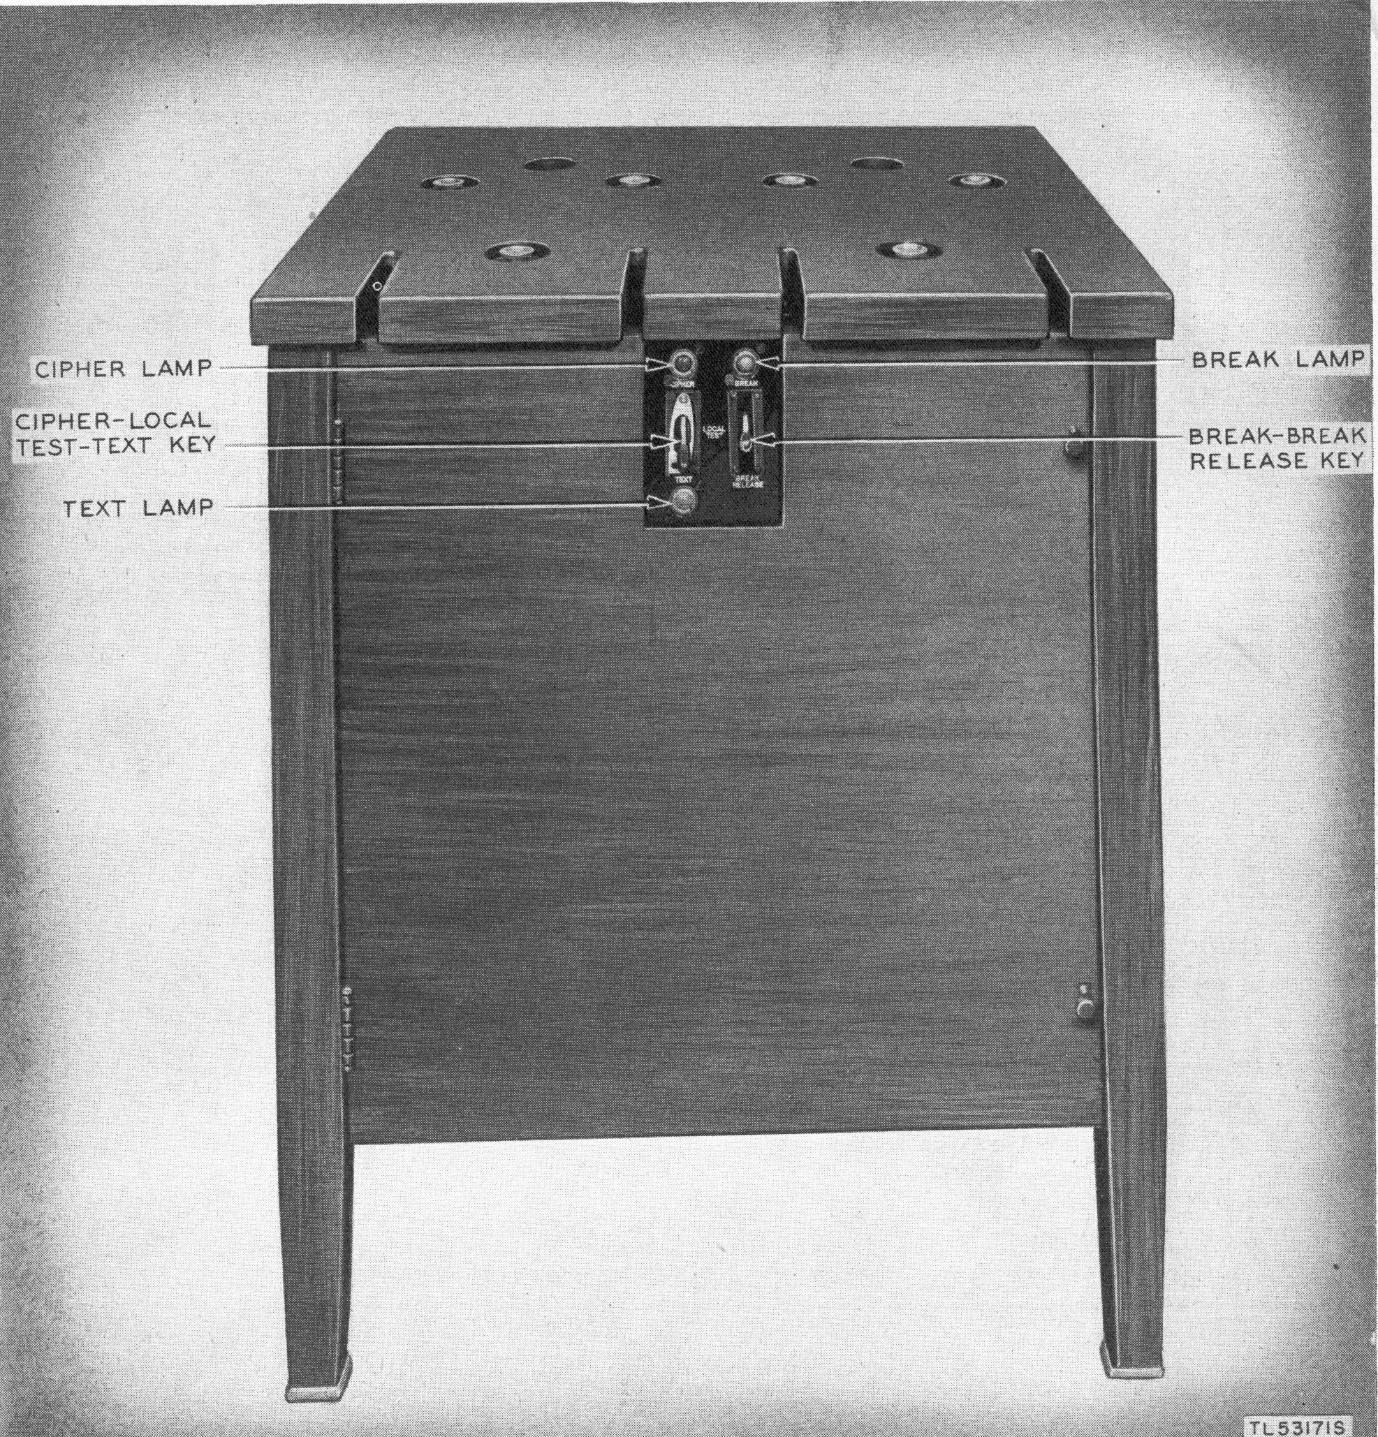
\includegraphics[width=0.8\textwidth]{images/ch1_Intro/MIxer.jpg}
    \caption{\textbf{AN/FGQ-1 Mixer}. Two-way teletypewriter repeater and mixer equipment enclosed in a wooden Table-type cabinet.} \label{fig:Mixer}
\end{figure}

This machine is a kind of a box, and next to the box was seat a wireless
operator with a typewriter, and the tape that came out from the typewriter was
with holes that spooled into the box together with another piece of tape, which
was the key. Inside the box were little lights that shine through the holes, and
little punches which would punch holes in the third piece of tape – the XOR of
the plain text and the key, and this is the output of one operation of the
machine. Afterward, the wireless operator feeds the ciphertext into the digital
radio to transmit.

Is the machine classified? If the system is designed right - you can reveal the
adversary whatever you want except for the secret key, and the system will
remain secure.

So, these machines were used during the war, until they break down, and at the
time that happened, they have been sent to the Bell Labs (which produced the
machines). The engineers who tried to repair one of the machines sat in a room,
and on the other side of the room, there was an \textbf{Oscilloscope}. 

An Oscilloscope is like babies monitor - just for signals. You connect the
Oscilloscope to an electric circuit, and there is a line that rising every time
there is a difference in voltage. \Cref{fig:Oscillo} demonstrates such a setup.
This Oscilloscope was not connected to the mixer, it was just laid at the other
side of the room, connected to some other test equipment. The engineers
discovered that every time this mixer enter the digit into the tape, they would
get a pulse at the Oscilloscope. When you send a current into an electric
monitor, the current is moving through the conductor and electromagnetic current
is being generated. The Oscilloscope has little wires, and the electromagnetic
waves traveling through these wires. As a result, we have a transmit antenna and
a receive antenna, so the Oscilloscope measures the holes (the ciphertext) in
the tape. Another possible explanation - when the punches punch a hole in the
tape, it consumes so much current that the voltage in the room drops a little,
and then the lines in the Oscilloscope – without being connected to anything -
just jumps.

\begin{figure}
    \centering
    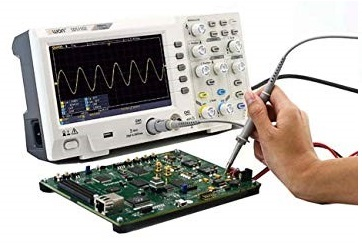
\includegraphics[width=0.8\textwidth]{images/ch1_Intro/oscilloscope.jpg}
    \caption{\textbf{Oscilloscope}. An electronic test instrument which graphically displays varying signal voltages as a function of time.}
    \label{fig:Oscillo}
\end{figure}

The engineers discovered~\cite{NSAsecret} that the top-secret information inside
this machine was being transmitted over the air. The process the engineers were
supposed to do is called responsible disclosure, meaning to report a bug. Like
good engineers, they told the Secret Service people about this bug, but they
didn't take their diagnosis seriously. So what did they do? The Bell labs were
located next to the U.S Secret Service office, so they set up an antenna and
they listened for an hour for radio transmissions that the Secret Service got in
their office, and they gave the Secret Service their ``top-secrets" analyzed
messages.

Obviously, the U.S Secret Service realized that the reported attack was not
esoteric, and they asked for a solution from the engineers. The solution of Bell
labs was to modify the mixers – to surround them in a wire cage which will
swallow the radiation that coming out from the machine, to put a shield on the
machine (to make sure the power consumption is not affecting the outside), and
to make sure that people are not getting close to the machine more than 30
meters. The Secret Service people decided to accept just the distance solution
and not the filtering/shielding/isolation solutions, because of the high
expenses and time that will cost to modify all the machine during wartime.

In 1954, the Russians published a tender to build military phones. They were
very strict about protecting the phones by shielding them and making sure they
don't generate too much radiation. In parallel, they were publishing tenders for
things like engines, turbines, etc. and they didn't were so strict for that
tenders. This is an evidence to that in those years, the Russians know about the
``bug". In conclusion, a one-time pad is the most secure cipher known, but from
the story above, we can see it was broken. So, what was broken? \textbf{The
implementation}.

Here are a couple of other machines which will break using attacks on their
implementation:

\begin{itemize}
    \item \textbf{Xbox 360}: Xbox is a PC that plays nothing but games, it is
    very cheap and you pay for the games. Attackers, obviously, want to crack
    the Xbox – to play games for free, to watch movies on the device or to run
    Linux. In Xbox there are some integrity checks, and one of the checks was
    done by a command called ``memory compare"~\cite{memcmp}, so you would
    calculate the integrity check over whatever software it supposes to run and
    you would have it stored in the secure memory, and then you would try to
    compare using these 2 values. This command leaks the length of the number of
    correct bytes before the first incorrect byte, so if you compare 2 blocks
    and the first bit is different – the response will be fast, and if the
    blocks identical until the very last bit – it would take a longer. This is
    one of the things that was enough to break the machine. 
    \item \textbf{Oyster Card}: it's a computer without power supply and Inside
    this computer that are stored values. Attackers could attack this card to
    take the train for free. There are a lot of ways to attack the implantation
    of that card~\cite{garcia2008dismantling, courtois2008algebraic}.
    \item \textbf{Car Keys}~\cite{relayAttack}
    \item \textbf{FPGA}~\cite{fpga}: a piece of hardware which is a very
    versatile, meaning we can find it many kinds of hardware – routers, audio
    equipment, spaceships, etc. the FPGA has a firmware installed inside, and if
    you want to copy some designs you need to find the firmware. The firmware is
    encrypted, but a bunch of Germans researches
    discovered~\cite{moradi2011vulnerability} that if you measure the power
    consumption of the FPGA while it is encrypting the firmware – you can find
    out what is the key.
\end{itemize}

When we implement an algorithm without being careful, we can be exposed to
implementation attacks. To protects against these attacks, we must protect the
implementation and do countermeasures, but as we saw at World War II, those
countermeasures have a price, thus making the system more expensive, and they
make the system heavier.

\section{System Implementation} \label{sec:SystemImpl}

The simplest form of a computational system is a device which gets input, makes
a computation and finally produces an output as can be seen in
\Cref{fig:SecDev1}. We assume that our system contains a secret, which cannot be
revealed to anyone before, during and after the computation process. 

\begin{figure}[!ht]
    \centering
    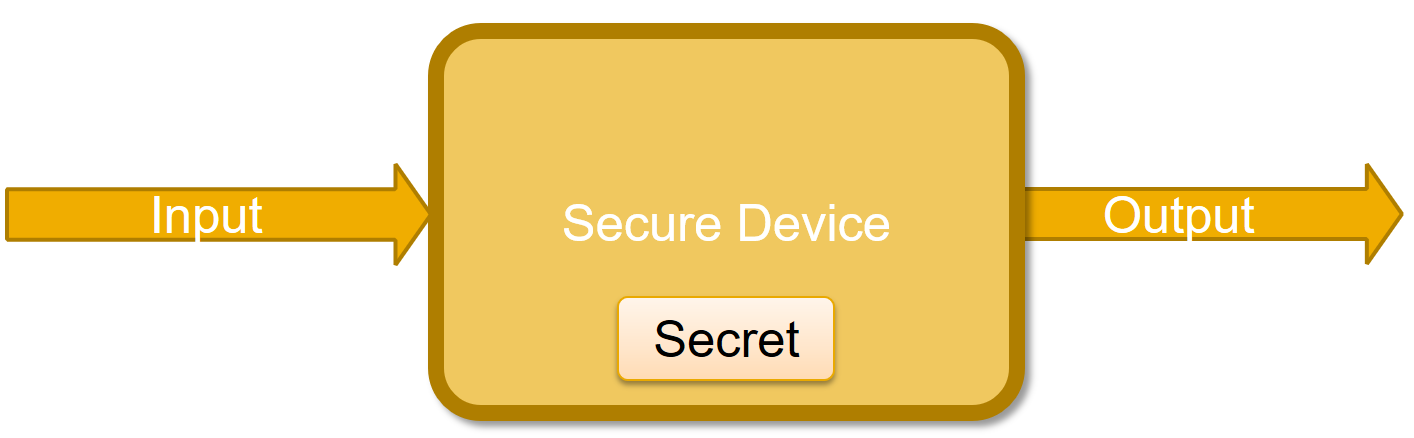
\includegraphics[width=0.8\textwidth]{images/ch1_Intro/Secure_device1.png}
    \caption{\textbf{Simplest Model}. The device make a computation using the secret and the input, and outputs the result.} \label{fig:SecDev1}
\end{figure}

But, if that all what the ``system" has, it is not a system, it is just an
Algorithm. What turns an algorithm to be a system? It's implementation.

Think about ATM – very simple device without cryptography. The input is our
credit card and a 4-digits PIN code, the output is money. If we don't know the
PIN code we can go over the all possible combinations of 4-digits code (brute
force), and finally find the correct PIN. Unfortunately, we have a limit of 3
trials until the card is being shredded. What an attacker can do?

As an output, and besides the money, we have also some additional outputs which
have been produced by the implementation of the physical system. Those
additional outputs are called ``Side Channels" and they are outputs which the
system designer did not intend to produce. Those outputs are demonstrated in
\Cref{fig:SecDev2}

\begin{figure}[!ht]
    \centering
    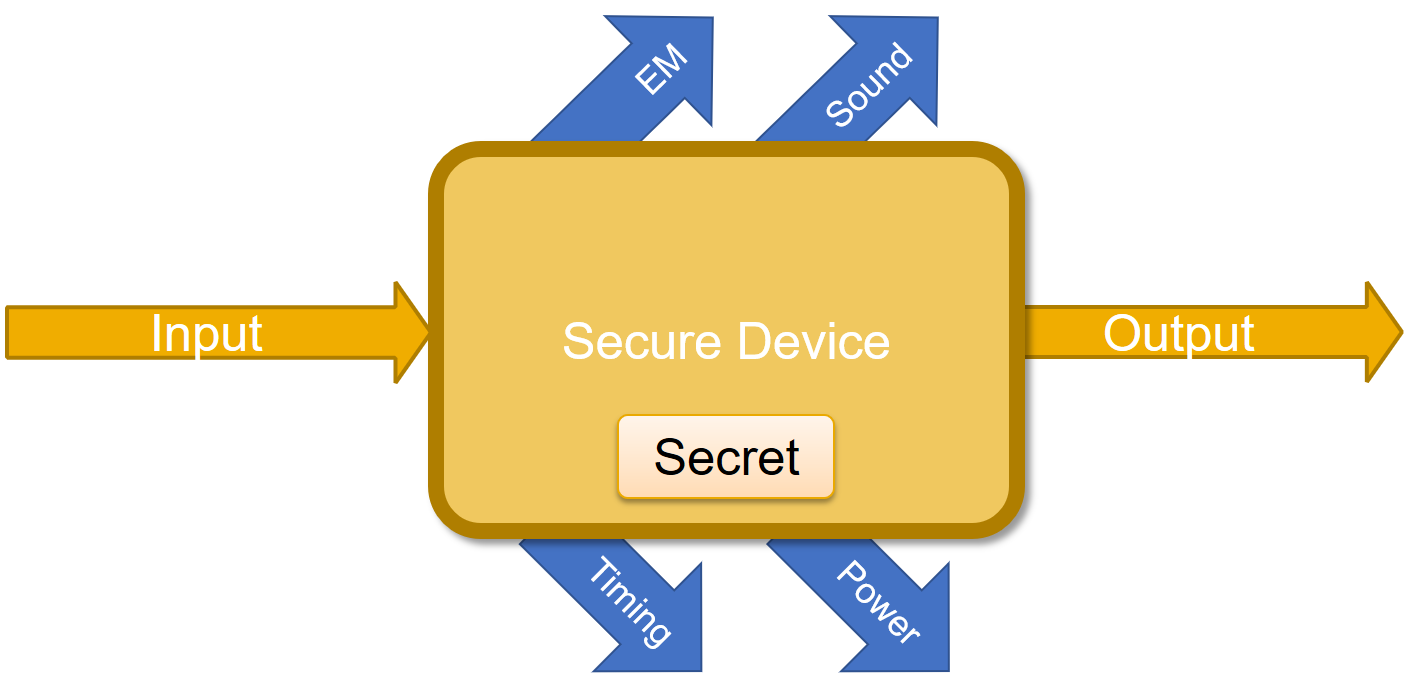
\includegraphics[width=0.8\textwidth]{images/ch1_Intro/Secure_device2.png}
    \caption{\textbf{Side Channels of the System}. Caused by the implementation of the system}
    \label{fig:SecDev2}
\end{figure}

For example, we can measure the time it takes to fulfill the operation,
electromagnetic radiation, the sound of the device while the operation is being
fulfilled, power measurements, etc. These are \textbf{Passive Attacks} – meaning
we are letting the device to do his stuff while we just listening.

There are also \textbf{Active Attacks} – called also fault attacks -  try to
break the device in a way that it will be ``just a little broken" – ruin the
device's activity in some way. It can be by turn it off in the middle of
calculation, change his clock, etc. As a result, we will maybe not get the
actual secret, but we will get some kind of errors that can teach us a lot about
the secret. 

\begin{figure}[!ht]
    \centering
    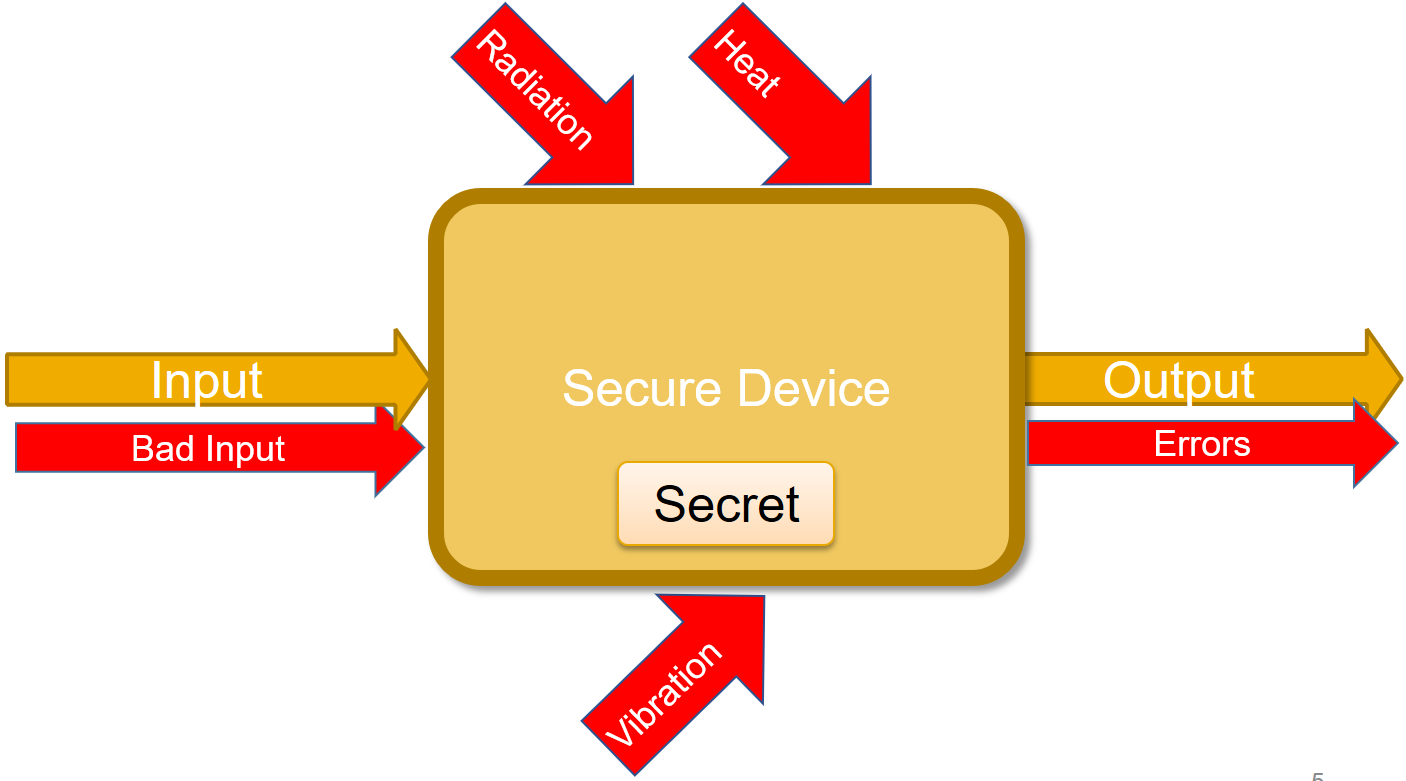
\includegraphics[width=0.8\textwidth]{images/ch1_Intro/Secure_device3.png}
    \caption{\textbf{Fault Attacks}. Manipulating the device through side channels}
    \label{fig:SecDev3}
\end{figure}

\section{Security of a System} \label{sec:SystemSecurity}

When we can say that a system is secured? Usually, we define a system as a
``secured system" if the system maintains three aspects of information security,
known as the CIA~\cite{cia} triad:

\begin{itemize}
    \item \textbf{Confidentiality} - when you are interacting with a system, you
    only get what you wanted to get. For instance, when I check my test grade,
    I'll get my grade and not my friend's grade. A possible attack could be data
    leakage.
    \item \textbf{Integrity} - all the data in the system is correct. A possible
    attack could be that one side of the communication will accept a message
    they are not supposed to accept.
    \item \textbf{Availability} - the system must work (in a reasonable time). A
    possible attack could be a Denial of Service (DOS).
\end{itemize}

In \Cref{fig:CIA} the relation between those aspects is demonstrated as the
Triangle of Information Security.

We don't have to use cryptography to secure our system. For example, if someone
goes to some event without invitation, there is a security to prevent him from
getting in.

An \textbf{Algorithm} is a process or set of rules to be followed in
calculations or other problem-solving operations. An example of an algorithm is
GCD/Extended GCD. An algorithm is secure when it is implementing the CIA triad
mentioned above. A \textbf{Protocol} is when you need to get something done, for
example, AES -  the input is a 128-bit key and a 16-bytes plaintext (in case of
more than 16-bytes we should use padding), and the output is a ciphertext.

\begin{figure}
    \centering
    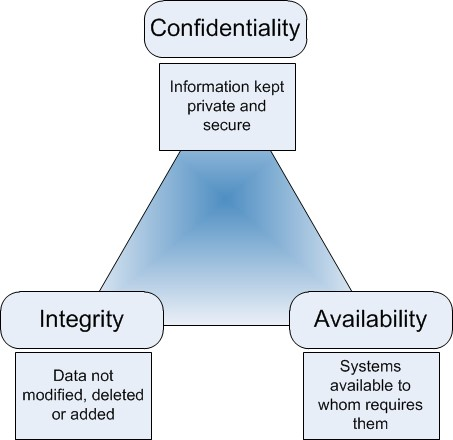
\includegraphics[width=0.5\textwidth]{images/ch1_Intro/cia.jpg}
    \caption{\textbf{CIA Triangle}. The classic model for information security. Defines three objectives of security: maintaining confidentiality, integrity, and availability. Each objective addresses a different aspect of providing protection for information.}
    \label{fig:CIA}
\end{figure}

The millionaire problem~\cite{lin2005efficient} is a classic problem by Yao and
it is an example of a protocol – this problem asks whether two millionaires can
learn who is richer, without revealing to one another how much money they each
have. One possible solution, they could invite a poor man, tell him in secret
how much money each has, and the poor man will announce who is richer.  

Cryptographically Secure Algorithms and Protocols:
\begin{itemize}
    \item \textbf{Encryption and Decryption} - Public key-RSA, Symmetric key-AES
    \item \textbf{Signing and verification} - must be an asymmetric key. There
    are 2 parties – signing party and verifying party (who gets the public key).
    The difference between signing and decryption is when one side sends a
    signed message it comes with a signature, and when one side decrypts a
    message he is sending only the ciphertext.
    \item \textbf{Key Exchange} - Diffie Hellman algorithm.
    \item \textbf{Hashing and HMACs} - a hash is a function that gets a long
    input (the length doesn't matter) and outputs a fixed size output. A hash
    function is secure when it's hard to find collisions, e.g. 2 messages with
    the same hash. HMAC is a hash with a key – when you change the key, the hash
    is changed.
    \item \textbf{Multiparty Computation}
    \item \textbf{Cryptocurrency}
\end{itemize}

Secure Architectures without cryptography:
\begin{itemize}
    \item \textbf{Secure Policies} - like access control to a military base, for
    instance.
    \item \textbf{User Separation and Sandboxing} - a program is divided into
    parts which are limited to the specific privileges they require to perform a
    specific task.
    \item \textbf{Virtual Memory} - application has a view of the memory, and we
    can take to pointer and point to some parts of the memory. We will get our
    old memory (which I'm allowed) or the app will crash due to access to
    invalid memory space. In theory, we can't get another user memory.
\end{itemize}

\section{Constructing and Using a Threat Model} \label{sec:BreakImpl}

What is the main advantage we have as attackers which allowed us to break
implementations that are secure in theory? The main advantage is that we have
more inputs and outputs – side channels, leakage – and together it means that we
can break a completely secure algorithm. But when is an algorithm's
implementation secure? CIA triad still holds, but the thing that missing here is
the \textbf{story}, i.e. what are we allowing the adversary to do with my system
– the more power we give the adversary the attack becomes less impressive. 

Let's have a look at a little system where the assumptions were broken:

\begin{figure}[!ht]
    \centering
    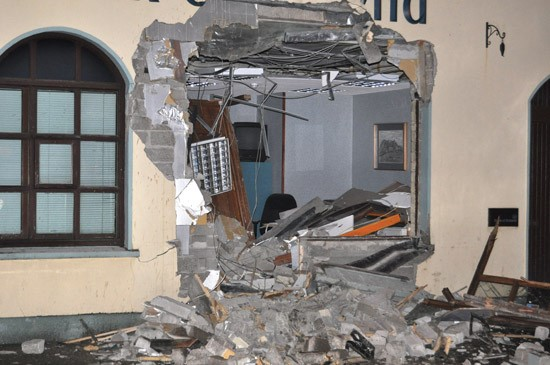
\includegraphics[width=0.8\textwidth]{images/ch1_Intro/Bank.jpg}
    \caption{\textbf{ATM theft.} The thieves simply ripped the machine out of the wall.}
    \label{fig:Bank}
\end{figure}

\Cref{fig:Bank} presents a wall of a bank in Ireland, which an ATM was
constructed on it. As we know, the ATMs are very secure systems – they have
encryption, they check our ID very carefully and if we make any mistake they
shred the card. What happened is that the ATM was stolen from the wall of a bank
by thieves which took a digger and smashed through the wall, put the ATM on
their track, and laid the digger across the road to prevent the police from
chasing them. We can learn from this story, that the ATM was secure, but their
threat model was wrong.

The most important thing about the threat model is the story. If the story is a
thief which comes to the bank in the middle of the night with a digger it's one
story, and if a thief comes in the middle of the day by foot, it's a different
story. Once we have the story, we can detail what are the properties of the
story. We divide them as follows:

\begin{itemize}
    \item \textbf{Victim Assets} - what the victim have that I want to steel? 
        \begin{itemize}
            \item \textbf{Cryptographic secretes (keys)} -  the keys are short,
            and when one steals the key – the attack has succeeded. There are
            two kinds of keys, long term, and short term.
                \begin{itemize}
                    \item \textbf{Long term key } - the private key that
                    identifies a server. If one steals this key, he will be able
                    to sign malware as a software update.
                    \item \textbf{Short term key} - a key that generated during
                    a session start from the long-term key. If one steals this
                    key, he can decode all the messages in the current session
                    and modify/inject them.
                \end{itemize}
                Notice that if one steals the long-term key it doesn't mean he
                can steal the short-term key.
            \item \textbf{State secrets} - for example, ASLR or configuration of
            a system. If one can find out the addresses of functions in the
            memory of a victim, he can write exploits. 
            \item \textbf{Human secrets} - things which the users do not want to
            expose like passwords, medical condition, etc.
        \end{itemize}
    \item \textbf{Attacker Capabilities} - what can the attacker do?
        \begin{itemize}
            \item \textbf{Off-path} - the attacker sitting somewhere in the
            world – can't observe or communicate with you, but he can attack you
            somehow. 
            \item \textbf{Passive Man in the Middle} - attacker who can see the
            victim communication with the server, for example, but he cannot
            communicate with the victim directly.
            \item \textbf{Active Man in the Middle} - an attacker who can
            interact with the server and can do replay attacks.
            \item \textbf{Physical Access} - an attacker who has physical access
            to the victim. For example, removing or unplugging or melting stuff
            in the system.
        \end{itemize}
        An important thing we need to consider when we are talking about
        attacker capabilities is the other defenses we must protect our system –
        guard or camera, for example. Another thing is the scale of the attack –
        how many systems can we attack at once. If the attack is physical,
        probably just one system. If the attacker attacks from an android app,
        maybe he can attack all the phones in the world.
    \item \textbf{Attacker Objectives} - who are the attackers? What do they
    want?
        \begin{itemize}
            \item \textbf{Stealing stuff} - the attacker might want to steal
            your secrets.
            \item \textbf{Duplicating stuff} - for example, the attacker can buy
            one smart TV card, and generate a thousand duplicates from this card
            to sell them. 
            \item \textbf{Forging stuff} - the attacker creates something new,
            driver licenses for instance.
            \item \textbf{Corrupting stuff} - the attacker breaks something and
            decommissioned the system.
        \end{itemize}
\end{itemize}

Of course, the more limits we put on the attacker, the attack gets more and more
impressive.

\section{Related Work} \label{sec:RelatedWork}
The whole topic of Attacks on implimitation has been widly reaserched,
and side channels attacks have been found on many varius types of implantation.
Here are a few interesting such types of side channels attacks
 and examples for actoual attacks on those topics:
\begin{itemize}
    \item \textbf{Audio-based attacks} - for example, ultrasonic beacons and acoustic cryptanalysis. 
    a type of side-channel attack that exploits sounds emitted by computers or other devices.
    Most of the modern acoustic audio-based attacks focus on the sounds produced by computer keyboards and internal computer components,
    but historically it has also been applied to impact printers and electromechanical deciphering machines.
    here are a few examples of real-life acoustic attacks: 
    \begin{itemize}
        \item \textbf{1} In 2004, Dmitri Asonov and Rakesh Agrawal of the IBM Almaden Research Center announced that computer keyboards and keypads used on telephones and automated teller machines (ATMs) are vulnerable to attacks based on the sounds produced by different keys.
         Their attack employed a neural network to recognize the key being pressed.
         By analyzing recorded sounds, they were able to recover the text of data being entered.
         These techniques allow an attacker using covert listening devices to obtain passwords, passphrases, personal identification numbers (PINs), and other information entered via keyboards.
         In 2005, a group of UC Berkeley researchers performed a number of practical experiments demonstrating the validity of this kind of threat.
        \item \textbf{2} A new technique discovered by a research team at \textbf{Israel's Ben-Gurion University Cybersecurity Research Center} 
        allows data to be extracted using a computer's speakers and headphones. 
        Forbes published a report stating that researchers found a way to see information being displayed, by using a microphone, with 96.5 percent accuracy.
    \end{itemize}
    \item \textbf{Differential fault analysis} those attacks take multiple traces of two sets of data, then computes the difference of the average of these traces.
    If the difference is close to zero, then the two sets are not correlated, and if the p-value (typically ≥ 0.05) is higher, correlation can be assumed to be possible.
    An example of an attack that was achieved by this is cracking the difficult-to-solve 128-bit AES. 
    Using differential fault analysis it was shown that the key can be broken into 16 bytes, where each byte can be solved individually.
    Testing each byte requires only 28, or 256 attempts, which means it would only take 16 x 256 or 4,096 attempts to be able to decipher the entire encryption key. 
    \item \textbf{Data remanence} Data remanence is the residual representation of digital data that remains even after attempts have been made to remove or erase the data.
    This residue may result from data being left intact by a nominal file deletion operation, by reformatting of storage media that does not remove data previously written to the media,
    or through physical properties of the storage media that allow previously written data to be recovered.
    Data remanence may make inadvertent disclosure of sensitive information possible should the storage media be released into an uncontrolled environment (e.g., thrown in the trash or lost)
    an example of an attack that is using data romance is cold boots wich steals sensitive cryptographic materials like cryptographic keys by Keeping DRAMs at lower room temperature,
    say -50 degrees C, and making it hard for the Dram to preserve his data properly.
    more details on this attack can be found here \href{https://resources.infosecinstitute.com/cold-boot-attack/#gref}{cold-boot-attack}.
    \item \textbf{Optical attacks} these attacks range from the relatively simple (eavesdropping on a monitor via reflections) through to complex (communicating with an infected device via LED blinks). 
    An article of optical attack utilizing the photonic side-channel against a public-key of common implementations of RSA \href{https://www.eng.tau.ac.il/~yash/ieee-host-2017.pdf}{optical side-channel against a public-key of RSA}.
\end{itemize}

In addition to those attacks, there are even more side channels attacks research and new weaknesses are discovered every time.
More of such attacks like Specter, RowHummer, and many more will be described widely in this course.
  
    





\chapter{Temporal Side Channels I} 

\section{History}
In 1995, at the age of 22, Paul Kocher released a paper called Timing Attacks on
Implementations of Diffie-Helman, RSA, DSS and other
systems~\cite{kocher1996timing}.

Before it was published, he wrote about it in a mailing list of
Cypherpunks\footnote{A cypherpunk is any activist advocating widespread use of
strong cryptography and privacy-enhancing technologies as a route to social and
political change. Originally communicating through the Cypherpunks electronic
mailing list, informal groups aimed to achieve privacy and security through
proactive use of cryptography} which included all sorts of people like
mathematicians, photographers, artists anarchists and more. The attack was first
demonstrated in 1997 at a cryptography conference. And later, in 1998 an
academic paper was published describing how to perform the attack.
In 2003 and 2007 this kind of attack was used to break SSL.



\section{The Threat Model}
The objective of the attacker is to discover the password. The attacker goes about this by sending
unlimited queries and measures their time.
Unlimited queries are not always possible. Some devices are disabled after three to five tries.
The same applies to time measurements.
However the assumption is that these are possible according to Kerckhoffs's principle(law), 
that states that everything except the key is public knowledge. 

Figure \ref{c1_fig_threat_model} describes the Threat Model on an implementation
of a secure system. It is important to mention that we're talking about
attacking an implementation, and not the algorithm itself as we consider the
algorithm or protocol being examined as completely secure.

\begin{figure}[H]
    \centering
    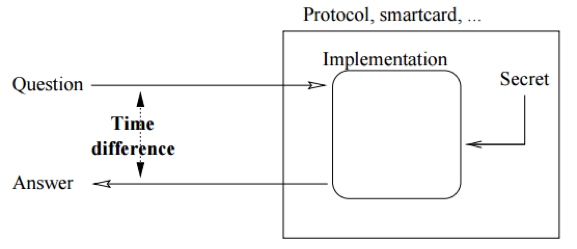
\includegraphics{images/chapter_1/threat_model.png}
    \caption{The Threat Model. Image from JF Dhem1998. The attacker can send a
     message to the implementation and get an answer from it. Also - the
     attacker is able to measure the time it takes for the implementation to
     compute the output}
    \label{c1_fig_threat_model}
\end{figure}

\subsection{When is a timing attack even possible?}
\begin{enumerate}
    \item Physical access to the device. (for example: Smart card, Crypto
    wallet, Electronic voting machines)
    \item Sharing a virtual machine with the service (for example: Swiping a
    credit card)
    \item Remote access to a device (access to a device over the network, which
    may be very noisy and may be rather difficult to implement)
\end{enumerate}



\section{Timing attack}
    A timing attack is based on the time it takes to complete an algorithm.


\begin{figure}[H]
    \centering
    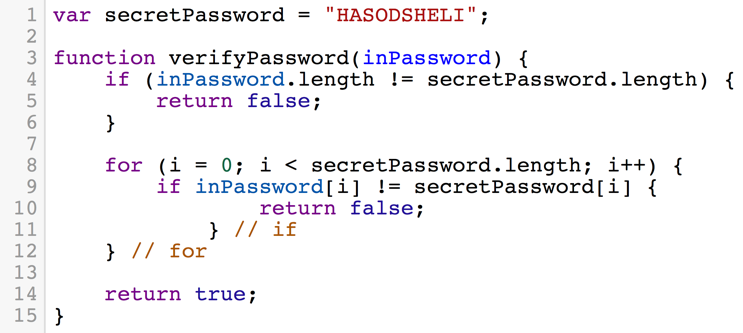
\includegraphics{images/chapter_1/password_check_algo_1.png}
    \caption{A simple and efficient password checking algorithm. In line 4
    there's a check if there length of the password is the same as the length of
    the input. In line 8 there's an iteration over all of the characters in the password
    }
    \label{c1_fig_pass_check_1}
\end{figure}

Consider the algorithm for password checking as described in figure
\ref{c1_fig_pass_check_1}

In a scenario where a timing attack is not possible, breaking the password
 requires the attacker to bruteforce the password, checking every
 possible string for one successful attempt.

Let's assume the password is the length of 16 characters, and if the password only contains english
upper-case characters we have 26 possible values for each of the 16 characters
in the password. The first character has 26 possiblites, the second has 26
possiblites and so on. So bruteforcing a password like this requries ${26}^{16}$
different attempts, which cannot be completed by any computer in a decent amount
of time. In general, for a password of length $n$ and character range of size
$k$, breaking the password will take $O({k}^{n})$ attempts.

Now let's consider the scenrio where \textbf{a timing attack is possible}. To
perform a timing attack, the attacker takes advantage of the fact that when the
program checks for strings equality, the comparison will finish as soon as it
finds one character that doesn't match. Consider the following example where the
attacker tries the 3 following attempts and measures the time it takes for the
machine to respond. The attacker tries "AAAA" and measures 0.2ms, then tries
"BAAA" and measures 0.5ms lastly tries "CAAA" and measures 0.2ms again. The
attack can be pretty sure that the first character is "B". Now, checking the
whole password does not require iterating of all possible combinations of
strings of size $n$. All it takes is to iterate over all possible values of each
character, say $k$, and repeat that $n$ times. This results in a total runtime
of $k+k+k+\dots = nk = O(n)$

We can now break the password in a reasonable amount of time, even without
knowing the length of the password we're trying to crack.

\section{Timing Attack Defenses}
After discussing the potential of such attack, we now consider the possible
mitigations we can implement on our system to prevent such attacks.

\subsection{Mitigation}
We can consider adding a random wait time after checking each one of the
characters. The problem of course is that the whole process of checking for a valid
password becomes slower. And of course, if the attacker can perform a lot of
measurements on our system, since the noise is random, the attacker would be
able to ignore it.


\subsection{Prevention}
The second type of countermeasure is prevention, making sure that our system is
completely resistant to timing attacks.

\subsubsection{Prevention Method 1: Padding}
\begin{figure}[H]
    \centering
    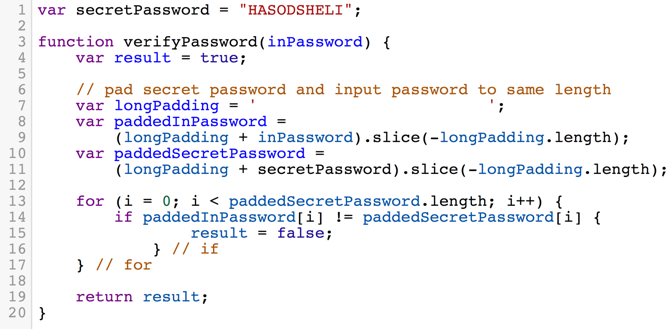
\includegraphics{images/chapter_1/password_check_algo_2.png}
    \caption
    {Prevention method 1, padding the user guess and the secret password to the
    same length and check all characters even if there's a mismatch in the first
    character.}
    \label{c1_fig_pass_check_2}
\end{figure}

The first method we examine is to pad the secret password and the user's guess
to the same length. Also - the function dosen't exit as soon as we see a character
mismatch. The code is described in figure 
 \ref{c1_fig_pass_check_2}

The problem with this implementation is that every time there's a character
mismatch we execute additional code, which is loading the variable
\lstinline{result} and writing the value \lstinline{false} to it. This may seem
insignificant in the beginning but actually, this makes our code \textbf{much
more vulnerable than it was before}. As now the time it takes for the entire
function to complete is linearly dependant on the amount of characters
mismatches we have, this allows an attacker to perform the same attack from
before with no significant changes to his original timing attack.

One might think of a fix which is adding another branch to the \lstinline{if}
statement that will do some garbage operation like \lstinline{foo = false} just
so that the attacker might not be able to distinguish between a match
and a mismatch. The problem with this fix might be that the access time to one
variable may be different than the access time to another variable, and the
attacker will be able to tell the difference between them.


\subsection{Prevention Method 2: Hashing}
\begin{figure}[H]
    
    % \centering
    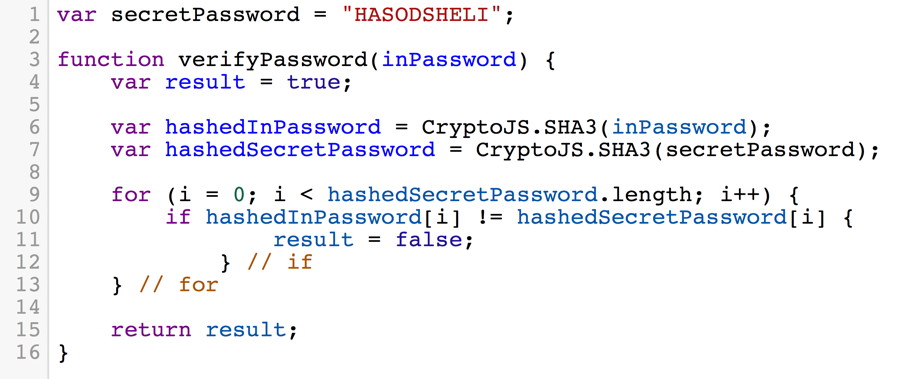
\includegraphics[scale=0.6]{images/chapter_1/password_check_algo_3.png}
    \caption{Secure password checking using a secure hash function}
    \label{c1_fig_pass_check_3}
\end{figure}

The right way to store passwords is with hashing (storing the hash of the
password rather than the password in plain text). A hash is a cryptographic
function which has the property called "The Avalanche Property" which means if
even 1 bit is fliped in the input, at least half of the bits of the output are
flipped as a result. This means that even if my guess is really close to the
password (1 bit away from the real password) I cannot really know which bits are
correct and which are not due to the Avalanche property.

Using hashes to perform a secure password check is described in the algorithm in
figure \ref{c1_fig_pass_check_3} A guess is being hashed before it is compared
against the hash of the true password. An attacker might use the same methods
as described previously to try to leak the hash of the true password, but that would be very
difficult as the attacker does not input the hash, the attacker only controls a
string that is later being hashed by the algorithm. So trying the previous methods
to leak the password would not work assuming the hash function is propely
implemented. 

A possible leak occuring from this method is the length of the true
password. In line 7 of the algorithm in figure \ref{c1_fig_pass_check_3} the
hash of the true password is computed. Line 7 makes the total run time of the
program dependent upon the length of the true password. While this might be risky,
this is easy to fix - we can just precompute the hash of the true password and
use it whenever the algorithm runs. This is done for example in Linux where the
hashes of user's passwords are stored in a file in \lstinline{/etc/shadow}.


\section{The Algebra Behind RSA}
The next thing we're going to perform a timing attack on is the RSA crypto
system. But before we delve into how we break RSA (next chapter) we're going to
discuss the algebraic foundation of RSA~\cite{kaliski2006mathematics}.

The RSA cryptosystem lives in something called a multiplicative group. The group
that is $Z^{*}_n$.

We're taking 2 random prime numbers; $p$, $q$ and assign $n=pq$. The group
$Z^{*}_n$ contains all the numbers from 1 to $n-1$ which do not divide $n$ (that
is, do not divide $p$ or $q$). For example: for $p=3$ and $q=5$, $n= 3*5 = 15$
so $Z^{*}_n = {\{1,2,4,7,8,11,13,14\}}$.

Like all groups, this group has the associative operation which in our case is
the modular multiplication, that is because we mentioned before that this group
is a multiplicative group. The group is also closed under that operation.

The group also has an identity element, 1. Which when multiplied by another
element from the group - does not change it.

The last property this group has is that every element $r$ in the group has an
inverse element $r^{-1} \in Z^{*}_n$.

Since the exponentiation is just repeated multiplication - we consider
exponentiation to also be a closed operation under that group. Each element has
an order, the order always divides $(p-1)(q-1)$ (Fermat's little theorem). When
the element is raised to the power of the order, the result of the exponentation
(under the modulu of course) is 1, the identity element in the group.

It also important to note that we cannot compute $(p-1)(q-1)$ from knowing $n$

\subsection{Elementary Operations of RSA}
To use the RSA crypto system to encrypt and decrypt messages you first have to
generate the infrastructure. That is deciding on $p$ and $q$ both large prime
numbers and computing $n = pq$ and $(p-1)(q-1)$ denoted as $\phi(n)$

\begin{itemize}
    \item \textbf{Choosing a public and private key pairs}
    Choose $e \in Z^{*}_{\phi(n)}$, $d \in Z^{*}_{\phi(n)}$ such that $ed = 1$
    mod $\phi(n)$. The public key is the pair $\langle{n,e}\rangle$  and the
    private key pair is  $\langle{n,d}\rangle$.
    \item \textbf{To encrypt a message}
    Choose $m \in Z^{*}_n$ as your message. The cipher is $m^{e}$ mod $n$ = $c$
    \item \textbf{To decrypt a message}
    Since $c = m^{e}$ mod $n$, perform $c^{d}$ = $m^{ed}$ = $m^{1}$ = $m$ mod
    $n$
\end{itemize}

Example: Consider $p = 3$, $q = 5$. So we can compute $n = 3*5 = 15$ and
$\phi(15) = 2 * 4 = 8$ Let's assume we choose $e = 3$ and $d=11$. We consider
the message 2.

To encrypt, we compute $2^{3} = 8$ mod 11, Which is the cipher. And to decrypt,
we're using the private key $11$ as follows: $8^{11}$ = 2 mod 15. And now we
have our message back, 2.

Since this is not a crypto course, we will not go into any more details
about the algebra behind RSA. However it is important for us to familiarize ourselves
with the basics of RSA in order to understand later how it was optimized and how
can we break it.

\subsection{See also}
\begin{enumerate}
    \item John Wiley and Sons Chichester , "Overview about Attacks on Smart
    Cards by Wolfgang Rankl, Munich", 3rd edition at John Wiley and Sons in
    September 2003.
    \item Thomas Popp, "An Introduction to Implementation Attacks and
    Countermeasures", Graz University of Technology, Institute for Applied
    Information Processing and Communications (IAIK) Graz, Austria.
\end{enumerate}

\chapter{Temporal Side Channels Part 2} \label{cha:Temporal Side Channels Part 2}

\section*{recap}\label{sec:recap}

In the previous chapter we discussed about RSA cryptosystem~\cite{wikiRSA}. In this chapter, we
presented the most expensive operation in the RSA algorithm which is when we need to take the
message (m) and raise it to the power of the key.
\[ C = m^e(modn) \] The simplest algorithm for raising a number to a power uses
modular multiplication which is an expensive operation.

\begin{figure}[!ht]
    \centering
    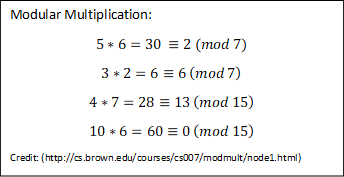
\includegraphics{images/modmul.png}
    \caption{Modular multiplication} \label{fig:modmul}
\end{figure}

Modular multiplication is pretty straightforward. It works just like modular
addition. You just multiply the two numbers and then calculate the standard
name. Examples for Modulo 7 and 15 can be found in \Cref{fig:modmul}. Why
modular multiplication is so expensive? Because we have to take the modulo many
times which is as expensive as division\footnote{Division is the most expensive integer
operation exists, and  therefore we don't want to do many divisions}. So, one way
to do this is by keep multiplying and doing the modular reduction only at
the end. The problem with that approach is that the runtime of multiplication grows exponentially
with the number of the multiplicands. 
Another way is to do a \( mod n \) with each multiplication, but the numbers keep growing 
and the runtime keep raising, so we can't do that either. 

\begin{figure}[!ht]
    \centering
    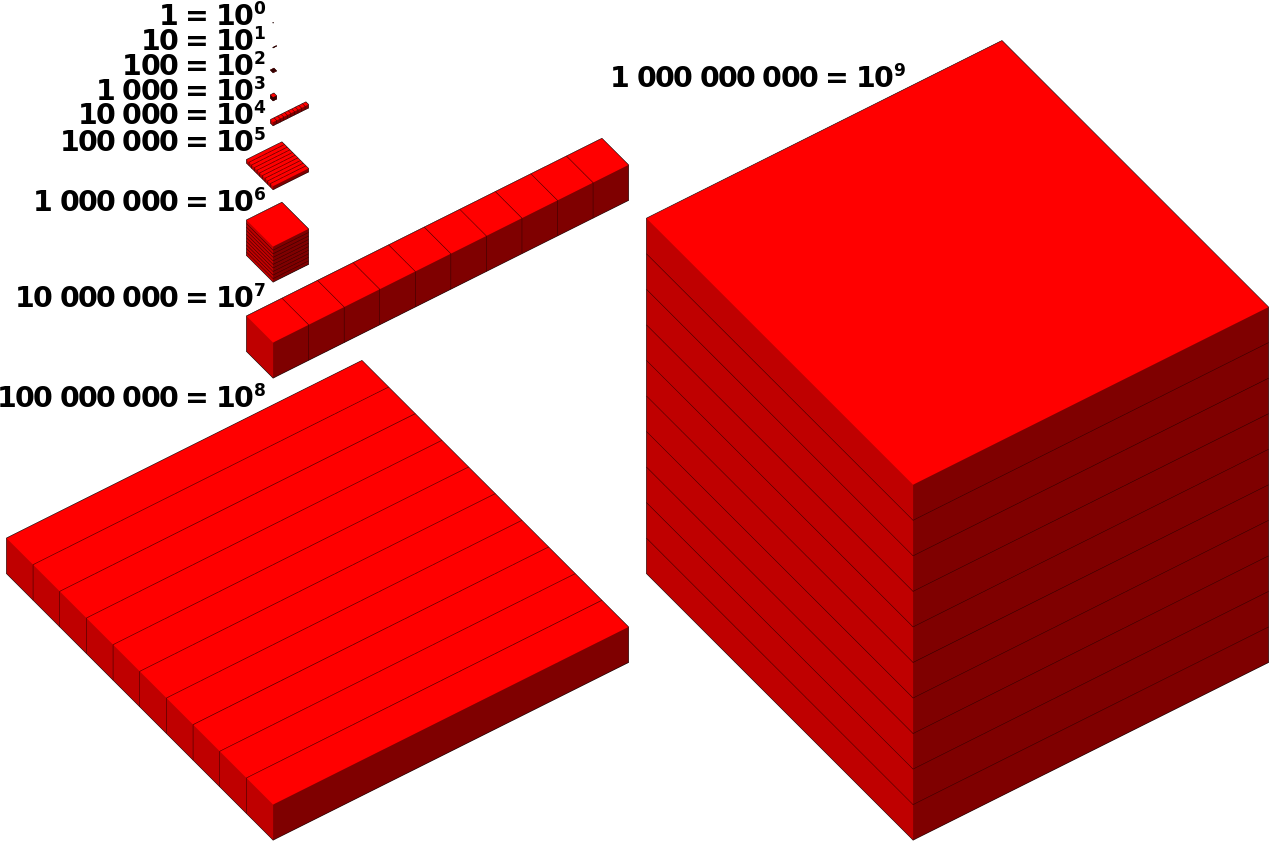
\includegraphics[scale=0.25]{images/vispow10.png}
    \caption{Visualization of powers of 10 from one to 1 billion.} \label{vispow10:fig}
\end{figure}

As we discussed in the last chapter, the slowest and most trivial way of
implementing modular multiplication \(g^e mod n\) is to take $g$ and multiply it by itself
$e$ times, and every once in a while do modulo $n$, 
(either every multiplication or just in the end). The problem with this is
that if $e$ is a number that consists of 1024 bits, then in the worst case 
 we might need to multiply $g$ in itself \( 2^{1024} \) which is a huge number.

\section{Efficiently Implementing Modular Exponentiations}\label{sec:Efficiently Implementing Modular Exponentiations}

There are two ways for efficiently implementing modular exponentiations:
\begin{enumerate} 
\item performing fewer modular multiplications (instead of  \( 2^{1000} \)  we would
    like to do 1000). 
\item Make each modular multiplication to be less expensive. 
\end{enumerate} 
The best case would be same as regular multiplication over integer.
These two ways will reduce the cost of modular multiplication and modular
exponentiations, and this is something we really want to do in order to make RSA work on
a device.

So, assumeing we are engineers, we want to implement modular exponentiations very
cheaply. The right thing to do is obviously use some crypto library, but
let's assume that's not possible, and we are inventing a new CPU. There is a very 
famous book online called the handbook of applied cryptography
(\Cref{fig:appliedCrypt})~\cite{katz1996handbook}. The book is like a recipe book,
and is filled with algorithms, proofs and equations you need
for cryptography. Chapter 14 deals with efficient algorithms for multiplicative
proofs. The book contains several ways to do modular exponentiation. 

\begin{figure}[!ht]
    \centering
    
\includegraphics{images/appliedCrypt.jpg}
    \caption{Cover of the handbook of applied cryptography} \label{fig:appliedCrypt}
\end{figure}

The following approach is called the left to right binary exponentiation, also
known as square multiply.
\begin{figure}[!ht]
    \centering
    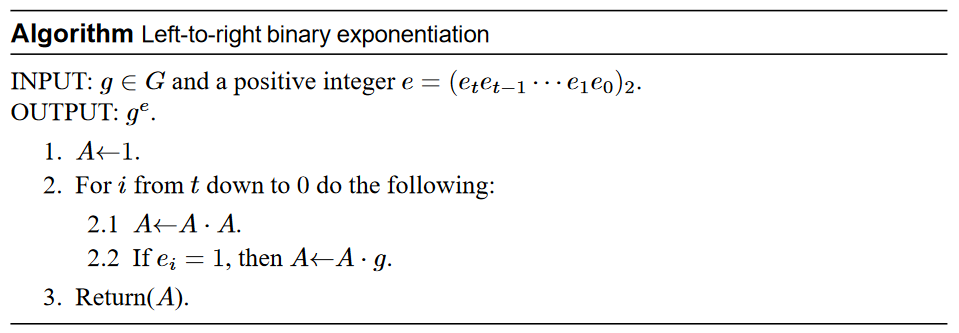
\includegraphics[scale=0.4]{images/ltrbe.png}
    \caption{The pseudo-code was taken from the handbook of applied cryptography, page 615.} \label{fig:ltrbe}
\end{figure}

The inputs are $g$ (we want to raise g to the power of $e$, \(g^e\)) and \(e\)
which is a bit string of $t$ ($t$ bits), (see \Cref{fig:ltrbe}). 
The most significant bit is always $1$, because there is no
logic behind raising something to the power of zero. In the end of this algorithm \(A\)
will be the result of $g$ raised to the power of $e$. 

In the beginning we set $A$ to be equal to $1$, and go over the bits from left
to right (from the most significant to the least). Each time we square $A$ ($A=A*A$),
but we only multiply by $g$ $(A=A*g)$ if the current bit is $1$ (the \( i^{th}\) bit).
Now, what happens when we do a squaring
operation downstairs? What happens to the exponent upstairs? Its multiplied by
$2$. So \({g^{e}}^2 = g^{2e} \)  and  \(g*g^{e} = g^{e+1} \). Now, we can think
of a binary string, you can write down the bits using shifting (multiplying by
$2$ is shifting) and adding $1$ is just putting one in the place.

So how many modular multiplications will be performed in order to raise g to the
power of $e$? The answer is \(O(t)\). In the best case - what is the lowest amount of 
multiplications that will be performed? the answer
is $t+1$ as the first bit is $1$ (most significant) so we do step 2.2 one time and
all the rest of the bits are zeros, and so we will only do step 2.1 in these cases. 
In the worst cast - what is the highest amount of multiplications that will be performed? 
Answer: $2t$, if all the bits equal to $1$ we will do $2$ multiplications for 
each bit (step 2.1 and step 2.2). In any case, this is equal to \(O(t)\),
so instead of \(2^t\) as in the old algorithm we perform at most $2t$
multiplications. 

Lets review an example. Lets calculate \(7^6=7^{(110)}\) in the group \(
\mathbb{Z}_{15}={1, 2, 4 ,7, 8, 11, 13, 14} \).

\begin{enumerate}
	\item  \(A = 1 = 7^(0) \)
	\item  \(A = A*A = 1 = 7^{(0<<1)} = 7^{(0)}\)
	\item  \(A = A*7 = 7 = 7^{(0+1)} = 7^{(1)}\)
	\item  \(A = A*A = 4 = 7^{(1<<1)} = 7^{(10)} \)
	\item  \(A = A*7 = 13 = 7^{(10+1)} = 7^{(11)} \)
	\item  \( A = A*A = 4 = 7^{(11<<1)} = 7^{(110)} \)
\end{enumerate}

Are there any ways doing this even faster? The answer is yes as we can see in the
handbook of applied cryptography. The general idea of
these algorithms is that we do some pre-computation. The idea of RSA algorithm is
that there is a public key $g$ that is a known number.
So if we know what $g$ is we can prepare all sort of lookup
tables. One method for doing that is called the window method,
where we take three bits at a time, and
instead of doing \(A*g\) we do \( A*g*g\) or \(A*g*g*g\) .. (8 values we can
use), and instead of \( A=A*A\) we do \(A=A*A*A\) and so on, this is the sliding
window. Another method is called the binary method, which is well described in
the handbook of applied cryptography (page 616 algorithm 14.83). We can assume 
that any reasonable crypto implementation is not doing the naive method.
It will use the left to right or the right to left binary exponentiation
which is basically the same idea as one of the window methods.

But what if we want the modular multiplication to be cheaper? A way to achive this 
is called the Chinese remainder theorem (CRT)~\cite{dingyi1996chinese}, named after 
Sun Tzu Suan that was a teacher from the \nth{5} century and
wrote a book that contained all sorts of riddles and questions.

The Chinese remainder theorem addresses the following type of problem. 
One is asked to find a number that leaves a remainder of 0 when divided by 5, 
remainder 6 when divided by 7, and remainder 10 when divided by 12. 
The simplest solution is 370. Note that this solution is not unique, 
since any multiple of 5 × 7 × 12 (= 420) can be added to it and the result
 will still solve the problem.
The theorem can be expressed in modern general terms using congruence notation.
 Let $n1, n2, …, nk$ be integers that are greater than one and pairwise 
 relatively prime (that is, the only common factor between any two of them is 1),
and let $a1, a2, …, ak$ be any integers. 
Then there exists an integer solution a such that 
$a ≡ ai (mod ni)$ for each $i = 1, 2, …, k$. 
Furthermore, for any other integer $b$ that satisfies all the congruences, 
$b ≡ a (mod N)$ where $N = n1n2⋯nk$. 
The theorem also gives a formula for finding a solution. 
Note that in the example above, 5, 7, and 12 ($n1$, $n2$, and $n3$ 
in congruence notation) are relatively prime. 
There is not necessarily any solution to such a system of 
equations when the moduli are not pairwise relatively prime.

Why does this help us? Allegedly, we have to do 2 operations instead of one. 
The way to do exponentiations in CRT is that we take our big number 
and do modulo $p$ and then modulo $q$ and then there is a CRT step. 
So what is the size of the operand used by these two modular exponentiations?
Assuming that $p$ and $q$ are of the same size? 
Let's say $p$ and $q$ are 1000 bits so the size of $n$ is 2000 bits
(we add the number of bits of each number in the multiplication).  So each
number in the multiplicative group is about 2000 bitw because it's mod $N$, so
multiplying two numbers is going to be multiplying two numbers which are 2000
bits. If we reduce it to modulo $p$ and modulo $q$ the numbers are going to be
half the size (1000 bits). So if we take a multiplication and now we will
multiply two numbers that are half the bit length what will be the speed
 improvement? 
 It's times 4. Instead of one big modular exponentiation we have one small
modular exponentiation which costs quarter of the time and another one which
cost quarter of the time followed by a CRT step which is a modular
multiplication of the two. 
How much we spent in total? Answer: a bit more than
half the time, twice speedup. 
Why can't we do that further? Divide $p$ and do it
again? Answer: because $p$ and $q$ are prime numbers and that's the whole point.

On top of that, there is a very nice trick, in order to make modular 
multiplications very cheap and this actually makes modular multiplications 
to be as cheap as regular multiplication.
Multiply two numbers is pretty easy but the
problem is reducing after multiplying. So what if there is a way of doing
modular multiplications without the reduction step? So in 1985 a genius
mathematician called peter Montgomery published a paper called ``modular
multiplication without a reduction step"
~\cite{warren2013hacker}\footnote{https://www.hackersdelight.org/MontgomeryMultiplication.pdf}.
The idea behind the paper is that we enter into a magical world 
called the Montgomery representation. When you step into the Montgomery world, 
modular multiplications do not require a reducing step and when you finish
you just step out of this world and you are back with your result. 
It's still cost you like a multiplication but it doesn't cost you the 
extra reduction step. So, what is the idea of the Montgomery reduction? 
We want to calculate \(g^emodn\) and to do that we need to pay a lot 
for modular reduction.
So, the first thing we do is enter the Montgomery representation and do the
Mont(\(g^e\)) and each one of this multiplication steps is going to be about as
difficult as regular multiplication (Figure Figure \ref{montg:fig}). After we
finished with that we exit the Montgomery representation and then we have our
result. Entering and leaving the Montgomery representation costs as much as
modular multiplication but in the middle it's as cheap as regular
representation.

\begin{figure}[!ht]
    \centering
    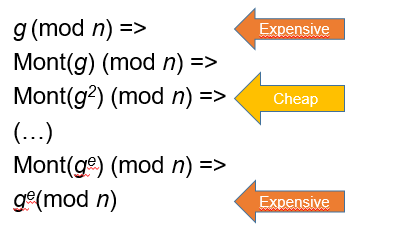
\includegraphics[scale=0.7]{images/montg.PNG}
    \caption{General sketch of Montgomery Exponentiation} \label{montg:fig}
\end{figure}

Now lets review how the Montgomery Exponentiation works inside
\begin{enumerate}
	\item  Choose a value R, \(R>n\), which is easy to use (usually a large
	power of 2)
	\item  \(Mont(a)=a*R(mod n) =^{def}  a(mod n)\)
	\item  \(Mont(ab)=a*b*R(mod n)=\underline{a}*\underline{b}*R^{-1} (mod n)\)
	\item  \( = (\underline{a}*\underline{b} +
	(\underline{a}*\underline{b}*n'(mod R)*n))/R(modn) \) \newline
	// if this is more than n, subtract n
	\item  \( A = A*A = 4 = 7^{(11<<1)} = 7^{(110)} \)
	\item  Result: Instead of modular reduction, we only (sometimes) subtract
\end{enumerate}

The first thing to do is to choose a very large value $R$ which is larger than
$n$ and should be easy to use ($a$ large power of 2) for instance 1 and 1000
bits of zero. What does it mean easy to use? To multiply and divide by a power
of 2 you just shift left and right. To calculate the modulo of a very large number
that is a power of 2 you do bitwise and with this large power of 2. if
$R=100000$ and $x = 10101010101110$ so to do a modular reduction we just take the
lower bits which are 01110 in this case. So we see it's very cheap operation with
$R$, but $R$ is not useful outside the situation. So to enter the Montgomery
representation we are going to multiply by $R$. This multiplication is modulo
$n$, and this is a bit expensive. But how do we know that $R$ is
inside the multiplicative group? How do we know that multiplying by $R$ doesn't
throw me outside of $mod n$? The answer is: how do we know that 2 is inside the
group? Because what is this group? This group is a multiple of two prime
numbers, and they are odd. Thus 2 doesn't divide either one of them so 2 is in
the group and \(2*2*2...2\) is in the group. We call the new number
\underline{a}. The idea is that the numbers in the Montgomery representation is
cheap so how is it cheap with \underline{a} If we multiply a and b in the
Montgomery's representation It will be: \(a*b*R mod n\). but if I want to do
that using \textbf{a} and \underline{b} we get:
\(\underline{a}*\underline{b}R^{-1}\)mod $n$ because of the extra R. So every
time we multiply two numbers we need to take out the extra R. Inverting $R$ is
simple using GCD and can be done before we start the computation. There are much
more derivations made to get to  \((\underline{a}*\underline{b} +
(\underline{a}*\underline{b}*n'(mod R)*n))/R(modn) \).
\underline{a}*\underline{b} is just a single multiplication.
\underline{a}*\underline{b}*n'(mod R) - Notice that \(modR\) is a cheap
operation because $R$ is 1 with lot of zeroes. ($n$ prime ($n'$) is just precomputed
number that doesn't really matter to us). 
Then we multiply it by $n$ (another multiplication) and then we divide it by $R$ 
which is also a simple operation. So,
we have 4 multiplications and we need a modular reduction which is the main
problem. Montgomery proofed that this sum is no more than \(2^n\). So how do you
do a reduction if the number is between 0 to \(2^n\)? You put an if statement.
If $x$ is less than $n$ you do nothing, if $x$ is larger than $n$ you subtract it
from the number n. So now, instead of division we do a couple of multiplications
over integers which is not that expensive and then we sometimes subtract. This
is a lot cheaper than the basic option and it is widely used. Notice that the if
statement in the algorithm, which is influencing the execution time and might 
enable a timing attack.

\section{Temporal Side Channel on RSA}\label{sec:Temporal Side Channel on RSA}

Let's review how to do a temporal side channel attack on RSA. Kocher described this
attack on his paper in 1995 among other things. If the RSA runs slower than
there are more subtractions and by timing the execution we can recover the key.
So how this can be done? How to recover the key by timing the execution? 
There was a fantastic paper ``A Practical Implementation of the Timing
Attack"~\cite{dhem1998practical} which the remainder of this section is based
on. So what is the game here? Assume you are an attacker who wants to commit a
timing attack on the secure implementation of RSA. If we have some device 
(e.g. a smart card) that we can send him requests, 
for instance ``please allow to pay 1000 dollars
to Alon" (see \Cref{fig:smart card}). The smart card check that I have 1000
dollars in the bank account and then it replies ``I approve this transaction and
sign it". So this card has stored a value inside which means he has money inside.
On the other hand, we want that if we request ``pay Alon 1 million dollars" 
the smart card will say ``I don't have enough funds! I am going to refuse". 
As an attacker we would like to be able to sign any message we want,
mainly messages like ``please send Yosi 1 billion dollars". 
The smart card will not allow it but if we got the private key (signing key)
we can sign whatever message we want. So we send the
smart card a message that is unsigned and he in return sends back a signature
which is the response signed with the private key: \(m^s mod n\) where s is the
secret key. We assume that as an attacker we can send as many queries as we want and we
and recover the responses (the signatures). The goal is to extract the
secret key. 

\begin{figure}[!ht]
    \centering
    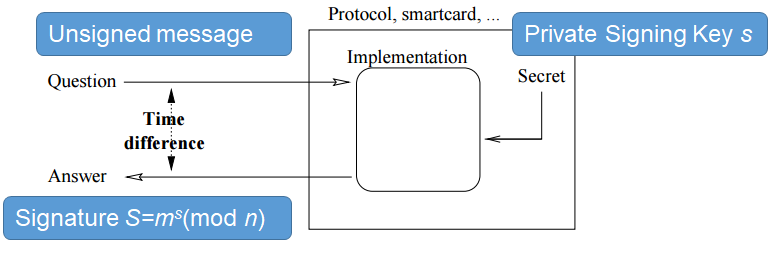
\includegraphics[scale=0.4]{images/smartcard.png}
    \caption{The timing attack principle} \label{fig:smart card}
\end{figure}

So, let's look a bit closer on the attack model - what messages we can send to
the smart card? Can we send any message we want? The answer is that we can only send
valid messages - if the message is not valid then the smart card will just throw 
an exception.
This is somewhere in the scale between the weakest model and the most
powerful model. In this scenario the most permissive attack model is a known plain
text. Known plain text means that we can see the messages as they are go in to the
smart card but cannot change them. So the next thing is choosing the plain text. 
We can't just chose any plain text, it has to follow a certain rule. The next
thing is completely chosen plain text which doesn't enforce any rules, and the
last thing is adaptive plain text which means we can look at the response and we
can choose the next query that we will send. So, what is the attack model, we send
requests, the smart card is signing them, and we get the responses and also
assuming that the smart card is using Montgomery RSA . So how can we use it to
extract the key? We are going to use a method
calles ``Vaizata" method which can be found in the DPA handbook. This is a
general way of performing a side channel attack using statistics. \newline

\underline{The ``Vaizata" Method}
\begin{itemize}
	\item Make a simple assumption about the implementation
	\item Guess a little part of the key
	\item Make hypothesis about the effect of the guess on the execution
	\item Classify the measurements according to the hypothesis
	\item If we guessed right, the classification will be statistically
	meaningful
\end{itemize}

How does it work? First, we make a simple assumption on the implementation, an
assumption could be: We assume that the implementation run on software (the
other possibility is hardware) what does it gives us? Software is executed
serially and in the hardware it's not the case. We can assume for example that
the key is stored in a flash memory on the device, and every time we need to use
the key then we need to read the flash memory. How can we find that this is the
case? How can we find first of all that a device is on using the hardware or the
software? One way is to look at it - we can open the screws and look with a
microscope, or we can go to this wonderful website called ``I fixed it". They
disassemble all sorts of devices and share this information. What is the sign
that the device is using software? If there is an update on the firmware,
because when it wakes up it needs to find out what software to run. We can say
that this device uses memory, and we can also say things about when the 
device is doing the encryption. 
Let's assume the device under test is a remote controller.
Inside the controller there is a secret key stored and also a counter. Whenever
the button is pressed the remote controller constructs a package containing the
serial number of the controller, the counter and a boolean state of the
button (which ever button was pressed). Then, it sends it to a car and the car
decrypts it. Why do we need a serial number? Each ECU in the car has a 
program to accept remote controls. So why do we need the counter? Without the
counter, an attacker can repeat a message sent from the remote controller to the
car only by reading the messages and sending them again. What happens when you
press the button and the car is in the train station? The counter in the remote
controller is out of sync with the counter in the car ans there is a window of
counter values the car will accept. If its closed, the car will open without
complaining. If it's a little closed we will need to press the remote control
twice and when the car will see consecutive values and it will open,
 but if it is too far it won't open. 
 Let's assume we can find out when the controller is
transmitting (it is a very intensive operation that takes battery life and also
radiates). So we know the moment in time when it is transmitting, did the
encryption happened before or after the transmition? The ansewr is before. Let's
assume that the counter stored in the memory and let's say we found the moment in
time when the chip is reading from memory. Did it happen before or after the
encryption? The answer is after, since we need the counter to be included in the
message that will be sent. We can also make more assumptions such as ``the AES
uses an 8 bit data pack or 16 bit or 32 bit". Some of these assumptions might be
wrong but the ``vizata" method will help us to find out if they are wrong. 

So first of all we make a simple assumption, that the smart card is using
left to right binary exponentiation using Montgomery and this is a very
reasonable assumption because most implementations are using this method.
The next thing to do is recursively (or inductively) guess a little part of the key.
if we guessed the whole password it would take us exponential time but if 
we could guess a small part of the key each time it would take a linear time. 
So, we will try to guess small parts of the key first, and maybe the simplest thing 
to explain is guessing one bit or a single character, but lets say we are guessing a small part
of the key. So now we know the beginning of the key and there is a little part
we don't know. The next step is that we need to make a guess about what kind of 
effect our guess is going to have on the computation. We can say, for example,
that if we will guess the bit correctly then something will happen to the
computation, and if we will guess this key bit correctly it will take more
power/take longer time/connect to the network more often or some kind of other 
phenomena we can measure. So, in our case what is the only thing we can measure? Answer:
The anser is time. We assume that if there is a Montgomery reduction in the calculation of
this bit then the entire computation is going to take a little more time.


SO what is going on here? There is a very large computation here and we were able
to guess the beginning of it but not the end of it. Now we are going to classify
the measurements according to our hypothesis, in this case two groups (with or
without Montgomery computation). If we guessed correctly then it will take
longer to the group we said it will take longer. If not, it might take less or
more, we can't detrmine. If we guessed correctly, the groups will have meaning,
means will be able to statistically tell apart the set of the measurements
that will take a longer time and the set of measurements that will take less
time. We are going to guess the left bit of the key, and there is only one option.
The next bit can be 1 or 0. Now, we can
simulate the running of this algorithm with our guess, not for the whole key but only
to the part we know, and if there is going to be Montgomery reduction. So assumeing we
have $g$, $e$ and $N$. The device under test is calculating \(g^emodn\), but where $g$ came
from? It is supplied by the attacker. What about $e$? Secret we want to discover
(\(e_t,e_{t-1},..,e_0\)) What about $N$? public variable (known). The first
thing it does, it enters the Montgomery representation. This information of how
to enter the Montgomery representation is known to the attacker. It starts with
$g$, and then $g$ becomes $Mont(g)$, but the attacker can also do it. First \(A=1\), then
\(A=A*A\) the next thing is \(A=A*g\) because we know that the most significant
bit is 1. The next step is \(A=A*A\), now what is next? It depends, if
\(e_{t-1}\) = 0 then \(A=A*A\) (skipping to next bit). Else if \(e_{t-1}\) = 1
then \(A=A*g\). What happens next now we can't know. We can run both
calculations, in particular we can find out if there was a reduction step in two
optional operations. There are 4 options: Only one of then containing a reduction step,
two of them containing a reduction steo or nither of them. We can know exactly, 
assuming we make a guess on \(e_{t-1}\),
if there is going to be an extra reduction step. We know enough to guess - if we
guess correctly, we can know if there will be a reduction step because we can
calculate all the alternative options completely. So, let's do this now, we have
many different g's, and we have repeated this step many times, and for each of these
g's we know if there is going to be an extra reduction step. So, now let's see
how we can do an attack using this information. So, there is private key $s$, 
a public key $v$ and a signing operation \(m^s mod n\). 

We begin the attack with a bag of messages, all of them are valid, and we send
them to the device under test (DUT). The DUT signs these messages (k messages),
and for each one of the messages we get a trace, which is the data we collected
using the side channel attack in this case it is only the time. Now we have a
vector of size k and each element in the vector is the time it took to sign the
message. Now, we are going to try and guess \(s_t,s_{t-1}\) \((s =
s_t,s_{t-1},s_{t-2},…,s_0)\) and try to discover \(s_{t-2}\). 

So for each of the messages and each key guess we are going to simulate the
computation as far as we already know and in addition for the parts of the key
that we don't know we are going to simulate twice - one with a 0 and one with a
1. We are going to find out where the extra reduction step happens. If the next
bit is 0, then some of the messages have extra reduction and we classify the message into
two bins, those who got extra reduction and those who didn't. But maybe the key
is not 0? maybe its 1. So we can simulate the same thing with the next bit as 1,
and find out different set of messages with an extra reduction step. We can't
find what the bits are but we can make a guess and simulate on both 0 and 1. So,
now we divide our traces into two groups in 2 different ways, if the next key
bit is 0 then \(m_1,m_2,m_4,m_5,m_7\) got extra reduction and \(m_3,m_6,m_8,m_9\)
didn't. If the next key bit is 1 then \(m_2,m_3,m_5,m_8\) got extra reduction and
\(m_1,m_4,m_6,m_7,m_9\) didn't (see \Cref{fig:extraRed}). 


\begin{figure}[!ht]
    \centering
    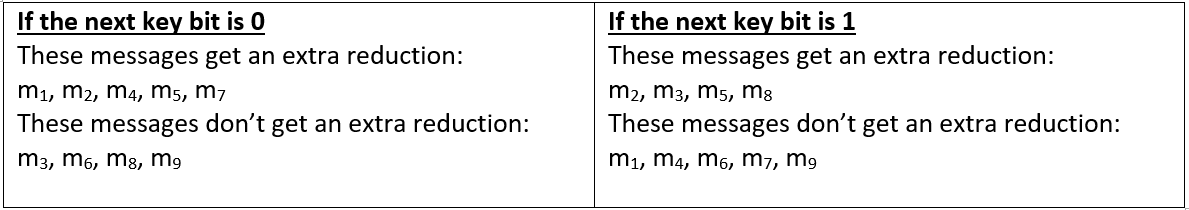
\includegraphics[scale=0.3]{images/extraRed.PNG}
    \caption{Key bit guess simulation} \label{fig:extraRed}
\end{figure}

If we guessed correctly what can we tell about the messages that got an extra
reduction? Their runtime will be a little longer if we guessed the key bit
correctly and If we guessed incorrectly it means we divided into two random
groups which means the runtime will be similar in both groups. So if we guessed
correctly the difference in runtime between the groups will be measurably
different. So now we are going to change the discussion about the messages into
the traces.

\begin{figure}[!ht]
    \centering
    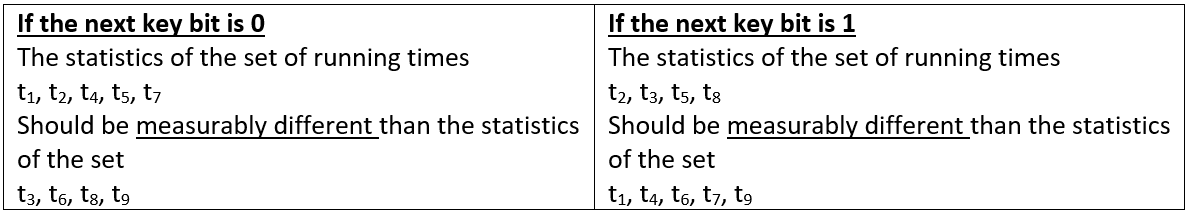
\includegraphics[scale=0.3]{images/extraStat.PNG}
    \caption{Guessing correctly the key bit makes the statics measurably different} \label{fig:extraStat}
\end{figure}


if the next key bit is 0 then the statistics of the runtimes of 0 bit with extra
reduction are going to be different from the runtimes of 0 bit without extra
reduction. If we were wrong then the runtimes of 1 bit with extra reduction will
be different from 1 bit without the extra reduction. Notice that we are not saying
average or mean anywhere, because they are not required, it could be the
variance changes or something else. The point is that there is some kind of
difference that we can measure. So, how can we find out which of these two
divisions is the correct one? Answer: we have two divisions of k traces and we
measure the distance of the means. We are going to calculate the mean runtime of each
part (0 bit with or without the extra reduction and 1 bit with or without the
extra reduction) and subtract between with/without extra reduction in each bit
guess. If there is a large distance of means of the 0 bit guess as oppose to the
1 bit guess then probably the splitting of traces in the 0 bit guess is more
meaningful than the 1 bit guess. If we are able to split meaningfully then we
guessed the key correctly. Now, let's go back into statistics and talk about the
T-test~\cite{wikittest}. The T-test was invented by William Sealy
Gosset~\cite{wikigosset} who was a chemist who worked for a very famous brewery
in Ireland (Guinness). So, what is the idea? We have two populations that are
different in some way. There are two kinds of t-tests, pair T-test and unpaired
T-test. what is the paired T-test? lets assume we are going to a
tree and we taking the leaves that fall off the tree. We notice that the leaves
that fall on the south side have less mold that the leaves that fall
on the north side. Why is that? Because there is more sun on the south side that
is drying the leaves. 

How do we prove our theory? We send our undergrad research assistant to collect
a bag of leaves form the north side and a bag of leaves from the south side and 
tell the undergrad to count the percentage of mold in the southern and northern
leaves. When the undergrad comes back, very exhausted, he provides us with an
excel file that have 1000 leaves from the north side and 1500 from the south
side. Now we want to prove our theory, each one of the leaves has a mold, We
want to prove that there is a statistical difference between the two groups - 
this is the unpaired T-test. What is the paired T-test? 
It is when we are talking about
something which we can identify as pairs. For example, we are developing a
cancer medicine and we want to test it. Now, we don't take any undergrads but
only very sick mice with cancer. We measure the weight of the tumor in order to
have a list of 100 mice and tumors. Then we divide them into two groups, one we
treat with a medicine and the other we don't. In the end of the experiment, we
measure the tumors again, but now each measurement is a pair, one before the
treatment and one is after. We want to say that the size of the tumor is
smaller after the treatment. Now let's review the student's unpaired T-test demo
in Matlab. The mat in Matlab is for matrix, we can define matrix like this:

\begin{figure}[!ht]
    \centering
    \fbox{
    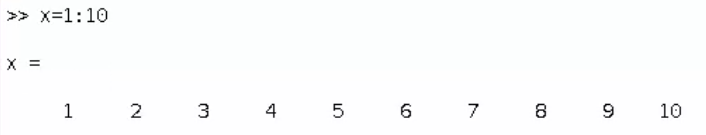
\includegraphics[scale=0.5]{images/defmat.png}}
    \caption{Defining a matrix of size 1x10 with increasing numbers from 1 [1,2,3,…,10]} \label{fig:defmat}
\end{figure}

\begin{figure}[!ht]
    \centering
    \fbox{
    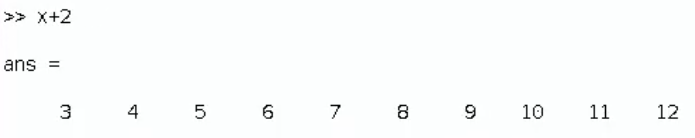
\includegraphics[scale=0.5]{images/defmat2.png}}
    \caption{Adding the matrix with 2 increases all the numbers in the matrix by 2 (Same with multiplication and log)} \label{fig:defmat2}
\end{figure}

\begin{figure}[!ht]
    \centering
    \fbox{
    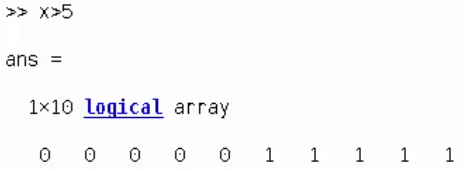
\includegraphics[scale=0.5]{images/defmat3.png}}
    \caption{\(x>5\) will result with logical array [0, 0, 0, 0…, 1, 1, 1, 1]} \label{fig:defmat3}
\end{figure}

The function randn(1) which creates normally distributed random variable which
follows a Gaussian distribution which means the variance is 1 and the mean of 0.
What is the minimum value this function will output? Answer: None, but
statistically the value is closer to 0. How can we create a random variable with
mean different from 0? Answer: add a constant to the mean, if we want mean N. we will do $N$ +
randn (1). We can even create a vector of randomly chosen numbers using randn
(1, 5) + 5 : [4.9369, 5.7147, 4.7950, 4.8759, 6.4897] and if we will do randn
(1, 5)*.1 + 5 the numbers will be even closer to 5. So, now we are ready to try
the student T-test.

\begin{figure}[!ht]
    \centering
    \fbox{
    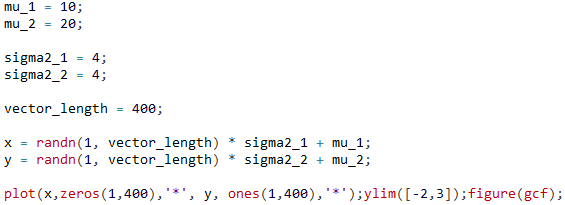
\includegraphics[scale=0.6]{images/defmat4.png}}
    \caption{In the code, 2 vectors are created - x and y in the same size (which is not obligatory), $x$ will be randomly distributed with a mean of \(mu_{1}\) and variance of \(sigma2_1\) and vector $x$ is going to be random distributed with a mean of \(mu_2\) and variance of \(sigma2_2\). Then there is a code for plotting both vectors (in different colors).} \label{fig:defmat4}
\end{figure}

\begin{figure}[!ht]
    \centering
    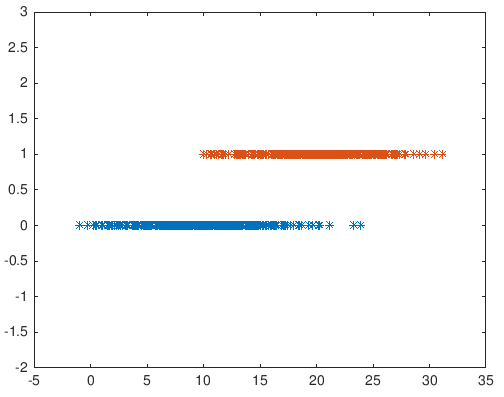
\includegraphics[scale=0.6]{images/defmatplot.png}
    \caption{Plotting of the vectors for \(mu_1 = 10, mu_2 = 20\)} \label{fig:defmatplot}
\end{figure}

Looking only on the graphs - can we say they are from the same distribution?
Answer: we can't be sure. We want to run the T-test to find out if they are
statistically significant. There is a hypothesis and we need to either reject or
accept the hypothesis. If \(H_0\) then they are from the same distribution and
if \(H_1\) than they are from different distributions. If we run the code, the
result will be that they are from different distributions with 0.959 certainty.
Each time we run we can get different results, if the certainty is smaller than
0.95, the hypothesis is rejected. How can we make it more difficult
for the ttest2? Answer: if we change \(mu_2\) to 11, then they will be very
close distributions. 

\begin{figure}[!ht]
    \centering
    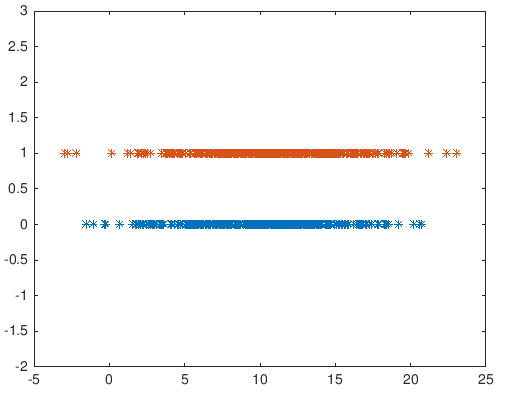
\includegraphics[scale=0.6]{images/defmatplot2.png}
    \caption{Plotting of the vectors for \(mu_1 = 10, mu_2 = 11\)} \label{fig:defmatplot2}
\end{figure}

How we as attackers can handle this situation? Answer: run many times. So we
change the vector length (for example to 50000). There is something called power
analysis, which means given these parameters ($mu$ and $sigma$) how many
measurements you need to run to be sure with 95 percent. As engineers we don't really
care about T-tests, we have a budget of measurements and we just take the one
with the larger mean distance, but what if we are wrong (guessed 1 instead of
0)? After we guessed one bit wrong all the bits afterwards are wrong
because they are simulated wrongly. So, how can we simulate a full attack? If we
guessed 1 bit using the differences of means then we continue to the next bit in
linear time. Let's review a figure from " A Practical Implementation of the
Timing Attack" which you are encouraged to read.


\begin{figure}[!ht]
    \centering
    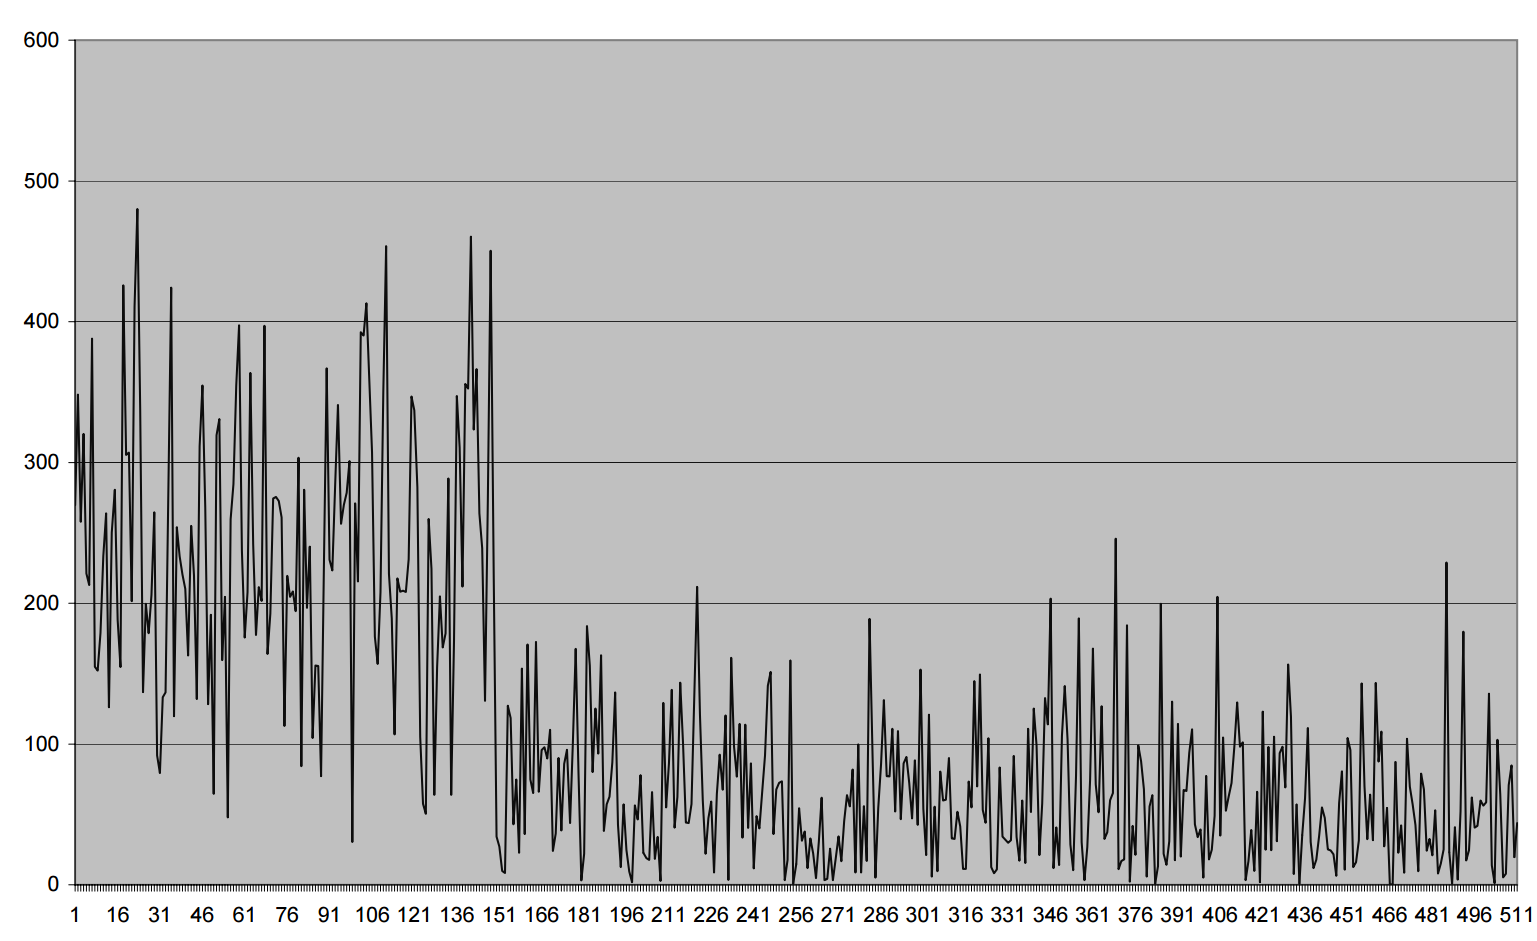
\includegraphics[scale=0.25]{images/figpita.png}
    \caption{x axis – is the bit index from right to left (the left most bit is known to be 1) and y axis – is the distance of means we chose (some times its 500 or 100 but after 151 the distance of means is a lot smaller which means we guessed a bit wrong). How to solve it? Answer: go backwards and backtrack.} \label{fig:figpita}
\end{figure}

Now let's talk about counter measurements. When Kocher announced the attack to
the cipherpunks mailing list there was kind of discussion about it. Here is a
message (see \Cref{fig:paul}) from there that was sent by Ron Riverst. He was
replying to William Simpson, who was the author of Photuris which is related to
the IPsec protocol and was used for kits change in the IP protocol. 

\begin{figure}[!ht]
    \centering
    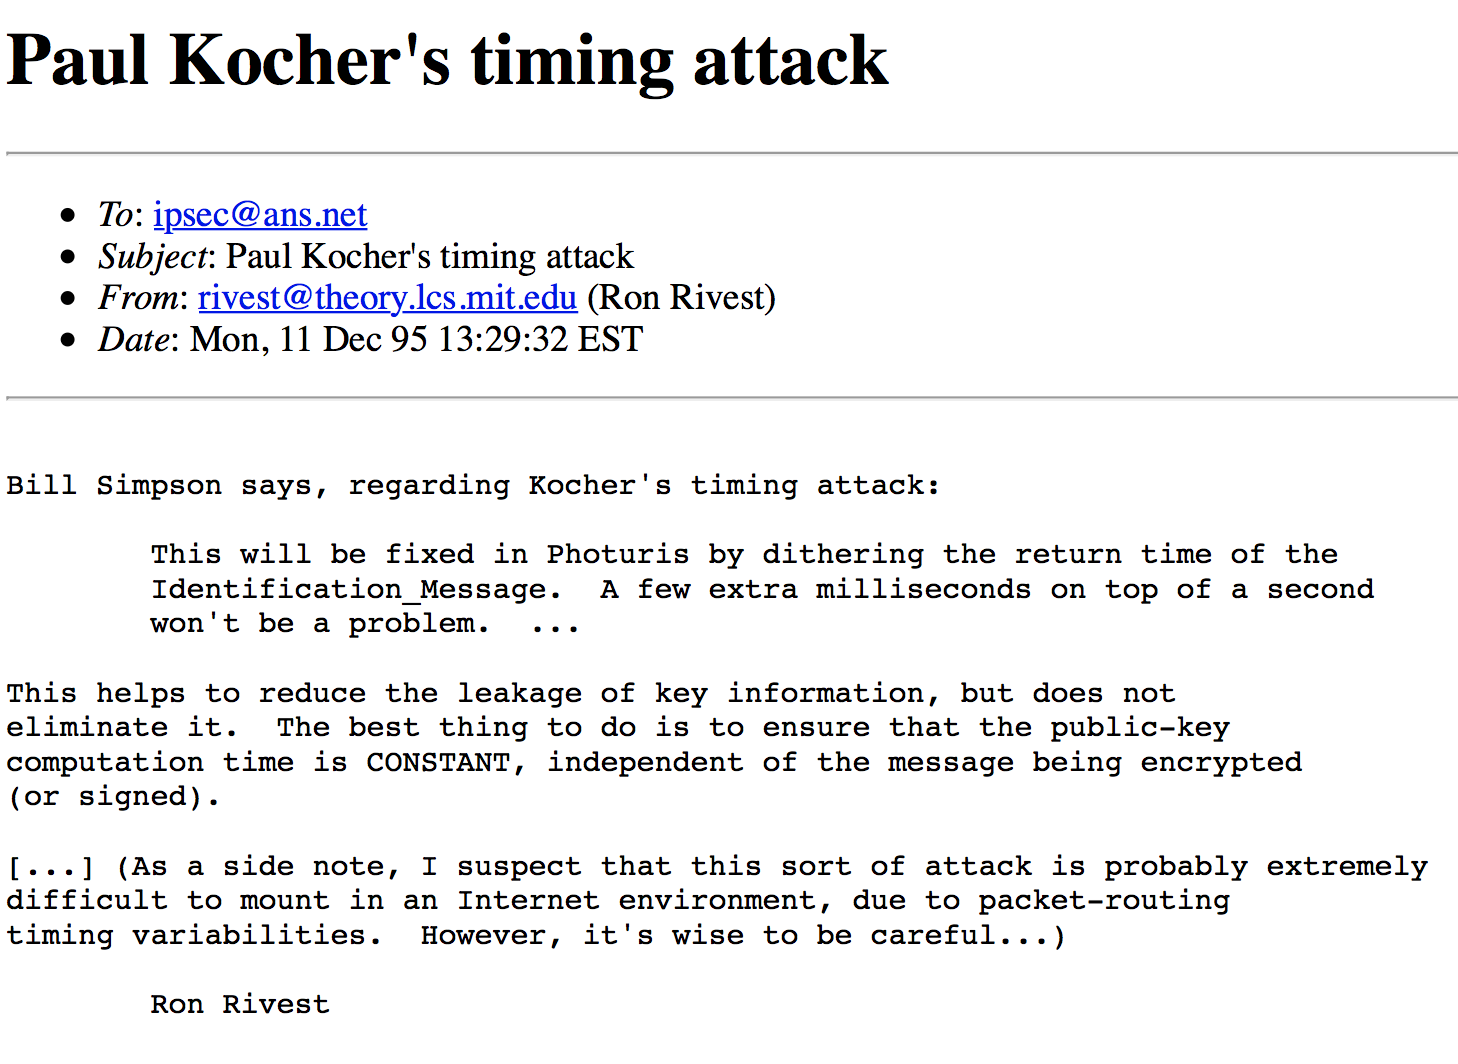
\includegraphics[scale=0.25]{images/paul.png}
    \caption{The message.} \label{fig:paul}
\end{figure}

When he read that this attack can attack Photuris, Bill replied: don't worry
this will be fixed in Photuris. How to do this? By dithering the return time of
identification message a few extra milliseconds. Which means he is doing
mitigation, as he is not adding a random delay because random is very expensive, he
is going to finish the calculations and is going to look at the clock and
exactly when the millisecond changes (or second) send the package. What does it
mean? It means that since the beginning is random then he is going to add a random
delay. So, what Ron Rivest replied? It will reduce the data leakage but will not
eliminate it. Why so? How the attacker will overcome this? He will need
to measure more, this is network-based protocol, the attacker can measure as 
many times as he wants. He says, in addition, the public key computation time should be
constant and independent from the message being sent. Ron Rivest suggest
prevention as a countermeasure. So, what time it is going to be? Answer: the
worst-case time. he adds a side note that this kind of attack is very difficult
to mount in an internet environment due to packet-routing timing variabilities,
however it is wise to be careful. Few years later a demonstration was presented
over the internet, there were more measurements to counter the routing problem.
Adding noise is sometimes the only thing that works, if you add enough noise to
delay the attack time up to a year the message might not be relevant by the time the attack succeeds.

So, let's talk about two more counter measurements, which are preventions. The first
one is called RSA blinding. RSA blinding is a prevention counter measure which
actually works on average time and not on worst-case time. if we have a secret key $S$ and
want to calculate \(m^s mod n\), and the attacker gives us $m$ and we don't want
to leak $s$. We showed that with enough attempts from the attacker he will eventually
retrieve $s$. 

So, how do we do blinding? First of all, we can do this even before the attacker
arrives, we generate random $r$ and calculate \(r^v mod n\) and \(r^{-1} mod
n\). These calculations are not reviling any secrets because $v$ is the public
key. The attacker gives us $m$, so we calculate: 

\[X = (r^v * m) mod n\]
\[Y = X^s = (r^v*m)^s = r^{vs}*m^s = r*m^s mod n \] 
\[ // v*s mod n = 1 mod n)\]

Now, $Y$ is leaking information because we raise a number to the power of the
secret key, but $r$ is a random number which the attacker doesn't know so he can't
simulate the execution. How we remove $r$? We just calculate 

\[S = Y*r^{-1} = r*m^s*r^{-1} = m^s mod n\]

Why doesn't everybody use it? Answer: because it's expensive, 2 modular
exponentiations instead of 1. Another problem is the random number generation,
its hard to find random number generator. You can see RSA blinding in openPGP. 

Now let's review another countermeasure. It called square and always multiply
(see \Cref{fig:saama}). It is very similar to the square and multiply, just
instead of only when \(d_i\) is 1 we will always calculate the multiply but the
assignment will be only when \(d_i\) is 1. The problem with this is not the
extra computation that came from turning sometimes to always. Speculative
execution is always looking for instruction to execute, how does it decide if it
will execute an instruction? If all it's dependencies are met. If I say \(a =
b*c\) and \(e = b*c\) they can run both in the same time. What happens is when
the instruction brought to the CPU there is actually nobody is waiting for $t$, so
as soon as it finishes to run the \(s =s *s mod n\) and \(d_i\) is equal to 0 it
will just return $s$. Moreover, the compilers are also capable of detecting such
cases and optimize them by dismissing the else statement. So if we have a very
simple CPU with no speculative execution no compiler and we wrote it in assembly
we won't be able to attack it, but we could use power analysis.

\begin{figure}[!ht]
    \centering
    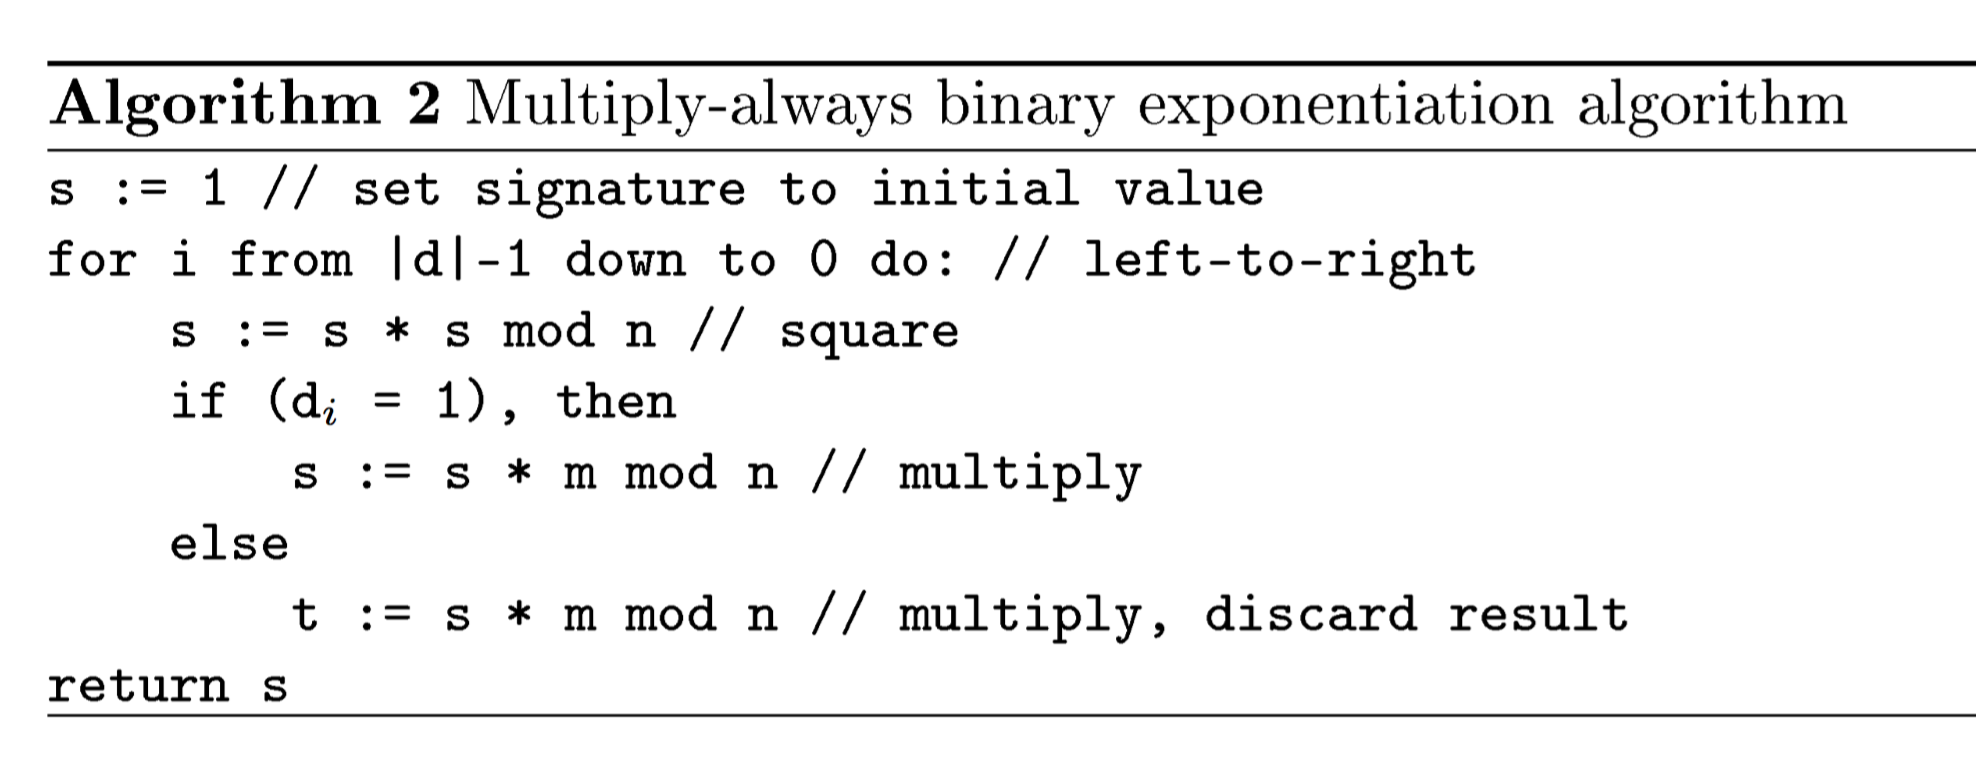
\includegraphics[scale=0.15]{images/saama.png}
    \caption{Square and always multiple algorithm} \label{fig:saama}
\end{figure}

If we run this algorithm as is, we have two places in memory for $s$ and for $t$,
every action we load $s$ then multiply and then edit the memory of $s$. Same goes in
the multiply section. We load $s$ and $m$ and then multiply and store it in $s$. It's
always loading and storing $s$, but what happens when it goes to the else statment:
it loads $s$ and $m$ and then store this into something other then $s$. So the power
consumption is different between the store and the load. You can read more in
the paper (``defeating RSA multiply-always and message binding" by Marc F.
Witteman et al.~\cite{witteman2011defeating})

Side channel attacks can get not only computer secrets but human secrets too.
What exactly is a human secret? Browsing history for example. How does the
website figure out our browsing history? Theoretically, we can delete the
history in the browser. But what happens when we click on a hyper link (blue
link)? It turns purple after the click. So, there was a nice trick that websites
used to do, they attached the link to an HTML element and added JavaScript code
that at the change of the color can now update that you have visited the site.
The world wide web consortium decided that it was a privacy leak and you are not
allowed to read the color of an HTML element anymore. Now we can set the color
but can't read it. One of the speakers in the black hat 2013 used timing attacks
to find out if a web site was visited or
not\footnote{\url{https://www.youtube.com/watch?v=KcOQfYlyIqw}}. He also
demonstrated how he can also use timing attack to read the user's stream. 
\section{Research highlights} \label{sec:RelatedWork}
\begin{itemize}
    \item \textbf{Photonic Side Channel Attacks Against RSA} - This paper describes an attack utilizing the
    photonic side channel against a public-key crypto-system. They
    evaluated three common implementations of RSA modular exponentiation, all using the Karatsuba multiplication method.
    It was discovered that the key length had marginal impact on resilience to the attack.
    They noticed that the most dominant parameter impacting the attacker’s effort is the minimal block size at which the Karatsuba method reverts to naive multiplication.
    They also discovered that Montgomery’s Ladder was actually the most susceptible to the attack.
    \href{https://www.eng.tau.ac.il/~yash/ieee-host-2017.pdf}{Photonic Side Channel Attacks Against RSA}.
\end{itemize}

\chapter{Power/EM I} \label{c4_forthchapter:cha}

\section{Electronic Circuits}

\subsection{A basic electronic circuit}

The most basic electronic circuit consist of a power supply (i.e. a battery)
that generates an electric potential that aim to move to the ground. And an
electrical load (any component consuming electric power) connected to the power
supply (Vdd) on one side and to the ``ground" (the reference point from which
voltages are measured) on the other side. As the electric potential goes through
the load, it (the load) does some kind of a work. We can consider electric
current to behave like water, in this example the water wants to go from the
mountains (Vdd) to the sea level (Ground) and there are rivers and obstacles
that tries to prevent it to do so. When the load has small resistance then more
of the current will “flow” through it, and when the load has bigger resistance
then the “flow” is smaller.

There are two different ways in which we can wire things together in an electric
circuit, called series and parallel. When things are wired in series, things are
wired one after another, such that electricity has to pass through one load,
then the next load, then the next, and so on. When things are wired in parallel,
they are wired side by side, such that electricity passes through all of them at
the same time, from one common point to another common point. The difference in
the electric potential between the power supply and the ground creates an
electric current which flows through the load toward the ground. The difference
in electric potential between two points is measured in Volts (usually denoted
by \textbf{\textit{V}}). The amount of current flowing through the circuit at a
given time is measured in Amperes (denoted by \textbf{\textit{A}}). The
electrical resistance of the load is a measure of its opposition to the flow of
electric current through it. It is measured in Ohms (and denoted by
\textbf{\textit{R}}).


\begin{figure}[!ht]
	\centering
	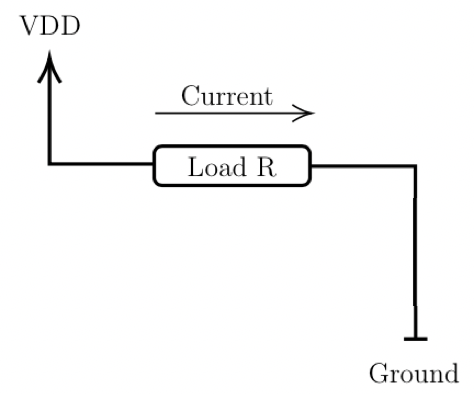
\includegraphics{images/basic_electronic_circuit.png}
	\caption{Basic electronic circuit.} \label{fig:basic_electronic_circuitn}
\end{figure}

\subsection{Resistors}

As the name implies, a resistor resists the flow of electrical current. The
amount of resistance is measured in Ohms. A resistor is considered a passive
component that consumes power that is dissipated as heat. The power rating of a
resistor determines how much power it can consume without overheating.

\begin{figure}[!ht]
    \centering
    \tikzset{every picture/.style={line width=0.75pt}} %set default line width to 0.75pt        

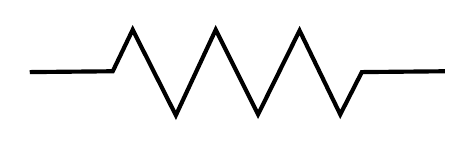
\begin{tikzpicture}[x=0.75pt,y=0.75pt,yscale=-1,xscale=1]
%uncomment if require: \path (0,82); %set diagram left start at 0, and has height of 82

%Straight Lines [id:da11666992549989796] 
\draw [line width=1.5]    (11.4,40.02) -- (51.4,39.62) -- (61,19.62) -- (81.8,60.82) -- (101,19.62) -- (121.4,60.42) -- (141.4,20.02) -- (161,60.42) -- (171.4,40.02) -- (211.4,39.62) ;






\end{tikzpicture}
    \caption{Resistor Symbol in Circuit Diagrams.} \label{fig:resistor}
\end{figure}

\subsection{Ohm's law}

\begin{figure}[!ht]
	\centering
	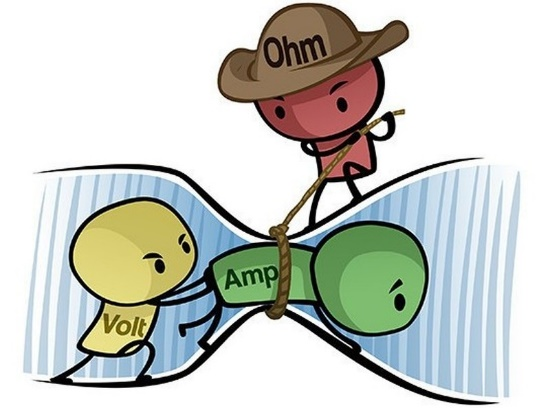
\includegraphics{images/ohms_law_cartoon.png}
	\caption{Ohm's Law.} \label{fig:ohms_law_cartoon}
\end{figure}

Ohm's law defines the relationship between the Voltage, Current and Resistance
in a circuit: The voltage is equal to the current multiplied by the resistance
of the load. 

\begin{displaymath}\label{eq:ohm}
    V=I*R
\end{displaymath}

Since in most of the circuits we are using, the voltage is fixed (defined by the
characteristics of the power supply), a change in the resistance of the circuit
will cause a change in the current in the opposite direction. This means we can
measure the current over time in order to calculate the resistance. A useful
analogy for the relations between V, I and R is to imagine a fountain on a high
mountain, where the water flow down through a river to the sea. The difference
in height between the fountain and the sea is the Voltage, the width of the
river can be thought of as the resistance, and the flow of the water is the
current.

\subsection{Power}

Power is the rate at which work is done by the circuit and is measured in Watts.
Electricity bills are measured by K Watts hour, i.e. 1 KWH is 1 kilo watts used
over an hour, and this is the energy that we used and we need to pay for. $Power
= Work / Time$

\begin{displaymath}\label{eq:power_consumption}
    \textrm{Power consumption:} P=I*V
\end{displaymath}

For example we can take a look on a phone; the battery can be measure in
Milliamper hour, i.e. if the battery is 3000mil Amper Hour so if the current is
1 Amper then we can use it for 3 hours. If we want the battery to run out
quickly, we can use services like streaming, flashlight and more. That means we
have greater current that caused by leveraging the load of the phone and the
battery will run our much faster than before. The phone also, will get hot. If a
device is getting hot then it sometimes uses its fans (noise), and so we can
detect it for cyber usage.

Electricity can be used to do various kinds of work:
\begin{itemize}
    \item Electromagnetic work (light a bulb, transmit a Wi-Fi signal)
    \item Thermal work (heating)
    \item Mechanical work (spin a motor, vibrate a speaker)
    \item Chemical work (charging a battery)
    \item Computational work (store or load from memory, compute a value)
\end{itemize}

\subsection{Power Consumption}

When the current leaves the circuit to the ground then we consume it as power,
but sometimes we need to be careful as there are cases where the current is no
leaving the circuit, like battery charging. In order to measure the power we
will connect our measuring device between the load and the ground. The power
consumption of a device is the work it does divided by time. It is measured in
Watts (\textbf{\textit{W}}). The power consumption can be calculated as current
(\textbf{\textit{I}}) multiplied by Voltage (\textbf{\textit{V}}).

\subsection{Current and Voltage dividers}

Before we take a look at two simple electronic circuits, we need to introduce
two additional terms: A \textbf{short (closed) circuit} is a piece of wire with
almost no resistance at all. The circuit is in a closed state and there is
current in the circuit. In other words, it works as normal. An \textbf{open
circuit} is a circuit which doesn't allow any current to pass through it. The
circuit is in an open state and there is no current in the circuit; that's to
say. It doesn't work.

\begin{figure}[!ht]
    \centering
    

\tikzset{every picture/.style={line width=0.75pt}} %set default line width to 0.75pt        

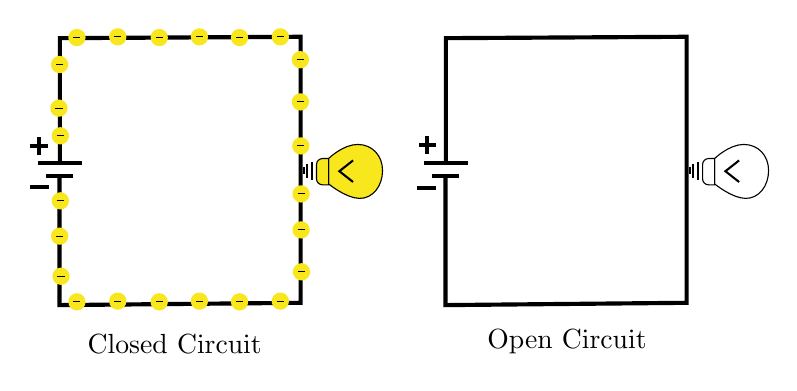
\begin{tikzpicture}[x=0.75pt,y=0.75pt,yscale=-1,xscale=1]
%uncomment if require: \path (0,199.3333282470703); %set diagram left start at 0, and has height of 199.3333282470703

%Straight Lines [id:da2325261898014528] 
\draw [color={rgb, 255:red, 0; green, 0; blue, 0 }  ,draw opacity=1 ][line width=1.5]    (35.5,90.67) -- (35.5,152.67) -- (151.67,151.56) -- (151.67,23.39) -- (35.67,24.06) -- (35.67,84.06) ;

\draw [shift={(35.5,90.67)}, rotate = 270] [color={rgb, 255:red, 0; green, 0; blue, 0 }  ,draw opacity=1 ][line width=1.5]    (0,6.71) -- (0,-6.71)   ;
%Straight Lines [id:da28409341931115617] 
\draw [color={rgb, 255:red, 0; green, 0; blue, 0 }  ,draw opacity=1 ][line width=1.5]    (25,84.06) -- (46.33,84.06) ;


%Shape: Polygon Curved [id:ds5857087256403513] 
\draw  [fill={rgb, 255:red, 248; green, 231; blue, 28 }  ,fill opacity=1 ] (165.14,94.26) .. controls (165.14,94.26) and (173.39,101.09) .. (179.94,101.26) .. controls (186.5,101.42) and (191.14,95.16) .. (191.14,87.86) .. controls (191.15,80.56) and (186.14,75.26) .. (179.14,75.26) .. controls (172.14,75.26) and (165.12,82.03) .. (165.14,82.06) .. controls (165.17,82.08) and (165.14,94.26) .. (165.14,94.26) -- cycle ;
%Rounded Same Side Corner Rect [id:dp42554815939285007] 
\draw  [fill={rgb, 255:red, 248; green, 231; blue, 28 }  ,fill opacity=1 ] (162.24,94.72) .. controls (160.63,94.72) and (159.33,93.42) .. (159.33,91.82) -- (159.33,84.96) .. controls (159.33,83.36) and (160.63,82.06) .. (162.24,82.06) -- (165.14,82.06) .. controls (165.14,82.06) and (165.14,82.06) .. (165.14,82.06) -- (165.14,94.72) .. controls (165.14,94.72) and (165.14,94.72) .. (165.14,94.72) -- cycle ;
%Straight Lines [id:da9150604099279609] 
\draw [line width=0.75]    (156.94,83.96) -- (156.94,92.56) ;


%Straight Lines [id:da28384528220983696] 
\draw [line width=0.75]    (154.94,84.76) -- (154.94,91.56) ;


%Straight Lines [id:da8752324892632142] 
\draw [line width=0.75]    (153.34,86.36) -- (153.34,89.56) ;


%Straight Lines [id:da25290786107493535] 
\draw [line width=0.75]    (176.94,82.96) -- (170.34,88.16) -- (176.94,93.36) ;


%Straight Lines [id:da9185196513242853] 
\draw [line width=1.5]    (21.17,95.78) -- (30.5,95.78) ;


%Shape: Circle [id:dp23397738064818174] 
\draw  [draw opacity=0][fill={rgb, 255:red, 248; green, 231; blue, 28 }  ,fill opacity=1 ] (147.6,75.97) .. controls (147.6,73.67) and (149.47,71.8) .. (151.77,71.8) .. controls (154.07,71.8) and (155.93,73.67) .. (155.93,75.97) .. controls (155.93,78.27) and (154.07,80.13) .. (151.77,80.13) .. controls (149.47,80.13) and (147.6,78.27) .. (147.6,75.97) -- cycle ;
%Straight Lines [id:da482836286674198] 
\draw    (150.05,75.97) -- (153.48,75.97) ;



%Shape: Circle [id:dp7549375095754003] 
\draw  [draw opacity=0][fill={rgb, 255:red, 248; green, 231; blue, 28 }  ,fill opacity=1 ] (147.4,54.77) .. controls (147.4,52.47) and (149.27,50.6) .. (151.57,50.6) .. controls (153.87,50.6) and (155.73,52.47) .. (155.73,54.77) .. controls (155.73,57.07) and (153.87,58.93) .. (151.57,58.93) .. controls (149.27,58.93) and (147.4,57.07) .. (147.4,54.77) -- cycle ;
%Straight Lines [id:da4285424058101477] 
\draw    (149.85,54.77) -- (153.28,54.77) ;



%Shape: Circle [id:dp5457818708688953] 
\draw  [draw opacity=0][fill={rgb, 255:red, 248; green, 231; blue, 28 }  ,fill opacity=1 ] (147.4,34.43) .. controls (147.4,32.13) and (149.27,30.27) .. (151.57,30.27) .. controls (153.87,30.27) and (155.73,32.13) .. (155.73,34.43) .. controls (155.73,36.73) and (153.87,38.6) .. (151.57,38.6) .. controls (149.27,38.6) and (147.4,36.73) .. (147.4,34.43) -- cycle ;
%Straight Lines [id:da8515924061724973] 
\draw    (149.85,34.43) -- (153.28,34.43) ;



%Shape: Circle [id:dp4359422667224846] 
\draw  [draw opacity=0][fill={rgb, 255:red, 248; green, 231; blue, 28 }  ,fill opacity=1 ] (137.73,23.43) .. controls (137.73,21.13) and (139.6,19.27) .. (141.9,19.27) .. controls (144.2,19.27) and (146.07,21.13) .. (146.07,23.43) .. controls (146.07,25.73) and (144.2,27.6) .. (141.9,27.6) .. controls (139.6,27.6) and (137.73,25.73) .. (137.73,23.43) -- cycle ;
%Straight Lines [id:da45892746068057066] 
\draw    (140.19,23.43) -- (143.61,23.43) ;



%Shape: Circle [id:dp10968014625901534] 
\draw  [draw opacity=0][fill={rgb, 255:red, 248; green, 231; blue, 28 }  ,fill opacity=1 ] (118.07,23.77) .. controls (118.07,21.47) and (119.93,19.6) .. (122.23,19.6) .. controls (124.53,19.6) and (126.4,21.47) .. (126.4,23.77) .. controls (126.4,26.07) and (124.53,27.93) .. (122.23,27.93) .. controls (119.93,27.93) and (118.07,26.07) .. (118.07,23.77) -- cycle ;
%Straight Lines [id:da5692830288753206] 
\draw    (120.52,23.77) -- (123.95,23.77) ;



%Shape: Circle [id:dp43116716627713836] 
\draw  [draw opacity=0][fill={rgb, 255:red, 248; green, 231; blue, 28 }  ,fill opacity=1 ] (98.73,23.43) .. controls (98.73,21.13) and (100.6,19.27) .. (102.9,19.27) .. controls (105.2,19.27) and (107.07,21.13) .. (107.07,23.43) .. controls (107.07,25.73) and (105.2,27.6) .. (102.9,27.6) .. controls (100.6,27.6) and (98.73,25.73) .. (98.73,23.43) -- cycle ;
%Straight Lines [id:da7403562369362462] 
\draw    (101.19,23.43) -- (104.61,23.43) ;



%Shape: Circle [id:dp03302036024104882] 
\draw  [draw opacity=0][fill={rgb, 255:red, 248; green, 231; blue, 28 }  ,fill opacity=1 ] (79.4,23.77) .. controls (79.4,21.47) and (81.27,19.6) .. (83.57,19.6) .. controls (85.87,19.6) and (87.73,21.47) .. (87.73,23.77) .. controls (87.73,26.07) and (85.87,27.93) .. (83.57,27.93) .. controls (81.27,27.93) and (79.4,26.07) .. (79.4,23.77) -- cycle ;
%Straight Lines [id:da40757318650872465] 
\draw    (81.85,23.77) -- (85.28,23.77) ;



%Shape: Circle [id:dp8000122366529838] 
\draw  [draw opacity=0][fill={rgb, 255:red, 248; green, 231; blue, 28 }  ,fill opacity=1 ] (59.4,23.43) .. controls (59.4,21.13) and (61.27,19.27) .. (63.57,19.27) .. controls (65.87,19.27) and (67.73,21.13) .. (67.73,23.43) .. controls (67.73,25.73) and (65.87,27.6) .. (63.57,27.6) .. controls (61.27,27.6) and (59.4,25.73) .. (59.4,23.43) -- cycle ;
%Straight Lines [id:da0875021467717878] 
\draw    (61.85,23.43) -- (65.28,23.43) ;



%Shape: Circle [id:dp05690070919084467] 
\draw  [draw opacity=0][fill={rgb, 255:red, 248; green, 231; blue, 28 }  ,fill opacity=1 ] (39.73,23.77) .. controls (39.73,21.47) and (41.6,19.6) .. (43.9,19.6) .. controls (46.2,19.6) and (48.07,21.47) .. (48.07,23.77) .. controls (48.07,26.07) and (46.2,27.93) .. (43.9,27.93) .. controls (41.6,27.93) and (39.73,26.07) .. (39.73,23.77) -- cycle ;
%Straight Lines [id:da5744558280008554] 
\draw    (42.19,23.77) -- (45.61,23.77) ;



%Shape: Circle [id:dp09815936705452866] 
\draw  [draw opacity=0][fill={rgb, 255:red, 248; green, 231; blue, 28 }  ,fill opacity=1 ] (31.4,36.77) .. controls (31.4,34.47) and (33.27,32.6) .. (35.57,32.6) .. controls (37.87,32.6) and (39.73,34.47) .. (39.73,36.77) .. controls (39.73,39.07) and (37.87,40.93) .. (35.57,40.93) .. controls (33.27,40.93) and (31.4,39.07) .. (31.4,36.77) -- cycle ;
%Straight Lines [id:da1455188221370589] 
\draw    (33.85,36.77) -- (37.28,36.77) ;



%Shape: Circle [id:dp898572524230915] 
\draw  [draw opacity=0][fill={rgb, 255:red, 248; green, 231; blue, 28 }  ,fill opacity=1 ] (31.07,57.77) .. controls (31.07,55.47) and (32.93,53.6) .. (35.23,53.6) .. controls (37.53,53.6) and (39.4,55.47) .. (39.4,57.77) .. controls (39.4,60.07) and (37.53,61.93) .. (35.23,61.93) .. controls (32.93,61.93) and (31.07,60.07) .. (31.07,57.77) -- cycle ;
%Straight Lines [id:da9743601868292349] 
\draw    (33.52,57.77) -- (36.95,57.77) ;



%Shape: Circle [id:dp6955964743895362] 
\draw  [draw opacity=0][fill={rgb, 255:red, 248; green, 231; blue, 28 }  ,fill opacity=1 ] (31.73,71.1) .. controls (31.73,68.8) and (33.6,66.93) .. (35.9,66.93) .. controls (38.2,66.93) and (40.07,68.8) .. (40.07,71.1) .. controls (40.07,73.4) and (38.2,75.27) .. (35.9,75.27) .. controls (33.6,75.27) and (31.73,73.4) .. (31.73,71.1) -- cycle ;
%Straight Lines [id:da6213610339187869] 
\draw    (34.19,71.1) -- (37.61,71.1) ;



%Shape: Circle [id:dp9264817359074005] 
\draw  [draw opacity=0][fill={rgb, 255:red, 248; green, 231; blue, 28 }  ,fill opacity=1 ] (137.73,150.77) .. controls (137.73,148.47) and (139.6,146.6) .. (141.9,146.6) .. controls (144.2,146.6) and (146.07,148.47) .. (146.07,150.77) .. controls (146.07,153.07) and (144.2,154.93) .. (141.9,154.93) .. controls (139.6,154.93) and (137.73,153.07) .. (137.73,150.77) -- cycle ;
%Straight Lines [id:da9036669479861532] 
\draw    (140.19,150.77) -- (143.61,150.77) ;



%Shape: Circle [id:dp5844969098724175] 
\draw  [draw opacity=0][fill={rgb, 255:red, 248; green, 231; blue, 28 }  ,fill opacity=1 ] (118.07,151.1) .. controls (118.07,148.8) and (119.93,146.93) .. (122.23,146.93) .. controls (124.53,146.93) and (126.4,148.8) .. (126.4,151.1) .. controls (126.4,153.4) and (124.53,155.27) .. (122.23,155.27) .. controls (119.93,155.27) and (118.07,153.4) .. (118.07,151.1) -- cycle ;
%Straight Lines [id:da09046684668382188] 
\draw    (120.52,151.1) -- (123.95,151.1) ;



%Shape: Circle [id:dp3885888198313816] 
\draw  [draw opacity=0][fill={rgb, 255:red, 248; green, 231; blue, 28 }  ,fill opacity=1 ] (98.73,150.77) .. controls (98.73,148.47) and (100.6,146.6) .. (102.9,146.6) .. controls (105.2,146.6) and (107.07,148.47) .. (107.07,150.77) .. controls (107.07,153.07) and (105.2,154.93) .. (102.9,154.93) .. controls (100.6,154.93) and (98.73,153.07) .. (98.73,150.77) -- cycle ;
%Straight Lines [id:da7589232460632716] 
\draw    (101.19,150.77) -- (104.61,150.77) ;



%Shape: Circle [id:dp8123284122535401] 
\draw  [draw opacity=0][fill={rgb, 255:red, 248; green, 231; blue, 28 }  ,fill opacity=1 ] (79.4,151.1) .. controls (79.4,148.8) and (81.27,146.93) .. (83.57,146.93) .. controls (85.87,146.93) and (87.73,148.8) .. (87.73,151.1) .. controls (87.73,153.4) and (85.87,155.27) .. (83.57,155.27) .. controls (81.27,155.27) and (79.4,153.4) .. (79.4,151.1) -- cycle ;
%Straight Lines [id:da22457079830109827] 
\draw    (81.85,151.1) -- (85.28,151.1) ;



%Shape: Circle [id:dp3398253087803511] 
\draw  [draw opacity=0][fill={rgb, 255:red, 248; green, 231; blue, 28 }  ,fill opacity=1 ] (59.4,150.77) .. controls (59.4,148.47) and (61.27,146.6) .. (63.57,146.6) .. controls (65.87,146.6) and (67.73,148.47) .. (67.73,150.77) .. controls (67.73,153.07) and (65.87,154.93) .. (63.57,154.93) .. controls (61.27,154.93) and (59.4,153.07) .. (59.4,150.77) -- cycle ;
%Straight Lines [id:da4761807980612174] 
\draw    (61.85,150.77) -- (65.28,150.77) ;



%Shape: Circle [id:dp08104931167537988] 
\draw  [draw opacity=0][fill={rgb, 255:red, 248; green, 231; blue, 28 }  ,fill opacity=1 ] (39.73,151.1) .. controls (39.73,148.8) and (41.6,146.93) .. (43.9,146.93) .. controls (46.2,146.93) and (48.07,148.8) .. (48.07,151.1) .. controls (48.07,153.4) and (46.2,155.27) .. (43.9,155.27) .. controls (41.6,155.27) and (39.73,153.4) .. (39.73,151.1) -- cycle ;
%Straight Lines [id:da9286267104864216] 
\draw    (42.19,151.1) -- (45.61,151.1) ;



%Shape: Circle [id:dp4591909478978906] 
\draw  [draw opacity=0][fill={rgb, 255:red, 248; green, 231; blue, 28 }  ,fill opacity=1 ] (147.93,136.63) .. controls (147.93,134.33) and (149.8,132.47) .. (152.1,132.47) .. controls (154.4,132.47) and (156.27,134.33) .. (156.27,136.63) .. controls (156.27,138.93) and (154.4,140.8) .. (152.1,140.8) .. controls (149.8,140.8) and (147.93,138.93) .. (147.93,136.63) -- cycle ;
%Straight Lines [id:da27768924319706034] 
\draw    (150.39,136.63) -- (153.81,136.63) ;



%Shape: Circle [id:dp49148284196801884] 
\draw  [draw opacity=0][fill={rgb, 255:red, 248; green, 231; blue, 28 }  ,fill opacity=1 ] (147.73,116.43) .. controls (147.73,114.13) and (149.6,112.27) .. (151.9,112.27) .. controls (154.2,112.27) and (156.07,114.13) .. (156.07,116.43) .. controls (156.07,118.73) and (154.2,120.6) .. (151.9,120.6) .. controls (149.6,120.6) and (147.73,118.73) .. (147.73,116.43) -- cycle ;
%Straight Lines [id:da43922422127862903] 
\draw    (150.19,116.43) -- (153.61,116.43) ;



%Shape: Circle [id:dp45434208681679933] 
\draw  [draw opacity=0][fill={rgb, 255:red, 248; green, 231; blue, 28 }  ,fill opacity=1 ] (147.73,99.1) .. controls (147.73,96.8) and (149.6,94.93) .. (151.9,94.93) .. controls (154.2,94.93) and (156.07,96.8) .. (156.07,99.1) .. controls (156.07,101.4) and (154.2,103.27) .. (151.9,103.27) .. controls (149.6,103.27) and (147.73,101.4) .. (147.73,99.1) -- cycle ;
%Straight Lines [id:da5414882082978889] 
\draw    (150.19,99.1) -- (153.61,99.1) ;



%Shape: Circle [id:dp3331602882322313] 
\draw  [draw opacity=0][fill={rgb, 255:red, 248; green, 231; blue, 28 }  ,fill opacity=1 ] (31.73,102.43) .. controls (31.73,100.13) and (33.6,98.27) .. (35.9,98.27) .. controls (38.2,98.27) and (40.07,100.13) .. (40.07,102.43) .. controls (40.07,104.73) and (38.2,106.6) .. (35.9,106.6) .. controls (33.6,106.6) and (31.73,104.73) .. (31.73,102.43) -- cycle ;
%Straight Lines [id:da02142976481388592] 
\draw    (34.19,102.43) -- (37.61,102.43) ;



%Shape: Circle [id:dp9754321905396712] 
\draw  [draw opacity=0][fill={rgb, 255:red, 248; green, 231; blue, 28 }  ,fill opacity=1 ] (31.4,119.43) .. controls (31.4,117.13) and (33.27,115.27) .. (35.57,115.27) .. controls (37.87,115.27) and (39.73,117.13) .. (39.73,119.43) .. controls (39.73,121.73) and (37.87,123.6) .. (35.57,123.6) .. controls (33.27,123.6) and (31.4,121.73) .. (31.4,119.43) -- cycle ;
%Straight Lines [id:da7550329579379682] 
\draw    (33.85,119.43) -- (37.28,119.43) ;



%Shape: Circle [id:dp011724346284818887] 
\draw  [draw opacity=0][fill={rgb, 255:red, 248; green, 231; blue, 28 }  ,fill opacity=1 ] (32.07,138.77) .. controls (32.07,136.47) and (33.93,134.6) .. (36.23,134.6) .. controls (38.53,134.6) and (40.4,136.47) .. (40.4,138.77) .. controls (40.4,141.07) and (38.53,142.93) .. (36.23,142.93) .. controls (33.93,142.93) and (32.07,141.07) .. (32.07,138.77) -- cycle ;
%Straight Lines [id:da8736628215119031] 
\draw    (34.52,138.77) -- (37.95,138.77) ;



%Straight Lines [id:da3899071848171487] 
\draw [color={rgb, 255:red, 0; green, 0; blue, 0 }  ,draw opacity=1 ][line width=1.5]    (221.5,90.67) -- (221.5,152.67) -- (337.67,151.56) -- (337.67,23.39) -- (221.67,24.06) -- (221.67,84.06) ;

\draw [shift={(221.5,90.67)}, rotate = 270] [color={rgb, 255:red, 0; green, 0; blue, 0 }  ,draw opacity=1 ][line width=1.5]    (0,6.71) -- (0,-6.71)   ;
%Straight Lines [id:da37508901289340324] 
\draw [color={rgb, 255:red, 0; green, 0; blue, 0 }  ,draw opacity=1 ][line width=1.5]    (211,84.06) -- (232.33,84.06) ;


%Shape: Polygon Curved [id:ds24549832802924154] 
\draw   (351.14,94.26) .. controls (351.14,94.26) and (359.39,101.09) .. (365.94,101.26) .. controls (372.5,101.42) and (377.14,95.16) .. (377.14,87.86) .. controls (377.15,80.56) and (372.14,75.26) .. (365.14,75.26) .. controls (358.14,75.26) and (351.12,82.03) .. (351.14,82.06) .. controls (351.17,82.08) and (351.14,94.26) .. (351.14,94.26) -- cycle ;
%Rounded Same Side Corner Rect [id:dp34144127821072634] 
\draw   (348.24,94.72) .. controls (346.63,94.72) and (345.33,93.42) .. (345.33,91.82) -- (345.33,84.96) .. controls (345.33,83.36) and (346.63,82.06) .. (348.24,82.06) -- (351.14,82.06) .. controls (351.14,82.06) and (351.14,82.06) .. (351.14,82.06) -- (351.14,94.72) .. controls (351.14,94.72) and (351.14,94.72) .. (351.14,94.72) -- cycle ;
%Straight Lines [id:da31101478924181625] 
\draw [line width=0.75]    (342.94,83.96) -- (342.94,92.56) ;


%Straight Lines [id:da11445856361248885] 
\draw [line width=0.75]    (340.94,84.76) -- (340.94,91.56) ;


%Straight Lines [id:da09816256721846428] 
\draw [line width=0.75]    (339.34,86.36) -- (339.34,89.56) ;


%Straight Lines [id:da8794205064436325] 
\draw [line width=0.75]    (362.94,82.96) -- (356.34,88.16) -- (362.94,93.36) ;


%Straight Lines [id:da6986158242664113] 
\draw [line width=1.5]    (207.67,96.28) -- (217,96.28) ;


%Straight Lines [id:da44308703870512445] 
\draw [line width=1.5]    (25.75,71.83) -- (25.75,80.33) ;


%Straight Lines [id:da5041838646315877] 
\draw [line width=1.5]    (30,76.08) -- (21.5,76.08) ;



%Straight Lines [id:da9872675948488978] 
\draw [line width=1.5]    (212.75,71.33) -- (212.75,79.83) ;


%Straight Lines [id:da18493137571677032] 
\draw [line width=1.5]    (217,75.58) -- (208.5,75.58) ;




% Text Node
\draw (91,171.33) node  [align=left] {Closed Circuit};
% Text Node
\draw (280,170.33) node  [align=left] {Open Circuit};


\end{tikzpicture}
    \caption{Open and closed circuits.} \label{fig:open_closed_circuits}
\end{figure}

\subsubsection{Connecting in serial}

If we connect a short circuit between the load and the ground (See Figure
\ref{fig:circuit1}), it will have no influence on it: the current will not
change as from the power supply point of view – nothing has been change, we just
cut a cable and put another one instead. The voltage drop will be very very low.

\begin{figure}[!ht]
    \centering
    

\tikzset{every picture/.style={line width=0.75pt}} %set default line width to 0.75pt        

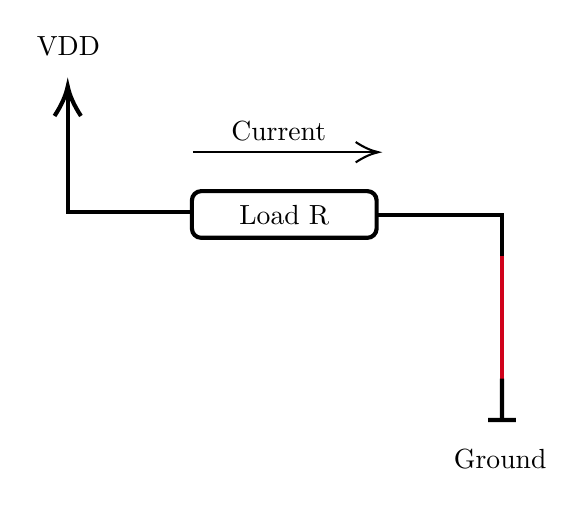
\begin{tikzpicture}[x=0.75pt,y=0.75pt,yscale=-1,xscale=1]
%uncomment if require: \path (0,240); %set diagram left start at 0, and has height of 240

%Straight Lines [id:da008984438739192413] 
\draw [color={rgb, 255:red, 0; green, 0; blue, 0 }  ,draw opacity=1 ][line width=1.5]    (91,99) -- (31.67,99) -- (31.67,41.33) ;
\draw [shift={(31.67,38.33)}, rotate = 450] [color={rgb, 255:red, 0; green, 0; blue, 0 }  ,draw opacity=1 ][line width=1.5]    (14.21,-6.37) .. controls (9.04,-2.99) and (4.3,-0.87) .. (0,0) .. controls (4.3,0.87) and (9.04,2.99) .. (14.21,6.37)   ;

%Rounded Rect [id:dp7662687261949606] 
\draw  [line width=1.5]  (91.5,93.25) .. controls (91.5,90.76) and (93.51,88.75) .. (96,88.75) -- (176,88.75) .. controls (178.49,88.75) and (180.5,90.76) .. (180.5,93.25) -- (180.5,106.75) .. controls (180.5,109.24) and (178.49,111.25) .. (176,111.25) -- (96,111.25) .. controls (93.51,111.25) and (91.5,109.24) .. (91.5,106.75) -- cycle ;
%Straight Lines [id:da19872085195301215] 
\draw [line width=1.5]    (181,100.25) -- (240.75,100.25) -- (240.75,120.13) ;


%Straight Lines [id:da8624965983535746] 
\draw [color={rgb, 255:red, 208; green, 2; blue, 27 }  ,draw opacity=1 ][line width=1.5]    (240.88,120.13) -- (240.88,179.13) ;


%Straight Lines [id:da9869704930235617] 
\draw [line width=1.5]    (240.88,179.13) -- (240.9,199) ;
\draw [shift={(240.9,199)}, rotate = 269.93] [color={rgb, 255:red, 0; green, 0; blue, 0 }  ][line width=1.5]    (0,6.71) -- (0,-6.71)   ;

%Straight Lines [id:da3727804380230437] 
\draw [line width=0.75]    (92,70) -- (179.33,70) ;
\draw [shift={(181.33,70)}, rotate = 180] [color={rgb, 255:red, 0; green, 0; blue, 0 }  ][line width=0.75]    (10.93,-4.9) .. controls (6.95,-2.3) and (3.31,-0.67) .. (0,0) .. controls (3.31,0.67) and (6.95,2.3) .. (10.93,4.9)   ;


% Text Node
\draw (136,100) node [scale=1] [align=left] {Load R};
% Text Node
\draw (133.33,59.67) node  [align=left] {Current};
% Text Node
\draw (240,218) node  [align=left] {Ground};
% Text Node
\draw (32,19) node  [align=left] {VDD};


\end{tikzpicture}
    \caption{short(low resistance) circuit between the load and the ground.} \label{fig:circuit1}
\end{figure}

If we connect an open circuit after the load (See Figure \ref{fig:circuit2}), it
will increase the resistance to a very high value, causing the current to become
zero effectively. If the current is zero then the voltage is also zero (Ohm's
Law).

\begin{figure}[!ht]
    \centering
    

\tikzset{every picture/.style={line width=0.75pt}} %set default line width to 0.75pt        

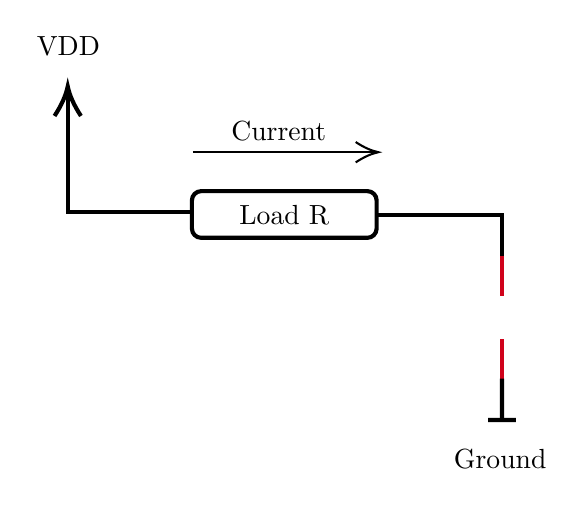
\begin{tikzpicture}[x=0.75pt,y=0.75pt,yscale=-1,xscale=1]
%uncomment if require: \path (0,240); %set diagram left start at 0, and has height of 240

%Straight Lines [id:da008984438739192413] 
\draw [color={rgb, 255:red, 0; green, 0; blue, 0 }  ,draw opacity=1 ][line width=1.5]    (91,99) -- (31.67,99) -- (31.67,41.33) ;
\draw [shift={(31.67,38.33)}, rotate = 450] [color={rgb, 255:red, 0; green, 0; blue, 0 }  ,draw opacity=1 ][line width=1.5]    (14.21,-6.37) .. controls (9.04,-2.99) and (4.3,-0.87) .. (0,0) .. controls (4.3,0.87) and (9.04,2.99) .. (14.21,6.37)   ;

%Rounded Rect [id:dp7662687261949606] 
\draw  [line width=1.5]  (91.5,93.25) .. controls (91.5,90.76) and (93.51,88.75) .. (96,88.75) -- (176,88.75) .. controls (178.49,88.75) and (180.5,90.76) .. (180.5,93.25) -- (180.5,106.75) .. controls (180.5,109.24) and (178.49,111.25) .. (176,111.25) -- (96,111.25) .. controls (93.51,111.25) and (91.5,109.24) .. (91.5,106.75) -- cycle ;
%Straight Lines [id:da19872085195301215] 
\draw [line width=1.5]    (181,100.25) -- (240.75,100.25) -- (240.75,120.13) ;


%Straight Lines [id:da8624965983535746] 
\draw [color={rgb, 255:red, 208; green, 2; blue, 27 }  ,draw opacity=1 ][line width=1.5]    (240.88,160) -- (240.88,179.13) ;


%Straight Lines [id:da9869704930235617] 
\draw [line width=1.5]    (240.88,179.13) -- (240.9,199) ;
\draw [shift={(240.9,199)}, rotate = 269.93] [color={rgb, 255:red, 0; green, 0; blue, 0 }  ][line width=1.5]    (0,6.71) -- (0,-6.71)   ;

%Straight Lines [id:da3727804380230437] 
\draw [line width=0.75]    (92,70) -- (179.33,70) ;
\draw [shift={(181.33,70)}, rotate = 180] [color={rgb, 255:red, 0; green, 0; blue, 0 }  ][line width=0.75]    (10.93,-4.9) .. controls (6.95,-2.3) and (3.31,-0.67) .. (0,0) .. controls (3.31,0.67) and (6.95,2.3) .. (10.93,4.9)   ;

%Straight Lines [id:da775249144810833] 
\draw [color={rgb, 255:red, 208; green, 2; blue, 27 }  ,draw opacity=1 ][line width=1.5]    (240.75,120.13) -- (240.75,139.25) ;



% Text Node
\draw (136,100) node [scale=1] [align=left] {Load R};
% Text Node
\draw (133.33,59.67) node  [align=left] {Current};
% Text Node
\draw (240,218) node  [align=left] {Ground};
% Text Node
\draw (32,19) node  [align=left] {VDD};


\end{tikzpicture}

    \caption{open circuit after the load.} \label{fig:circuit2}
\end{figure}

\subsubsection{Connecting in parallel}

If we connect an open circuit in parallel to the load (See Figure
\ref{fig:circuit3}), the current will flow only through the load path, so the
current on the open circuit will be 0. However, the voltage drop between both
points of the open circuit will be the same as the drop between the load sides.

\begin{figure}[!ht]
    \centering
    

\tikzset{every picture/.style={line width=0.75pt}} %set default line width to 0.75pt        

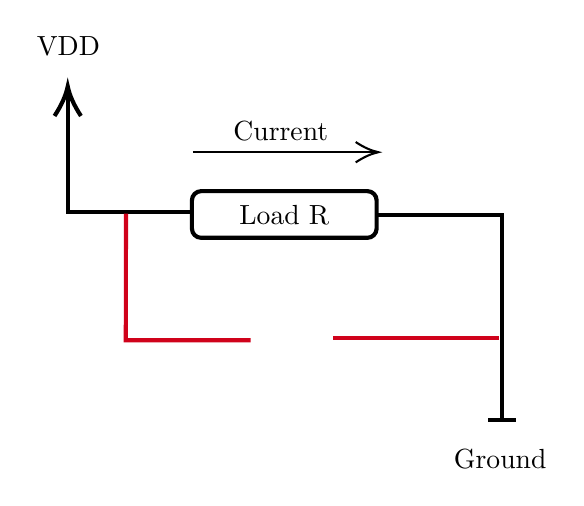
\begin{tikzpicture}[x=0.75pt,y=0.75pt,yscale=-1,xscale=1]
%uncomment if require: \path (0,250); %set diagram left start at 0, and has height of 250

%Straight Lines [id:da008984438739192413] 
\draw [color={rgb, 255:red, 0; green, 0; blue, 0 }  ,draw opacity=1 ][line width=1.5]    (91,99) -- (31.67,99) -- (31.67,41.33) ;
\draw [shift={(31.67,38.33)}, rotate = 450] [color={rgb, 255:red, 0; green, 0; blue, 0 }  ,draw opacity=1 ][line width=1.5]    (14.21,-6.37) .. controls (9.04,-2.99) and (4.3,-0.87) .. (0,0) .. controls (4.3,0.87) and (9.04,2.99) .. (14.21,6.37)   ;

%Rounded Rect [id:dp7662687261949606] 
\draw  [line width=1.5]  (91.5,93.25) .. controls (91.5,90.76) and (93.51,88.75) .. (96,88.75) -- (176,88.75) .. controls (178.49,88.75) and (180.5,90.76) .. (180.5,93.25) -- (180.5,106.75) .. controls (180.5,109.24) and (178.49,111.25) .. (176,111.25) -- (96,111.25) .. controls (93.51,111.25) and (91.5,109.24) .. (91.5,106.75) -- cycle ;
%Straight Lines [id:da19872085195301215] 
\draw [line width=1.5]    (181,100.25) -- (240.75,100.25) -- (240.75,199) ;
\draw [shift={(240.75,199)}, rotate = 270] [color={rgb, 255:red, 0; green, 0; blue, 0 }  ][line width=1.5]    (0,6.71) -- (0,-6.71)   ;

%Straight Lines [id:da3727804380230437] 
\draw [line width=0.75]    (92,70) -- (179.33,70) ;
\draw [shift={(181.33,70)}, rotate = 180] [color={rgb, 255:red, 0; green, 0; blue, 0 }  ][line width=0.75]    (10.93,-4.9) .. controls (6.95,-2.3) and (3.31,-0.67) .. (0,0) .. controls (3.31,0.67) and (6.95,2.3) .. (10.93,4.9)   ;

%Straight Lines [id:da4889722354710415] 
\draw [color={rgb, 255:red, 208; green, 2; blue, 27 }  ,draw opacity=1 ][line width=1.5]    (59.73,99.6) -- (59.65,160.6) -- (119.75,160.6) ;


%Straight Lines [id:da969741666977372] 
\draw [color={rgb, 255:red, 208; green, 2; blue, 27 }  ,draw opacity=1 ][line width=1.5]    (159.5,159.67) -- (239.25,159.67) ;



% Text Node
\draw (136,100) node [scale=1] [align=left] {Load R};
% Text Node
\draw (134.33,59.67) node  [align=left] {Current};
% Text Node
\draw (240,218) node  [align=left] {Ground};
% Text Node
\draw (32,19) node  [align=left] {VDD};


\end{tikzpicture}
    \caption{A close circuit in parallel to the load.} \label{fig:circuit3}
\end{figure}

If we connect a short circuit in parallel to the load (See Figure
\ref{fig:circuit4}), the current will ``prefer" flowing through it rather than
through the load, so the current through the load will be equal to zero, while
the current through the short circuit will be very high - by Ohm's law.

\begin{figure}[!ht]
    \centering
    

\tikzset{every picture/.style={line width=0.75pt}} %set default line width to 0.75pt        

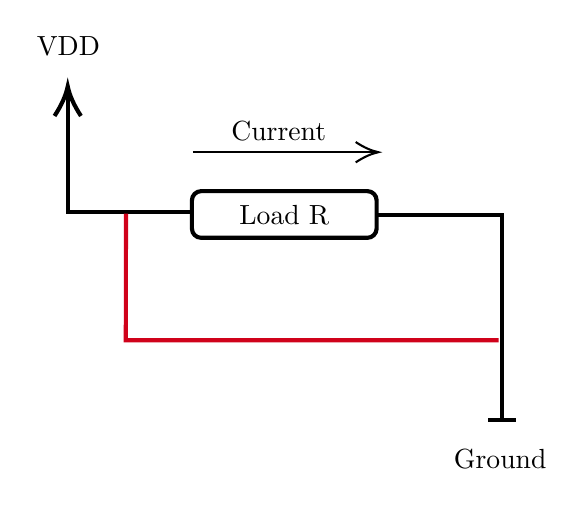
\begin{tikzpicture}[x=0.75pt,y=0.75pt,yscale=-1,xscale=1]
%uncomment if require: \path (0,230.3333282470703); %set diagram left start at 0, and has height of 230.3333282470703

%Straight Lines [id:da008984438739192413] 
\draw [color={rgb, 255:red, 0; green, 0; blue, 0 }  ,draw opacity=1 ][line width=1.5]    (91,99) -- (31.67,99) -- (31.67,41.33) ;
\draw [shift={(31.67,38.33)}, rotate = 450] [color={rgb, 255:red, 0; green, 0; blue, 0 }  ,draw opacity=1 ][line width=1.5]    (14.21,-6.37) .. controls (9.04,-2.99) and (4.3,-0.87) .. (0,0) .. controls (4.3,0.87) and (9.04,2.99) .. (14.21,6.37)   ;

%Rounded Rect [id:dp7662687261949606] 
\draw  [line width=1.5]  (91.5,93.25) .. controls (91.5,90.76) and (93.51,88.75) .. (96,88.75) -- (176,88.75) .. controls (178.49,88.75) and (180.5,90.76) .. (180.5,93.25) -- (180.5,106.75) .. controls (180.5,109.24) and (178.49,111.25) .. (176,111.25) -- (96,111.25) .. controls (93.51,111.25) and (91.5,109.24) .. (91.5,106.75) -- cycle ;
%Straight Lines [id:da19872085195301215] 
\draw [line width=1.5]    (181,100.25) -- (240.75,100.25) -- (240.75,199) ;
\draw [shift={(240.75,199)}, rotate = 270] [color={rgb, 255:red, 0; green, 0; blue, 0 }  ][line width=1.5]    (0,6.71) -- (0,-6.71)   ;

%Straight Lines [id:da3727804380230437] 
\draw [line width=0.75]    (92,70) -- (179.33,70) ;
\draw [shift={(181.33,70)}, rotate = 180] [color={rgb, 255:red, 0; green, 0; blue, 0 }  ][line width=0.75]    (10.93,-4.9) .. controls (6.95,-2.3) and (3.31,-0.67) .. (0,0) .. controls (3.31,0.67) and (6.95,2.3) .. (10.93,4.9)   ;

%Straight Lines [id:da4889722354710415] 
\draw [color={rgb, 255:red, 208; green, 2; blue, 27 }  ,draw opacity=1 ][line width=1.5]    (59.73,99.6) -- (59.65,160.6) -- (239.33,160.6) ;



% Text Node
\draw (136,100) node [scale=1] [align=left] {Load R};
% Text Node
\draw (133.33,59.67) node  [align=left] {Current};
% Text Node
\draw (240,218) node  [align=left] {Ground};
% Text Node
\draw (32,19) node  [align=left] {VDD};


\end{tikzpicture}
    \caption{A short circuit in parallel to the load.} \label{fig:circuit4}
\end{figure}

Since the cable is not a perfect conductor, some of the energy will be consumes
in the form of thermal work, so the cable will heat, and possibly melt and start
a fire.

\section{Measuring Power Consumption}

Next, as an attackers, we want to measure the power consumption of this load,
and to do so, we are going to use Ampermeter device.

\subsection{Ampermeter}

An Ampermeter (from \textbf{Am}pere \textbf{Meter}) is a device capable of
measuring the amount of electric current going through it. It has very low
resistance, so it doesn't interrupt the system connected to it.

\begin{figure}[!ht]
    \centering
    

\tikzset{every picture/.style={line width=0.75pt}} %set default line width to 0.75pt        

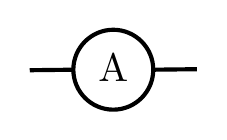
\begin{tikzpicture}[x=0.75pt,y=0.75pt,yscale=-1,xscale=1]
%uncomment if require: \path (0,80.33332824707031); %set diagram left start at 0, and has height of 80.33332824707031

%Shape: Circle [id:dp8443143357842926] 
\draw  [line width=1.5]  (42,40.58) .. controls (42,29.95) and (50.62,21.33) .. (61.25,21.33) .. controls (71.88,21.33) and (80.5,29.95) .. (80.5,40.58) .. controls (80.5,51.21) and (71.88,59.83) .. (61.25,59.83) .. controls (50.62,59.83) and (42,51.21) .. (42,40.58) -- cycle ;
%Straight Lines [id:da8989689187935987] 
\draw [line width=1.5]    (80.5,40.58) -- (101.5,40.33) ;


%Straight Lines [id:da08094666094700531] 
\draw [line width=1.5]    (21,40.83) -- (42,40.58) ;



% Text Node
\draw (61.25,39.58) node [scale=1.44] [align=left] {A};


\end{tikzpicture}
    \caption{Ampermeter Symbol in Circuit Diagrams.} \label{fig:ampermeter}
\end{figure}

\subsubsection{Using Ampermeter to measure power consumption}

We need to ``cut" the wire connected to the load and connect both sides to the
Ampermeter.(See \Cref{fig:circuit5})

Doing so will cause all current flowing through the load to pass through the
Ampermeter as well, so we will be able to read the current at any given time.
The resistance of the Ampermeter is very low so it will not affect the voltage
that going through the load that will have the same voltage drop as before. 

\begin{figure}[!ht]
    \centering
    

\tikzset{every picture/.style={line width=0.75pt}} %set default line width to 0.75pt        

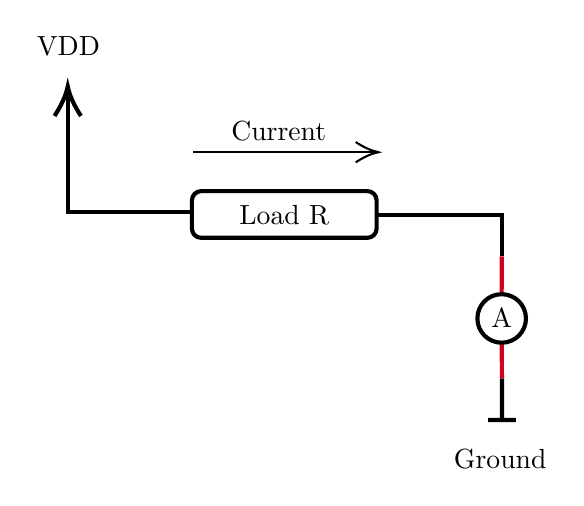
\begin{tikzpicture}[x=0.75pt,y=0.75pt,yscale=-1,xscale=1]
%uncomment if require: \path (0,240); %set diagram left start at 0, and has height of 240

%Straight Lines [id:da008984438739192413] 
\draw [color={rgb, 255:red, 0; green, 0; blue, 0 }  ,draw opacity=1 ][line width=1.5]    (91,99) -- (31.67,99) -- (31.67,41.33) ;
\draw [shift={(31.67,38.33)}, rotate = 450] [color={rgb, 255:red, 0; green, 0; blue, 0 }  ,draw opacity=1 ][line width=1.5]    (14.21,-6.37) .. controls (9.04,-2.99) and (4.3,-0.87) .. (0,0) .. controls (4.3,0.87) and (9.04,2.99) .. (14.21,6.37)   ;

%Rounded Rect [id:dp7662687261949606] 
\draw  [line width=1.5]  (91.5,93.25) .. controls (91.5,90.76) and (93.51,88.75) .. (96,88.75) -- (176,88.75) .. controls (178.49,88.75) and (180.5,90.76) .. (180.5,93.25) -- (180.5,106.75) .. controls (180.5,109.24) and (178.49,111.25) .. (176,111.25) -- (96,111.25) .. controls (93.51,111.25) and (91.5,109.24) .. (91.5,106.75) -- cycle ;
%Straight Lines [id:da19872085195301215] 
\draw [line width=1.5]    (181,100.25) -- (240.75,100.25) -- (240.75,120.13) ;


%Straight Lines [id:da8624965983535746] 
\draw [color={rgb, 255:red, 208; green, 2; blue, 27 }  ,draw opacity=1 ][line width=1.5]    (240.74,161.79) -- (240.88,179.13) ;


%Straight Lines [id:da9869704930235617] 
\draw [line width=1.5]    (240.88,179.13) -- (240.9,199) ;
\draw [shift={(240.9,199)}, rotate = 269.93] [color={rgb, 255:red, 0; green, 0; blue, 0 }  ][line width=1.5]    (0,6.71) -- (0,-6.71)   ;

%Straight Lines [id:da3727804380230437] 
\draw [line width=0.75]    (92,70) -- (179.33,70) ;
\draw [shift={(181.33,70)}, rotate = 180] [color={rgb, 255:red, 0; green, 0; blue, 0 }  ][line width=0.75]    (10.93,-4.9) .. controls (6.95,-2.3) and (3.31,-0.67) .. (0,0) .. controls (3.31,0.67) and (6.95,2.3) .. (10.93,4.9)   ;

%Straight Lines [id:da775249144810833] 
\draw [color={rgb, 255:red, 208; green, 2; blue, 27 }  ,draw opacity=1 ][line width=1.5]    (240.75,120.13) -- (240.74,138.4) ;


%Shape: Circle [id:dp5127141465445768] 
\draw  [line width=1.5]  (229.04,150.09) .. controls (229.04,143.63) and (234.28,138.4) .. (240.74,138.4) .. controls (247.2,138.4) and (252.44,143.63) .. (252.44,150.09) .. controls (252.44,156.55) and (247.2,161.79) .. (240.74,161.79) .. controls (234.28,161.79) and (229.04,156.55) .. (229.04,150.09) -- cycle ;

% Text Node
\draw (136,100) node [scale=1] [align=left] {Load R};
% Text Node
\draw (133.33,59.67) node  [align=left] {Current};
% Text Node
\draw (240,218) node  [align=left] {Ground};
% Text Node
\draw (32,19) node  [align=left] {VDD};
% Text Node
\draw (240.74,150.09) node  [align=left] {A};


\end{tikzpicture}
    \caption{an Ampermeter connected in serial.} \label{fig:circuit5}
\end{figure}

Now we will measure the current going through the ampermeter and next we will
convert the current in order to find the power consumption of the load.

In case we know the voltage (i.e. a 5V battery, a 220V power socket), we can
compute the power consumption: $P=I*V$.

The problem: sometimes, we don't want (or simply can't) cut the circuit after
the load in order to connect an Ampermeter, and this is a way that the architect
of the device are trying to protect it. So, let's see if we can use the
ampermeter without cutting anything, and let's connect it in parallel to the
load. (See \Cref{fig:circuit6})

\begin{figure}[!ht]
    \centering
    

\tikzset{every picture/.style={line width=0.75pt}} %set default line width to 0.75pt        

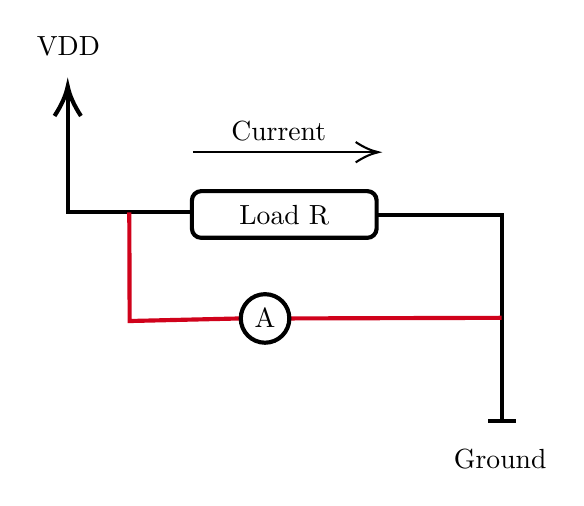
\begin{tikzpicture}[x=0.75pt,y=0.75pt,yscale=-1,xscale=1]
%uncomment if require: \path (0,240); %set diagram left start at 0, and has height of 240

%Straight Lines [id:da008984438739192413] 
\draw [color={rgb, 255:red, 0; green, 0; blue, 0 }  ,draw opacity=1 ][line width=1.5]    (91,99) -- (31.67,99) -- (31.67,41.33) ;
\draw [shift={(31.67,38.33)}, rotate = 450] [color={rgb, 255:red, 0; green, 0; blue, 0 }  ,draw opacity=1 ][line width=1.5]    (14.21,-6.37) .. controls (9.04,-2.99) and (4.3,-0.87) .. (0,0) .. controls (4.3,0.87) and (9.04,2.99) .. (14.21,6.37)   ;

%Rounded Rect [id:dp7662687261949606] 
\draw  [line width=1.5]  (91.5,93.25) .. controls (91.5,90.76) and (93.51,88.75) .. (96,88.75) -- (176,88.75) .. controls (178.49,88.75) and (180.5,90.76) .. (180.5,93.25) -- (180.5,106.75) .. controls (180.5,109.24) and (178.49,111.25) .. (176,111.25) -- (96,111.25) .. controls (93.51,111.25) and (91.5,109.24) .. (91.5,106.75) -- cycle ;
%Straight Lines [id:da19872085195301215] 
\draw [line width=1.5]    (181,100.25) -- (240.75,100.25) -- (240.75,199.33) ;
\draw [shift={(240.75,199.33)}, rotate = 270] [color={rgb, 255:red, 0; green, 0; blue, 0 }  ][line width=1.5]    (0,6.71) -- (0,-6.71)   ;

%Straight Lines [id:da8624965983535746] 
\draw [color={rgb, 255:red, 208; green, 2; blue, 27 }  ,draw opacity=1 ][line width=1.5]    (138.44,150.09) -- (240.75,149.79) ;


%Straight Lines [id:da3727804380230437] 
\draw [line width=0.75]    (92,70) -- (179.33,70) ;
\draw [shift={(181.33,70)}, rotate = 180] [color={rgb, 255:red, 0; green, 0; blue, 0 }  ][line width=0.75]    (10.93,-4.9) .. controls (6.95,-2.3) and (3.31,-0.67) .. (0,0) .. controls (3.31,0.67) and (6.95,2.3) .. (10.93,4.9)   ;

%Straight Lines [id:da775249144810833] 
\draw [color={rgb, 255:red, 208; green, 2; blue, 27 }  ,draw opacity=1 ][line width=1.5]    (61.33,99) -- (61.5,151.33) -- (115.04,150.09) ;


%Shape: Circle [id:dp5127141465445768] 
\draw  [line width=1.5]  (115.04,150.09) .. controls (115.04,143.63) and (120.28,138.4) .. (126.74,138.4) .. controls (133.2,138.4) and (138.44,143.63) .. (138.44,150.09) .. controls (138.44,156.55) and (133.2,161.79) .. (126.74,161.79) .. controls (120.28,161.79) and (115.04,156.55) .. (115.04,150.09) -- cycle ;

% Text Node
\draw (136,100) node [scale=1] [align=left] {Load R};
% Text Node
\draw (133.33,59.67) node  [align=left] {Current};
% Text Node
\draw (240,218) node  [align=left] {Ground};
% Text Node
\draw (32,19) node  [align=left] {VDD};
% Text Node
\draw (126.74,150.09) node  [align=left] {A};


\end{tikzpicture}
    \caption{An ampermeter connected in parallel to the load} \label{fig:circuit6}
\end{figure}

Connecting the ampermeter this way will burn the ampermeter as it has no
resistance and so, all of the current will flow through it. So, instead of
ampermeter we can use a voltmeter as follows (See \Cref{fig:circuit7}):

\subsection{Voltmeter}

\begin{figure}[!ht]
    \centering
    

\tikzset{every picture/.style={line width=0.75pt}} %set default line width to 0.75pt        

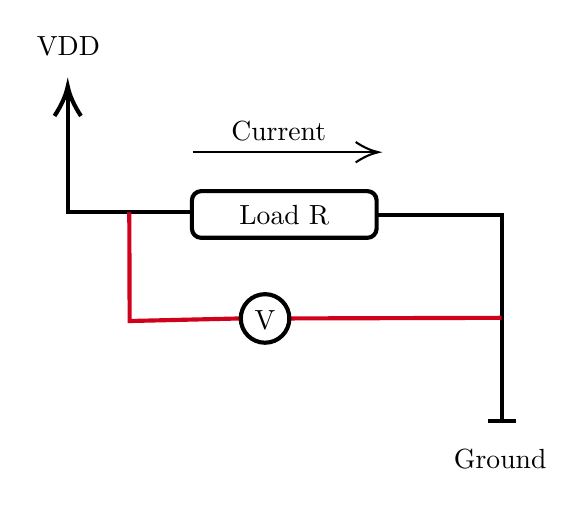
\begin{tikzpicture}[x=0.75pt,y=0.75pt,yscale=-1,xscale=1]
%uncomment if require: \path (0,240); %set diagram left start at 0, and has height of 240

%Straight Lines [id:da008984438739192413] 
\draw [color={rgb, 255:red, 0; green, 0; blue, 0 }  ,draw opacity=1 ][line width=1.5]    (91,99) -- (31.67,99) -- (31.67,41.33) ;
\draw [shift={(31.67,38.33)}, rotate = 450] [color={rgb, 255:red, 0; green, 0; blue, 0 }  ,draw opacity=1 ][line width=1.5]    (14.21,-6.37) .. controls (9.04,-2.99) and (4.3,-0.87) .. (0,0) .. controls (4.3,0.87) and (9.04,2.99) .. (14.21,6.37)   ;

%Rounded Rect [id:dp7662687261949606] 
\draw  [line width=1.5]  (91.5,93.25) .. controls (91.5,90.76) and (93.51,88.75) .. (96,88.75) -- (176,88.75) .. controls (178.49,88.75) and (180.5,90.76) .. (180.5,93.25) -- (180.5,106.75) .. controls (180.5,109.24) and (178.49,111.25) .. (176,111.25) -- (96,111.25) .. controls (93.51,111.25) and (91.5,109.24) .. (91.5,106.75) -- cycle ;
%Straight Lines [id:da19872085195301215] 
\draw [line width=1.5]    (181,100.25) -- (240.75,100.25) -- (240.75,199.33) ;
\draw [shift={(240.75,199.33)}, rotate = 270] [color={rgb, 255:red, 0; green, 0; blue, 0 }  ][line width=1.5]    (0,6.71) -- (0,-6.71)   ;

%Straight Lines [id:da8624965983535746] 
\draw [color={rgb, 255:red, 208; green, 2; blue, 27 }  ,draw opacity=1 ][line width=1.5]    (138.44,150.09) -- (240.75,149.79) ;


%Straight Lines [id:da3727804380230437] 
\draw [line width=0.75]    (92,70) -- (179.33,70) ;
\draw [shift={(181.33,70)}, rotate = 180] [color={rgb, 255:red, 0; green, 0; blue, 0 }  ][line width=0.75]    (10.93,-4.9) .. controls (6.95,-2.3) and (3.31,-0.67) .. (0,0) .. controls (3.31,0.67) and (6.95,2.3) .. (10.93,4.9)   ;

%Straight Lines [id:da775249144810833] 
\draw [color={rgb, 255:red, 208; green, 2; blue, 27 }  ,draw opacity=1 ][line width=1.5]    (61.33,99) -- (61.5,151.33) -- (115.04,150.09) ;


%Shape: Circle [id:dp5127141465445768] 
\draw  [line width=1.5]  (115.04,150.09) .. controls (115.04,143.63) and (120.28,138.4) .. (126.74,138.4) .. controls (133.2,138.4) and (138.44,143.63) .. (138.44,150.09) .. controls (138.44,156.55) and (133.2,161.79) .. (126.74,161.79) .. controls (120.28,161.79) and (115.04,156.55) .. (115.04,150.09) -- cycle ;

% Text Node
\draw (136,100) node [scale=1] [align=left] {Load R};
% Text Node
\draw (133.33,59.67) node  [align=left] {Current};
% Text Node
\draw (240,218) node  [align=left] {Ground};
% Text Node
\draw (32,19) node  [align=left] {VDD};
% Text Node
\draw (126.74,151.09) node  [align=left] {V};


\end{tikzpicture}
    \caption{a voltmeter connected in parallel to the load} \label{fig:circuit7}
\end{figure}

The voltmeter resistance is very very high so the current will not go through
it. The voltmeter is measuring the voltage drop between one side of the load and
the other side of it. If we want to measure the current using the voltmeter we
are taking a load with a very small resistance and connect it as follows (See
\Cref{fig:circuit8}):

\begin{figure}[!ht]
    \centering
    

\tikzset{every picture/.style={line width=0.75pt}} %set default line width to 0.75pt        

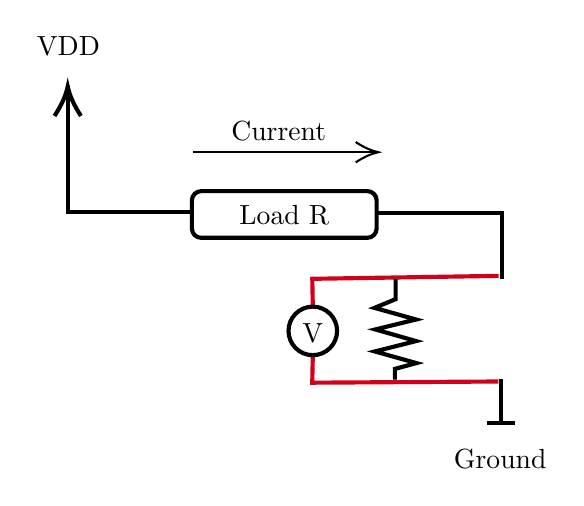
\begin{tikzpicture}[x=0.75pt,y=0.75pt,yscale=-1,xscale=1]
%uncomment if require: \path (0,230.3333282470703); %set diagram left start at 0, and has height of 230.3333282470703

%Straight Lines [id:da008984438739192413] 
\draw [color={rgb, 255:red, 0; green, 0; blue, 0 }  ,draw opacity=1 ][line width=1.5]    (91,99) -- (31.67,99) -- (31.67,41.33) ;
\draw [shift={(31.67,38.33)}, rotate = 450] [color={rgb, 255:red, 0; green, 0; blue, 0 }  ,draw opacity=1 ][line width=1.5]    (14.21,-6.37) .. controls (9.04,-2.99) and (4.3,-0.87) .. (0,0) .. controls (4.3,0.87) and (9.04,2.99) .. (14.21,6.37)   ;

%Rounded Rect [id:dp7662687261949606] 
\draw  [line width=1.5]  (91.5,93.25) .. controls (91.5,90.76) and (93.51,88.75) .. (96,88.75) -- (176,88.75) .. controls (178.49,88.75) and (180.5,90.76) .. (180.5,93.25) -- (180.5,106.75) .. controls (180.5,109.24) and (178.49,111.25) .. (176,111.25) -- (96,111.25) .. controls (93.51,111.25) and (91.5,109.24) .. (91.5,106.75) -- cycle ;
%Straight Lines [id:da19872085195301215] 
\draw [line width=1.5]    (181,99.25) -- (240.75,99.25) -- (240.75,131.08) ;


%Straight Lines [id:da8624965983535746] 
\draw [color={rgb, 255:red, 208; green, 2; blue, 27 }  ,draw opacity=1 ][line width=1.5]    (149.74,144.4) -- (149.5,131) -- (239.25,129.58) ;


%Straight Lines [id:da3727804380230437] 
\draw [line width=0.75]    (92,70) -- (179.33,70) ;
\draw [shift={(181.33,70)}, rotate = 180] [color={rgb, 255:red, 0; green, 0; blue, 0 }  ][line width=0.75]    (10.93,-4.9) .. controls (6.95,-2.3) and (3.31,-0.67) .. (0,0) .. controls (3.31,0.67) and (6.95,2.3) .. (10.93,4.9)   ;

%Straight Lines [id:da775249144810833] 
\draw [color={rgb, 255:red, 208; green, 2; blue, 27 }  ,draw opacity=1 ][line width=1.5]    (149.74,167.79) -- (149.48,181.05) -- (239.19,180.47) ;


%Shape: Circle [id:dp5127141465445768] 
\draw  [line width=1.5]  (138.04,156.09) .. controls (138.04,149.63) and (143.28,144.4) .. (149.74,144.4) .. controls (156.2,144.4) and (161.44,149.63) .. (161.44,156.09) .. controls (161.44,162.55) and (156.2,167.79) .. (149.74,167.79) .. controls (143.28,167.79) and (138.04,162.55) .. (138.04,156.09) -- cycle ;
%Straight Lines [id:da5151277448838241] 
\draw [line width=1.5]    (240.32,179.37) -- (240.32,200.37) ;
\draw [shift={(240.32,200.37)}, rotate = 270] [color={rgb, 255:red, 0; green, 0; blue, 0 }  ][line width=1.5]    (0,6.71) -- (0,-6.71)   ;

%Straight Lines [id:da45585704731206445] 
\draw [line width=1.5]    (189.67,131.2) -- (189.67,140.8) -- (179.47,145) -- (199.47,150.6) -- (179.87,155.4) -- (199.47,161) -- (179.67,166) -- (199.67,171.6) -- (189.27,174.4) -- (189.27,179.6) ;



% Text Node
\draw (136,100) node [scale=1] [align=left] {Load R};
% Text Node
\draw (133.33,59.67) node  [align=left] {Current};
% Text Node
\draw (240,218) node  [align=left] {Ground};
% Text Node
\draw (32,19) node  [align=left] {VDD};
% Text Node
\draw (149.74,157.09) node  [align=left] {V};


\end{tikzpicture}
    \caption{Circuit 8.} \label{fig:circuit8}
\end{figure}

This way, because of the current divider, by connecting a Voltmeter in parallel
with a very small and accurate resistor, we can measure the electric current
using Ohm's law: $I=V/R$
 
Summary: we learned what is Power Consumption and how we can measure it. A very
important fact is that \textbf{Power Consumption varies with time!}. If we can
find a relationship between the secret information we want to extract and the
power consumption, we can recover this information by measuring the power
consumption over time.

\subsection{Types of electronic components}

In general there are two types of elements in the circuit, the first one are
Passive devices like a resistors (a passive two-terminal electrical component
that implements electrical resistance as a circuit element), inductors (is a
passive two-terminal electrical component that stores energy in a magnetic field
when electric current flows through it), capacitors and diodes. And there are
Active devices like transistors (a semiconductor device used to amplify or
switch electronic signals and electrical power), amplifiers (an electronic
device that can increase the power of a signal (a time-varying voltage or
current)) and ICs. From our perspective, the Active devices are much more
interesting for us (attackers) as they are using electricity in order to control
electricity. One example can be an amplifier that has audio signal and power
supply as inputs and it generates a greater audio signal as an output using the
power supply. 

\begin{figure}[!ht]
	\centering
	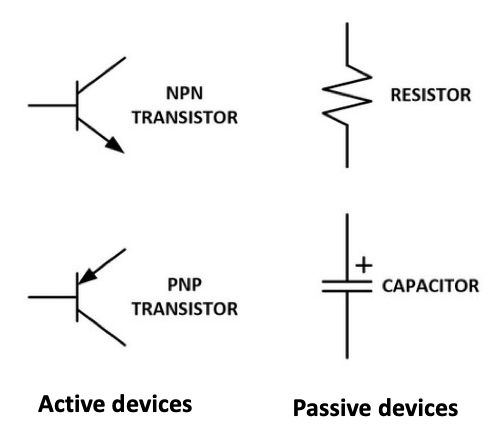
\includegraphics{images/type_of_electronic_components.png}
	\caption{Examples of electronic components.} \label{fig:type_of_electronic_components}
\end{figure}

Another interesting active element for this course is a transistor. In an
integrated circuits, there are a lot of active devices such as transistors  that
if we can analyze their behavior we can learn about the data that they are
processing. So when we look at the final consumption of these active elements,
we can figure out some kind of secrets.

There are many kind of transistors and we will concentrate on understanding a
certain type called Field-Effect Transistor.

\begin{figure}[!ht]
	\centering
	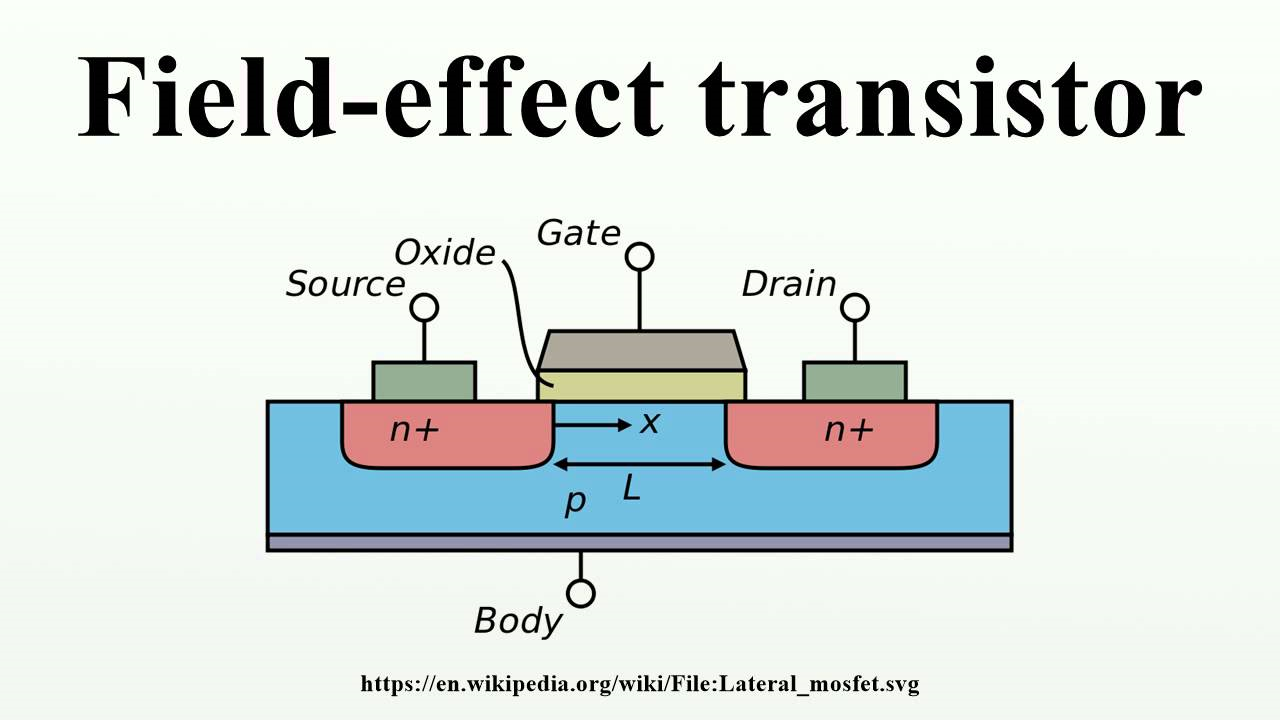
\includegraphics{images/field_effect_transistor.png}
	\caption{Field-Effect Transistor.} \label{fig:field_effect_transistor}
\end{figure}

\subsection{Field-Effect Transistor}

The field-effect transistor (FET) is an electronic device which uses an electric
field to control the flow of current. FETs are 3-terminalled devices, having a
source, gate, and drain terminal. FETs control the flow of current by the
application of a voltage to the gate terminal, which in turn alters the
conductivity between the drain and source terminals. In order to understand FET
first we need to dive into the basics of semiconductors.

\subsection{Semiconductors}

A semiconductor is a substance, usually a solid chemical element or compound,
that can conduct electricity under some conditions but not others, making it a
good medium for the control of electrical current. Its conductance varies
depending on the current or voltage applied to a control electrode, or on the
intensity of irradiation by infrared (IR), visible light, ultraviolet (UV), or X
rays. In general, transistors are made of semiconducting materials such as
silicon. There are a conductor like copper or gold and there are insulators like
plastic or glass.

Silicon atom has three parts: neutrons (not relevant for our use), protons with
the positive charge (heavy) and electrons that have the negative charge and they
are small and dynamic. Silicon atom has four electrons in its outer orbital and
when we have a crystal silicon those 4 electrons are set in place very nicely.
It means that pure silicon is a very bad conductor as  conducting means that the
electrons can move around and in this case they are very comfortable where they
are.

Metals can be good conductors of electricity as they have ``free electrons" that
can move easily from atom to atom, the electricity involves the flow of
electrons. As all of the outer electrons in Silicon crystal are involved in
perfect covalent bonds, they cannot move around. So, silicon crystal is nearly
insulator and very little electricity will flow through it. We can change the
behavior of  the silicon and turn it into a conductor by doping it. In doping,
we mix a small amount of an impurity into the silicon crystal.

There are two types of impurities:
\begin{itemize}
    \item N-type – where phosphorus or arsenic is added to the silicon in small
    quantities. They both have  five outer electrons, so one of them is out of
    place when they get into the silicon lattice. While having nothing to bond
    to, the fifth electron is free to move around. As electrons have a negative
    charge, this kind of impurity called N-type.
    \item P-type - where boron or gallium is added to the silicon. They both
    have only three outer electrons. So, when we mixed them into the silicon
    lattice, there will be ``holes" in the lattice where a silicon electron has
    nothing to bond to. The hole is looking for an electron from a neighbor atom
    and when that's happens the hole is ``moving". As the absence of an electron
    creates the effect of a positive charge, this kind of impurity called
    P-type.
\end{itemize}

\subsection{ How does Field-Effect Transistor work? }

In the Field-Effect Transistor there are (as shown in
\Cref{fig:field_effect_transistor}) n+ areas (N-type) and P area (P-type). The
n+ area contains a lot of free electrons and the P area contains a lot of
'holes'. When no electricity is connected to the gate, the free electrons from
the N+ are moving to the holes so there are no free electrons within the
semiconductor itself. That means electrons can't move from the source to the
drain i.e. open circuit. When electricity is connected to the gate it charge a
lot of free electrons to it. The free electrons in the gate can't move to the
silicon itself as there is an oxide layer between them, but is pushes the
electrons in the silicon down to the body in a way there are holes between the
source and the drain. That way electrons can move from the source to the drain
freely and we have close circuit. 

\begin{figure}[!ht]
    \centering
    

\tikzset{every picture/.style={line width=0.75pt}} %set default line width to 0.75pt        

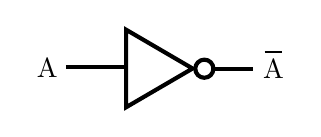
\begin{tikzpicture}[x=0.75pt,y=0.75pt,yscale=-1,xscale=1]
%uncomment if require: \path (0,219); %set diagram left start at 0, and has height of 219

%Straight Lines [id:da07885295239893186] 
\draw [line width=1.5]    (40,39.33) -- (68.5,39.33) ;


%Straight Lines [id:da2596764371394711] 
\draw [line width=1.5]    (110.02,40.17) -- (130.25,40.17) ;

\draw [shift={(106.67,40.17)}, rotate = 0] [color={rgb, 255:red, 0; green, 0; blue, 0 }  ][line width=1.5]      (0, 0) circle [x radius= 4.36, y radius= 4.36]   ;
%Straight Lines [id:da4451475450468101] 
\draw [line width=0.75]    (135.67,32.17) -- (144,32.17) ;


%Flowchart: Extract [id:dp4235554887602122] 
\draw  [line width=1.5]  (101,40.07) -- (69,58.73) -- (69,21.4) -- cycle ;

% Text Node
\draw (31,40) node  [align=left] {A};
% Text Node
\draw (140,40.5) node  [align=left] {A};


\end{tikzpicture}
    \caption{NOT Gate.} \label{fig:not}
\end{figure}

\subsection{ NOT Gate CMOS}

\begin{figure}[!ht]
    \centering
    

\tikzset{every picture/.style={line width=0.75pt}} %set default line width to 0.75pt        

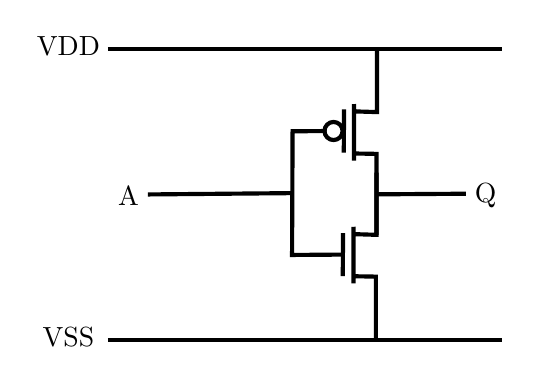
\begin{tikzpicture}[x=0.75pt,y=0.75pt,yscale=-1,xscale=1]
%uncomment if require: \path (0,201.3333282470703); %set diagram left start at 0, and has height of 201.3333282470703

%Straight Lines [id:da07885295239893186] 
\draw [line width=1.5]    (51,30.33) -- (240.75,30.33) ;


%Straight Lines [id:da39856222237487815] 
\draw [line width=1.5]    (180.67,30.67) -- (180.67,60.67) -- (169.71,60.33) -- (169.6,56.8) -- (169.6,84.05) -- (169.6,80.62) -- (180.4,80.8) -- (180.4,119.81) ;


%Straight Lines [id:da5857134524935192] 
\draw [line width=1.5]    (180.4,89.81) -- (180.4,119.81) -- (169.45,119.47) -- (169.33,115.94) -- (169.33,143.19) -- (169.33,139.76) -- (180.13,139.94) -- (180.13,170) ;


%Straight Lines [id:da21313521807196745] 
\draw [line width=1.5]    (51,170.33) -- (240.75,170.33) ;


%Straight Lines [id:da5667092258145612] 
\draw [line width=1.5]    (180.4,100.3) -- (223.5,100) ;


%Straight Lines [id:da6991442899200719] 
\draw [line width=1.5]    (164.67,80.16) -- (164.8,59.4) ;


%Straight Lines [id:da08031166754703278] 
\draw [line width=1.5]    (164.25,129.33) -- (139.75,129.5) -- (140,69.92) -- (156.38,69.8) ;
\draw [shift={(159.73,69.78)}, rotate = 359.6] [color={rgb, 255:red, 0; green, 0; blue, 0 }  ][line width=1.5]      (0, 0) circle [x radius= 4.36, y radius= 4.36]   ;

%Straight Lines [id:da21308267181792218] 
\draw [line width=1.5]    (164.18,139.71) -- (164.32,118.96) ;


%Straight Lines [id:da40299410186396645] 
\draw [line width=1.5]    (70.25,100.35) -- (139.88,99.71) ;



% Text Node
\draw (32,29) node  [align=left] {VDD};
% Text Node
\draw (32,169) node  [align=left] {VSS};
% Text Node
\draw (233,101) node  [align=left] {Q};
% Text Node
\draw (61,101) node  [align=left] {A};


\end{tikzpicture}
    \caption{Circuit 9.} \label{fig:circuit9}
\end{figure}

How does CMOS work? When the voltage of input A is low A = 0, the upper
transistor's channel is closed and we have a connection between Vdd(1) and Q, so
Q = 1, this is a Pull Up Network. And when the voltage of input A is high, then
the lower transistor's channel is closed and we have a connection between Vss(0)
and Q, so Q = 0, this is a Pull Down Network. A question is raised – when does
this circuit consume power? There is almost no power consume as there is no
connection between Vdd and Vss at any time. Although when CMOS is switching
between states, there is a minor power usage and we will see how we can use it
for our purpose.

Following is the NOT table:

\begin{table}
    \centering
    \caption{NOT gate truth table.}
    \begin{tabular}{llll}
        \toprule
        \textbf{input}  & A     & 0 & 1 \\ \midrule \textbf{output} & Not A & 1
        & 0 \\ \bottomrule
    \end{tabular}
\end{table} 

\subsection{ AND Gate CMOS}

Next we will see how to build a bit more complicated gate using 4 transistors.
Following is the AND gate diagram:

\begin{figure}[!ht]
    \centering
    

\tikzset{every picture/.style={line width=0.75pt}} %set default line width to 0.75pt        

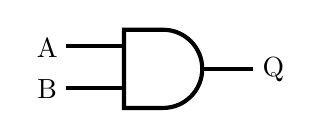
\begin{tikzpicture}[x=0.75pt,y=0.75pt,yscale=-1,xscale=1]
%uncomment if require: \path (0,80.33332824707031); %set diagram left start at 0, and has height of 80.33332824707031

%Straight Lines [id:da07885295239893186] 
\draw [line width=1.5]    (40,29.33) -- (68.5,29.33) ;


%Flowchart: Delay [id:dp4724078764954891] 
\draw  [line width=1.5]  (68,21.33) -- (86.83,21.33) .. controls (97.23,21.33) and (105.67,29.77) .. (105.67,40.17) .. controls (105.67,50.57) and (97.23,59) .. (86.83,59) -- (68,59) -- cycle ;
%Straight Lines [id:da5877789079181] 
\draw [line width=1.5]    (40,49.33) -- (68.5,49.33) ;


%Straight Lines [id:da2596764371394711] 
\draw [line width=1.5]    (106.67,40.17) -- (130.25,40.17) ;



% Text Node
\draw (31,30) node  [align=left] {A};
% Text Node
\draw (31,50) node  [align=left] {B};
% Text Node
\draw (140,40.5) node  [align=left] {Q};


\end{tikzpicture}
    \caption{AND Gate.} \label{fig:and}
\end{figure}

We will implement the gate using 4 transistors to support the following AND
table:

\begin{table}[!ht]
    \centering
    \caption{AND gate truth table.}
    \begin{tabular}{lllll}
        \toprule
        \textbf{input a} & 0 & 0 & 1 & 1 \\ \midrule \textbf{input b} & 0 & 1 &
        0 & 1 \\ \midrule \textbf{output}  & 0 & 0 & 0 & 1 \\ \bottomrule
    \end{tabular}
\end{table}

First we want to build the Pull Up Network, so for input A and B, for A=B=1 then
the output Q is 1. Then we will build the Pull Down Network to support the other
combination from the table to deliver 0 as the output Q. Sometimes we don't want
to have combination using the circuits, but we want to store information in it,
next we will talk about another type of circuits called storage circuit or
Sequential Circuit.

\subsection{ Storage/Sequential Circuit }

A latch or flip-flop is a circuit that has two stable states and can be used to
store state information. 
\begin{figure}[!ht]
    \centering
    

\tikzset{every picture/.style={line width=0.75pt}} %set default line width to 0.75pt        

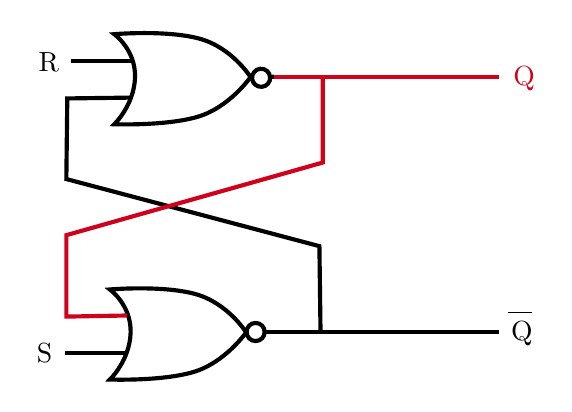
\begin{tikzpicture}[x=0.75pt,y=0.75pt,yscale=-1,xscale=1]
%uncomment if require: \path (0,210.66666412353516); %set diagram left start at 0, and has height of 210.66666412353516

%Shape: Polygon Curved [id:ds6291230594537647] 
\draw  [color={rgb, 255:red, 0; green, 0; blue, 0 }  ,draw opacity=1 ][line width=1.5]  (64.57,15.54) .. controls (64.57,15.54) and (75.02,23.03) .. (74.57,36.44) .. controls (74.11,49.84) and (64.57,58.93) .. (64.57,58.93) .. controls (64.57,58.93) and (89.67,59.83) .. (104.89,55.29) .. controls (120.12,50.74) and (130.23,36.21) .. (130.23,36.21) .. controls (130.23,36.21) and (121.33,21.89) .. (105.43,17.64) .. controls (89.52,13.4) and (64.57,15.54) .. (64.57,15.54) -- cycle ;
%Straight Lines [id:da32731251553352636] 
\draw [color={rgb, 255:red, 0; green, 0; blue, 0 }  ,draw opacity=1 ][line width=1.5]    (43.93,28.6) -- (72.96,28.6) ;


%Straight Lines [id:da3869103872130202] 
\draw [color={rgb, 255:red, 0; green, 0; blue, 0 }  ,draw opacity=1 ][line width=1.5]    (163.94,158.49) -- (163.41,117.67) -- (41.48,85.33) -- (41.94,46.49) -- (72.16,46.1) ;


%Straight Lines [id:da1720618143634285] 
\draw [color={rgb, 255:red, 0; green, 0; blue, 0 }  ,draw opacity=1 ][line width=1.5]    (138.66,36.27) -- (141.5,36.02) ;

\draw [shift={(135.32,36.55)}, rotate = 355.1] [color={rgb, 255:red, 0; green, 0; blue, 0 }  ,draw opacity=1 ][line width=1.5]      (0, 0) circle [x radius= 4.36, y radius= 4.36]   ;
%Straight Lines [id:da9259051839045029] 
\draw [color={rgb, 255:red, 0; green, 0; blue, 0 }  ,draw opacity=1 ][line width=1.5]    (136.02,159.02) -- (250,159.02) ;

\draw [shift={(132.67,159.02)}, rotate = 0] [color={rgb, 255:red, 0; green, 0; blue, 0 }  ,draw opacity=1 ][line width=1.5]      (0, 0) circle [x radius= 4.36, y radius= 4.36]   ;
%Shape: Polygon Curved [id:ds45090218745840094] 
\draw  [color={rgb, 255:red, 0; green, 0; blue, 0 }  ,draw opacity=1 ][line width=1.5]  (62.45,138.53) .. controls (62.45,138.53) and (72.9,146.03) .. (72.45,159.43) .. controls (71.99,172.84) and (62.45,181.93) .. (62.45,181.93) .. controls (62.45,181.93) and (87.55,182.82) .. (102.77,178.28) .. controls (118,173.74) and (128.11,159.21) .. (128.11,159.21) .. controls (128.11,159.21) and (119.21,144.88) .. (103.3,140.64) .. controls (87.4,136.4) and (62.45,138.53) .. (62.45,138.53) -- cycle ;
%Straight Lines [id:da4647074828700599] 
\draw [color={rgb, 255:red, 0; green, 0; blue, 0 }  ,draw opacity=1 ][line width=1.5]    (40.75,169.09) -- (69.78,169.09) ;


%Straight Lines [id:da5333172740033338] 
\draw [color={rgb, 255:red, 208; green, 2; blue, 27 }  ,draw opacity=1 ][line width=1.5]    (165,36.02) -- (165,77.38) -- (41.48,112.37) -- (41.48,151.6) -- (70.64,151.07) ;


%Straight Lines [id:da5430278461164106] 
\draw [color={rgb, 255:red, 208; green, 2; blue, 27 }  ,draw opacity=1 ][line width=1.5]    (141.5,36.02) -- (250,36.02) ;


%Straight Lines [id:da9737841576113742] 
\draw    (254.5,149.67) -- (266,149.67) ;



% Text Node
\draw (33,29) node  [align=left] {R};
% Text Node
\draw (31,169) node  [align=left] {S};
% Text Node
\draw (262,37) node  [align=left] {\textcolor[rgb]{0.82,0.01,0.11}{Q}};
% Text Node
\draw (261,160) node  [align=left] {Q};


\end{tikzpicture}
    \caption{Flipflop.} \label{fig:flipflop}
\end{figure}

\begin{figure}[!ht]
	\centering
	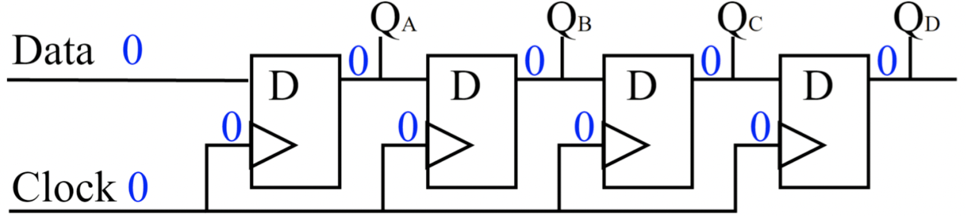
\includegraphics[width=0.5\textwidth]{images/banch_of_flipflops.png}
	\caption{Banch of electronic flipflops.} \label{fig:banch_of_flipflops}
\end{figure}

The circuit can be made to change state by signals applied to one or more
control inputs and will have one or two outputs. It is the basic storage element
in sequential logic. Flip-flops and latches are fundamental building blocks of
digital electronics systems used in computers, communications, and many other
types of systems.

A flip-flop is a device which stores a single bit (binary digit) of data; one of
its two states represents a ``one" and the other represents a ``zero". Such data
storage can be used for storage of state, and such a circuit is described as
sequential logic in electronics. When used in a finite-state machine, the output
and next state depend not only on its current input, but also on its current
state (and hence, previous inputs). It can also be used for counting of pulses,
and for synchronizing variably-timed input signals to some reference timing
signal.

Flip-flops can be either level-triggered (asynchronous, transparent or opaque)
or edge-triggered (synchronous, or clocked). The term flip-flop has historically
referred generically to both level-triggered and edge-triggered circuits that
store a single bit of data using gates. We will refer Flip-Flop as
edge-triggered i.e. clocked synchronized.

Flip-flop has to legs – data and clock, for each storage element in the circuit
the data changes at the clock signal and so we have an amplified signal that we
can monitor as attackers and try to learn the secret behind it.

 \subsection { Core I7 chip }
 
Following is the core I7 chip image:

\begin{figure}[!ht]
	\centering
	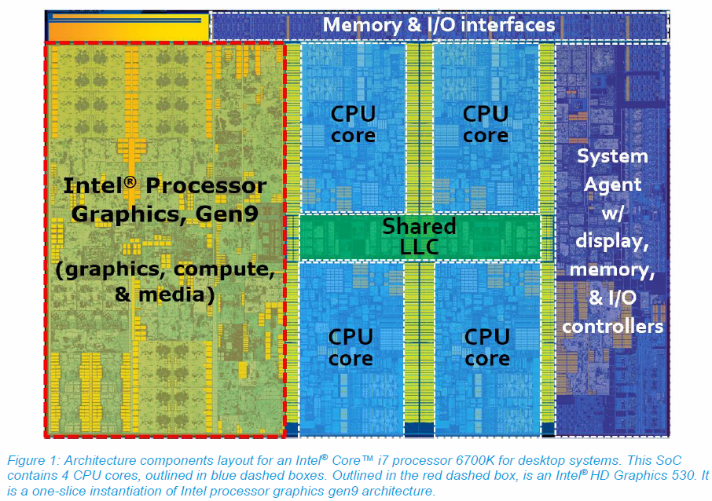
\includegraphics{images/i7.png}
	\caption{Intel i7.} \label{fig:i7}
\end{figure}

We can see ordered items that are the storage elements, there are 24 items that
are the GPUs and they have a little memory next to the (upper left). The CPU
core has also a cash memory in it.

\subsection { Power Consumption is Variable }

Next we will see how to get secrets from the power consumption.

\begin{figure}[!ht]
    \centering
    \tikzset{every picture/.style={line width=0.75pt}} %set default line width to 0.75pt        
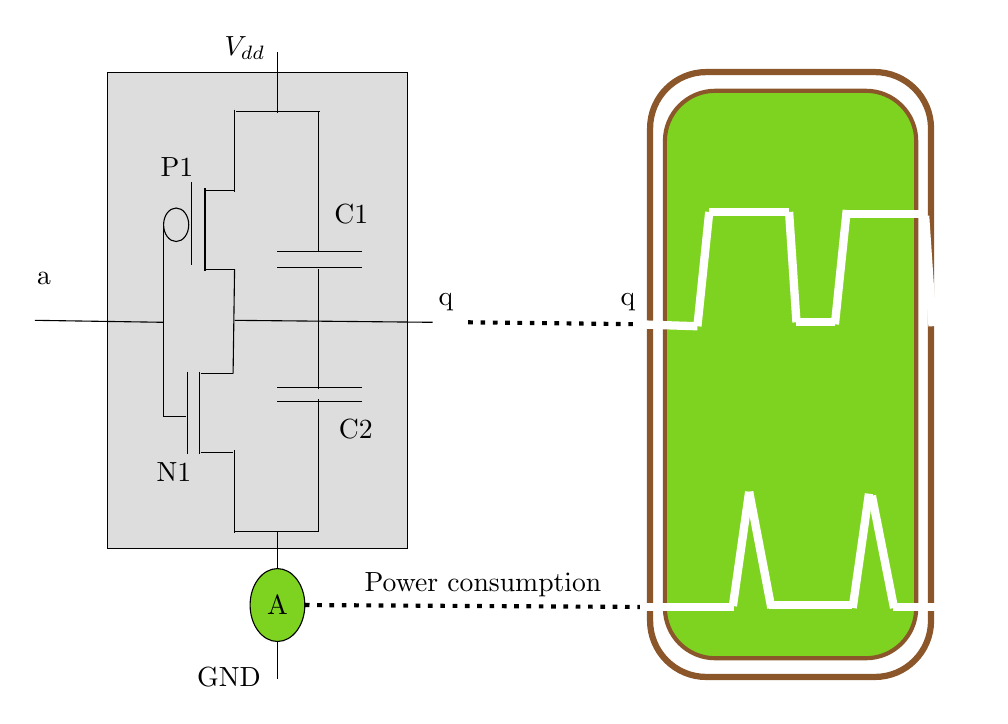
\begin{tikzpicture}[x=0.75pt,y=0.75pt,yscale=-1,xscale=1]
%uncomment if require: \path (0,335); %set diagram left start at 0, and has height of 335

%Shape: Rectangle [id:dp0360003318411668] 
\draw  [fill={rgb, 255:red, 207; green, 207; blue, 207 }  ,fill opacity=0.71 ] (39.45,26.06) -- (184.07,26.06) -- (184.07,255.79) -- (39.45,255.79) -- cycle ;
%Straight Lines [id:da9130268694115924] 
\draw    (4.54,145.67) -- (66.52,146.62) ;


%Straight Lines [id:da1343440150952362] 
\draw    (66.52,98.21) -- (66.52,192.18) ;


%Shape: Ellipse [id:dp6213874655305351] 
\draw   (72.57,91.56) .. controls (75.92,91.56) and (78.63,95.17) .. (78.63,99.63) .. controls (78.63,104.09) and (75.92,107.7) .. (72.57,107.7) .. controls (69.23,107.7) and (66.52,104.09) .. (66.52,99.63) .. controls (66.52,95.17) and (69.23,91.56) .. (72.57,91.56) -- cycle ;
%Straight Lines [id:da27434486206672837] 
\draw    (66.52,192.18) -- (77.2,192.18) ;


%Straight Lines [id:da07016771982069758] 
\draw    (77.92,170.35) -- (77.92,210.22) ;


%Straight Lines [id:da19036973562649373] 
\draw    (83.62,170.35) -- (83.62,210.22) ;


%Straight Lines [id:da8345791716423674] 
\draw    (80.05,79.22) -- (80.05,119.09) ;


%Straight Lines [id:da3271159414725533] 
\draw    (86.47,82.07) -- (86.47,121.94) ;


%Straight Lines [id:da14873596785352006] 
\draw    (84.33,209.27) -- (100,209.27) ;


%Straight Lines [id:da4420681124736481] 
\draw    (84.33,171.3) -- (100,171.3) ;


%Straight Lines [id:da04393107109208283] 
\draw    (87.18,120.99) -- (100.72,120.99) ;


%Straight Lines [id:da3871143133174997] 
\draw    (87.18,83.02) -- (100.72,83.02) ;


%Straight Lines [id:da5151381716842007] 
\draw    (100.72,120.99) -- (100,171.3) ;


%Straight Lines [id:da6069121794097094] 
\draw    (100.72,44.1) -- (100.72,83.97) ;


%Straight Lines [id:da2848668560084322] 
\draw    (100.72,208.32) -- (100.72,248.19) ;


%Straight Lines [id:da29161700195638374] 
\draw    (101.43,45.05) -- (142.04,45.05) ;


%Straight Lines [id:da2980631065657684] 
\draw    (100.72,247.24) -- (141.32,247.24) ;


%Straight Lines [id:da3565336880454746] 
\draw    (141.32,45.05) -- (141.32,112.45) ;


%Straight Lines [id:da47251450500555436] 
\draw    (141.32,183.64) -- (141.32,247.24) ;


%Straight Lines [id:da3833560512127223] 
\draw    (121.38,184.59) -- (161.98,184.59) ;


%Straight Lines [id:da8160698305270608] 
\draw    (121.38,177.95) -- (161.98,177.95) ;


%Straight Lines [id:da053729746303400994] 
\draw    (121.38,112.45) -- (161.98,112.45) ;


%Straight Lines [id:da6110612216423352] 
\draw    (121.38,120.04) -- (161.98,120.04) ;


%Straight Lines [id:da24663417263394583] 
\draw    (141.32,120.99) -- (141.32,178.9) ;


%Straight Lines [id:da6538334507705081] 
\draw    (100.72,145.67) -- (196.18,146.62) ;


%Straight Lines [id:da6610435045454974] 
\draw    (121.38,16.57) -- (121.38,46) ;


%Straight Lines [id:da11217271094658177] 
\draw    (121.38,247.24) -- (121.38,265.28) ;


%Shape: Ellipse [id:dp5116375931959476] 
\draw  [fill={rgb, 255:red, 126; green, 211; blue, 33 }  ,fill opacity=1 ] (108.2,282.84) .. controls (108.2,273.14) and (114.1,265.28) .. (121.38,265.28) .. controls (128.65,265.28) and (134.56,273.14) .. (134.56,282.84) .. controls (134.56,292.54) and (128.65,300.4) .. (121.38,300.4) .. controls (114.1,300.4) and (108.2,292.54) .. (108.2,282.84) -- cycle ;
%Straight Lines [id:da9407053227115245] 
\draw    (121.38,300.4) -- (121.38,318.44) ;


%Rounded Rect [id:dp5069309881092712] 
\draw  [color={rgb, 255:red, 139; green, 87; blue, 42 }  ,draw opacity=1 ][line width=2.25]  (300.91,53.14) .. controls (300.91,38.18) and (313.03,26.06) .. (327.98,26.06) -- (409.2,26.06) .. controls (424.15,26.06) and (436.27,38.18) .. (436.27,53.14) -- (436.27,290.42) .. controls (436.27,305.37) and (424.15,317.49) .. (409.2,317.49) -- (327.98,317.49) .. controls (313.03,317.49) and (300.91,305.37) .. (300.91,290.42) -- cycle ;
%Rounded Rect [id:dp10813466593651544] 
\draw  [color={rgb, 255:red, 139; green, 87; blue, 42 }  ,draw opacity=1 ][fill={rgb, 255:red, 126; green, 211; blue, 33 }  ,fill opacity=1 ][line width=1.5]  (308.05,59.3) .. controls (308.05,45.92) and (318.89,35.08) .. (332.27,35.08) -- (404.91,35.08) .. controls (418.29,35.08) and (429.13,45.92) .. (429.13,59.3) -- (429.13,284.26) .. controls (429.13,297.63) and (418.29,308.47) .. (404.91,308.47) -- (332.27,308.47) .. controls (318.89,308.47) and (308.05,297.63) .. (308.05,284.26) -- cycle ;
%Straight Lines [id:da10126802822138314] 
\draw [line width=1.5]  [dash pattern={on 1.69pt off 2.76pt}]  (213.28,146.62) -- (298.77,147.57) ;


%Straight Lines [id:da8166666674599945] 
\draw [line width=1.5]  [dash pattern={on 1.69pt off 2.76pt}]  (134.56,282.84) -- (301.26,283.79) ;


%Straight Lines [id:da6599388820944971] 
\draw [color={rgb, 255:red, 255; green, 255; blue, 255 }  ,draw opacity=1 ][line width=3]    (294.5,147.57) -- (323.71,148.52) ;


%Straight Lines [id:da6477850565472385] 
\draw [color={rgb, 255:red, 255; green, 255; blue, 255 }  ,draw opacity=1 ][line width=3]    (323.71,148.52) -- (329.41,93.46) ;


%Straight Lines [id:da6713764130615041] 
\draw [color={rgb, 255:red, 255; green, 255; blue, 255 }  ,draw opacity=1 ][line width=3]    (329.41,93.46) -- (367.88,93.46) ;


%Straight Lines [id:da6265334534856528] 
\draw [color={rgb, 255:red, 255; green, 255; blue, 255 }  ,draw opacity=1 ][line width=3]    (371.44,146.62) -- (367.88,93.46) ;


%Straight Lines [id:da7580446433818473] 
\draw [color={rgb, 255:red, 255; green, 255; blue, 255 }  ,draw opacity=1 ][line width=3]    (371.44,146.62) -- (389.96,146.62) ;


%Straight Lines [id:da12760629606366103] 
\draw [color={rgb, 255:red, 255; green, 255; blue, 255 }  ,draw opacity=1 ][line width=3]    (389.96,147.57) -- (395.66,92.51) ;


%Straight Lines [id:da35722507690924] 
\draw [color={rgb, 255:red, 255; green, 255; blue, 255 }  ,draw opacity=1 ][line width=3]    (394.95,94.41) -- (433.42,94.41) ;


%Straight Lines [id:da9407492544795262] 
\draw [color={rgb, 255:red, 255; green, 255; blue, 255 }  ,draw opacity=1 ][line width=3]    (436.98,148.52) -- (433.42,95.36) ;


%Straight Lines [id:da36688349354965344] 
\draw [color={rgb, 255:red, 255; green, 255; blue, 255 }  ,draw opacity=1 ][line width=3]    (296.28,283.79) -- (341.16,283.79) ;


%Straight Lines [id:da07990995883843] 
\draw [color={rgb, 255:red, 255; green, 255; blue, 255 }  ,draw opacity=1 ][line width=3]    (340.8,283.31) -- (348.64,228.26) ;


%Straight Lines [id:da7808057757591158] 
\draw [color={rgb, 255:red, 255; green, 255; blue, 255 }  ,draw opacity=1 ][line width=3]    (359.33,284.26) -- (348.64,228.26) ;


%Straight Lines [id:da6401094233638194] 
\draw [color={rgb, 255:red, 255; green, 255; blue, 255 }  ,draw opacity=1 ][line width=3]    (358.26,282.84) -- (398.16,282.84) ;


%Straight Lines [id:da0933201425519079] 
\draw [color={rgb, 255:red, 255; green, 255; blue, 255 }  ,draw opacity=1 ][line width=3]    (398.51,284.26) -- (406.35,229.21) ;


%Straight Lines [id:da038966229239766115] 
\draw [color={rgb, 255:red, 255; green, 255; blue, 255 }  ,draw opacity=1 ][line width=3]    (418.46,284.26) -- (407.77,230.16) ;


%Straight Lines [id:da29582365028992696] 
\draw [color={rgb, 255:red, 255; green, 255; blue, 255 }  ,draw opacity=1 ][line width=3]    (418.1,283.79) -- (458,283.79) ;



% Text Node
\draw (8.81,125.74) node  [align=left] {a};
% Text Node
\draw (72.93,71.63) node  [align=left] {P1};
% Text Node
\draw (71.51,218.76) node  [align=left] {N1};
% Text Node
\draw (157,94.41) node  [align=left] {C1};
% Text Node
\draw (159.13,197.88) node  [align=left] {C2};
% Text Node
\draw (121.38,282.84) node  [align=left] {A};
% Text Node
\draw (202.59,137.13) node  [align=left] {q};
% Text Node
\draw (290.22,137.13) node  [align=left] {q};
% Text Node
\draw (220.4,272.87) node  [align=left] {Power consumption};
% Text Node
\draw (97.99,317.74) node  [align=left] {GND};
% Text Node
\draw (105.7,14.67) node  [align=left] {$\displaystyle V_{dd}$};


\end{tikzpicture}
    \caption{Not gate connected to an oscilloscope.} \label{fig:Not gate connected to an oscilloscope}
\end{figure}

This is the NOT gate as before connected with an ampere meter so we can measure
the power consumption, also there are two capacitors (C1 \& C2). The capacitors
are connected because the characteristics of the circuit which make it to act
like capacitors. They are not transferring current but they will have an effect
on the math we are going to do next.

Next we are taking a square wave, which looks like this:

And we have to feed it into the NOT gates, the output is going to be the
opposite of the square wave, and we want to measure the power consumption using
an oscilloscope. The x axis of the oscilloscope is time and the y axis in this
case it's a voltage of the power. It's a current moving across the ampere meter.
What we can see here is that when the circuit is stable, there was not much
power consumption, but when the system is switching, when there is a high power
consumption, because there is a glitch when one transistor is opening and the
other one is closing. Also, we can see that the lines in the oscilloscope are
not having the same size as the capacitors are actually charging and discharging
without we want it. We can learn from this if there was one or zero and what is
the rate of switching, and we can store this information.

The power consumption is the sum of the statistic and the dynamic power
consumption: 

\begin{displaymath}
    P(t)=P_{stat}(t) + P_{dyn}(t)
\end{displaymath}

We don't care about the statistic power consumption as it is just defined by the
kind of silicone that we are using, the size of the features decided to be in
the transistors, the temperature, the technology, etc. But really interesting
for us is the dynamic power consumption that depends on the o'clock rate and the
circuit activity input data.

Because the power consumption is a function of the circuit activity, we can try
to measure the power consumption and send the results to the equations and to
get the circuit activity, in a way we can find out all the secrets.

In order to calculate the power consumption this way we need a lots of data
about the circuit and about the environment and about the temperature etc. And
this is too much work for us as an engineers. There is a much simplified way of
measuring the power consumption of a device, assuming it's a CMOS device we can
measure how many bits changes every clock.

So, our assumptions are the followings:
\begin{inparaenum}
    \item This is a CMOS device.
    \item When it's static the static power is very low, and when it switches,
    there is a very high power consumption.
    \item This is synchronous circuit, which means it has a lot of flip flops
    that all change at the same time.
    \item The power consumption is proportional to the amount of changes and the
    outputs of these flip flops.
\end{inparaenum}


\subsection { hamming distance model }

For doing this we are going to use hamming distance model. The Hamming distance
between two vectors is the number of bits we must change to change one into the
other. Example, what is the distance between the vectors 01101010 and 11011011? 

\begin{displaymath}
    X=x_{n},x_{n-1},...,x_{1},x_{0}
\end{displaymath}
Hamming weight:
\begin{displaymath}
    HW(X)=\sum x_{i}
\end{displaymath}
Hamming distance: 
\begin{displaymath}
    HD(X,Y)=HW(V_{1} \bigoplus V_{2})
\end{displaymath}
Answer: They differ in four places, so the Hamming distance d(01101010,11011011)
= 4.

When talking about CMOS devices we are estimating our power consumption as
amount of bits (transitions) that change from one to zero or from zero to one,
this is our hamming distance. By monitoring the changes as explained we can find
the power consumption.

But, this is not enough. By connecting the oscilloscope to our device we are
trying to measure a physical device with another physical equipment, and what
they are measuring is subject to measurement errors like switching noise,
thermal noise and measurement noises.

Switching noise means that there are other kinds of activity which are going on
in the circuit in addition. Measurement noise means that our desk setup is not
always accurate, or we might be connected not properly, or we might not be
measuring the precise correct moment of time etc. Thermal noise - we are
measuring electrical activity, as electrons are very crazy particles and they
like to disappear and reappear in a nearby location. So the higher is the
temperature, the more likely they are to vanish and disappear. And when the
electrons are moving, they generate radiation and they affect our measurements.

So now when we are measuring the power, we get the static power, the dynamic
power and we get the noise:

\begin{displaymath}
    P_{meas}(t)=P_{stat}(t) + P_{dyn}(t) + N(t)
\end{displaymath}

In order to avoid the noise we can measure it again and again and then the noise
might be canceling itself. What happens sometimes is that the noise, especially
the switching noise, is sometimes correlated with the activity of the circuits.
Another thing we can do is controlling the noise somehow like running our
experiment inside a freezer, or an isolated environment where there's no
electric noise around. We can also, open the dives and try to kill the sources
of noise.

That's one very nice thing we can do is instead of measuring power consumption,
we can measure electromagnetic radiation. And this has two advantages, first of
all, it's less invasive and second of all, it can be focused and, and reduce the
switching noise.

\subsection { From Power to Electromagnetic }

\begin{figure}[!ht]
    \centering
    \tikzset{every picture/.style={line width=0.75pt}} %set default line width to 0.75pt        

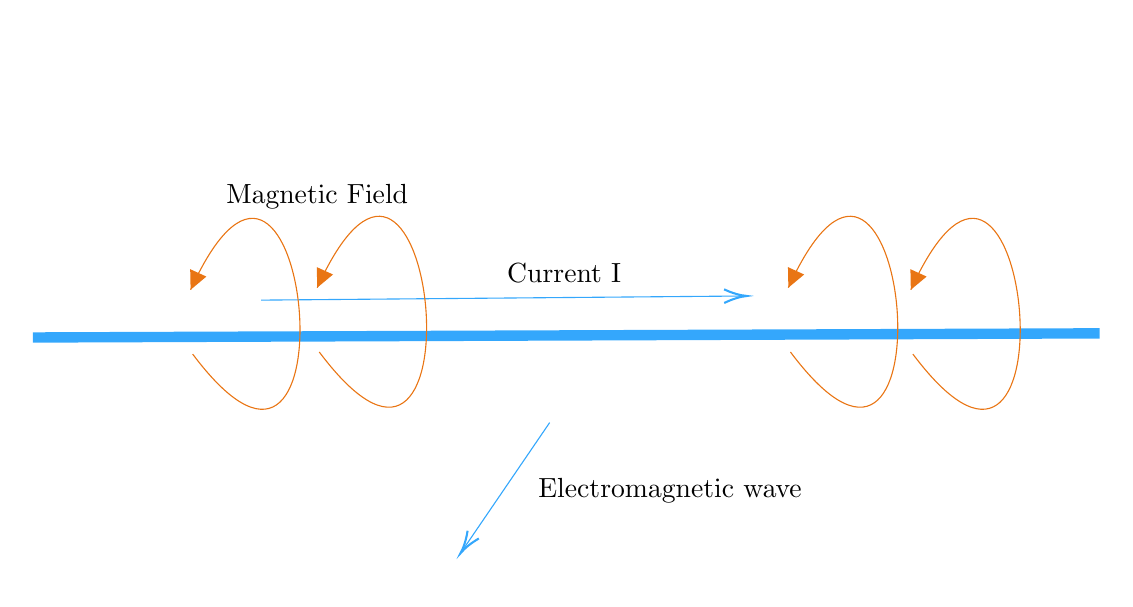
\begin{tikzpicture}[x=0.75pt,y=0.75pt,yscale=-1,xscale=1]
%uncomment if require: \path (0,300); %set diagram left start at 0, and has height of 300

%Straight Lines [id:da730115903310417] 
\draw [color={rgb, 255:red, 52; green, 167; blue, 252 }  ,draw opacity=1 ][line width=3.75]    (69,171) -- (583,169) ;


%Straight Lines [id:da8949672238779289] 
\draw [color={rgb, 255:red, 52; green, 167; blue, 252 }  ,draw opacity=1 ]   (179,153) -- (411,151.02) ;
\draw [shift={(413,151)}, rotate = 539.51] [color={rgb, 255:red, 52; green, 167; blue, 252 }  ,draw opacity=1 ][line width=0.75]    (10.93,-3.29) .. controls (6.95,-1.4) and (3.31,-0.3) .. (0,0) .. controls (3.31,0.3) and (6.95,1.4) .. (10.93,3.29)   ;

%Curve Lines [id:da4084322101826783] 
\draw [color={rgb, 255:red, 233; green, 117; blue, 20 }  ,draw opacity=1 ]   (493,179) .. controls (574,287) and (549,23) .. (492,148) ;
\draw [shift={(492,148)}, rotate = 294.51] [fill={rgb, 255:red, 233; green, 117; blue, 20 }  ,fill opacity=1 ][line width=0.75]  [draw opacity=0] (8.93,-4.29) -- (0,0) -- (8.93,4.29) -- cycle    ;

%Straight Lines [id:da8207423009134964] 
\draw [color={rgb, 255:red, 52; green, 167; blue, 252 }  ,draw opacity=1 ]   (318,212) -- (276.13,273.35) ;
\draw [shift={(275,275)}, rotate = 304.32] [color={rgb, 255:red, 52; green, 167; blue, 252 }  ,draw opacity=1 ][line width=0.75]    (10.93,-3.29) .. controls (6.95,-1.4) and (3.31,-0.3) .. (0,0) .. controls (3.31,0.3) and (6.95,1.4) .. (10.93,3.29)   ;

%Curve Lines [id:da43215348815507637] 
\draw [color={rgb, 255:red, 233; green, 117; blue, 20 }  ,draw opacity=1 ]   (434,178) .. controls (515,286) and (490,22) .. (433,147) ;
\draw [shift={(433,147)}, rotate = 294.51] [fill={rgb, 255:red, 233; green, 117; blue, 20 }  ,fill opacity=1 ][line width=0.75]  [draw opacity=0] (8.93,-4.29) -- (0,0) -- (8.93,4.29) -- cycle    ;

%Curve Lines [id:da7658292921428724] 
\draw [color={rgb, 255:red, 233; green, 117; blue, 20 }  ,draw opacity=1 ]   (146,179) .. controls (227,287) and (202,23) .. (145,148) ;
\draw [shift={(145,148)}, rotate = 294.51] [fill={rgb, 255:red, 233; green, 117; blue, 20 }  ,fill opacity=1 ][line width=0.75]  [draw opacity=0] (8.93,-4.29) -- (0,0) -- (8.93,4.29) -- cycle    ;

%Curve Lines [id:da6169102709245924] 
\draw [color={rgb, 255:red, 233; green, 117; blue, 20 }  ,draw opacity=1 ]   (207,178) .. controls (288,286) and (263,22) .. (206,147) ;
\draw [shift={(206,147)}, rotate = 294.51] [fill={rgb, 255:red, 233; green, 117; blue, 20 }  ,fill opacity=1 ][line width=0.75]  [draw opacity=0] (8.93,-4.29) -- (0,0) -- (8.93,4.29) -- cycle    ;


% Text Node
\draw (206,103) node  [align=left] {Magnetic Field};
% Text Node
\draw (325,140) node  [align=left] {Current I};
% Text Node
\draw (376,245) node  [align=left] {Electromagnetic wave};


\end{tikzpicture}


    \caption{electromagnetic emission.} \label{fig:electromagnetic emission}
\end{figure}

Electric fields are created by differences in voltage: the higher the voltage,
the stronger will be the resultant field. We can use the right hand rule in
order to remember the direction of the electromagnetic field direction when we
know the current direction. We can measure the magnetic field, but one
disadvantage is that it is very localize, so we need to get access to the
device. We can connect an antenna to the device and then we can measure the
electromagnetic wave using a receiver. There is a very nice paper called
screaming channels where you can read more about this kind of attacks.


\chapter{Low Data Complexity Power/EM 2}

We want to see what is power analysis all about and see a very simple power
analysis attack that we can actually perform. Then we will dive into AES and its
implementation.

All the things that we will see today are very optimistic and they assume that
we have really good measurements, very good understanding and very good luck,
but it's actually quite a little bit harder in practice.

\section{The New York Times, Take 2}
The hero for this article is Mister Kocher. He discovered something that can
attack smart cards with what's called power analysis. Probably it was discovered
before, but he has discovered it academically.

What did he do? He went to a conference and took people's smart cards and found
out their secret private keys. We saw last week that if we have to sign
something and we have the private key you can sign a thing that's not supposed
to be signed and steal money, this was a big deal.

The 1995 timing attack went to the front page of the New York Times and there
was a lot of discussion about the discovery. The 1998 result about power
analysis only goes to the bottom of page two in one of the supplements and
actually nobody has discussed about it a lot. 

Why didn't he get a lot of attention for this power analysis attack? Could be
because timing is one thing and power analysis is a little more complicated but
in the bottom line we can see all the secrets. To do a timing attack you need a
stopwatch, while to power analysis attack you need more sophisticated equipment.

\section{Power Analysis Attacks}
What we need to make timing attack? We just need to be able to send request and
gets responses to measured how much it took, while the target can be at the
other side of the internet (can Amazon Cloud very far away).

What we need to make Power analysis attack? We need to be physically. How do we
connect to the device? We need to cut the power supply and connect to it
diractly to measure the power consumption. This is a very invasive attack, we
need to be very very close. in 1995 let's assume that it's true. so if we go to
the system architect:” listen there is an a power analysis attack that's can
completely compromised the device. Attacker needs to come to the device end cuts
the power supply….” by the time you already lost the system architect because
this is not practical. The threat model has to make sense.
 
nevertheless, the threat model does make sense in a lot of scenarios and we
discovered that thing that we was not supposed existing these power analysis and
side Channel attack. today we can attack this device and tomorrow we can attack
another device.

To learn about power analysis attack you can go and search in the library the
“Power Analysis Attacks” book.“Cryptanalytic attacks that allow extraction of
secret information from cryptographic devices by exploding their power
consumption characteristics”let's see what can we discover from this definition.
First, What we are attacking here? Cryptographic devices. what we are not
attacking? cryptographic algorithms. If I told you that I was able to break RSA
on my phone by doing power analysis did I break RSA? No we didn't break RSA, we
break the implementation of RSA. What else we are not attacking? The user is not
under attack, we are not doing any key logging or human engineering attack or
social engineering we are only attacking the device. What's the cryptographic
device? Some kind of crypto, signing or encrypting. What a secret information we
wants to extract? Probably we extract the key. And what's nice about the key?
That he has lots of bits. At the start you don't know anything about the key, If
you get half of the key you halfway, if you get the whole key You win. If I want
to make the device more secure what do I need to do to key? we make a longer
key.

This is very easy to say, but if I'm talking instead of secret information we
cracked from the device, like medical information, it's a little harder to
understand what we can do with half of it. How do we make the medical
information more secure? What it's actually means?

Let's take credit cards, the companies say that you are more secure with credit
card. Why do we think that we have a privacy with credit cards? We are giving
the credit card number and our name... Looks like we're giving everything, the
saying that we are actually have privacy, a lot of people have in the US have
the same name, but you also get a zip code. Every time you pay with the credit
card it generate a new credit card number automatically and doesn't have any
digits on him. It is very hard to talk about privacy if it's not a
cryptographic. What's left from the definition? we are exploiting the power
conceptions characteristic.

What are we not exploiting? We're not doing math and we are not doing something
that you can do by algorithms. It's important to know that exploiting the power
at conception characteristics does not have to be actually measuring the power.
We saw last week that we can actually measure the power consumption with other
methods. When Kotcher wrote his paper he announced three types of power
analysis. One of them called Simple power analysis, the other one called
differential power analysis. Let's see the simple power analysis today.

\section{Simple Power Analysis}

The simple power analysis means that I'm going to take the measurement of the
device, making one measurement or two. With that we are going to get the key
from those measurement. What's nice about this attack that it's very reasonable
attack model. We need to get the power consumption trace ( this is a vector
overtime of the power consumption of the device), and we need only one or two
traces. This is actually durable in a lot of scenarios even if I have the device
for a little time or even if someone is looking at me. We will see the setup
that can be used for simple analysis. 

When you go to a store in Europe, you can't give the credit card for the
cashier, they give you this terminale and then you need take your credit card
insert it and put the pin number. And what is going over here, there is
something like a cryptographic computer between your card and terminal. Let's
assume that we want to attack the card, and it is in my possession. This model
is very permissive to me and I can do whatever I want, I can do a lot of
transactions I can do radiat, I can twist it and even melt it. so attacking the
card is very easy.


But if I don't wants to attack the card? I want to attack the terminal using
power analysis. Maybe the terminal has an SSL private key which is used to
connect to the Central Center, and this can make a lot of damage and we can be
very rich.

We want to do a power analysis on the terminal. This is a nice setup, this is
something that looks like a credit card, but it has are wired connected to this
fpga and connect to a computer. I will be in a very cold country and I will take
this card out from the jacket to my palm. Insert this chip into the terminal,
while doing a power analysis on a this terminal. The idea is that I can do it
about 1 or two times, but not making it for a thousand times or melt it. I can
attack maybe this terminal or a gas station. The fact that we don't need a lot
of traces is actually good.

What are the disadvantages? The problem here is that when I look at this power
trace I need to be very very well prepared, and understand what's really going
on in the power trace. Because we get a vector with a hundred thousand points
and we need to understand where is the encryption starting? Where it is ending?
What it means that there is a lack of power here a little power there? We need
to have a very good understanding of the device processes. 

Not only that we need also to have a very good measurements, because I only have
one or two measurements. They're a lot of external Influence on the device,
there can be noise, may be related to the device may be related to the
environment, and if I have only one measurement I am going to get all of this
noise at once and cannot do anything to reduce it. Statistically I'am not going
to be able to get clean measurements to perform the attack.

Another problem is that I will need to work very hard to find the key. Let see
an example: Yossi did a power analysis measurements and he got a Trace and there
was a noise, he did his analysis and got the key. Now he want to check if this
is the right key. How can we check the key? Try to decrypt and encrypt the
private key. Is this the right key? no it's not :( .. Why? We have only one
Trace. Maybe there was noise? Maybe one measurement was wrong? How do we recover
from this? We can try a similar key and not there exact key, maybe to change you
on bit here or there. This search might be so intensive that we getting
basically the same effect like a Brute Force. This makes simple power analysis
are not very effective because of all of those reasons.

\section{Other Types of Power Attacks}

So in general in power analysis there are two classes:

\paragraph{Low data complexity attacks} where I get line trace or two traces (a
very small amount of traces). Then I do a lot of post-processing and think
really really hard and maybe do a reverse engineering before.

\paragraph{High data complexity attacks} I will talk to you about it next week.
These attacks require a lot of traces, maybe thousands or Millions traces, a
Terabyte of data.

\section{Tuning the power model}

 The first thing that you need to do for a simple power analysis attack is to
 understand what device you are attacking. We attack two general types of
 devices with simple power analysis, first is a microcontroller or a CPU and the
 other thing is ASIC. 
 
Microcontroller is basically a regular computer, it gets commands and runs it
one after another, if you want to write a new software for this computer you can
write it in C or Java, they're cheap and commonly used.

\begin{figure}[htp]
\hspace*{0in}
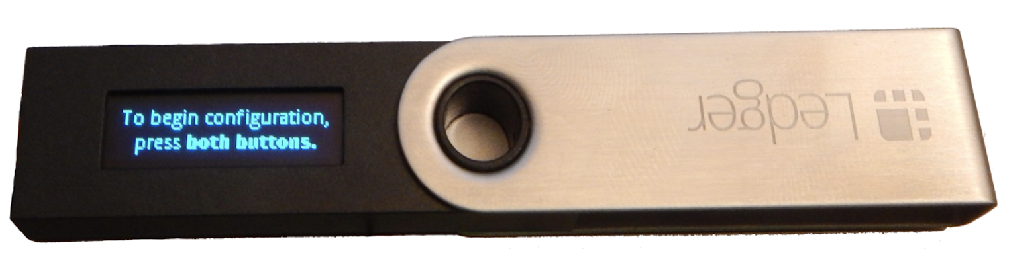
\includegraphics[scale=0.3]{images/Lecture_5/ledger.png}
\caption{Bitcoin Wallet}\label{fig:Bitcoin Wallet}
\end{figure}

This is a Bitcoin wallet. The Bitcoin is basically numbers and if someone steals
these numbers he steals your money, so you don't want these numbers to be on
your computers. These do all the calculation when you connect to the network, we
want it to be very secure because if someone steal the secret key he can take
all of your money.

\paragraph{}
Inside this device it has an orange Square and this is the microcontroller. Her
some storage and you can write some code for it.

The other kind of a device is called ASIC, this device is manufactured only for
a specific purpose. Let's say I want to have a sprinkler that starting the
morning and ends in the evening, I will use a programming language that called
HDL, once I compiled these software I am not getting an executable program that
I can run on a device. These chips can only do one thing, I can't programming
them and I can't upgrade them, if there is a bug I am in a big problem, but they
have only one purpose. The power consumption of this devices are going to be
smaller and sometimes they even be faster. Microcontrollers have programs that
runs one line after another, an ASIC can do a parallel operation. ASIC is very
cheap to manufacture, but there is a big wrap up before you produced this.

In this course we are going to talk only about microcontrollers, because we are
going to see them more often than ASICs. But you will know enough to open the
book attacking ASIC.


\begin{figure}[htp]
\hspace*{0in}
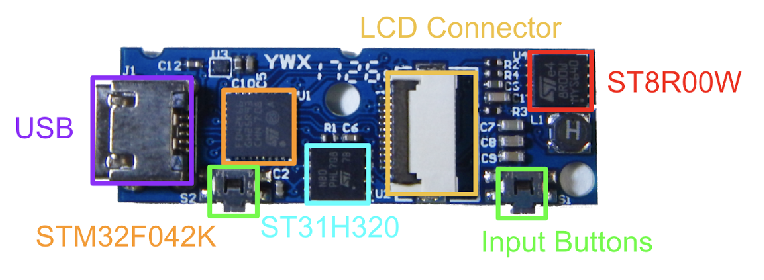
\includegraphics[scale=0.4]{images/Lecture_5/arduino.png}
\caption{Arduino}\label{fig:Arduino}
\end{figure}

So what is the line between microcontroller and an ASIC? On one of the student
table there is a chip that he will show us, this is a FPGA field programmable
this chip. If I want to identify a particular face I can program this ASIC to do
patterning for this face and doing it very very cheaply. I can do also audio
compression maybe I don't know what exactly I want to do but I know that I need
to do some kind of compression while I don't know exactly the algorithm by using
this ASIC. So you will find an ASIC if you have a piece of equipment 10000
pieces, maybe a router ,oscilloscope, submarine and things like that. Best to
make sure what is an Arduino? Microcontroller. 


\section{8-bit microcontroller}

This is an 8-bit microcontroller from the 80s, you see the center of this
microcontroller , this pair of trousers the red that named ALU, this is where
the magic happens, this piece of silicone can actually do logic like multiply,
add, shift or compare. 

\begin{figure}[htp]
\hspace*{0in}
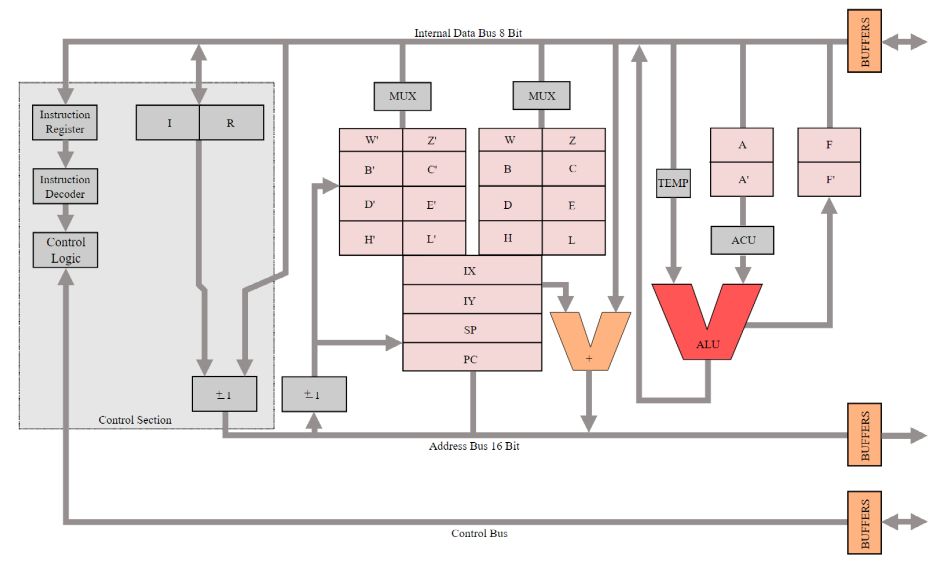
\includegraphics[scale=0.3]{images/Lecture_5/8bit-mc.png}
\caption{8-bit microcontroller}\label{fig:8-bit microcontroller}
\end{figure}


The entire process of life is to get a line of code which represent an
instruction, he has to understand what this instruction is trying to do. It can
be multiply, read or write. And then you get the operator you need to do from
the memory and fed it to the ALU. Then we'll get the next instruction and we'll
do it again and again. what's important for me to show you that there is two
long in lines from the top and the bottom they are called the buses. the top
called the data bus and the bottom call address bus. What is data bus mean? Any
sort of data you need to computation has to fetch from this bus. If something
come from the memory it going from this bus. If I want to write to external
input output, it also going on this bus. The width of this bus is 8 Bits and it
means all of the operation that this microcontroller do our eight bits.

On the bottom there is another big bus which is the address bus. If I want to
write to memory, I'm going to put their address in the address bus and then I'm
going to put the data in the data bus. I will set the control bus to write, and
then the memory which is somewhere else is it going to rise to this address. If
I want to do a read, I will put the address I want to read in the address bus,
and read in the control. What I will do in the data bus? I don't want to put
something in there because I want to read, this is actually important and I will
elaborate about it more later.

\section{Power Model for Microcontrollers}
What's interesting about microcontroller that there are in many cases the power
model don't have Hamming distance and actually have Hamming Weight. What does
that mean? That if I think that there are going to be a value going over the bus
I don't need to know what was the previous value on the bus, because it's going
to be exact humming weight for this value. 

When you have the best that is shared with several components the idea is that
all of the components that are not using the bus are going to set how to put
them, so all are ones, So if I want for example to read advice from memory the
CPU is going to set everything to one and then he is going to extract the memory
from the address, then the memory is going to lower all the relevant bits until
what sitting on the memory bus and the data bus what I wanted. 

Let's say I want the memory 4, at first I'm going to see on the data bus 0xFF,
then I will see 4 and then going to see agaoxin FF because the memory is
finished. what was the power-consumption here to go from FF to 4, how many beats
has to change? 7, and again it goes back to FF.

\section{Simple Power Analysis of RSA}
Let's see the power module this device under test, which does RSA decryption or
signing. While it's doing it we are getting the power measures. Why it is doing
an RSA decryption? Because it needs it. We can do it by sending encrypted emails
from the phone, so you really have to decrypt the message.

\begin{figure}[htp]
\centering
\hspace*{0in}
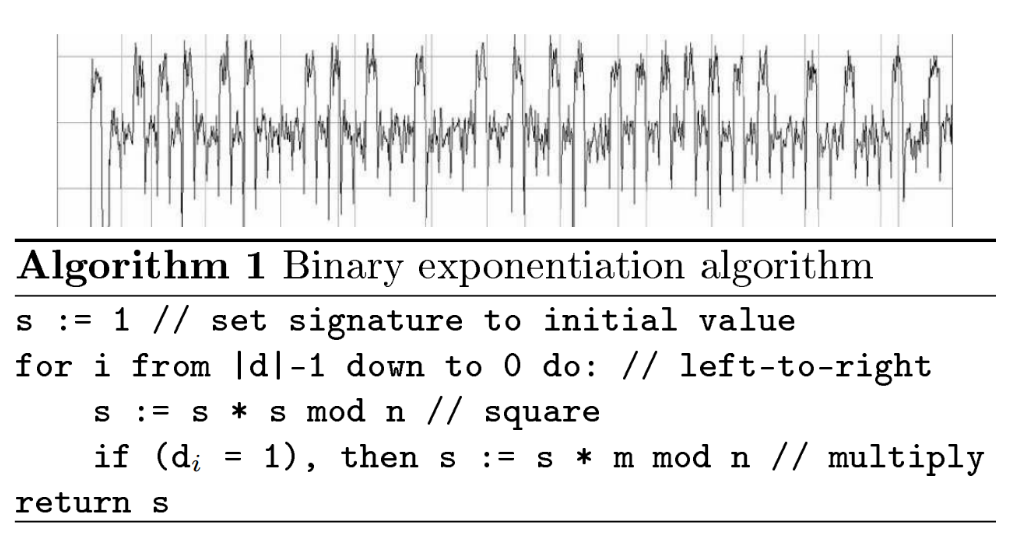
\includegraphics[scale=0.3]{images/Lecture_5/RSA-PA.png}
\caption{RSA Power Analysis}\label{fig:RSA Power Analysis}
\end{figure}

The axis are vector of power measurements, x is time, y are the power
consumption,(how did we measure the power consumption? i put a probe, measer the
voltege so on.. What is the private key? What is missing? You need to do some
reverse engineering first. If this is the only chance to get the key, I need to
tell you a little bit more about the device so you will understand what is going
on here. This device is microcontroller, it's doing RSA decryption using right
to left binary exponentiation using square and multiply. Is it helping you
finding the key? Yes. Let me show you the source code.

Binary exponentiation, it starts from the top most bit, off the secret and
privates decryption key, and then for each bit we do Square and multiply. If the
bit is zero we do Square, if this bit is one we do square and multiply. This
help you now finding the key, let's look at that Power Trace.

We see two types of things here, this little thing and the big thing. We have
some little thing, big thing, little thing, big thing, and then little little
little, and then big thing.

All we need to do is to be able tell about were is the square and were is
multiply, and then I can read the key, from top to bottom. So telling about
square and the multiply to get to the key is the general method. We see square
is take a little power and multiply more power.

What is square? square is multiply. So why is the power consumption of square
using multiply is different? this is a microcontroller and his bus width is 8
bit. He's doing a convolution between numbers, so it's multiply thousands of
time in frame. so why this is different? So what is consuming power, the ALU is
consumer power, the data bus and the address bus consuming power. In this case
the power consumption module of the address bus is hemming distance, because
it's not setting to 1 between accesses it's always containing what CPU is
writing. So did you and multiplication, you are going to see a lot of difference
values written into memory to the address bus because this microcontroller have
very small component ALU always fetching addresses from memory so ding s*s it's
fetching thousands of thousands of memory, but the address is fetching is very
similar to each other, because they are all s. les say s is 1k bits in memory
all the above are the same but the bathroom are different.But here we are doing
s time m, so it's fetching s and m, and you doing convolution. so the address
bus when it's doing S and M it's changing a lot, because he needs to do not only
the bottom bits but also the top bits.

\section{Simple Power Analysis of AES}

I am going to attack an 8 bit microcontroller. Let's look on the setup. This
microcontroller has a secret key, and it uses an AES encryption. We can ask him
to encrypt and decrypt, we send the command in the serial line.

\begin{figure}
\hspace*{0in}
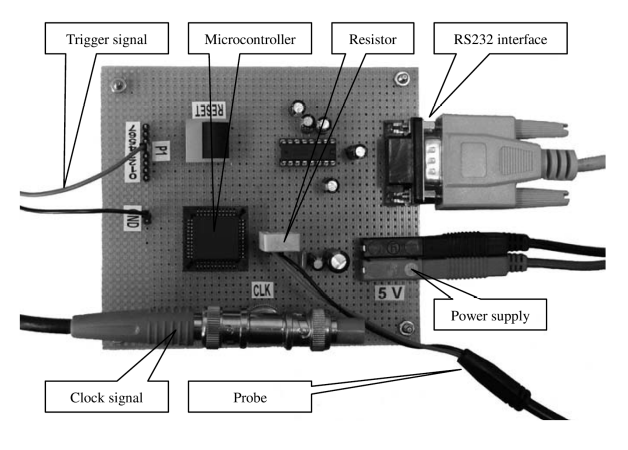
\includegraphics[scale=0.5]{images/Lecture_5/AES_setup.png}
\caption{AES Setup}\label{fig:AES Setup}
\end{figure}
 
While he's doing this operation it is going to consume different amount of power
and we would like to measure that. How do we going to measure them? We going to
connect to the microcontroller power supply. But were do we need to cut and
connect? The power is not going straight to the device it is going from this
white box (small resistor). How much power is going to go through the resistor?
Because he's small it's going to take very small power consumption. The voltage
drops across this device is going to be measured by this Probe, and I'm going to
measure the voltage over time. We know the voltage of the power supplies is 5
volt, so from this we can find out what is the current going through the
microcontroller and from the current we can find out what is the power
consumption. Do we need the code of the microcontroller? Yes. The only thing I
don't know is what? The secret, but I know everything else.
 
\section{Advanced Encryption Standard} 
 
What is the story about AES the encryption standard. 

In Death Valley Days encryption was in military standards it was considered like
a weapon you weren't supposed to have encryption, not by buy, export or sale.
but in the seventies the US government what is it might be a good idea to have
civilian encryption to protect civilian identities or health. they went to IBM
and ask them to write civilian encryption standard. IBM gave them an algorithm
called “Lucifer”, which was based on civilian Knowledge from the World War II,
the NSA I analyzed it and they say they don't actually like what you wrote and
change it. they changed the key change one of the internal tables and say this
was the standard. and the DES actually announced. the changes that NSA made was
making it difficult to implement it in software, and to make it Brute Force
about using the computing power that has the NSA but to protect it against some
kind of attack which was known to the NSA but not known in the Differential
cryptography ( not going to teach you).

The time passed and the computer got more and more powerful, there was something
called Deep cracking the electronic something, which was able to crack DES at
least. I'm not sure if they built it. This was too weak, so introduce something
called triple DES, it was twice as secure. Triple DES only used two keys, but
we're not going to study in this course. This wasn't so very efficient and it
was very slow. The US National standard unit, we want to create a new Cipher
which was at least as secure as Triple DES but much more efficient. Efficient on
software and hardware and slow computers. Anybody could submit candidates, the
winner of this competition was AES, which was a PhD work Raymond and Diamond.

It has some very good properties that we are going to talk about them.

\section{The Advanced Encryption Standard} 

How would you say AES is?, it is an operation which take 2 input, a kye and
plain text. And his output is ciphertext. How big is the plain text? 128 bit,
The input of the key is not always 16 bits, 16, 64,128 bits. Can go to AES 256
key. No one can break the 256 AES key. What if I wants to decrypt? AES can be a
reverse you can put the ciphertext the key and you get the plain text?. Can we
get the plain text and ciphertext so we can get the key? In theory we can do it
but the idea is that you cannot get the key. When you feed the key it has to
work a little bit, has to extend the key, create around key, this is done in
very secure facility. What if my input is more than 16 bytes? What if I need to
encrypt a file? I need to use a protocol and a mode, I can't just use AES, only
works on 16 bytes. If I have a larger data I need to use AES with a particular
way. Something called AES mode, the famous one called ECB, and CBC, the
fashionable called GCM. Not in this course and we don't really care, don't use
ECB. What if we want to encrypt just one byte? we need to do padding, there is a
trick and we need to do something. Let's talk about the design of a AES, it was
designed to resist all of source of the attacks, the attacks which were known in
the days of DES. And all sorts of attacks which were discovered using the
competition. AES was billed to be resistant for those attacks, script analysis
attack but no power analysis attack. They are basically expose the cipher if you
have enough plaintext and ciphertext.
 
AES won the competition because it was very fast or efficient. You have three
optimization goals when you're building a crypto implementation. You wanted to
be fast and to be able to encrypt as many bits. Maybe you want to encrypt all
the data in the router? You need to be fast and you want it to be power
efficient. You don't want to change your battery, and to be cheap so using as
little transistors as possible. Take at least area in the Silicon using a
smaller cheep. These three goals are conflict with each other, but if you want
go hardcore which AES is very very fast, if you want AES be larger. Particular
the AES submission the real-time paper head implementation of a s 8 bit 16 and
32 beats microcontroller which be being used till this day. One thing about a s
which is very nice is that if you remember the things that people were very very
suspicious about this AES that IBM present and a bunch of tables which values
that IBM didn't explain and then the NSA came back sage no so use these
different values and they also didn't explain why. I know that the NSA did
something good and what's nice about AES that he use a single lookup table for
all Xbox and this Lucas table is actually derived from mathematical relationship
some kind of a multiplication are over algebra field so it's not so hard there.
The design is so simple that you not be able to crypto even if you try. 

\section{AES Internals}
AES is an iterated cipher Which means eats has a very bASIC algorithm call
drafts and he does them all over and over again, AES has 10 Rounds, if you wants
to do it more complicated you as more and more rounds. How does as operated, you
begin with 16 bytes and put them in a cyber that's called stage register and
then you're on the round operations on these state bytes, every time you operate
operations the plaintext gets mixed with the key and every time you do it it
gets more and more. When you finish these 10 Rounds senior stage register you
have the ciphertext.

If you want to do it in a reverse you put the ciphertext and the stage register
and run the operation run after another and you get the plain text.

Each round consists of 4 basic operations, sub bytes, shift rows, mix columns,
and add around key.

Every operation was chosen by the creator Rijndael to achieve a different
objective. One of the objectives was to confusion, to make the aisle to put not
linear a dependent on the input, and I don't think they wanted to do what is
diffusion so all the output will depend on the input. We are mixing the
plaintext with the key with each one of the operation.

\subsection{SubBytes}
First one of the AES is sub bytes. Let's talk about this while thinking about
attacks. 

How do you implement on 8-bit microcontroller? The state is stored in memory so
I have 16 bytes of state, you read the first byte of state and the Sbox. Is a
table that stored in memory and the size of the table? 2**8. 

So I have this stage registered which is 16 bytes, and the sub box table 256
bytes. A full loop and I took the first byte, first you read it and then I
needed to read from the table who is the address that I just read and then I get
the value the Sbox, (we know inside the microcontroller) who does right
component units the value of the states and the value of the Xbox table, no XOR
them, no store that value in the stage register. Bridge from the state go to the
table, reading from the sub byte table and xor, and write.This operation is very
very leaky.

\begin{figure}[htp]
\centering
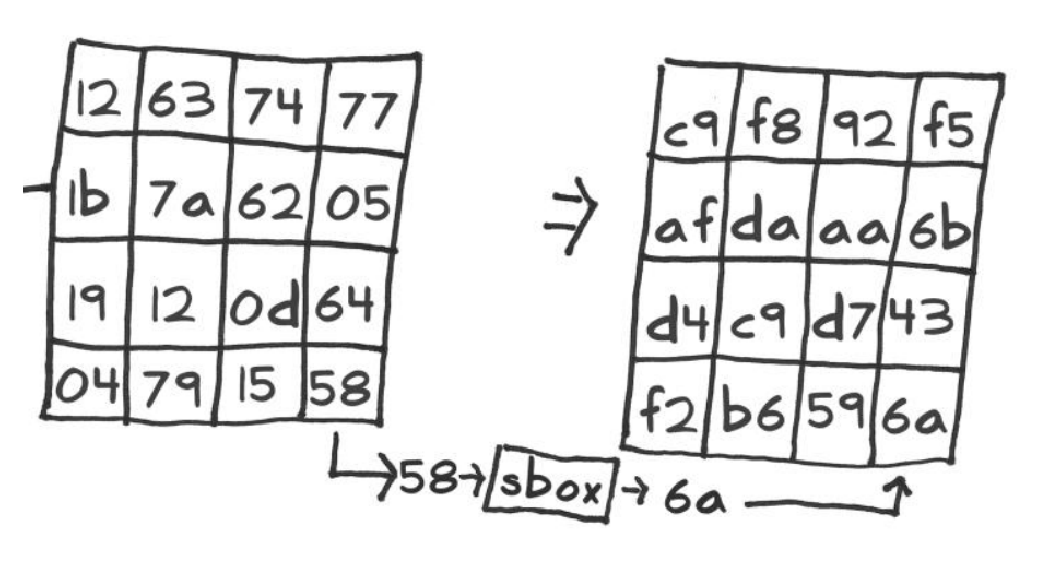
\includegraphics[scale=0.2]{images/Lecture_5/Subbytes.png}
\caption{SubBytes}\label{fig:SubBytes}
\end{figure}

\subsection{ShiftRows}

Then I need to do shift rows. The first row you don't need to do anything, the
other rows you need to shift them, how do you shift with 8-bit microcontroller?
using a temporary value, I read the state into the temporal value and I'm right
it into here. this is also a leaky operation, because I'm leaking all the bytes
in the state, well digging the Hemming Weights of the byte. another way to
implement it, just by imagination, it doesn't change the data so there are
actually operations that don't do shift row.

\begin{figure}[htp]
\centering
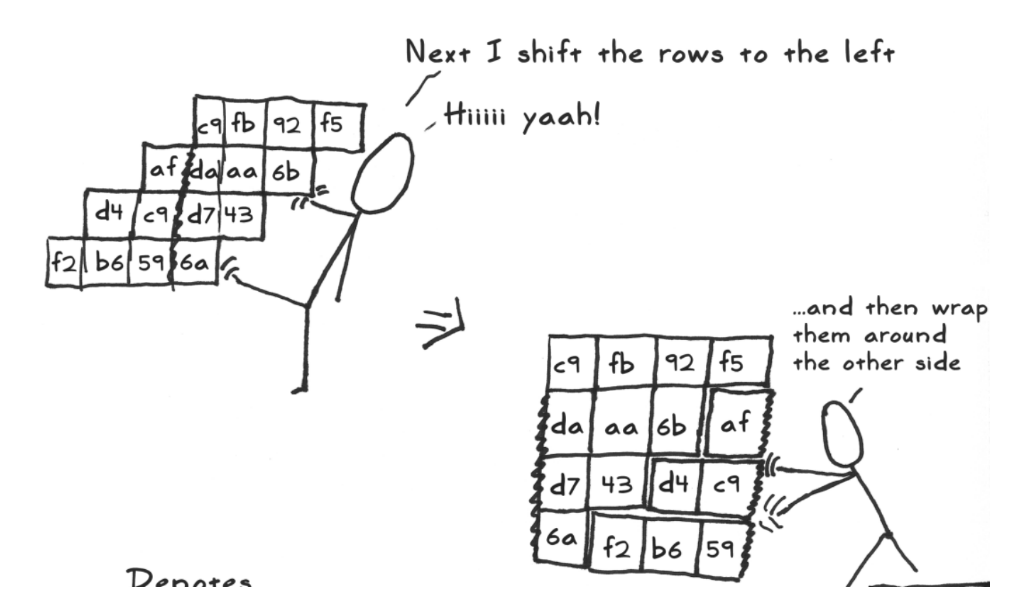
\includegraphics[scale=0.2]{images/Lecture_5/shiftrows.png}
\caption{ShiftRows}\label{fig:ShiftRows}
\end{figure}

\subsection{MixColumns}

Next operation mix columns, is the Matrix a complication, perform over algebra
algorithm, it's takes as input 32 bits columns and his output is 32 bytes value
what are all of the bytes in the output depend of input. How do you do it on a
microcontroller? One of the reasons that rhino run the competition that it was
very efficient way was doing mix column 8-bit microcontroller, using 13
operations which are shifts and exor. This is the most leaky part of AES this
mixed columns.

\begin{figure}[htp]
\centering
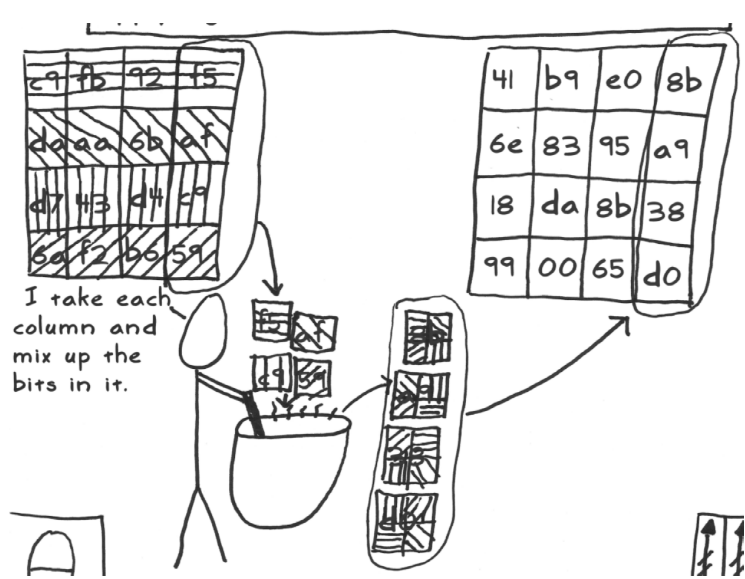
\includegraphics[scale=0.2]{images/Lecture_5/mixcolumns.png}
\caption{MixColumns}\label{fig:MixColumns}
\end{figure}

\subsection{AddRoundKey}

Then do a add round key, just xor, read xor write. This doesn't leak so much
because it is inside the ALU, but the reading and writing is the leaking here.
Each round of AES is 84 leaking actions. You take the key and you use the same
you used to do in creation but you don't have the plane text yet so you use sub
bytes or shift, then you end with the round, and this key expansion is very
sensitive for power analysis, you can really attack as very efficiently. We can
assume that this expansion is very secure.


\begin{figure}[htp]
\centering
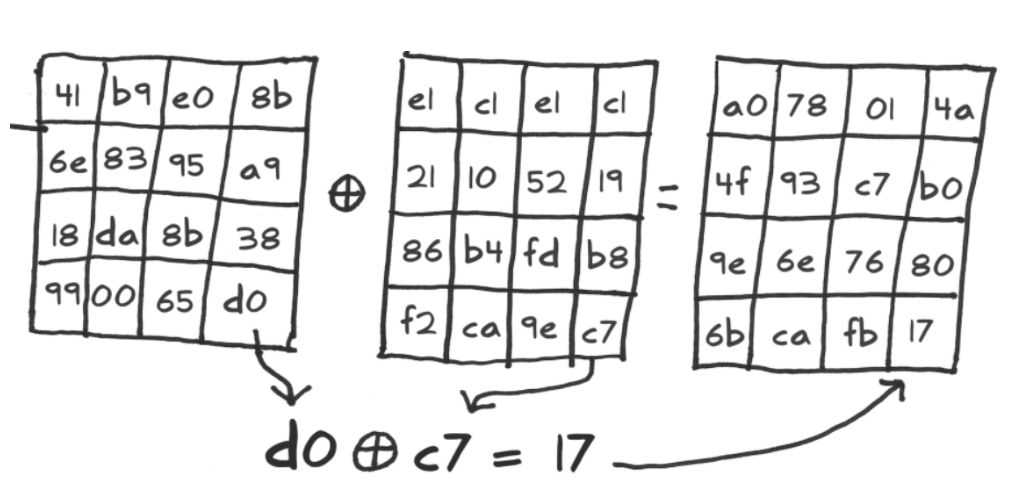
\includegraphics[scale=0.2]{images/Lecture_5/addkey.png}
\caption{AddKey}\label{fig:AddKey}
\end{figure}

\section{AES Power Analysis}
I told you about AES and what is our motivation and what is the structure, and I
want to spend the time that has left to show you a little about internal of AES
and very very very briefly talk about the reaction of doing simple power
analysis of AES. 

\begin{verbatim}
% Make sure the matlab AES scripts are in the path
addpath('matlab_aes_scripts');
%%
% Create two 128-bit plaintexts (exactly 16 byte)
plaintext_1 = uint8('Attack at 12:56!');
plaintext_2 = uint8('Attack at 12:57!');

% how many bits are different between the two?
disp(hamming_weight(bitxor(plaintext_1, plaintext_2)));
%%
% Create a key
key = uint8('1234512345123456');

ENCRYPT = 1;
DECRYPT = 0;
%%
% Encrypt the two plaintexts
ciphertext_1 = aes_crypt_8bit(plaintext_1, key, ENCRYPT); 
ciphertext_2 = aes_crypt_8bit(plaintext_2, key, ENCRYPT);
% even though the plaintexts were very similar...
disp([plaintext_1;plaintext_2]);
% ... the ciphertexts are very different
disp([ciphertext_1;ciphertext_2]);
%%
% how many bits are different between the two?
disp(hamming_weight(bitxor(ciphertext_1, ciphertext_2)));

%%
% Decrypt the two ciphertexts
decrypted_1 =  aes_crypt_8bit(ciphertext_1, key, DECRYPT); 
decrypted_2 =  aes_crypt_8bit(ciphertext_2, key, DECRYPT); 

% Did we get the plaintext again?
disp([plaintext_1;plaintext_2]);
disp([decrypted_1;decrypted_2]);
%%
% Look at the internals of AES now
[ciphertext_1, leak_1] = aes_crypt_8bit_and_leak(plaintext_1, key, ENCRYPT);
[ciphertext_2, leak_2] = aes_crypt_8bit_and_leak(plaintext_2, key, ENCRYPT);

% Show an image showing the two leaks side by size
subplot(1,3,1)
image(squeeze(leak_1));colormap(hsv(256));
subplot(1,3,3)
image(squeeze(leak_2));colormap(hsv(256)); 
figure(gcf)
%%
% Show the difference in the middle
subplot(1,3,2)
image(squeeze(bitxor(leak_1,leak_2)));colormap(hsv(256));
figure(gcf)
%%
% plot the HW of the difference
subplot(1,1,1)
bar(hamming_weight(bitxor(leak_1,leak_2)));
\end{verbatim}

What you see here is Matlab, I wrote this lab environment to do AES
implementations, There is code that dose AES, and there i  code that simulates
the power leakages of AES as it was implemented on 8-bit microcontroller, all of
the operations are 8 bits operations and each time operation happens I'm going
to leak it's Hamming Weight .Let's see what's going on. 

The first thing I'm going to do is to load some libraries and you can find them
in the middle, now going to create 216 bytes plain text. I am going to take
these string, to make it binary string Unit8, and I'm going to measure the
Hamming distance between these two strings. What is the time distance between
these two strings? One, the difference is 6 become 7. 110 - 111.

How do we do it, I have function called bitxor, and this is a vector of size
16,and then waiting Hamming weight. How many possibles Hamming weight are they
for 8 bits value? What can the Hamming weight to be? zero,1,2 … 8.So that
Hamming weight here is going to be one. now I'm going to set up a AES I am going
to choose a key.And now I'm going to encrypt AES, and then I'm going to use my
to plain text and the key. The Hamming distance between the two was one. What
will be the Hamming distance with the cipher text? Will it be one?no! what's
possible values it can be, between 0 to 128, because the output. Would you like
me to be 128? NO, I would like it to be 64. Why do I don't need it to be 100 or
2 or 3. Because that means that I don't have a very important property crypto
assistance in the Avalanche property means that each bit in each bit affect all
of the input. So if I change one bit in the input and I get only one change in
the output it means that I don't have the ability point. But if I change one bit
in the input and I get 100 bit change in the output what it is mean? It's means
that I don't have the average property and just to make things fun I'm flipping
all the bits. What I want the Hamming distance to be is around 64, It's that
exactly half of the bits changing. So you can see I'm doing the Hamming and
measuring and show the ciphertext, at the end I'm doing the Hamming weight.
 
These two strings are very very similar until the end, the 6 and 7 change. But
if you see the ciphertext you can see a lot of difference. And this humming
weight is 52. sometimes he's more sometimes is less than 64 but this is okay.
Now let's decrypt, How do I decrypt? I take my AES 8-bit function and I give it
decrypt. The ciphertext and the key. and see if the plain text into ciphertext
are the same. We can see that there are the same and so far so good. Now I want
to show you the internal structure of AES. to do that I have a function that's
called 8-bit and leak. Let's open the function. Here is the function. Let's go
over the structure

\begin{verbatim}
function [result state rkeys mixcolumn_leak]= 
aes_crypt_8bit_and_leak(input_data, secret_key, encrypt)

% performs AES-128 encryptions or decryptions like an 8-bit uC would do them
% and leaks internal state 
%
% DESCRIPTION:
%
% [result state rkeys mixcolumn_leak] = aes_crypt(input_data, secret_key, encrypt)
%
% This function performs an AES-128 encryption or decryption of the input
% data with the given secret key.
%
% PARAMETERS:
%
% - input_data:
%   A matrix of bytes, where each line consists of a 16 bytes (128 bit)
%   data input value of the AES-128 en/decryption.
% - secret_key:
%   A vector of 16 bytes that represents the secret key.
% - encrypt:
%   Paramter indicating whether an encryption or a decryption is performed
%   (1=encryption, 0=decryption).
%
% RETURNVALUES:
%
% - result:
%   A matrix of bytes of the same size as the byte matrix 'input_data'.
%   Each line of this matrix consists of 16 bytes that represent the
%   128-bit output of an AES-128 en/decryption of the corresponding line of
%   'input_data'.
% - state:
%   A matrix of byte of size |'input_data'| x 41, containins the state
%   progression of the encryption process.  
%   Legend of the state progression:
%   (P= plaintext, C=Ciphertext, K=after AddKey, B=after SubBytes, R=after
%   ShiftRows, M=after MixColumns)
%   P K BRMK BRMK BRMK BRMK BRMK BRMK BRMK BRMK BRMK BRK(=C)
% - mixcolumn_leak:
%   A matrix of size |'input_data'| x 9 x 4 x 9 (for encryption), or
%                    |'input_data'| x 9 x 4 x 18 (for decryption),
%       where mixcolumn_leak(line, subround, col, :) is the list of
%       intermediate valutes generated by the 8-bit MC operation on the
%       [col] columns of line [line] in the input data during
%       subroun [subround]
% EXAMPLE:
%
% result = aes_crypt([1:16; 17:32], 1:16, 1)


% AUTHORS: Stefan Mangard, Mario Kirschbaum, Yossi Oren
%
% CREATION_DATE: 31 July 2001
% LAST_REVISION: 28 October 2008

state = zeros([41 size(input_data)], 'uint8');
rkeys = zeros([10 16], 'uint8');
if (encrypt == 0) % decryption
    mixcolumn_leak = zeros([9 4 size(input_data,1) 18]);
else % encryption
    mixcolumn_leak = zeros([9 4 size(input_data,1) 9]);
end

for round = 1:10
    rkeys(round,:) = aes_round_key(secret_key,round);
end

% expand the keys

if encrypt == 0 %decryption
    state(41,:) = input_data;

    for i=10:-1:1
        if i ~= 10
            input_data = aes_add_round_key( aes_round_key(secret_key,i), input_data);
            state(3 + (i-1)*4 + 2,:) = input_data;

            [input_data leak] = aes_mix_columns_8bit_and_leak(input_data,0);
            mixcolumn_leak(i, :, :, :) = leak;
            state(3 + (i-1)*4 + 1,:) = input_data;
        else
            input_data = aes_add_round_key( aes_round_key(secret_key,i), input_data);
            state(3 + (i-1)*4 + 1,:) = input_data;
        end

        input_data = aes_shift_rows(input_data,0);
        state(3 + (i-1)*4,:) = input_data;

        input_data = uint8(aes_sbox(input_data,0));
        state(3 + (i-1)*4 - 1,:) = input_data;
    end

    input_data = aes_add_round_key(secret_key, input_data);
    state(1,:) = input_data;

else % encryption

    state(1,:) = input_data;
    input_data = aes_add_round_key(secret_key, input_data);
    state(2,:) = input_data;
    
    for i=1:10
        input_data = uint8(aes_sbox(input_data,1));
        state(3 + (i-1)*4,:) = input_data;

        input_data = aes_shift_rows(input_data,1);
        state(3 + (i-1)*4 + 1,:) = input_data;

        if i ~= 10
            [input_data leak] = aes_mix_columns_8bit_and_leak(input_data,1);
            mixcolumn_leak(i, :, :, :) = leak;
            state(3 + (i-1)*4 + 2,:) = input_data;

            input_data = aes_add_round_key( aes_round_key(secret_key,i), input_data);
            state(3 + (i-1)*4 + 3,:) = input_data;
        else
            input_data = aes_add_round_key( aes_round_key(secret_key,i), input_data);
            state(3 + (i-1)*4 + 2,:) = input_data;
        end
    end
            
end

result = input_data;

\end{verbatim}

First of all I expand the key, so I do the AES key expansion and I don't leak
the key expansion. This is the assumption. Let's disregarded that description
for a moment and this is the encryption. First of all I took the state and the
input data in the state, and then I do a add round key, then do SUB bytes, shift
rows, mix column. In the last round I done did you mixed columns, and every time
I do this I don't replace the state and I saved the state. at the end I output
the cipher text, but also the output to the state, so you can see the state is
always changing. Now let's see how does it looks, I'm going to run AES twice,
and then do some little figure.

\begin{figure}[!ht]
\centering
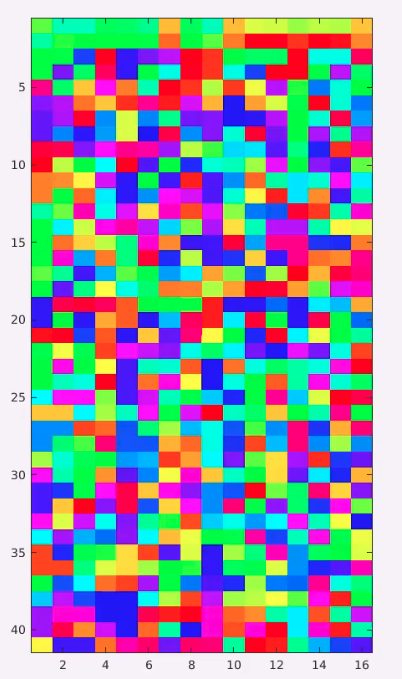
\includegraphics[scale=0.35]{images/Lecture_5/aes_mat_out.png}
\caption{Diagram}\label{fig:Diagram}
\end{figure}

The x-axis is the index of the byte in the state. I read the bytes not as a
matrix I read it as a row. So there are 16 bites in the state. and the y-axis is
the index of the rounds and round 40 is the final round ciphertext. So in
between there is the stages. You can see that in the beginning it is very very
similar.

If you go down it's become much different and in the bottom it's completely
different. This is very easy to analyze. And what we are going to do now show
the difference between state. What do you see in the middle is the Hemming
distance between the right and the left where red is is 0 and blue is 256.

In stage 0 what is the difference between two plain texts? 1 bit, you can see
one beat is changed to O. The first round is a add key, we xor the 15 bytes of
the key who is 16 bytes of the state, the key is the same in both sides, if the
Hamming distance between the two sides was one before I sold the key what is it
going to be after? 1. The differential doesn't change at all, I think a distance
of 1 and Ikes or a constant of both sides and The Outpost is still the same. so
in the first row I can't see differences. look wild sheep will do, one by the
interstate here, one byte is in the same place and one byte There and one byte
here. Now there are 4 bytes different between the states, but this bytes are all
of the column.What is the next operation? mixed columns. See what's mix column
did, mixed this change and now all of the bytes of the states are different.We
can't stop AES after 2 rounds, it still can break with crypto analysis, but you
can see that this is very nice.
 
I want to plug the Hamming weight of the distance, The x-axis here he's there
around, and the y-axis is the Hamming distance between the two stay. you can see
state with the one then one stays one, after sub byte becomes 4, Shift columns
doesn't change the 4, then mix columns make it grow a little bit. And then you
see the distance stays around 64 until the end of the encryption. I want to show
you how do we attack AES using simple power analysis.

There is a lot to talk about in very little time. in very very briefly I will
give you the ideal way did you it and then I'll show you how it's actually done.
I have connected a probe to my device, I have measured the power consumption
overtime. so now I have a vector of size that lets say a hundred thousand, and I
know that AES is there. Now I want to find the key out of my measurements from
my trace.

\begin{figure}[htp]
\centering
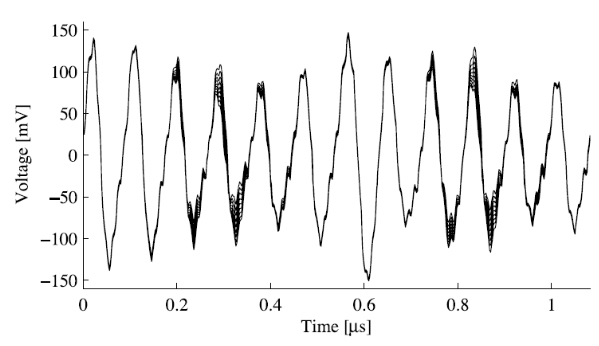
\includegraphics[scale=0.30]{images/Lecture_5/trace1.png}
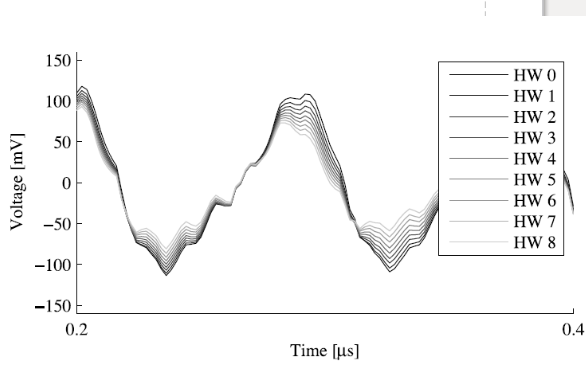
\includegraphics[scale=0.30]{images/Lecture_5/trace2.png}
\caption{Traces}\label{fig:traces}
\end{figure}

I have a trace, which was recorded in the same device we saw here. I have a
vector called 200 of traces of AES encryption, lets plot one of the traces. this
is actually only one of the rounds of AES. Here is a trace. This is very very
clean trace and I would like it to be in my lab.You can see some of them are
high and some of them are low, how do I find the key out of this? let's start
from the beginning then jump to the middle and the end I don't have time to
teach you. the best thing I can hope for is not to get the bytes of the key
because the bytes are not function of the bytes, what is the function of? The
Hamming weight. So the best hope is the get the Hamming weight, so are you home
we will get a vector like the state vector. is this enough to get the key? so
you have to believe me that's yes. how do you do it? You will use algebraic the
solver and you will have to read the paper. if you have the vector off all the
time in Hamming weight you can get the key. But how do I get the vector Hamming
weight from distance? Obviously somewhere in this trace, let's look at very very
leaky operation like sub bytes, or add around key; it read the states you leave
the key and xor them together and then you write the state again. Somewhere in
this vector there is a peak where we know that exactly in this moment there was
a read of the key. The key was read from memory and was travel in the data bus
in this exact peak. And how do I find this particular moment in time I will show
you in the next lecture.

So I need to write a function that gets an input about 20 points and what is its
out puts? the Hamming weight. maybe it will output of Hamming weight. how do I
do it? we need to write a decoder that's as single processing.

Here is a figure showing the move operation they did the same move operation in
the microcontroller over and over again this is the average of thousands of
measurements where are they moving 0 or 1, until moving 255 ff. Can anybody, you
see how Hamming Weight zero have big change, why Hamming weight 0 is more power
consumption of Hamming weight 8? Between moves it settings old ones, so moving
to zero take more effort from changing.
 
Here is like a longer trace, let's assume I hate this data how do I build the
decoder. I want the function that can take an array of values and output Hamming
weight. Let's start simple, what if I had just one point? I have an input and
function that gets one point and give me the Hamming weight of this point. I can
calculate the mean each one, the mean for 0 the mean for 1, for 2. if I get it
right what we will do, so do you like a nearest neighbor. if I know that the
mean of 4 Hamming weight for is 7 and the mean of Hamming weight five is 8 and I
got 7.9, what am I going to chose 4 or 5? 5.nearest neighbor.

This is a nice idea, but I have to give them a little extra dangerous. the
problem is here that's the Hamming weight are not identically distributed. how
many possible values of bytes I get? 256. how many bytes are there with Hamming
weight zero? 1. how many bytes Hamming weight 8? 1. how many Hamming weight 1?
8. Hamming weight of 1 is 8 times more likely than Hamming weight of 0. So why
do we need to do?we need to do Bayes. The idea is are you going to favor the
output more likely. I will found out what are the odds that its five, 6?, 7?
then look on my decoder and then I'm going to look and give a bonus for more
common Hamming weight. The idea is I need to learn How likely bytes based on the
trace decoding and then I'm going to go and look at the distribution of this and
then multiply The probability I got. this is for one point. I calculated the
odds and then I multiply the probability. what if I have more than one point?
watch we actually wants to do here he's actually called multivariate normal
distribution. each one of these points, let's say four points, the dimension,
and I have a like a cloud In this distribution space, how do you do this? that
is the very very fundamental paper called “template power analysis attack” which
explain this.

So if you want to do a simple power analysis on AES the steps you do first of
all you profiled the device, you understand where all this stuff is happening,
you need to build Template that will help you to recognize different Hamming
Weight, then you're play the same place in the trace and you get guesses for
Hamming weight for each States and you hope you get the right guesses, and then
you take this Hamming weight and you take a few equation solver we'll take the
Hamming weight and output the key, or something that we don't know? I don't know
because noise. If we can correlate the Hamming weight to wrong then the equation
solver will fail. what can we do in this case? We try again.

\newpage
\section{Template Attacks} 
\subsection{Introduction}
    Devices performing cryptographic operations can be analyzed by various
    means. Traditional cryptanalysis looks at the relations between input and
    output data and the used keys. However, even if the implemented algorithms
    are secure from a cryptanalysis point of view, side-channel attacks pose a
    serious threat. Sidechannel attacks are a subgroup of implementation
    attacks. Examples thereof are timing attacks, power attacks like DPA or SPA.
    Traditional DPA style attacks assume the following threat model: The secret
    key stored in the device is used to perform some cryptographic operations.
    The attacker monitors these operations using captured side-channel
    information like power consumption or electromagnetic emanation. The attack
    is successful if the used secret key can be reconstructed after a certain
    number of operations.\textbf{If the number of operations is limited by the
    protocol used to initiate} these operations, the attacker has an upper bound
    on the number of operations he can observe. If the operation, which leaks
    usable side-channel information, is executed just once, the threat model is
    different: The attacker has to reconstruct the secret key using a single
    trace of side-channel information. Besides protocol limitations, ephemeral
    keys can be the reason for such a constraint. Techniques like SPA are a
    general way to tackle this problem. These techniques useeasily
    distinguishable features of operations like double and add, or add and
    multiply, to infer key-bits. The majority of the available literature deals
    with these two types of scenarios. \textbf{If the observed signal-to-noise
    ratio is not high enough, or the implementation is done in a way that
    ensures the used operations being independent of the key(i. e. no
    key-dependent jumps), SPA style attacks are not possible anymore.} The
    attacker has to think of other ways to get hold of the secret key: One way
    to do this is to use a similar device and build a model of it. Using this
    model, an attacker might now be able to recover the secret key.
    
\subsection{Algorithm}
    Template attacks are a powerful type of side-channel attack. These attacks
    are a subset of profiling attacks, where an attacker creates a ``profile" of
    a sensitive device and applies this profile to quickly find a victim's
    secret key.
    
    Template attacks require more setup than CPA attacks. To perform a template
    attack, the attacker must have access to another copy of the protected
    device that they can fully control. Then, they must perform a great deal of
    pre-processing to create the template - in practice, this may take dozens of
    thousands of power traces. However, the advantages are that template attacks
    require a very small number of traces from the victim to complete the
    attack. With enough pre-processing, \textbf{the key may be able to be
    recovered from just a single trace} .
    
    
    There are four steps to a template attack:
    \begin{itemize}
      \item Using a copy of the protected device, record a large number of power
      traces using many different inputs (plaintexts and keys). Ensure that
      enough traces are recorded to give us information about each subkey value.
      \item Create a template of the device's operation. This template notes a
      few ``points of interest" in the power traces and a multivariate
      distribution of the power traces at each point.
      \item the victim device, record a small number of power traces. Use
      multiple plaintexts. (We have no control over the secret key, which is
      fixed.)
      \item Apply the template to the attack traces. For each subkey, track
      which value is most likely to be the correct subkey. Continue until the
      key has been recovered.
    \end{itemize}
    
    \subsection{Signals, Noise, and Statistics}
    Before looking at the details of the template attack, it is important to
    understand the statistics concepts that are involved. A template is
    effectively a multivariate distribution that describes several key samples
    in the power traces. This section will describe what a multivariate
    distribution is and how it can be used in this context. Noise
    Distributions\\
    Electrical signals are inherently noisy. Any time we take a voltage
    measurement, we don't expect to see a perfect, constant level. For example,
    if we attached a multi-meter to a 5 V source and took 4 measurements, we
    might expect to see a data set like (4.95, 5.01, 5.06, 4.98). One way of
    modelling this voltage source is: $\mathbf{X} = \mathbf{X} + \mathbf{N}$
    where $\mathbf{X}$ is the noise-free level and $\mathbf{N}$ is the
    additional noise. In our example, $\mathbf{X}$ would be exactly 5 V. Then, N
    is a random variable: every time we take a measurement, we can expect to see
    a different value. Note that $\mathbf{X}$ and $\mathbf{N}$ are bolded to
    show that they are random variables. A simple model for these random
    variables uses a Gaussian distribution (read: a bell curve). The probability
    density function (PDF) of a Gaussian distribution is f(x) = $
    \frac{1}{\sigma \sqrt{2\pi}} e^{-(x - \mu)^2 / 2\sigma^2}$ where
    $\displaystyle \mu$  is the mean and  $ \sigma$ is the standard deviation.
    For instance, our voltage source might have a mean of 5 and a standard
    deviation of 0.5, making the PDF look like:\\
    \begin{minipage}{\linewidth}
    \centering
    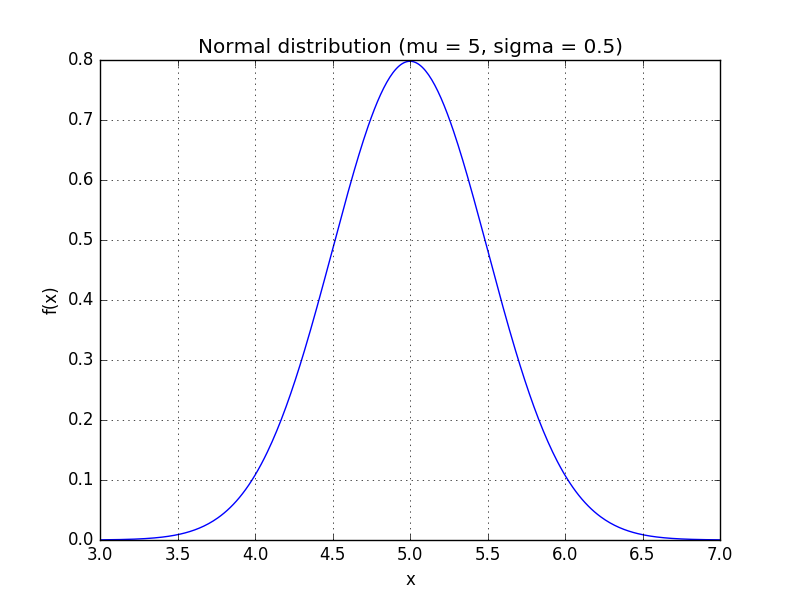
\includegraphics[width=8cm]{images/Lecture_5/Normal-Dist.png}
    \end{minipage}
    We can use the PDF to calculate how likely a certain measurement is. Using
    this distribution, $f(5.1) \approx 0.7821$ $f(7.0) \approx 0.0003$ so we're
    very unlikely to see a reading of 7 V. We'll use this to our advantage in
    this attack: if f(x) is very small for one of our subkey guesses, it's
    probably a wrong guess.\\
    Multivariate Statistics The 1-variable Gaussian distribution works well for
    one measurement. What if we're working with more than one random variable?
    Suppose we're measuring two voltages that have some amount of noise on them.
    We'll call them $\mathbf{X}$ and $\mathbf{Y}$. As a first attempt, we could
    write down a model for $\mathbf{X}$ using a normal distribution and a
    separate model for $\mathbf{Y}$ using a different distribution. However,
    this might not always make sense. If we write two separate distributions,
    what we're saying is that the two variables are independent: when
    $\mathbf{X}$ goes up, there's no guarantee that $\mathbf{Y}$ will follow it.
    Multivariate distributions let us model multiple random variables that may
    or may not be correlated. In a multivariate distribution, instead of writing
    down a single variance $\sigma$, we keep track of a whole matrix of
    covariances. For example, to model three random variables ($\mathbf{X},
    \mathbf{Y}, \mathbf{Z}$), this matrix would be\\
    
    \begin{minipage}{\linewidth}
      \centering
      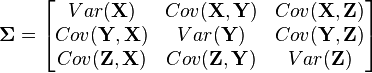
\includegraphics[scale=0.6]{images/Lecture_5/cov.png}
      \end{minipage}\\
      
      
    Also, note that this distribution needs to have a mean for each random
    variable:\\
    
       \begin{minipage}{\linewidth}
      \centering
      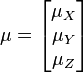
\includegraphics[scale=0.7]{images/Lecture_5/mu.png}
      \end{minipage}\\
      
      
    The PDF of this distribution is more complicated: The equation for k random
    variables is:\\
    
     \begin{minipage}{\linewidth}
      \centering
      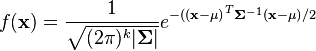
\includegraphics[scale=0.7]{images/Lecture_5/dist.png}
      \end{minipage}

\subsection{Creating the Template}
    A template is a set of probability distributions that describe what the
    power traces look like for many different keys. Effectively, a template
    says: ``If you're going to use key k, your power trace will look like the
    distribution $f_k(\mathbf{x})$"\\
    . We can use this information to find subtle differences between power
    traces and to make very good key guesses for a single power trace.\\
    \\
    \textbf{Number of Traces}\\
    One of the downsides of template attacks is that they require a great number
    of traces to be preprocessed before the attack can begin. This is mainly for
    statistical reasons. In order to come up with a good distribution to model
    the power traces for every key, we need a large number of traces for every
    key. For example, if we're going to attack a single subkey of AES-128, then
    we need to create 256 power consumption models (one for every number from 0
    to 255). In order to get enough data to make good models, we need tens of
    thousands of traces.
    
    Note that we don't have to model every single key. One good alternative is
    to model a sensitive part of the algorithm, like the substitution box in
    AES. We can get away with a much smaller number of traces here; if we make a
    model for every possible Hamming weight, then we would end up with 9 models,
    which is an order of magnitude smaller. However, then we can't recover the
    key from a single attack trace - we need more information to recover the
    secret key.\\
    \\
    \textbf{Points of Interest}\\
    Our goal is to create a multivariate probability describing the power traces
    for every possible key. If we modeled the entire power trace this way (with,
    say, 3000 samples), then we would need a 3000-dimension distribution. This
    is insane, so we'll find an alternative.
    
    Thankfully, not every point on the power trace is important to us. There are
    two main reasons for this:
    \begin{itemize}
      \item We might be taking more than one sample per clock cycle.  There's no
      real reason to use all of these samples - we can get just as much
      information from a single sample at the right time.
      \item Our choice of key doesn't affect the entire power trace. It's likely
      that the subkeys only influence the power consumption at a few critical
      times. If we can pick these important times, then we can ignore most of
      the samples. 
    \end{itemize}
    
    These two points mean that we can usually live with a handful (3-5) of
    points of interest. If we can pick out good points and write down a model
    using these samples, then we can use a 3D or 5D distribution - a great
    improvement over the original 3000D model.
   \subsection{Analyzing the Data}
    Suppose that we've picked I points of interest, which are at samples $s_i (0
    \le i < I)$. Then, our goal is to find a mean and covariance matrix for
    every operation (every choice of subkey or intermediate Hamming weight).
    Let's say that there are K of these operations (maybe 256 subkeys or 9
    possible Hamming weights).
    
    For now, we'll look at a single operation k $(0 \le k < K)$. The steps are:
    \begin{itemize}
      \item Find every power trace t that falls under the category of
      ``operation k". (ex: find every power trace where we used a subkey of
      0x01.) We'll say that there are $T_k$ of these, so $t_{j, s_i}$ means the
      value at trace j and POI i.
      \item Find the average power $\mu_i$ at every point of interest. This
      calculation will look like:
      \begin{figure}[htp]
      \centering
      \includegraphics[scale=0.7]{images/Lecture_5/pc1.png}
      \end{figure}
       
      \item Find the variance $v_i$ of the power at each point of interest. One
      way of calculating this is:
      \begin{figure}[htp]
      \centering
      \includegraphics[scale=0.7]{images/Lecture_5/pic2.png}
      \end{figure}
    
      \item Find the covariance $c_{i, i^*}$ between the power at every pair of
      POIs $(i and i^*)$. One way of calculating this is:
      \begin{figure}[htp]
      \centering
      \includegraphics[scale=0.7]{images/Lecture_5/pic3.png}
      \end{figure}
      \item Put together the mean and covariance matrices as:
    
      \begin{minipage}{\linewidth}
      \centering
      \includegraphics[scale=0.7]{images/Lecture_5/pic5.png}
      \end{minipage}
      \begin{minipage}{\linewidth}
      \centering
      \includegraphics[scale=0.7]{images/Lecture_5/pic4.png}
      \end{minipage}
      
    \end{itemize}
    
    These steps must be done for every operation k. At the end of this
    preprocessing, we'll have K mean and covariance matrices, modelling each of
    the K different operations that the target can do.

    \subsection{Attack Time}
    With a template in hand, we can finish our attack. For the attack, we need a
    smaller number of traces - we'll say that we have A traces. The sample
    values will be labeled $a_{j, s_i} (1 \le j \le A)$. First, let's apply the
    template to a single trace. Our job is to decide how likely all of our key
    guesses are. We need to do the following:
    \begin{itemize}
      \item Put our trace values at the POIs into a vector. This vector will be:
      
       \begin{minipage}{\linewidth}
      \centering
      \includegraphics[scale=0.7]{images/Lecture_5/pic6.png}
      \end{minipage}
       
      \item Calculate the PDF for every key guess and save these for later. This
      might look like:
      \begin{minipage}{0cm}
      \centering
      \includegraphics[scale=0.7]{images/Lecture_5/pic7.png}
      \end{minipage}
      \item Repeat these two steps for all of the attack traces
    \end{itemize}
    This process gives us an array of $p_{k, j}$, which says: ``Looking at trace
    j, how likely is it that key k is the correct one?"\\
    \textbf{Combining the Results}\\
    The very last step is to combine our $p_{k, j}$ values to decide which key
    is the best fit. The easiest way to do this is to combine them as:
    
    \begin{figure}[htp]
        \centering
        \includegraphics[scale=0.7]{images/Lecture_5/pic8.png}
       \end{figure}
    
    \subsection{practical template attacks}
    In this section we will show a differant ways to select the most important
    point of a power trace, that will lead us to improved computation time and
    make template attack more practical.\\
    \\
    \textbf{sum of difference}
       \begin{itemize}
          \item For every operation k and every sample i, find the average power
          $M_{k, i}$. For instance, if there are $T_k$ traces where we performed
          operation k, then this average is\\
              \begin{minipage}{\linewidth}
              \centering
              \includegraphics[scale=0.7]{images/Lecture_5/pic9.png}
              \end{minipage}
           
          \item After finding all of the means, calculate all of their absolute
          pairwise differences. Add these up. This will give one ``trace" which
          has peaks where the samples are usually different. The calculation
          looks like\\
          \\
              \begin{minipage}{\linewidth}
              \centering
              \includegraphics[scale=0.7]{images/Lecture_5/pic10.png}
              \end{minipage}
       \end{itemize}
        An example of this sum of differences is:\\
              \begin{minipage}{\linewidth}
              \centering
              \includegraphics[scale=0.7]{images/Lecture_5/pic11.png}
              \end{minipage}
        \\

\textbf{Preprocessing}\\
    In practical side-channel analysis, the raw input data is often
    preprocessed. Sometimes this is just due to simplicity or efficiency
    reasons, e. g. summarizing sampled points. There are however cases where the
    preprocessing step heavily affects the results. Even if no thinkable
    transformation can add additional information to a signal, information
    extraction procedures do improve. The template attack under consideration is
    such a case and a lucrative preprocessing transformation is described
    subsequently. It turns out that the transformation of the input traces from
    the time domain into the frequency domain is such a lucrative
    transformation. In our practical work, an FFT algorithm was used to
    accomplish this transformation (a fast algorithm to calculate the discrete
    Fourier transform, for background information refer to [BP85]). In order to
    show the impact of this preprocessing step a number of experiments were
    carried out. First some characteristic differences between time domain
    analysis and frequency domain analysis are illustrated. Afterwards, to
    highlight the influence of the number of selected points on the
    classification performance in the frequency domain, a number of experiments
    were carried out. After preprocessing, the resulting traces can be used to
    perform a template attack in exact the same way as without preprocessing.
    There is however a difference in the number of points to consider. Figure 6
    shows the classifications results as a function of the number of selected
    points after preprocessing. The considered numbers of points are ranging
    between 1 and 40. Additionally three different minimum distances where
    chosen. Results show that much less points are sufficient in comparison to a
    template attack without the preprocessing step. At the price of performing
    an FFT on every input trace (those used to build up the templates as well as
    those to classify) we get a major advantage\\


\textbf{Amplified Template Attack}

    Even if the aim of a template attack is to recover the secret key using a
    single trace, in many real world settings implementations allow for several
    iterations of the same operation with the same secret key. The application
    of template attacks is not restricted to stream ciphers like RC4 and can be
    applied to block ciphers as well. Since every symmetric cipher contains some
    sort of key scheduling mechanism which processes the secret key, this
    generalization is possible. Smartcards often use block ciphers for
    encryption or authentication, hence let us consider the following example: A
    malicious petrol station tenant, named Eve, is using a modified smartcard
    based payment terminal. Everytime a customer uses this terminal, Eve
    captures one trace of side-channel information. This single trace could
    already be used by Eve to carry out a template attack. However, some
    customers are coming again and Eve gets hold of another trace. The template
    attack can easily be extended to take advantage of such situations, e.g. by
    adding up noise-probabilities p(Ni) of every captured trace and applying the
    maximum-likelihood approach on these sums. As a consequence, the power of
    the attacker is amplified. Using this approach, if n is the number of
    iterations, the error probability of template classification is reduced by
    the factor √n. 


\chapter{Introduction to micro-architectural attacks}
\label{chap:c7_cacheattacks}

Clementine Maurice, CNRS, IRISA\\
April 30, 2019 — Ben Gurion University, Israel

\section{Background \& Primitives} %arbel
\label{sec:BackgroundnPrimitives}

Micro-architectural side-channel attacks refers to a side-channel attack that
exploit information leakage from the hardware infrastructure itself. The attacks
can be found in a large scope on devices - servers, workstations, laptops,
smart-phones, etc.

Normally, we assume a safe software infrastructure. Meaning that no software
bugs, such as buffer overflow, is present. Nevertheless, such assumption does
not imply safe execution, due to the fact that the information leaks because of
the implementation, which is often driven by complex optimizations and design.
Such leakages are not considered as 'mistakes' or 'bugs', but rather a trade-off
decision between optimizing some aspects of the execution and potential
information leakage.    

Potential outcomes of such attacks as described can be crypto primitives, which
is common with other side-channel attacks, but also other sensitive information
such as keystrokes and mouse movements.  

In terms of sources of leakage, we saw in previous chapters sources such as
power consumption or electromagnetic leaks. However such sources are harder to
come across by an attacker because they require physical proximity and access to
the device, which is more typically to embedded devices. In our case we are only
require that the attacker have somewhat remote access to the device, meaning
that the attacker can run code on the hardware infrastructure of the machine.
Such scenarios can be found in cloud providers renting computational resources
to a costumer, Java-Script code running in a browser and others.

\subsection{Example: Cache attack on RSA Square-and-Multiply Exponentiation}
\label{subsec:CacheattackonRSA}

\begin{algorithm}
    \SetKwInOut{Input}{Input} \SetKwInOut{Output}{Output} \Input{base $b$,
    exponent $e$, modulus $n$} \Output{$b^e$ mod $n$} $X \leftarrow 1$ \For{$i
    \leftarrow bitlen(e)$ \textbf{downto} $0$} {$X \leftarrow multiply(X,X)$
    \If{$e_i = 1$} {$X \leftarrow multiply(X,b)$}} \textbf{return} X
    \caption{Square-and-multiply exponentiation}
    \label{algo:SaM}
\end{algorithm}

Consider the binary exponentiation algorithm presented in Algorithm
\ref{algo:SaM}. Notice that the execution flow of the algorithm relies heavily
on the value of the bit $e_i$ of the private key. Now consider a scenario in
which an attacker has information on the changes regarding the buffer holding
the multiplier $b$. Such information can be considered as a query to the buffer
and receiving as a result the latency of the query. If the buffer is in use, the
query will be longer then if the buffer is unused.

\begin{figure}
    \centering
    \includegraphics[width=\textwidth]{images/chapter_6/PPSM.PNG}
    \caption{Querying the buffer holding the multiplier $b$. The y axis is a latency scale, and the x axis represent the query index. The dotted plot is a scatter plot while the solid line is the normalized moving average.}
    \label{fig:PPSQ}
\end{figure}

In \Cref{fig:PPSQ} the resulting graph of the querying can be seen, in which the
actual bits of the exponent can be clearly detected.

\subsection{Attack Model}
\label{subsec:attackmodel}
We assume that the attacker has no physical access to the device. Moreover, the
attacker can only execute unprivileged code on the same machine as victim. Such
scenarios in which this happens can be found, for example, when the victim
install some malicious program on his machine/smartphone. Another examples can
be found in could computing where an attacker has a victual machine on the same
physical machine as the victim, or in a web environment in which the attacker
runs unprivileged JavaScript code.

In the scope of this chapter we will focus on shared hardware in the form of
data/instruction cache. While other shared hardware components can also include
the DRAM and the memory bus (memory shared hardware) or the branch prediction
unit and the arithmetic logic unit (CPU shared hardware), they are not in the
scope of this chapter.

\subsection{Today's CPU Complexity}
\label{subsec:todaycpucomplex}
From 2012 onwards Intel has released a new family of microprocessors every year.
Each comes with its own new microarchitectural schemes with new Characteristics.
To gain performance upgrade in each new installment, that has on average 5\%
increase in performance depending on the feature, very small optimizations, such
as caches and branch prediction units are added. Such optimizations are the main
reason for a side-channel information leakage to exist. Unfortunately, said
optimization often come with no documentation since this is Intel intellectual
property. Such lack in documentation makes it harder for an attacker to perform
said side-channel attacks.

To emphasize today's CPU complexity, it is said that ``Intel x86 documentation
has more pages than the 6502 has transistors"~\cite{IntMan}, with 6502 being a
reference to a 8-bit microprocessor, used in Apple II, Commodore 64, Atari 800
and more. It had, in the year 1975, roughly 3510 transistors, while the Intel
Software Developer's Manuals is 4844 pages (may. 2018). In a more advance
microprocessor, such as the 22-core Intel Xeon Broadwell-E5, more than 7 billion
transistors can be found. 

\subsection{Background on Caches}
\label{subsec:backgroundoncaches}
In designing a cache side-channel attack, a proper understanding of how caches
work, in great detail, is required. First, we need to acknowledge that the
requirements for an 'ideal memory' oppose each other. Such requirements are zero
latency, infinite capacity, zero cost and infinite bandwidth. The trade-offs are
interconnect: \textbf{Bigger is Slower} - Bigger memory often comes with higher
latency, due to the fact the it would take longer to determine the location to
retrieve.  \textbf{Faster is Expensive} - A reduction in latency often means
that a more expensive technology a needed. For example, SRAM is faster than
DRAM, which in turn is faster than Disk memory. However, their cost ratio is the
other way around. \textbf{Bandwidth is Expensive} - A wider bandwidth needs to
come with additional banks, ports, higher frequency or faster technology. 

In our need to understand the use of caches, we need to examine the different
memory technologies and why they are used the way they do. \textbf{DRAM} -
Dynamic Random Access Memory is the technology that is often used as the main
memory (or RAM), while \textbf{SRAM} - Static Random Access Memory is the
technology used in caches. The DRAM latency is higher than the SRAM latency, but
is cheaper to make. The main difference in cost arises from the fact that DRAM
consist only of one transistor and one capacitor per cell, while the SRAM
consist of six transistors per cell. Said difference also mean that DRAM is more
dense. Finally, the DRAM cell layout and technology requires to periodically
refresh each cell.

Since having Both a large and fast, single level of memory is unlikely, CPU's
today are made with multiple levels of storage. The main idea is that
progressively bigger and slower storage units are located in higher levels of
memory, which are farther from the processor. The motivation for such design is
to ensure that most of the data the processor needs is kept in the closer and
faster levels.

\begin{figure}
    \centering
    \includegraphics[width=\textwidth]{images/chapter_6/MemHier.PNG}
    \caption{Memory Hierarchy of a common CPU.}
    \label{fig:MemHier}
\end{figure}

The memory hierarchy can be seen in \Cref{fig:MemHier}, where data can reside
in, at a given point in time, in the following storage units - in CPU registers,
the different levels of the CPU cache, main memory or disk memory. 

\subsection{Caching Basics}
\label{subsec:cachingbasics}
The two main idea of caching is to exploit temporal and spatial locality.
\textbf{Temporal Locality} is the notion that a program tends to reference the
same memory location many times within a small window of time (for example,
loops). The anticipation of such thinking is that recently accessed data will be
accessed again soon. Therefor, a good strategy will be to store recently
accessed data in automatically managed fast memory. \textbf{Spatial Locality} is
the notion that a program tends to reference a cluster of memory locations at a
time (for example, sequential instruction access or array traversal). The
anticipation will be that surrounding of some accessed data will be accessed
soon. A good strategy will consider storing addresses adjacent to the recently
accessed one in an automatically managed fast memory. In detail, we want to
logically divide memory into equal size blocks (lines) and fetch to cache the
accessed block in its entirety.   

Moreover, there are two approaches to the management scheme, manual and
automatic. \textbf{Manual Management} means that the programmer manages data
movement across levels, which is not scalable for substantial programs. However,
it is sometimes used in some embedded systems. \textbf{Automatic management}
refer to a scheme in which the hardware itself manages data movement across the
different levels in a way that is transparent to the programmer. Meaning that
the average programmer does not need to know anything related to the memory
hierarchy levels to write a program. On the down side, which begs the question
on how to write a fast program if the management is automatic, in addition to
what kind of side-channels could arise from such scenario.

The basic unit of storage in the cache is called a block or a line. The main
memory is logically divided into cache blocks that map to locations in the
cache. And when data is referenced, two outcomes can come of such action - a
cache hit or a cache miss. A \textbf{Cache Hit} occurs when a line is referenced
and is in the cache. The cached data will be retrieved instead of accessing main
memory.  A \textbf{Cache Miss} occurs when a line is referenced and is not in
the cache. The data will be fetched from main memory, passing though the cache,
possibly eviction other data to ensure enough storage.

When designing a cache, we are faced with a number of design decisions to
handle. \textbf{Placement}  - Essentially the place in which we will place or
find a block in the cache. \textbf{Replacement} - We need often to remove data
from the cache to make room for newer data. Which begs the question of what data
to evict. \textbf{Granularity of Management} - The basic units of storage in
different levels. Do we store the same amount of blocks across different levels
or do we uniformly store the same size of blocks. \textbf{Write Policy} - When a
write is being made, we need to decide whether to preform the write operation in
all levels or passing the write data to a lower level only upon eviction from
that level. \textbf{Instruction/Data} - When a program is executing, the
instructions that are in need to be executed are required to be fetched from
memory as well. The designer needs to decide whether to treat instruction and
data memory as two separate  types or as one of the same.


\subsection{Set-Associative Caches}
\label{subsec:setassoccaches}

We will be focusing on a cache design that is often used in today's CPUs, which
is set-associative caches. Which means that the cache will be logically divided
into \textbf{Cache Sets}, which will be divided into \textbf{Cache Ways}. Each
way will store a cache line worth of data. The division of the memory into
different cache sets will be a direct mapping from the memory address. Namely,
each address will be associated with a cache set according to a group of bits in
the address which will represent the cache set index. The specific way in which
the line will is to be fetch will be determine according to the cache
replacement policy, since the cache set is expected to be full.  An abstraction
can be seen in \Cref{fig:SetWay}


\begin{figure}
    \centering
    \includegraphics[width=\textwidth]{images/chapter_6/SetWay.PNG}
    \caption{Set-Associative Cache - The set index of a line derives from the set index bits of the address. The cache way is determine according to the cache replacement policy.}
    \label{fig:SetWay}
\end{figure}

Consider the following example: The cache has 8B cache lines, 16 cache sets each
consisting of 2 ways. We can compute the set index of the address
$(1011111110)_b$ by only looking at bits $b_3, b_4, b_5, b_6$, since we have 16
cache sets (4 bits) and 8 different cache line offset (bits $b_0, b_1, b_2$).
Hence the cache set will be $(1111)_b$. We can also compute the size of the
whole cache by multiplying the cache dimensions $8 \times 16 \times 2 = 256 $B.

\subsection{Virtual Addresses or Physical Addresses}
\label{subsec:addrorphysicaladdr}
Since we need the bits of address to determine its cache set, we are face with a
problem due to the fact that programs running are only aware to the virtual
addresses while the hardware side is aware to the physical addresses. The
translation between virtual addresses and physical addresses is the
responsibility of the MMU (Memory Management Unit).

There are four major ways of implementing such cache mapping according to the
addresses. \textbf{VIVT} - Virtually-Indexed, virtually-Tagged. Meaning that
there is no need to translate the addresses in order to know the mapping of the
addresses into the cache, which is faster. On the other hand, such
implementation causes aliasing issues as same virtual address maps to several
different physical addresses. This aliasing is due to the tag not being unique,
and will force a flush action to the entire cache on context swiching.
\textbf{VIPT} - Virtually-Indexed, Physically-Tagged. Meaning that there will be
a need for TLB translation for the tag, but can be looked up in parallel. Such
mapping can be quiet fast. Moreover, if the set index bits are derived from the
page offset, there is no aliasing, but the cache size is limited to the page
size multiply by the number of cache sets. VIPT is used in Intel's L1 caches,
with the default page size being 4K and each cache line is 64B, resulting in no
larger than $2^6 = 64$ sets. \textbf{PIPT} - Physically-Indexed,
Physically-Tagged. Meaning that the translation between virtual and physical
addresses will have to be preformed, taking up time. On the other hand, no
aliasing issues occurs and no required  limitation on the number of sets is
present. Typically used in the larger Intel caches - L2 and L3. \textbf{PIVT} -
Physically-Indexed, Virtually-Tagged. Meaning that all the limitations of
previous ways apply, and is rarely used in practice. 

\subsection{Replacement Policy} 
\label{subsec:replacementpolicy}
We need to decide on a policy according to which a cache line will be evicted in
order to make room for incoming data. Many replacement policies exist, namely
FIFO (first in, first out), LRU (least recently used), LFU (least frequently
used), random, a hybrid and more.

Intel commonly applies a LRU policy or a pseudo-LRU policy (since pure LRU is
complex to implement). Which determines that the oldest cache line to be
referenced will be evicted, As if each cache line is attached with a time-stamp
that is updated on access. An example can be thought of by having $n$ way cache
set and $n+1$ different lines of memory that are mapped into said cache set and
are accessed in order. The first $1,\dots,n$ lines will fill the cache ways,
while the $n+1$ access will evict the first memory line from the set, since all
the set ways are full.  

A potential issue arises with LRU policy when a program need to access
cyclically $n+1$ memory lines (``program working set") that are mapped to the
same $n$ way cache set. This is referenced as a 'set thrasing' and will result
in $0\%$ hit rate. If we compare LRU policy to a random policy, depending on the
workload, some studies have shown that LRU and random replacement policies have
the same hit rate on average.

When implementing a cache side-channel attack, we will normally will want to
evict some special memory location from the cache. Considering a non-LRU
replacement policy will mean that evicting a memory line from the cache will not
necessarily be practical, since there is no guaranty that if the attacker access
memory locations in a specific pattern we will evict the whole set from the
cache. 
\subsection{Caches on Intel CPUs}
\label{subsec:cachesonintelcpus}
\begin{figure}
    \centering
    \includegraphics[width=\textwidth]{images/chapter_6/IntelCPU.PNG}
    \caption{Basic Intel CPU - each core has its own L1 and L2 caches, while all connected to a larger sliced L3 cache which can be accessed from all cores. }
    \label{fig:IntelCPU}
\end{figure}

In \Cref{fig:IntelCPU} we can see an abstraction of an Intel CPU architecture,
on which every core has its own dedicated L1 instruction and data cache, in
addition to a slightly bigger L2. All cores are connected via an interconnected
bus to the last level cache (LLC/L3). The LLC often is sliced intro the number
of cores, having a dedicated slice to each core, while having all cores being
able to access all slices. The common practice is that the different levels of
caches are inclusive, meaning that a lower level cache is a super-set of the
higher ones.  

In order to preform a cache side-channel attack, an attacker can optimize its
cache usage, among other things, using the following command: \texttt{prefetch}
- A suggestion to the CPU that some memory line will be accessed soon, can
trigger fetching that line into the cache by the CPU. \texttt{clflush} - Cache
line flush, instructs the CPU to flush a memory line from all levels of the
cache. The two instructions are based on virtual addressed.

The different latencies of the different cache levels, as well as the timing
difference between a cache miss and a cache hit, as can be seen in
\Cref{fig:cache_hits_misses_hist}, are the main primitives of most cache
side-channel attacks that will be discussed by the end of this chapter.  

\section{Cache Attacks Techniques} %ben
\label{sec:cacheattackstech}

Microarchitectural attacks exploit hardware properties that allow inferring
information on other processes running on the same system. In particular, cache
attacks exploit the measurable timing difference between the CPU cache and the
main memory. They have been the most studied microarchitectural attacks for the
past 20 years, and were found to be powerful to derive cryptographic
secrets~\cite{Percival2009}. In such attacks, the attacker monitors which memory
lines are accessed, not the content of a certain memory line.

\noindent Cache attacks are being used in one of the two following common
scenarios:
\begin{itemize}
\item \textbf{Covert channel}: two processes communicating with each other when
they are not allowed to do so, e.g., across VMs.
\item \textbf{Side channel attack}: one malicious process spies on benign
processes, e.g., steals crypto keys, spies on keystrokes etc. 
\end{itemize}
We will focus on side-channel attacks.

\subsection{Cache Side-Channel Timing Attacks}
\label{subsec:cachesidechanneltiming}
Every timing attack works by the following steps:
\begin{enumerate}
    \item Learn timing of different \textit{corner cases}.
    \item Recognizing these corner cases by timing only.
\end{enumerate}
Here, our corner cases are \textit{hits} and \textit{misses}.

\subsubsection{Building the Histogram}
\label{subsubsec:buildingthehistogram}
The first step towards the attack is to build the histogram of the corner cases,
cache hits and cache misses. We measure the time for each case many times in
order to get rid of noise. Thus, we have a histogram and we can find a threshold
to distinguish the two cases.

\noindent Building the histogram for cache hits is done by the following loop:
\begin{enumerate}
    \item Measure time.
    \item Access variable (always cache hit).
    \item Measure time again.
    \item Update histogram with delta.
\end{enumerate}

\noindent Building the histogram for cache misses is done by the following loop:
\begin{enumerate}
    \item Flush variable (\texttt{clflush} instruction).
    \item Measure time.
    \item Access variable (always cache miss).
    \item Measure time again.
    \item Update histogram with delta.
\end{enumerate}

\noindent Having the two histograms, as in \Cref{fig:cache_hits_misses_hist}, we
determine the threshold to be as high as possible such that there will be no
cache miss below. 
\begin{figure}[!ht]
    \centering
    \includegraphics[width=\textwidth]{images/chapter_6/cache_hits_misses_hist.JPG}
    \caption{Timing differences histogram of cache hits and cache misses.}
    \label{fig:cache_hits_misses_hist}
\end{figure}

\subsubsection{How to Measure Time Accurately}
\label{subsubsec:howtomeasuretimeaccuractely}
Consider the fact that the time intervals of our cases is (relatively) very
short timings, we ask how to measure time accurately. For such short timings, it
is common to use the Time Stamp Counter (TSC) via the unprivileged
\texttt{rdtsc} instruction as following:
$$[...] \rightarrow \texttt{rstsc} \rightarrow \mbox{function()} \rightarrow
\texttt{rstsc} \rightarrow [...]$$ \noindent By using this instruction, due to
out-of-execution, the actual execution order could be different, resulting with
wrong measurements. The solution is to use the pseudo-serializing instruction
\texttt{rdtscp} or to insert a serializing instruction like \texttt{cpuid} or
use to fence instructions like \texttt{mfence}~\cite{benchmark2010}.

We will now introduce two cache attack (main) techniques:
Flush+Reload~\cite{Gullasch:2011:CGB:2006077.2006784,
Osvik:2006:CAC:2117739.2117741, Yarom2014} and
Prime+Probe~\cite{Percival2009,Osvik:2006:CAC:2117739.2117741,Liu:2015:LCS:2867539.2867673}.
Both of them are exploitable on x86 and ARM and can be used for both covert
channels and side-channel attacks.
\subsection{Flush+Reload}
\label{subsec:flushreload}
The attack is made of four basic steps and it goes as following:
\begin{enumerate}
    \item \textbf{Map. } The attacker maps a shared library (Illustration in
    \Cref{fig:fr_sharedlib}), by doing that he will have a shared cache line
    with the victim.
    \item \textbf{Flush.} The attacker \textit{flushes} the shared cache line,
    it can be done via unprivileged instruction like \texttt{clflush}.
    \item \textbf{Victim.} The attacker lets the victim load (or not load) the
    shared line, depending on the victim's behaviour.
    \item \textbf{Reload.} The attacker reloads the shared cache line. If the
    cache line has a \textit{hit} the attacker infers that the victim loaded the
    data on the previous step, if the cache line has a \textit{miss} the
    attacker infers that the victim did not load the data on the previous step.
\end{enumerate}

\begin{figure}[!ht]
    \centering
    \includegraphics[width=\textwidth]{images/chapter_6/fr_sharedlib.JPG}
    \caption{Attacker maps shared library (shared memory, in cache), shared cache line marked in red}
    \label{fig:fr_sharedlib}
\end{figure}

\begin{figure}[!ht]
    \centering
    \includegraphics[width=\textwidth]{images/chapter_6/fr_flow.png}
    \caption{Flush+Reload attack flow. Between the first flush and the first reload the victim did not access the shared cache line, so the first reload resulted with a cache hit. Then, after the second flush the victim accessed the shared cache line and hence, the second reload resulted with a miss.}
    \label{fig:fr_flow}
\end{figure}

\noindent The first step (Mapping a shared library) can be done once, while
steps 2-4 are repeatable as much as the attacker wants. The main advantage of
this attack technique is the fine granularity, which is 1 memory line (usually
64B). On the other hand, this technique is somewhat restrictive, it needs
\texttt{clflush} instruction, which is not always available e.g., on ARM-v7 and
it needs a shared memory. Illustration of the attack flow in \Cref{fig:fr_flow}.

\subsubsection{Shared Memory}
\label{subsubsec:sharedmemory}
Common method to achieve a shared memory is by a feature called
\textit{page-deduplication}. When two different independent processes are
loading the same system library, some of their memory pages will be identical,
when the operating system (in a cloud scenario - the hypervisor) identify
separate identical physical memory pages, if page-deduplication is enabled, it
will merge the physical pages in order to save physical memory, and two
different virtual memory pages, one of each process, will be mapped into the
same physical memory page. As of today, no cloud service company that takes
itself seriously is using memory deduplication, e.g., Amazon EC2.

\subsubsection{Evicts+Reload}
\label{subsubsec:evictreload}
A Flush+Reload variant which not require using the clflush instruction.
Instead of using the clflush instruction, Evicts+Reload~\cite{Gruss2015}, is accessing physically congruent addresses in
a large array which is placed in large pages by the operating system. In order to compute physically congruent addresses we need to determine the lowest 18 bits of the physical address to attack, which can then be used to evict specific cache sets.


\subsection{Prime+Probe}
\label{subsec:primeprobe}
First, for the Prime+Probe attack to work, the Last-Level-Cache (LLC) should be
inclusive, i.e., the LLC is a superset of the L1 cache and the L2 cache. Thus,
data evicted from the LLC is also evicted from L1 and L2. In inclusive caches, a
core can evict lines in the private L1 of another core. The attack is made of
the three following steps:
\begin{enumerate}
    \item \textbf{Prime.} The attacker primes the cache by reading memory lines
    from its own exclusive memory (no shared memory).
    \item \textbf{Victim.} The attacker lets the victim evict (or not evict)
    lines while running, depending on the victim's behaviour.
    \item \textbf{Probe.} The attacker probes data in a similar way of the prime
    step but with measurement of how much time it takes to load the lines (Hit /
    Miss), for each cache set, the attacker determine if the cache set has been
    accessed.
\end{enumerate}

\begin{figure}[!ht]
    \centering
    \includegraphics[width=\textwidth]{images/chapter_6/pp_flow.JPG}
    \caption{Prime+Probe flow.}
    \label{fig:pp_flow}
\end{figure}

\noindent In compare to Flush+Reload, this attack technique is less restrictive:
it does not require \texttt{clflush}, does not assume shared memory and possible
from JavaScript. On the other hand, the granularity is coarser: 1 set.
Illustration of the attack flow in \Cref{fig:pp_flow}.

In practice, we need to evict caches lines without \texttt{clflush} or shared
memory, so the following questions arise:
\begin{itemize}
    \item Which addresses do we access to have congruent cache lines?
    \item How do we do that without any privilege?
    \item In which order do we need to access them?
\end{itemize}
For doing that, we need an \textit{eviction set}: addresses in the same set, in
the same slice and an \textit{eviction strategy}.

\subsubsection{Eviction Set}
\label{subsubsec:evictionset}
\footnote{From now on, most of the details are correct for a common Intel CPU architecture.}
We want to target the L3 for cross-core attacks and we need addresses that have
the same set index. Consider the following cache settings, L3 for a 2-core CPU:
4096 sets, 64B-lines, 12 or 16 ways. Since each memory address indicates one
memory byte, the 6 least significant bits of the physical address indicate the
line offset. For the sake of simplicity, we assume that the cache is not sliced,
since there are $4096=2^{12}$ cache sets, the next 12 bits indicate the cache
set. The L3 is physically indexed, so we need to choose addresses with fixed
physical address bits. Unfortunately, address translation from virtual to
physical is privileged. One of the properties of a virtual address is that a
page offset stays the same from virtual to physical address, thus, some of the
least significant bits of the virtual address can be used as a sneak peak to the
physical address. A typical page size is 4KB, which means just 12 bits of page
offset, i.e, 6 bits of line offset and 6 least significant bits of the cache set
out of 12. To overcome this limitation, we can use a special type of enlarged
pages called \textit{Huge Pages} which are 2MB size each, that is - 21 bits of
page offset. This way the set index bits are included in the 21 LSB of the
address.

We now have another issue, in practice, the L3 is divided in slices, as many
slices as cores. We usually have 2048 sets per slice, that is, actually 11 bits
for the set index. We cannot infer the slice number directly from the address,
neither from the virtual or the physical. The slice number of each memory line
is determined by a hash function which takes all the address bits as input,
including physical page number bits (outside the known bits from page offset).
Illustration of which bits of the address indicates what for both typical pages
and huge pages is shown in \Cref{fig:slicedcache}.

\begin{figure}[!ht]
    \centering
    \includegraphics[width=\textwidth]{images/chapter_6/slicedcache.JPG}
    \caption{Sliced cache.}
    \label{fig:slicedcache}
\end{figure}

In addition, the mentioned hash function is undocumented, it designed for
performance. But, it does not mean that it is impossible to target the same set
in the same slice. Previous work~\cite{EURECOM+4671} showed that the hash
function can be reverse engineered, for example in \Cref{fig:hashfunc}.

\begin{figure}[!ht]
    \centering
    \includegraphics[width=\textwidth]{images/chapter_6/hashfunc.JPG}
    \caption{Three reversed engineered hash functions, depending on the number of cores. Function valid for Sandy Bridge, Ivy Bridge, Haswell, Broadwell}
    \label{fig:hashfunc}
\end{figure}

If the function is unknown, the process will be somewhat slower. But an eviction
set can still be achieved via the following algorithm:
\begin{enumerate}
    \item Construct $S$, set of addresses with the same set index.
    \item Access reference address $x \in S$ (to load it in cache).
    \item Iteratively access all elements of $S$.
    \item Measure $t_1$, the time it takes to access $x$. it should be evicted.
    \item Select a random address $s$ from $S$ and remove it.
    \item Iteratively access all elements of $S$\textbackslash$s$.
    \item Measure $t_2$, the time it takes to access $x$ - is it evicted?
    \begin{itemize}
        \item If not, $s$ is part of the same set as $x$, place it back into
        $S$.
        \item If it was evicted, $s$ is not part of the same set as $x$, discard
        $s$.
    \end{itemize}
\end{enumerate}
\noindent Note that for a CPU with c cores: $16/c$ addresses in the same set and
slice per 2MB page, we can apply the same algorithm with groups of addresses
instead of single addresses and speed up the eviction set building process by up
to three orders of magnitude.

\subsubsection{Eviction Strategy}
\label{subsubsec:EvictionStrategy}
In the Prime or the Probe step, the attacker evicts a cache set by filling it
with $n$ addresses for a $n$-way cache. If the replacement policy is LRU, it
access addresses from eviction set 1 by 1. If the replacement policy is not LRU,
the eviction rate is lesser than $100\%$, e.g. $75\%$ on Haswell. For non-LRU
caches, we can use some heuristics, as in \Cref{fig:haswellstrategy}, that will
result with a higher eviction rate.

\begin{figure}[!ht]
    \centering
    \includegraphics[width=\textwidth]{images/chapter_6/haswellstrategy.JPG}
    \caption{$a_1\dots a_9$ are in the same cache set. Fast and effective on Haswell: eviction rate $> 99.97\%$}
    \label{fig:haswellstrategy}
\end{figure}

\subsubsection{Conclusion}
\label{subsubsec:Conclusion}
To sum it up, in practice, for Prime+Probe on recent processors we need:
\begin{itemize}
    \item An eviction set, i.e., addresses in the same slice and with the same
    set index. Depends on the addressing.
    \item An eviction strategy, i.e., the order with which we access the
    eviction set. Depends on the replacement policy
\end{itemize}

\subsection{Hardware vs. implementations}
\label{subsec:Hardwarevsimplementations}

To perform a cache side-channel attack on some software you need two things:
First, shared and vulnerable hardware. Note that there will be no side channel
if every memory access takes the same time or if you cannot share the hardware
component. Second, a vulnerable implementation. Note that a vulnerable
implementation doesn't mean that the algorithm is vulnerable. For example, we
can take specific implementation of AES and RSA, this doesn't mean that AES and
RSA are broken. Not all implementations are created equal.

To sum up, hardware will most likely stay vulnerable, so patch implementations
when you can. And remember, constant time is not enough - because an attacker
can modify the internal state of the micro-architecture.

\section{Step by Step Attack Demo} %yaniv
\label{sec:stepbystepattack}

The target of the attack in this demonstration, is to get the timestamp of the
keystrokes pressed by a user in a gedit program. We only target the timestamps
and not the keystrokes themselves, as we are not able to fully recover the
pressed keys.

The demonstration is performed on a non-virtualized Linux environment. A
requirement to perform the attack is having an Intel CPU, as we need the
inclusive property of L3 cache. The code for performing the attack can be cloned
from the git repository~\cite{GitClementine}. It is based on the Flush+Reload
cache attack that we mentioned in \cref{subsec:flushreload} presented
in~\cite{Yarom2014} and~\cite{Gruss2015}.

The attack is performed in 3 steps: calibration, profiling and exploit. For each
of these steps, a folder exists in the repository.

\subsection{Step 1: Calibration}
\label{subsec:step1calibration}

In this step we want to create the histogram which depicts the cache misses and
hits as a function of the number of CPU cycles. Then we will be able to extract
the threshold that will match the CPU on which we perform the attack. In order
to perform the calibration, we run the following commands:

\begin{lstlisting}[language=bash]
  $ cd calibration
  $ make
  $ ./calibration
\end{lstlisting}

The calibration works by generating multiple cache misses and cache hits, and
measuring the number of CPU cycles it takes to access a variable. Each of these
cases is being performed multiple times in order to get rid of the noise.

\noindent We build a histogram of cache hits and cache misses as described in
previous \cref{subsubsec:buildingthehistogram}. The output of the calibration
program is a histogram of the cache misses and hits as shown in
\Cref{fig:cache_hits_misses_hist}.

We can then find the threshold so it satisfies the following requirements:
\begin{enumerate}
    \item As high as possible
    \item Most cache hits are below it
    \item No cache miss below (we may see one exception due to the way the
    calibration is coded)
\end{enumerate}

For example, in \Cref{fig:cache_hits_misses_hist}, we can see that there is a
clear line in approximately $220$ CPU cycles.

\subsection{Step 2: Profiling}
\label{subsec:step2profiling}

After finding the threshold, we can now profile in order to find the cache lines
that are actually useful to get information about the target program. Choosing
gedit as the target program, we first need to find the shared library that it
uses, so we can give it as an input to the profiler. We then need to find this
shared library file location and size. In order to do that, we can use the
following one-liner:
\begin{lstlisting}
$ cat /proc/`ps -A | grep gedit | grep -oE "^[0-9]+"`/maps | grep r-x | grep libgedit
\end{lstlisting}
This is equivalent to first finding the pid with
\begin{lstlisting}[language=bash]
  $ ps -A | grep gedit
\end{lstlisting}
and then using this pid in
\begin{lstlisting}[language=bash]
  $ cat /proc/<pid>/maps | grep libgedit
\end{lstlisting}
then copying the line with r-xp permissions (x stands for executable).

Doing that gives the following line (memory range, access rights, offset, –, –,
file name):

\begin{lstlisting}[language=bash]
7f2d83197000-7f2d8326d000 r-xp 00000000 08:02 1080575             /usr/lib/gedit/libgedit.so
\end{lstlisting}

Before we can feed the above line to the profiler, we need to update the
threshold to the value we found in the calibration step. We can do this by
editing the profiler source file (under the profiling directory) and updating
the line with the constant 
\begin{lstlisting}[language=bash]
#define MIN_CACHE_MISS_CYCLES
\end{lstlisting}
to the threshold we have.

After updating the threshold, we can run \texttt{make} to compile the profiler.
We then use \texttt{sleep 3} so we can have time to trigger the event before the
profiler starts, and run the profiler with the line we found above: 
\begin{lstlisting}[language=bash]
sleep 3; ./profiling 200 7f2d83197000-7f2d8326d000 r-xp 00000000 08:02 1080575                    /usr/lib/gedit/libgedit.so
\end{lstlisting}

The profiler does its job by loading the shared library to its address space,
and then doing flushes and reloads for each address in the address range given
by the offset argument (0 in the above case), and the library size (1080575
bytes) for some given time (200 $\mu$sec for every address in the above
command). The output is the number of hits that happened in every address.

The idea is that if a 0 is shown for a given address while triggering the event,
then it means that the line in this address was never accessed for this event.
Eventually, we will get lines with a number of cache hits, and we want the ones
that have at least a non zero value when profiling.

\begin{figure}[!ht]
    \centering
    \includegraphics[width=\textwidth]{images/chapter_6/profiling-cache-hits.png}
    \caption{Addresses with cache hits.}
    \label{fig:profiling-cache-hits}
\end{figure}

Running the profiler with offset 0 while jamming a key, doesn't seem to generate
cache hits, and we may only see 0. The reason for that, is that the code that
handles keystrokes in the library is probably just not in the beginning of the
library. Instead (and this is a cheat), we change the starting offset to 20000,
and this is approximately where the code that handles keystrokes in the library
is found. In real life we will have to wait until we get to something by running
the template attack on the whole library. Running the profiler with this new
offset, we can see in \Cref{fig:profiling-cache-hits} some addresses that have a
non-zero value quite fast. The addresses with the high numbers are the ones we
should further investigate in the exploit phase.

\subsection{Step 3: Exploitation}
\label{subsec:step3exploitation}

Equipped with the addresses from the previous step, we can now go to the
exploitation dir, change the threshold constant (MIN\_CACHE\_MISS\_CYCLES) as we
did for the profiler, and run \texttt{make}. Then we can run the program by 
\begin{lstlisting}[language=bash]
./spy <library-file> <offset>
\end{lstlisting}
giving one of the addresses we found as the offset argument. Starting from the
address with the most hits, we can see that even if we are not pressing any key,
we are still getting events. The reason for that is that this address is related
to the blinking cursor. This is, of course, not really interesting information,
and we can understand that it's not always the address that has the most hits
that is the most valuable. Trying the next interesting address indeed gives us
information about the pressed keys, which is what we wanted to achieve. However,
moving the mouse also gives us a lot of hits, which is not perfect. What we will
need to do is to inspect the addresses one by one until we find an address that
will only work for keystrokes.

We can even further improve the attack by finding the complete matrix of the
keystrokes for each of the keys as shown in \Cref{fig:cache-keymap-matrix}. We
can see that for different keys, there is a different “signature” of the
accessed addresses. Although we may not be able to identify each keystroke
precisely, we can try to group the keystrokes to different addresses and
eliminate some guesses if we are able to spy on more than one address at a time.

\begin{figure}[!ht]
    \centering
    \includegraphics[width=0.8\textwidth]{images/chapter_6/cache-keymap-matrix.png}
    \caption{Complete matrix for each keystroke.}
    \label{fig:cache-keymap-matrix}
\end{figure}

Finally, as it may be annoying to perform the above process manually, we can
automate the event triggering and other stuff as shown in~\cite{GitGruss}.


\chapter{High Data Complexity Power/EM 1} \label{cha:High Data Complexity Power/EM 1}

So far, we've attacked two cryptographic systems in the course:
\begin{itemize}
    \item RSA using Montgomery reduction with time as a side-channel
    \item AES using simple power analysis
\end{itemize}

We attacked AES using simple power analysis, we had as an input a power trace
consist of hundreds of thousands of points and then we actually wrote a
classifier or let's say dozen of classifiers and the classifier takes as input
the power traces and outputs what is the hamming weight of the first byte of the
state, and what was the hamming weight of the second byte of the state and so
on\ldots

\begin{table}
    \caption{Hamming weights of different bit strings~\cite{hamming}}\label{hammingWeights}
    \begin{center}
    \begin{tabular}{ cc }
        \toprule
        String & Hamming Weight \\ 
        \midrule
        11101 & 4 \\ 
        11101000 & 4 \\
        00000000 & 0 \\
        789012340567 & 10 \\
        \bottomrule
    \end{tabular}
    \end{center}
\end{table}

For AES you have 84 of this classifiers and we didn't actually talked about how
these classifier are constructed but you can assume they take as input that
power trace and output the hamming weight. 

A question arise: does the classifier look at the entire power trace? let's say
I have a classifier that wants to find out the hamming weight of the first
sub-bytes operation of AES so you take the first byte of the plain text start
with the first byte of the key and then you do sub bytes on this byte: you go to
that sub bytes table and you replace the state with sub bytes of the state. 

Do you think that this classifier needs to look at the entire 1000 or 100,000
points of the trace? Or maybe it needs to look at the certain limited amount of
points in the trace? The answer is that our given power trace contains a lot of
redundant information. We start our measurement a while before the first
sub-byte operation happens, and therefore there are a lot of points in the data
which is irrelevant for us (just an arbitrary operations that happened before
the encryption started).

So lets assume we have an army of classifiers, each one of these classifiers is
going to be look at the certain points of the trace maybe 10 or 15 or hundred
points in this very very large power traces. How can we know to find at which
point to look at? We haven't taught that yet and we will go into that a little
bit during this lecture. 
 
Now, we want to combine the two attack methods: timing and simple power analysis
and take the best part of each one of these methods combining them somehow and
the results is going to be called differential power analysis.
 
When we did a timing attack what was our threat model? What was the adversary
allowed to do? We was allowed to send inputs to the device and get the outputs
from the device and measure how long it took.
 
We weren't necessary in control of the inputs we just had to know when the input
was provided we didn't have to know what the input was. We just needed to know
when was the input when was the output and find the time difference. We had to
measure a lot of times and have many inputs, and then we did some statistics to
analyze it. The various scenarios when we can justify a timing attack – when the
device is in your position, or it's accessible across the web and so on.

What about simple power analysis? What was the threat model there? What we
allowed to do with the device? First of all we had to open the device and cut it
power supply and connect a power probe which is the meter that measures the
power consumption, this is an invasive attack so maybe it's considered less
probable that we actually allowed to do that as attackers. If you are doing an
electromagnetic probe it would be less invasive but you still will have to get
very close to the device, but it would be less detectable. 

But what else we had to do before we perform simple power analysis? And now I'm
reminding you what I just said couple of minutes ago, how do we actually do a
simple power analysis, we have an army of classifiers, where this classifier
came from? We need to train them. who do we train classifiers? we give them a
lot of labeled data, we need to do what is called: \textit{profiling}, which
means we have to get really good understanding of the DUT. How do we get this
understanding? We have an offline phase. We have a device to which we can do
reverse engineering and get really into it's internals. Maybe look at it with a
microscope or we can understand completely how it works and then this device
this similar to the DUT. The only things we're not allowed to know as adversary
is the secret key.

What is the difference between two devices? according to the Kirchhoff's
principles the difference between our DUT to what we use to learn is the
\textit{current}. 
  
Now, one might ask: how do we get this copy of the device in the real world?
well, we can buy it, we can steal it, maybe buy it online. you have to have a
very involve offline phase before you can do a simple power analysis you have to
get close to the device and do a reverse engineering if an justify it by buying
stuff on eBay you can go to the trash you can look at the data sheets and so on.

Next thing in our attack is the \textit{online phase}. In simple power analysis
you can perform one or two simple measurements and what is the problem with
these measurements  is that it's our only chance to measure and we have one
trace that have to be very clean with very little noise. And of course, we can't
really control this noise. For example if we're doing this outside the lab
there's going to be some kind of noise, but if we are using measurement
equipment the measurement equipment is going to introduce noise to and the DUT
is introducing noise by it self. Unfortunately, we can't do so much about the
noise in the simple power analysis scenario because we only have the online
phase.

\subsubsection{What can we do if we had a little noise and we don't have the exact key?}

\textit{That's exactly our problem with simple power analysis}

Maybe only one byte is incorrect and we might try to search for the key around
the guess? Let's do a little bit of combinatorics: let's say I got AES key which
is 16 bytes long and it's 8 bit implementation and I tried the key and it's
wrong. Now, I'm trying to see if I change one byte in the key maybe that will
fix the key. So, how many attempts well I have to perform? Lets try to change
the byte with index 0 to all possible values, then change at index 1, then 2 and
so it goes\ldots How many decryptions should we do? We have 256 per position
times the 16 bytes of the key. And if that didn't work I didn't find a key,
maybe I'll try 2 bytes combinations, so how many attempts I'll have to do now?
It's 16 choose 2 which is more or less 16 squared so it's two to the power of
$4\times2$. So I chose to byte and then what I do is that I go over all the
possible combination of this bytes which is two to the power of 16 so it is two
to the power of $8+8=16$. It grows up really fast and it's going to be as bad as
brute force pretty quickly. And what if I have to change tree bytes? it's going
up so I have to work very very hard if I don't get the key right it blows up
exponentially. One might ask why we are talking about bytes and not bits? if we
are looking at a 8 bit micro-controller a lot of the operations are going to be
byte oriented so it's going to be more likely to get the entire byte wrong. So
if I don't have the key right I am in trouble and I have to search and search
very very hard. 

\textbf{The solution to this problem is to have a more complex offline phase which prepare us to the online phase.}

Simple power-analysis will work just fine if it's reasonable to conduct
thousands of measurement on the same device in order to eliminate noise with
statistics, however, it's not always practical.

\section{High Data Complexity Attacks}

(AKA: \textit{DPA} and \textit{CPA})

The main idea is to capture many traces and use statistics to recover the key.
The advantages of this methods are:
\begin{itemize}
    \item Doesn't require detailed information about DUT (save us the cost of
    doing reverse engineering to the device)
    \item Succeeds even under extreme noise
\end{itemize}

On the other hand, the drawback is that the attack model is different now, we
need to own the device. That may cause some people to think that this attack
model is irrelevant because it's not practical. In truth, it might be practical
in a quite wide range of situations.

\subsubsection{Why would we want to get the secret of somebody else?}

A good example for it is how TV suppliers calculate your bill. You've a secret
and you use it to identify yourself to the supplier. Based on that, the supplier
should decide which TV shows you have access to, and how to charge you in case
you watch paid TV shows, use VOD and etc\ldots If someone get his hand on your
password, he can use it to watch whatever TV shows he wants at whatever cost,
because you're the one to pay the bill.

\subsection{How complex power analysis actually works}

Until now, we knew about 2 ways of attacking with side channel:
\begin{enumerate}
    \item \textit{Timing Attack}
    \item \textit{Simple power analysis}
\end{enumerate}

When we used timing attack, we tried many input, and the measurement for each
input contained 1 output: for 1 input we had the time it took. On the other
hand, when we did Simple Power Analysis, for each input we had a huge power
trace (vector of points which indicates the power consumption over time for a
given input). In other words, the data complexity was simple in both of these
methods - we had a $1d$ input. Now we'll try to take it a step further and
combine these methods and create a new method with $2d$ input, which mean now we
have high data complexity. Instead of giving just the power trace, we'll give as
an input the traces for various data at a fixated points in time. We have a set
of data ${D_1, D_2, ..., D_n}$ and we have the power trace of the system for
each one of these inputs, at the the time, i.e. the first point in the power
trace for all these inputs, was taken at the same relative time. So now our
output isn't a vector but rather a Matrix $M_{DxT}$.

\begin{figure}[!ht]
    \centering
    \includegraphics[width=0.8\textwidth]{images/Lecture6/DPA_Illustration.png}
    \caption{many measurements over time} \label{fig:DPA_Illustration}
\end{figure}

The suspicious reader should ask: how it's possible that we measure the
power-traces of all the different data inputs all at the same time? That is
indeed a challenge to align all the measurement along the time-line and some of
the countermeasures to the attack we present here, will insert randomized
operations or will change the clock speed so that we'll have trouble to align
the power-traces along the time-line. If you're curious about that, you might
find it interesting to look on the DPA book (the course book) and read about the
countermeasures and the ways to overcome them.

\subsection{Using the Vaizata method}
The next thing we're going to do is to use the Vaizata similarly to how we did
it with timing attacks. When we did timing attack, we made a guess about a bit
of the key and then we measured how much time it took. Now, we're going to make
an assumption that at sometime, the algorithm depends on the key, therefore the
power consumption will be depended on the key. Finally we're going to check it
with the measurements using some statistics. 

Unlike the timing attack where we knew that we measure the relevant data, when
we used power analysis, we have a very long power trace where only few points
relevant to us and all the other points represent data which isn't related to
the key.

\begin{figure}[!ht]
    \centering
    \includegraphics[height=0.9\textwidth]{images/Lecture6/vaizata.png}
    \caption{Vaizata method stages} \label{fig:vaizata}
\end{figure}

Now, we're looking for a stage during the AES algorithm, where a small amount of
bits of the key, affect large amount of the bits in the state. The intuition
here is that we want to find a stage in the algorithm, where the power
consumption depends on the key value.

\begin{figure}[!ht]
    \centering
    \includegraphics[width=0.8\textwidth]{images/Lecture6/AES-stages-figure.png}
    \caption{AES stages} \label{fig:aes-stages}
\end{figure}

We might consider measuring the power consumption just before the start of the
algorithm, but in this case the key has no affect on the state. Next, we have
the add round key. After this operation, each bit of the key affect exactly one
bit of the state. Why is that? because we essentially ``XOR" the key with the
state, which so the the bit $k[0]$ affects the bit $s[0]$.

Our second operation will be the \texttt{subbytes}. The \texttt{subbytes}
operation is a value based substitution, where each possible state value is
mapped to a different value as defined by the substitution matrix. In this
stage, every bit of the key, affects 8 bits of the state! Why is that? if only
one bit in the key was different, our add round key will cause another bit of
the state to change, and that would lead the \texttt{subbytes} look-up to bring
an entirely different byte to the result state.

Next we have \texttt{shiftRows}, where still every bit of the key affects 8 bits
of the state. Why is that? because we just moved the data, we didn't diffused
it.

And now we have the \texttt{MixColumns} operation. How many bits of the state
now is affected by every bit of the key? In the \texttt{MixColumns} operation,
each byte depends upon 4 bytes, and each one of these 4 bytes are 8 bits that
depends on the key. So we have now 32 bits of the state which is depends upon a
single bit of the key.

As an attackers, we're going to focus on the point immediately after the
\texttt{subbytes} and right before the \texttt{shiftRows}. 

So based on this information, what should be our Vaizata assumption? The
assumption is that's the power consumption of the device is the function of the
data so if we change the data, the power consumption changes. (A counter-measure
for that will be to build a machine that consume the maximum power all the
time).

Similarly to our attack on the RSA algorithm where we guessed a bit of the key,
we're going now to guess a byte of the key (since AES is byte oriented). When we
attacked RSA, we've splitted our data to 2 groups and then conducted $t-test$,
but since we guess a byte, now we have a 256 groups. 

We know the value of the plaintext (it's given) and we're making a guess about
the key, but how will we know the value of the \texttt{subbytes}? by
Kerckhoffs's principle (which means that everything regarding the algorithm but
the key is shared publicly).

So for each data point, and for each byte guesses, we have 256 options. 255 out
of them will be meaningless and only one is the correct guess which should have
statistic significance.

\begin{figure}[!ht]
    \centering
    \includegraphics[width=0.8\textwidth]{images/Lecture6/dpa-separation-figure.png}
    \caption{The way we separate the data to groups based on the guess} \label{fig:dpa-separation-figure}
\end{figure}

The problem is that we have many different points on time, and we shall see a
difference only at a certain point. Therefore what we do is as follows: for each
guess, we split the measurements to 2 sets and we measure the difference between
the means of their power traces on every point of time. At most of the points,
the difference won't be significant, except to the point where the guess was
done correctly. We illustrate it at \Cref{fig:meansDiffFigure}.

\begin{figure}[!ht]
    \centering
    \includegraphics[width=0.8\textwidth]{images/Lecture6/meansDiffFigure.png}
    \caption{the difference of means as a function of time}
    \label{fig:meansDiffFigure}
\end{figure}

On the $X-axis$ we have the time and on the $Y-axis$ there's the difference of
means. In Gray we can see the noise and even if we guessed the correct key we
have a lot of similar points and that is because not all the times depends on
the key. But we can see in the figure the moments of peak in the means
difference, these moments are also called ``the right times". These essentially
should be the moments of the sub-bytes. If we incorrectly picked a peak which is
a ghost noise, like in a point when we xor the plain the with the key, then we
won't be able to find meaningful separation later on.

\section{DPA Lab}
In the class examp le, we attacked AES algorithm with 200 trace with size
$30,000$ using an example data from the \textit{Power Analysis Attacks} book and
we visualized the process. First, we load the data and plot it in
\Cref{fig:traceByTime} with the following axes: $X-Axis$ will be the time and
$Y-Axis$ will be the trace number. In addition, we had a dimension of color
intensity which will be depend on the power consumption.

\begin{figure}[!ht]
    \centering
    \includegraphics[width=0.8\textwidth]{images/Lecture6/traceByTime.png}
    \caption{the traces' power consumption by time} \label{fig:traceByTime}
\end{figure}

What we can see in plot \ref{fig:traceByTime} is that there are very aligned
columns which indicate that the traces are aligned properly. Our goal is to
separate the power traces of the correct key from all the other traces. To do
that, we start by showing in \Cref{fig:2traces-by-time} by comparing the power
consumption of 2 traces based on time.

\begin{figure}[!ht]
    \centering
    \includegraphics[width=0.8\textwidth]{images/Lecture6/2traces-by-time.png}
    \caption{2 groups of traces by times} \label{fig:2traces-by-time}
\end{figure}

We can see that both of them are overlapping, but if we had a difference between
them we would be able to find a separations on this graph.

Therefore, in \Cref{fig:intensity_by_guess} we test for each key guess and
input, what was the power consumption, whereas yellow represent less power and
blue more power.

\begin{figure}[!ht]
    \centering
    \includegraphics[width=0.8\textwidth]{images/Lecture6/intensity_by_guess.png}
    \caption{power consumption by guess and input} \label{fig:intensity_by_guess}
\end{figure}

Now we calculate the mean of power consumption for each guess and we plot if
over time

\begin{figure}[!ht]
    \centering
    \includegraphics[width=0.8\textwidth]{images/Lecture6/avg_of_many_traces.png}
    \caption{mean of each guess across the different inputs by time} \label{fig:avg_of_many_traces}
\end{figure}

If we made the split correctly, this power trace average will be different from
all the other 255 graphs. The problem with this chart is that we need to check
many graphs, so we need something that shows the distance of means for all the
guesses. A better graph will be to plot the distance of means of each key guess
by time and then to search for the moment with the maximum difference (``the
right time") like in \Cref{fig:intensity_represents_means_diff}.

\begin{figure}[!ht]
    \centering
    \includegraphics[width=0.8\textwidth]{images/Lecture6/intensity_represents_means_diff.png}
    \caption{distance of means by time and key guess, color intensity represents the distance} \label{fig:intensity_represents_means_diff}
\end{figure}

While it might be hard to spot it on this chart, there's a certain point of time
where the difference is $8.91$, and at all the other points it's somewhere near
0 as we can see on the charts.

What if we focus on the correct time across the different key guesses? we should
be able to spot the correct guess as shown in \Cref{fig:the-correct-time}.

\begin{figure}[!ht]
    \centering
    \includegraphics[width=0.8\textwidth]{images/Lecture6/the-correct-time.png}
    \caption{means distance at the correct time} \label{fig:the-correct-time}
\end{figure}

We finish by plotting the distance of means across time for all the keys, we can
see in green the distance of means for the correct key and we can see that in
the right time it's separated from the other keys as shown in \Cref{fig:all}.

\begin{figure}[!ht]
    \centering
    \includegraphics[width=0.8\textwidth]{images/Lecture6/all.png}
    \caption{distance of means for all key guesses across time \linebreak[4]} \label{fig:all}
\end{figure}






\subsubsection{Research Highlights}

    \begin{itemize}
        \item   This paper \cite{kocher1999differential} by Paul Kocher examines specific methods for analyzing power consumption measurements to find secret keys from tamper resistant devices.
    
        The paper presents the Differential Power Analysis subject comprehensively, its background, Simple power analysis, demonstration of DES algorithm attack, attacks on additional encryption algorithms using DPA and counter measures for DPA.
        It’s also discussed approaches for building cryptosystems that can operate securely in existing hardware that leaks information.
        \item Another article publish on 2005 \cite{mangard2005successfully} presents an attack on masked AES Hardware implementations.
        During the last years, several masking schemes for AES have
        been proposed to secure hardware implementations against DPA attacks.
        In order to investigate the effectiveness of these countermeasures in practice,
        the researchers responsible for the article designed and manufactured an ASIC. The chip features an
        unmasked and two masked AES-128 encryption engines that can be attacked
        independently.
        In addition to conventional DPA attacks on the output of registers,
        they have also mounted attacks on the output of logic gates. Based on
        simulations and physical measurements they show that the unmasked and
        masked implementations leak side-channel information due to glitches
        at the output of logic gates. It turns out that masking the AES S-Boxes does not prevent DPA attacks, if glitches occur in the circuit. However, an attacker usually does not have easy access to the back-annotated
        netlist of a product.
        \item This Article posted by Stefan Mangard \cite{mangard2004hardware}
        maintain that  Many hardware countermeasures against differential power analysis (DPA) attacks have been developed during the last years. Designers of cryptographic devices using such countermeasures to protect their devices have the challenging task to select and implement a suitable combination of countermeasures. Every device has different requirements, and so there is no universal solution to protect devices against DPA  attacks.

        In this article, a statistical approach is pursued to determine the effect of hardware countermeasures on the number of samples needed in DPA attacks. This approach results in a calculation method that enables designers to assess the resistance of their devices against DPA attacks throughout the design process. This way, different combinations of countermeasures can be easily compared and costly design iterations can be avoided.
        \item This article \cite{herbst2006aes} presents a countermeasure to Power Analysis attack on AES.
        The article describes an efficient AES software implementation that is well suited for 8-bit smart cards and resistant against power analysis attacks. Our implementation masks the intermediate results and randomizes the sequence of operations at the beginning and the end of the AES execution. Because of the masking, it is secure against simple power analysis attacks, template attacks and first-order DPA attacks. 
        Due to the combination of masking and randomization, it is resistant against higher-order DPA attacks. Resistant means that many measurements is required for a successful attack. 
        
        The implementation shown in the article compares well with other protected and unprotected AES software implementations for smart cards. The practical attacks that we have performed support our theoretical estimates about the security of the countermeasures.
        This article also includes a practical evaluation of the countermeasures. The results prove the theoretical assessment of the countermeasures to be correct.
    \end{itemize}

  





\chapter{Correlation Power Analysis} \label{c8_fifthcapter}

this lecture is the last technical lecture of the course about High Data
Complexity Power Analysis, CPA.

\section{Previous lectures recap}\label{c8_prev_lectures_recap:sec}

We are interested in laying a side-channel attack. We got a device performing
a secret operation, AES operation. The device works as follows: we give input to
the device (plain text), and then it works on the input to produce an output
(ciphertext) using a secret key. We want to recover the key. So, if we collect
many pairs of plain text and ciphertext, what can we do with that? Lots of
things. In addition to plain text and ciphertext, we have a side channel \cite{SideChannel}. What
is a side-channel? A side-channel is an artifact of the computation, and what is
careful about the channel is that it depends on the intermediate values of the
computation and not its output. We talked about the number of side channels
throughout the course.

\subsection{Timing side channel}\label{c8_prev_lectures_recap_timing_sc:subsec}

First, we used the time it took the computer to check for the correct password in
order to find the password. Later, we used a timing attack \cite{TimingAttack} to attack RSA \cite{rivest1978method}.
We did not attack RSA; we attacked an implementation of RSA, which was
left to right multiplication exponentiation that uses a unique representation
which is called Montgomery (the Montgomery basis). The Montgomery basis \cite{Montgomery}
the representation which is very easy to do multiplications in this implementation,
almost as easy as doing regular multiplications, but there is a step called
Montgomery reduction, which the computer sometimes does. Not a very expensive
operation, but the computer only does it sometimes, and because it does that that
sometimes, in each encryption operation, each exponentiation takes different time.
The time is a function of the plain text, and the secret (in the case of RSA is
the private key). So how can we perform a timing attack on RSA? We had a device,
the device got an input or message to sign and output the signed message, and it
also outputted the time it took for the calculation. Our data structure had
plain text, signature(ciphertext), and time.  The first step of the attack is to
take all the signatures and to throw them away. In the next step, we tried to
guess one bit of the key. This guess helped us simulate a tiny little bit of the
secret operation, just one step and this step, which we simulated. Since we
guessed the key, we could also guess this tiny step included a Montgomery
reduction. We hypothesize that if there is an extra Montgomery reduction, the
run time will be longer, and if there is no Montgomery reduction, the run time
will be shorter. Now we have a data structure: message and a bit if the bit is
One, it means we think this was taking more extended, and if it zeroes, it means shorter. So, we
divided our set of traces into two groups, each one gave a bit, 1 or 0. 

Now, how do we know that we guessed this bit correctly? We have in each row a
bit, which says if we think it is longer or shorter and the time it took. The
hypothesis that we are trying to prove is that the messages that we marked with
One is going to take a longer time to compute than the ones that we marked with
0. We have two sets of traces: the one marked as 0 and the one marked
as 1. We hypothesize that they take different time to execute. We test this
hypothesis by using statistics. We can use the student's T-test, or we can compare
the average. So we guessed a crucial bit, how many ways are there of guessing this
crucial bit? Two ways. So we have two hypothesizes, two proposed ways of splitting
our traces into two sets. In such a way, we can crack the key.

\subsection{Differential Power Analysis (DPA)}\label{c8_prev_lectures_recap_dpa_sc:subsec}

In DPA \cite{kocher1999differential, kocher1998introduction}, the output of our device under test (DUT) is the ciphertext. AES is a
very structured cipher, it has a fixed structure, and it is going to be very rare
that we have a different run time. So, usually, there is a program running
on a CPU that has a clock, and in each tick execute the operation. AES is straightforward: it shifts, xor, and so on. Luckily, we have other side channels, such as
current. The attacker took the device and measured the instantaneous power
consumption of the device. There are two ways for the attacker to do this. The
first way is to do this directly: take the current that is exiting the circuit
to the ground, and instead of letting it go directly to the ground, you send it
through a little probe that will measure the power consumption on the circuit.
The advantage is that we get a clean signal, and the disadvantage is that we
will have quite aggressively to manipulate the device, and maybe it is not a
reasonable assumption to make. The second way is the electromagnetic (EM). What does
Does EM mean?

\begin{figure}[!ht]
    \centering
    \includegraphics{images/chapter8/right_hand_rule.jpeg}
    \caption{Right hand rule} \label{c8_right_hand_rule:fig}
\end{figure}

Current (I) flowing through a wire and the change in the current generates EM
wave, so if we put an antenna next to the wire we will be able to pick up the
current on this wire next to the antenna and to do this we only need to get
close (do not need to cut anything open), which makes it more reasonable attack
model. The disadvantage is that you have much noise going on, and you will
have a lot of RF signal processing to do so it is not trivial to get from there
to the key. Let us assume we are doing PA without EM. So, your output now is a
data structure. This data structure has plain text, ciphertext, and power
consumption, but power consumption is not a fixed value, it is a trace vector.
Now, if you think about the device under test (DUT), most of the time, when we are
doing the measurement of the power consumption, it is not handling the
secret, it is doing something else. So if we look at the first byte of the key of
AES, it is processed at the beginning of the encryption where there is adding the
critical operation. The idea of AES is that every bit of the key will be mixed into
the whole ciphertext, so it is not easy to track it. At the beginning of
the encryption, the key is not being processed at all, and in the end, its affected
so dilute into the ciphertext. So there is going to be a particular time when
this trace is interesting. There
are only a few interesting points for an attacker from a very long trace with millions of points. In DPA, we had one number, the
time, and we knew that the signal was decoded in this number. We have a significant
vector, and we know the signal is somewhere in there, but it is not in all of the
points. However, we did the same thing here, we guessed a little part of the key, and then
we gave each one of the rows in the data structure a bit, one or zero. So, we
looked at some intermediate value, we have the AES state, and we took a
little bit of the state, and we gave each one of the rows in the data structure
again, a one-bit value and the one-bit value was precisely the value of this bit
of the state. We have a way of splitting our group of traces into two,
the same thing as the timing attack. We claim that if we guessed the bit correctly,
we just made a meaningful split of the traces. Now we divide our traces into two
sets, and we want to test if there are different distributions. We hope that at
some point (the correct time), there will be a proper distribution. An important
thing to understand is how many ways we have to split the traces into two in the
timing attack. If we guess one bit of the key, there are two ways of splitting.
Each time we decided we guessed a crucial bit, we simulate it a bit, and then
we gave each entry in the data structure value of 1 or 0. However, AES is a
byte-oriented algorithm, so there are 256 ways of splitting, i.e., We have 256
different competing ways of splitting the traces into two. However, again, we split
the traces into two. So, once we decide on a split, we go over the data structure, and each row, we assign a value of 1 or 0. Then we perform difference of means,
i.e., we take the mean of the right, the mean of the left, and 256
different ways of splitting into two and look at the difference of mean where we
get the most significant difference between the two means.

\section{Correlation Power Analysis (CPA)}\label{c8_cpa:sec}

\subsection{Hamming weight}\label{c8_CPA_hamming_weight:subsec}

The hamming weight \cite{hamming} of a number is the number of bits, which are 1 in its binary
representation. Hamming weight can refer to a hamming weight of the state, or to
hamming distance, which means how many bits change from one state to the
next. Let us assume we are looking at the hamming weight of a byte. This hamming
weight has values between 0 and 8. A number with hamming weight 0 will be 0, and
a number with hamming weight one will be 8, 2, 4. For $m$ independent and uniformly
distributed bits, the whole word has an average Hamming weight $\mu_h = m/2$.

\subsection{CPA background}\label{c8_CPA_background:subsec}

We need to find a way to know when the traces are different. In DPA \cite{kocher1999differential, kocher1998introduction} we guessed
one byte of the key so we have 256 ways of splitting, but still, based on this
guess we only guess one bit of side-channel. So now we have 256 different ways
of splitting the ciphertext into two groups and if we guessed right the two
groups will be different, but they will be different only at the correct time.
At previous lessons, we learned that most computers these days are based on
a technology called CMOS. CMOS's idea is that if nothing much is happening
if it is in a static state,  the power consumption is shallow. However, if it is
dynamic, if it switches between 1 and 0, there are bursts of power consumption.
So, in a CMOS device, the power instantaneous power consumption is correlated
with the number of bits that are flipping in this period. This fact was
completely ignored when we did DPA. We just said the power consumption was
different. As opposed to DPA, CPA does not ignore that fact. 

In CPA \cite{brier2004correlation, coron1962statistics, mayer2000smartly, oswald2003side},
we are going to guess one byte of the key, but we are not going to look
at one bit of the state, but we are going to look at the hamming weight of the
state. Assume that if we guessed a byte correctly, the CPU is going to have to
handle a byte with it is the hamming weight. For example, if we guessed that the
state was 3, then the CPU will have to handle a byte with a hamming weight of 2.
Our data structure is plain text, and instead of a division to 0 or 1, we will
have a number between 0 and 8. This number is the hamming weight of the byte we
expecting the device to handle. Instead of splitting the trace into two groups,
we are going to use correlation. Due to CMOS, we can add a very reasonable claim
that when more bits are changing, the power consumption rises.

\subsection{CPA on AES motivation}

AES \cite{anderson1998serpent} is byte-oriented, so we have 256 different guesses. Now, we are trying to
give a label to each one of the inputs. We start with a guess, and then we give it
a label. The first step of AES is to take the bytes of the plain text and XOR
them with the secret (bitwise operation). The next step is to apply the subByte
transformation, which is a look-up table. After applying subByte, we
have a byte, which is a mixture of the plain text that we know and the secret key. So if we guess a key, we can completely simulate the value. After
subByte, we apply shiftRows. However, shiftRows is just reading and writing the same
value from memory. It is reading this value (HW(S[P xor K])) and make it
even stronger. Next, there is Mix columns operation. The mixColumns operation
uses 32 bits, so we will have 232 different guesses to do mixColumns. Since 232
is low; we will need many traces, and we will need to measure the DUT many times. Then we classify the measurements. There is going to be a statistically
meaningful classification for correct guesses. We refer readers to \cite{AESDescription} 
for a further detailed explanation of the AES algorithm.

\begin{figure}[!ht]
    \centering
    \includegraphics[width=1.0\textwidth]{images/chapter8/aes_process.jpg}
    \caption{AES illustration} \label{c8_aes:fig}
\end{figure}

In the timing attack days, the meaningful was that we could run the students t-test
Moreover, get a division into two sets. In DPA, we made a difference in means. To find
meaningful classification in CPA, we will need the statistical Pearson
Correlation Coefficient~\cite{PearsonCorrelationCoefficient}. The Correlation
Coefficient is simply the covariance normalized to be between -1 and 1. The
intuition is that if the correlation coefficient is zero, then it means we are
not guessing the key correctly, and if we are guessing the key correctly, we are
getting a correlation coefficient, which is high, notably better than what we get
on the other key guesses. 

\subsection{CPA's data structures}\label{c8_CPA_data_structures:subsec}

When we were looking at a timing attack, we had a data structure of size D; we
had D inputs; each input was a message we are trying to sign. To each of these
inputs, we had a trace, our side-channel trace. The trace was a single number.
Our data structure was D times one. When we do High Data Complexity power
analysis, we are going to do D different inputs, and each one of these lines
represents a single trace, i.e., long vector, and not a single point like the
timing attack. The vector with size T represents the power consumption of the device
running an input in T different points of time. So we have a matrix data
structure of size D times T. D different inputs and T different times. Each line
of the matrix can be thought of as if we fix the plain text and ask the power
consumption over time of this plain text.

Each column of the matrix can be thought of as if we fix the time and ask what is the
power consumption of the device in that particular time. One of these times
called the correct time, and we will get the statistical meaning at that time. In
other incorrect times, we won't get any statistical meaning because the DUT is
not processing the data we are looking at.

Note that in order that the CPA attack succeeds, we have to align the traces to
the same time. Together with this matrix, we have another data structure, which is
the inputs, so each one of these lines says, "this is the encryption of plain
text A, this is the encryption of plain text B," and so on. There is all sort of
ways of getting it, depending on the attack model. One way is that the attacker
has a signing oracle, and the attacker chooses the plain texts and send them to
the device. This is the most straightforward model of the attack. Another way which is a
little more confusing is that the attacker has to commit ahead of time all the
plain texts, and then the device encrypts them all at once, so he can't adapt to
whatever input he gives.

\subsection{CPA on AES step by step}\label{c8_CPA_overview:subsec}

We want to do a CPA of the AES encryption. We want to guess one byte of the key, and we want to get this byte mixed with the plain text, which we know, and we
do not want too many bits of the key to getting mixed in because then we will have many guesses. So, the plain text comes in here, and we know the plain text. We
mix it with the unknown key. The key is a guess. How many guesses are there for
the key?  $2^{128}$ ways of guessing the key. However, to not guess the
entire key at once, we can guess only one byte at a time, so actually, there is
256 guesses. 

For a critical guess, We can simulate the key bit XOR plain text. Then, we can
simulate subByte of (key XOR plain text), and then we can also simulate
shiftRows on that result. This is where our simulation stops, because to
simulate mixColumns we need to guess 32 bits of the key, and we do not want to
guess 32 bits. The trick is that when the DUT is manipulating this value (the
the value we got after the simulation stopped), it will have some power consumption,
and that power consumption will be correlated to the hamming weight of that
value (according to the assumption we have on the CPA attack). 

Example: Let us assume we guessed the key byte as 5. So, if we know the guess of
the key byte is five, we can look at the plain text, and we know the first byte of
the plain text so that we can do key XOR plain text. We can do subByte of key XOR
plain text, and we can calculate the hamming weight of it. So, we have a vector
of size D, which is the hamming weight that we guessed for each one of the
inputs. We have a function that receives as input the plain text and our guess
and outputs the hamming weight. We have D different inputs, so we will call this
function D times and get an output of vector of size D. 

If we guessed the key correctly, at some point in time, which is called the
correct time, the power consumption would indeed be correlated (close to +-1)
with this vector that we guessed and all of the other times will not be
correlated (since the DUT is not only processing this byte of the key, but it is
processing other bytes of the key, other things, and more). However, at the correct
time, there is going to be a correlation. If we did not guess the right key,
there would be no time, which will correlate, meaning the correlation is
close to zero. If I say that there is a correlation, meaning the correlation is
close to +-1. 

\subsection{CPA warm up example}\label{c8_CPA_warm_up_example:subsec}

We have a DUT, we have a matrix of traces, we know the plain text, we know the
ciphertext, we know the power traces, and we know the key. So we have the power
trace, and you want to find where inside the power trace is this bit being
processed. Our objective now is to find out when the DUT is processing the first
byte of the key. It could be interesting for us if you want to make fault attack \cite{FaultAttack}
Alternatively, template attack \cite{TemplateAttack} or if you want to make sure that you know how to do CPA.
As we saw earlier, the hamming weight of the subByte output is a good
hypothesis.

Now, let us look at our data structure. We have a matrix of traces, D time T.
Assume we have 1000 traces. Each one of these traces covers an extended period, several milliseconds, so it has 1 million points. Each one of these values
is not Boolean. Usually, it is one byte if you are using a regular source code. We
also have the inputs; we know for each of these traces what was the plain
text being processed. The size of the plain text in AES is 16 bytes (128 bits).
So we have another data structure, which is 128 bit by 1000 rows, so each input
is 128 bit has 1 Megabyte of a trace attached to it. We also know the key, so we
do not have to guess it. So now, we are trying to find out where is the correct
time. We want to find out, for example, when is the DUT processing the first byte
of the key. So we go over each one of our plain text. We can do plain text XOR
key, we can also do subByte of that, and we can do hamming weight of the output
of subByte. To each of the input plain text, we associate the output hamming
weight. We hypothesize that the hamming weight the device will have to
manipulate is the output hamming weight we calculated. We created 1000 such
numbers. Each of the rows will now have plain text, trace, and hypothesis.

\begin{figure}[!ht]
    \centering
    \includegraphics[width=1.0\textwidth]{images/chapter8/cpa_warmup_example.jpg}
    \caption{Graphic way of CPA warm up example} \label{c8_cpa_warmup_example:fig}
\end{figure}

The next step is to take the hypothesis and to sweep it across all moments. Assume we have a fixed specific moment in time, i.e., a vector of size 1
time 1000. This vector is the instantaneous power consumption of the device at
a fixed particular time. Recall that the hypothesis is also a vector of size 1
time 1000. For two vectors of size 1000, we calculate the Pearson Correlation
Coefficient. The Pearson Correlation Coefficient function receives as an input 2
vectors of 1 by 1000 and outputs a single value between -1 and 1. If this value
is very high or low, it means that there is a correlation between the input
vectors, but if it is close to zero, it means there is no correlation between the
vectors. We will execute this process for each fixed moment in time; in our
example, we will run in 1 million times. So the output of this step is a vector
of size of 1 million by 1. So 1 million different times, for each of these
times, we have a single value between -1 and 1. Now we can look at this and see
where the maximum absolute valued point is, and it is probably the correct time.

\subsection{CPA example}\label{c8_CPA_example:subsec}

However, in the warm-up example, we had one assumption that not always correct -
we assumed we know the key. In the following example, we want to do CPA in case
we do not know the key. We still have a matrix of traces. To each trace, we have
the associated input plain text. In order to solve the critical problem, we will run
the warm-up CPA 256 times. Each time we guess the key. If we are guessing the
key as 0, we will have a hypothesis vector, and we can sweep it and get a vector
of a million times one. We can also try a key one and sweep it again and get another
vector. For key 2, key three are all going to key 0xff, i.e., 256 different key
guesses, which gives us 256 times a million possible correlations. In this case,
we have 256 guesses and not a single hypothesis vector but a hypothesis matrix.
256 different hypotheses each column in the hypothesizes matrix is like the
warm-up. Then we take this matrix and sweep it across this matrix. In the end, we
get a million different time by 256 different key guesses, and each one of the
points in this matrix represents the correlation between our hypothesis and the
instantaneous power consumption of all of the devices at one particular moment
in time. So this is a two-dimensional matrix, and each row corresponds to a key, and each column corresponds to a time. So, most of the time, 99.9\%, this
matrix is going to be more or less 0. However, there are going to be some points where
there is a good correlation, and this point is at the correct time and the
correct key!

Let us do this in pictures. So, when we had a single hypothesis, we would take
this red row and sweep it across this red line, this was the warm-up. However, now
we do not know the key if it is red or blue or green, so we take this blue vector
and sweep it across, and we will take this green vector and sweep it across. So
this is the output here, it has the same number of rows as the number of key
guesses and the same number of columns as we have times. This is full CPA, and
hopefully, in one of these rows, we will have a peak, and we will be happy. 

\begin{figure}[!ht]
    \centering
    \includegraphics[width=1.0\textwidth]{images/chapter8/cpa_example.jpg}
    \caption{Graphic way of full CPA example} \label{c8_cpa_example:fig}
\end{figure}

\subsection{CPA in Matlab examples}\label{c6_Matlab_CPA_example:subsec}

We will show a Matlab example, which includes CPA, warm-up CPA, and the full CPA, as
seen in this section. We are working on a data set called WS2 \cite{WS2}, which is part of
the DPA toolkit. It has 200 traces, each one of size 30,000. These are power
traces of the first round of AES on an 8-bit microcontroller, which is deficient
in clock speed and is very vulnerable to DPA. Also, that test setup is a
lab setup, so this is the best we can hope for in terms of DPA. For each one of
the traces, the plain text is known. \Cref{fig:c8_Matlab_power_as_sample_number}
describes the 200 traces of power consumption as a function of the sample number. 

\begin{figure}[!ht]
    \centering
    \includegraphics[width=1.0\textwidth]{images/chapter8/DataSet.png}
    \caption{Power consumption as a function of sample number} \label{fig:c8_Matlab_power_as_sample_number}
\end{figure}

The density of the colors indicates the instantaneous power consumption at a
particular moment at the DUT. The traces are very well aligned. Aligning is not
a simple task, but this device was aligned. It was a lab setup, so it is
easy to align. We can see that the device is doing the same thing at the same
time for all of these devices. If we zoom in, we will see a variation between
the traces. If we zoom in to two different traces, we will get figure
\ref{c8_Matlab_zoomin_on_two_traces:fig}.

\begin{figure}[!ht]
    \centering
    \includegraphics[width=1.0\textwidth]{images/chapter8/TwoSamples.png}
    \caption{Zoom-in on two different traces} \label{c8_Matlab_zoomin_on_two_traces:fig}
\end{figure}

The X-axis represents the time (in samples), and the Y-axis represents power.
The power consumption is between +-80. These two traces are very similar, but
there are some differences. The differences could be measurement noise or some
other signal processing.\\
For explanation, let us do the warm-up example. At this example, we know that the
first byte of the key is 120. Now that we know the key and the plain text, we
could say that when we are at the correct time, the DUT will be processing
a hamming weight of the correct key. In a DPA, first of all, we find the plain
text XOR the key, at first, we are looking only at the first byte, a result is
a number in the range of 0-255. Then we apply the AES subByte operation. Then we
are calculating the hamming weight of the outcome. The values of the results are
between 0 to 8. By doing this, we get the hypothesis\_vector for each particular
input.

\begin{figure}[!ht]
    \centering
    \includegraphics[width=1.0\textwidth]{images/chapter8/hypothesis_vector_values.png}
    \caption{Hypothesis vector values} \label{c8_Matlab_hypothesis_vector_values:fig}
\end{figure}


Figure \ref{c8_Matlab_hypothesis_vector_values:fig} presents the
hypothesis\_vector values (the X-axis is not important). For each trace (Y-axis)
we calculate the hamming distance (presented by different colors). Now that we
have figure \ref{fig:c8_Matlab_power_as_sample_number} and figure
\ref{c8_Matlab_hypothesis_vector_values:fig} we are going to sweep the later
figure over the former, and for  each time we are going to calculate the Pearson
Correlation Coefficient. Thus, for each position, we are going to get a number,
and this number will be between -1 and 1. Figure
\ref{c8_Matlab_pearson_correlation:fig} describes the results.

\begin{figure}[!ht]
    \centering
    \includegraphics[width=1.0\textwidth]{images/chapter8/pearson_correlation_numbers.png}
    \caption{Pearson correlation graph} \label{c8_Matlab_pearson_correlation:fig}
\end{figure}

The X-axis is the time in samples, and the Y-axis is the Correlation Coefficient
between the hypothesis and the actual power consumption. Most of the time, it is
around +-1, but there is a peak described by the red circle. This peak describes
the time the AES is making the sub byte operation on the first byte of
the key. 

However, this was the warm-up example. In a real attack scenario, we do not know
the key. A real attack is very similar to the warm-up example, expect that we
are padding the key guessing by a loop and at this loop, we are checking all the
256 available for the key. A real attack is described at Figure
\ref{c8_Matlab_real_attack_scenario:fig}.

\begin{figure}[!ht]
    \centering
    \includegraphics[width=1.0\textwidth]{images/chapter8/real_attack_scenario.png}
    \caption{Real attack scenario} \label{c8_Matlab_real_attack_scenario:fig}
\end{figure}

The X-axis is time, and the Y-axis is the key guesses. The color is the
correlation. Figure \ref{c8_Matlab_classification_matrix:fig} is the trace
classification matrix. The X-axis is time, and the Y-axis is the key guess. The
color is the correlation. From first glance, the correlation is more or less
0. However, there is on this matrix one high value. If we print out the
maximum of this matrix, we will get 0.9168, which is very far from zero.

\begin{figure}[!ht]
    \centering
    \includegraphics[width=1.0\textwidth]{images/chapter8/real_attack_classification_matrix.png}
    \caption{Real attack scenario classification matrix} \label{c8_Matlab_classification_matrix:fig}
\end{figure}

Now, we are going to find the correct time. The correct time is where there is a
maximum correlation, and the correct key is the row number of this value.  

\begin{figure}[!ht]
    \centering
    \includegraphics[width=1.0\textwidth]{images/chapter8/correct_time_graph.png}
    \caption{Correct time graph} \label{c8_Matlab_correct_time:fig}
\end{figure}

In Figure \ref{c8_Matlab_correct_time:fig} we are taking the classification
matrix shown in Figure \ref{c8_Matlab_classification_matrix:fig}  and we are looking at
the correct time. It has 256 different key guesses. The X-axis is the key guess, and the Y-axis is the correlation at the correct time. Most of the time, the
correlation is around 0.3, but at the correct key guess the correlation is 0.9.  

\begin{figure}[!ht]
    \centering
    \includegraphics[width=1.0\textwidth]{images/chapter8/correlation_around_correct_time.png}
    \caption{Correlation around the correct time} \label{c8_Matlab_correlation_around_the_correct_time:fig}
\end{figure}

In Figure \ref{c8_Matlab_correlation_around_the_correct_time:fig} we can see the
correlation around the correct time. The green line is the correlation between the
correct key guesses, while the other lines indicate the wrong key
guesses at the correct time.

\begin{figure}[!ht]
    \centering
    \includegraphics[width=1.0\textwidth]{images/chapter8/power_consumption_around_correct_time.png}
    \caption{Power consumption correlation around the correct time} \label{c8_Matlab_power_consumption_correlation_around_the_correct_time:fig}
\end{figure}

In addition, we can see in Figure
\ref{c8_Matlab_power_consumption_correlation_around_the_correct_time:fig} the
real power consumption of the DUT vs. the hypothesis. The blue line is the power
consumption of the DUT at the correct time. The Y-axis is traced. The red line
is the hypothesis that we tested. These two lines look correlated even to the naked
eye, and it is a negative correlation.

\subsection{Guest Lecture - Stjepan Picek}
We begin with an overview on the paper by Batina et al. \cite{batina2019csi}, which was presented at USENIX and co-authored by our guest lecturer.

\subsubsection{Introduction}
Machine learning has become quite mainstream in many industries of various domains, including security.
Organizations invest significantly in their artificial intelligence products, namely machine learning models which may even be the core intellectual property of a company.
The main research question of this study is the safety of machine learning applications and their susceptibility to physical attacks.
In this paper, the security of such models is studied from the point of view of a side-channel attacker, who seeks to reverse-engineer machine learning models and obtain information on it.
Using relatively simple side-channel analysis, it is shown that entire architectures of neural networks are leaked, including activation functions, number of layers and neurons, output classes and even weights.
Motivation for such attack can vary from wanting to build a surrogate model for an adversarial attack \cite{papernot2016transferability}, to privacy leakage of data in cases of sensitive medical or security applications.
Previous works investigated the leakage of sensitive information from machine learning models on individual data records or the entire training set.
More studies focused on reverse-engineering convolutional neural networks via timing and memory leakage, or exploiting line buffers in a convolution operation.
In this work, the focus is on commonly used neural network architectures, multilayer perceptron and convolutional neural networks, for their popularity and consisting of diverse types of layers.
Briefly, a neural network is composed of a number of layers, and each layer includes several neurons and parameters (weights), which process certain information and finally make a prediction according to some task.

\subsubsection{Threat Model}
The threat model in this paper includes the main goal of recovering the neural network architecture using only side-channel information.
There are no further assumptions on the data that is being processed, only that the target model does not include any side-channel countermeasures.
The attacker in consideration is passive, meaning she can only listen and acquire measurements of the normal operations of the device, without interfering at all.
No information on the model is assumed, but the attacker is able to query it using random inputs.
More capabilities include measuring side-channel information leaked from the implementation of the target architecture (Atmel ATmega328P and ARM Cortex-M3).

\subsubsection{Side-channel Analysis (SCA)}
DPA is a more advanced analysis, which uses statistical techniques to recover secret information from physical signatures.
The attack tests for statistically-significant dependencies between actual physical measurements (i.e., of power or electromagnetics) and hypothetical physical signatures (i.e., predictions on intermediate data).
The hypothetical signature is based on a leakage model and key hypothesis. A more detailed illustration can be found in Figure~\ref{fig:chapter8_dpa}.
The statistical analysis performed can be either difference of means or Pearson correlation, which will make it a differential analysis or correlation analysis, respectively.
The authors of this work used Pearson correlation, and therefore perform a correlation power analysis (CPA).

\begin{figure}
    \centering
    \includegraphics[width=0.9\textwidth]{images/chapter8/dpa.JPG}
    \caption{An illustration of the analysis process.}
    \label{fig:chapter8_dpa}
\end{figure}

\subsubsection{Experimental Setup}
The experiment was conducted using electromagnetics 
To gain a cleaner signal, the target microcontroller needed to be mechanically decapsulated, as shown in Figure~\ref{fig:chapter8_mc} along with the electromagnetic probe in Figure~\ref{fig:chapter8_probe} and the complete setup in Figure~\ref{fig:chapter8_complete}.
The exploited leakage model of the target device is the Hamming Weight (HW) model:
$$HW(x) = \sum{x_i}$$
A microcontroller loads sensitive data to a data bus in order to perform indicated instructions.
Note that the actual training phase is executed offline, and the final model is implemented in the C language and compiled on the microcontroller.
As discussed earlier, the goal is to obtain information on the neural network-based model, namely its layers, neurons, activation functions and weights.
The attack is therefore decomposed to four sub-goals, according to the type of target information.


\begin{figure}
    \centering
    \includegraphics[width=0.9\textwidth]{images/chapter8/exp_a.JPG}
    \caption{8-bit microcontroller decomposed.}
    \label{fig:chapter8_mc}
\end{figure}

\begin{figure}
    \centering
    \includegraphics[width=0.9\textwidth]{images/chapter8/exp-b.JPG}
    \caption{Probe.}
    \label{fig:chapter8_probe}
\end{figure}

\begin{figure}
    \centering
    \includegraphics[width=0.9\textwidth]{images/chapter8/exp-c.JPG}
    \caption{Complete experimental setup and tools.}
    \label{fig:chapter8_complete}
\end{figure}

\subsubsection{Reverse-Engineering Activation Functions}
Recall that an activation function of some node is a function $f: \mathbb{R} \rightarrow \mathbb{R}$, as in:
$$f(x)=Activation(\sum(Weights * inputs) + bias)$$
There are many popular activation functions, with the most common ones being Sigmoid, Softmax, and ReLU.
The timing behavior of the various functions was observed directly on the electromagnetic (EM) trace, with a total of 2000 EM measurements captured.
By plotting the measurements, the difference in timings between the function can be easily observed (Figures~\ref{fig:activ-relu} \ref{fig:activ-sigmoid} \ref{fig:activ-tanh} \ref{fig:activ-softmax}), as well as statistically analyzed using maximum, minimum and mean values.

\begin{figure}
    \centering
    \includegraphics[width=0.5\textwidth]{images/chapter8/activ-relu-a.JPG}
    \caption{ReLU}
    \label{fig:activ-relu}
\end{figure}

\begin{figure}
    \centering
    \includegraphics[width=0.5\textwidth]{images/chapter8/activ-sigmoid-b.JPG}
    \caption{Sigmoid}
    \label{fig:activ-sigmoid}
\end{figure}

\begin{figure}
    \centering
    \includegraphics[width=0.5\textwidth]{images/chapter8/activ-tanh-c.JPG}
    \caption{tanh}
    \label{fig:activ-tanh}
\end{figure}

\begin{figure}
    \centering
    \includegraphics[width=0.5\textwidth]{images/chapter8/activ-softmax-d.JPG}
    \caption{Softmax}
    \label{fig:activ-softmax}
\end{figure}

\subsubsection{Reverse-Engineering Weights}
In this section, the CPA, i.e., Pearson correlation is used to extract parameters, or the weights of a layer.
CPA targets the multiplication operation $m=x*w$ where $x$ is a known input and $w$ a secret parameter.
Using the HW model, the adversary correlates the activity of the predicted output $m$ for all hypothesis of the weight.
Thus, the attack computes $p(t, w)$ for all hypothesis of the weight $w$, where $p$ is the Pearson correlation coefficient and $t$ is the side-channel measurement.
The correct value of the weight will result in a higher correlation, standing out from all other wrong hypothesis $w^*$, given we capture enough measurements.
We first need to understand the way the compiler is handling floating-point operations in our target device.
By analyzing the generated assembly, it can be confirmed that the device uses IEEE 754 compatible representation, with 32-bit consisting of: 1 sign bit, 8 biased exponent bits, and 23 mantissa bits, from $b_31$ to $b_0$ respectively.
The target device is an 8-bit microcontroller, so the 32-bit floating-point is stored in 4 registers.
Recall that we target the resulting multiplication of a known input and unknown weights, where for every input we assume different probabilities for weight values.
We then perform the multiplication accordingly and estimate the binary representation of the output, where the 23-bit mantissa is recovered first, and then the sign and exponent can be recovered separately.
Note that you need to recover the weight for every neuron separately, which may require a substantial amount of effort, while it is still feasible.

\subsubsection{Reverse-Engineering Layers and Neurons}
Simple observations of Figures~\ref{fig:layer-a},\ref{fig:layer-b},\ref{fig:layer-c} would show repeating patterns in each graph, which actually reveal the number of neurons.
As for the number of layers, or where the computation of each layer begins or ends (the red lines in the figures), we use CPA.
To determine if the targeted neuron is in the same layer as
previously attacked neurons, or in the next layer, we perform a weight recovery using two sets of data.
Let us assume that we are targeting the first hidden layer (the same approach can be done on different layers as well).
Assume that the input is a vector of length \(N_0\), so the input x can be represented x = \(x_1\),...,\(x_{N_0}\)
For the targeted neuron \(y_n\) in the hidden layer, perform the weight recovery on 2 different hypotheses.
For the first hypothesis, assume that the \(y_n\) is in the first hidden layer. Perform weight recovery individually using
\(x_i\), for \( 1\leq i \leq N_0\).
For the second hypothesis, assume that \(y_n\) is in the next
hidden layer (the second hidden layer).
Perform weight recovery individually using \(y_i\), for \(1\leq i \leq (n − i)\). For each hypothesis, record the maximum (absolute) correlation value, and compare both. Since the correlation depends on both inputs to the
multiplication operation, the incorrect hypothesis will result in a lower correlation value.

\begin{figure}
    \centering
    \includegraphics[width=0.5\textwidth]{images/chapter8/layer-a.JPG}
    \caption{One hidden layer with 6 neurons.}
    \label{fig:layer-a}
\end{figure}

\begin{figure}
    \centering
    \includegraphics[width=0.5\textwidth]{images/chapter8/layer-b.JPG}
    \caption{Two hidden layers with 5 and 6 neurons respectively.}
    \label{fig:layer-b}
\end{figure}

\begin{figure}
    \centering
    \includegraphics[width=0.5\textwidth]{images/chapter8/layer-c.JPG}
    \caption{Three hidden layers (6, 5, 5).}
    \label{fig:layer-c}
\end{figure}

\subsubsection{Recovery of the Full Network Layout}
The combination of previously developed individual techniques
can thereafter result in full reverse engineering of the network. The full network recovery is performed layer by layer, and for each layer, the weights for each neuron have to be recovered one at a time. The first step is to recover the weight \(w_{L_0}\) of each connection from the input layer \(L_0\) and the first hidden layer \(L_1\). In order to determine the output of the sum of the multiplications, the number of neurons in the layer must be known. Using the same set of traces, timing patterns for different inputs to the activation function can be built. The same steps are repeated in the subsequent layers \(L_1,...,L_{N-1}\)

\begin{figure}
    \centering
    \includegraphics[width=100mm]{images/chapter8/reverse_methodology.PNG}
    \caption{Methodology to reverse engineer the target neural network}
\end{figure}

\subsubsection{Results}
In this experiment we used ARM Cortex M-3 processor. 
\newline
The first experiment done with MLP model and The databases MNIST and DPAv4.
For DPAv4 database the original accuracy equals 60.9\% and the accuracy of the reverse engineered network is 60.87\%.
For MNIST database the accuracy of the original network is equal to 98.16\% and the accuracy of the reverse engineered network equals 98.15\%, with an average weight error converging to 0.0025.
\newline
The second experiment done with CNN model and CIFAR-10 dataset. We choose as target the multiplication operation from the input with the weight, similar as in previous experiments. Differing from previous experiments, the operations on real values are here performed using fixed-point arithmetic. The numbers are stored using 8-bit data type – int8 (q7). The resulting multiplication is stored in temporary int variable. The original accuracy of the CNN equals 78.47\% and the
accuracy of the recovered CNN is 78.11\%.

\begin{figure}
    \centering
    \includegraphics[scale=0.5]{images/chapter8/int_int8.PNG}
    \caption{The correlation of correct and wrong weight hypotheses on different number of
traces targeting the result of multiplication operation stored as different variable type:
(a) int, (b) int8}
\end{figure}

\subsubsection{Recovering the Input of Neural Networks}
The underlying neural network architecture of the used
network is public and all the weights are known.
Attacker is capable of measuring side-channel information
leaked from the implementation of the targeted architecture.
The crucial information for this work are the weights of the
first layer. Indeed, when MLP reads the input, it propagates it to all the nodes, performing basic arithmetic operations.
This arithmetic operation with different weights and common
unknown input leads to input recovery attack via side-channel.
The power consumption of loading data x is: 
$$HW(x) = \sum_{i=1}^{n} {x_i}$$
where \(x_i\) represents the \(i^{th}\) bit of x.
In our case, it is the product of secret input and known weight which is regularly stored to the memory after computation and results in the HW leakage.
\newline
The training phase is conducted offline, and the trained
network is then implemented in C language and compiled on
the microcontroller. In our experiments, we consider MLP architectures consisting of a different number of layers and nodes in those layers. Note, we are only interested in the input layer where a higher number of neurons is beneficial for the attacker. It can be extremely complex to recover the input by observing outputs from a known network. The proposed attack targets the multiplication operation in
the first hidden layer. The main target for CPA is the multiplication m = x · w of a known weight w with a secret input x. As x changes from one measurement (input) to another, information learned from one measurement cannot be used with another measurement, preventing any statistical analysis over a set of different inputs. 
\newline
To perform information exploitation over a single
measurement, we perform a horizontal attack. The weights in the first hidden layer are all multiplied with the
same input x, one after the other. M multiplications, corresponding to M different weights (or
neurons) in the first hidden layer are isolated.
A single trace is cut into M smaller traces, each one
corresponding to one multiplication with a known associated
weight. Next, the value of the input is statistically inferred by applying a standard CPA as explained before on the M smaller traces.

\begin{figure}
    \centering
    \includegraphics[scale=0.5]{images/chapter8/hpa.PNG}
   \caption{One measurement with 4 multiplications
aligned horizontally }
\end{figure}

\begin{figure}
    \centering
    \includegraphics[scale=0.5]{images/chapter8/results.PNG}
    \caption{ Results on ATMega,
The first byte recovery (sign and 7-bit exponent).}
\end{figure}

The attack needs around 20 or more multiplications to reliably recover the input. In general, 70 multiplications are enough to recover all the bytes of the input, up to the desired precision of 2 decimal digits. This means that in the current setting, the proposed attack works very well on medium to large-sized networks, with at least 70 neurons in the first hidden layer, which is no issue in modern architectures used today.

\begin{figure}
    \centering
    \includegraphics[scale=0.5]{images/chapter8/results2.PNG}
    \caption{ Results on ARM Cortex M3,
Correlation comparison between correct and incorrect inputs for target value
2.453.}
\end{figure}

\begin{figure}
    \centering
    \includegraphics[scale=0.5]{images/chapter8/letters.PNG}
    \caption{ Attack on MNIST Database, Original images (top) and recovered images with precision error (bottom).}
\end{figure}

\subsubsection{Deep Learning and Side Channel Attacks}
Throughout history, many deep learning models have been built as described in Figure \ref{fig:deeplearning}.

\begin{figure}
    \centering
    \includegraphics[scale=0.5]{images/chapter8/deeplearning.PNG}
    \caption{The history of the deep learning models}
    \label{fig:deeplearning}
\end{figure}

Deep learning is part of a broader family of machine learning methods based on artificial neural networks with representation learning. Learning can be supervised, semi-supervised or unsupervised.
\newline
A multilayer perceptron (MLP) is a class of feedforward artificial neural network (ANN). An MLP consists of at least three layers of nodes: an input layer, a hidden layer and an output layer. Except for the input nodes, each node is a neuron that uses a nonlinear activation function. MLP utilizes a supervised learning technique called backpropagation for training. Its multiple layers and non-linear activation distinguish MLP from a linear perceptron. It can distinguish data that is not linearly separable.

\begin{figure}
    \centering
    \includegraphics[scale=0.5]{images/chapter8/many_layers.PNG}
    \caption{Multilayer Perceptron - “Many” Hidden Layers}
\end{figure}

\begin{figure}
    \centering
    \includegraphics[scale=0.5]{images/chapter8/one_layer.PNG}
    \caption{Multilayer Perceptron - One Hidden Layers}
\end{figure}

The Universal Approximation Theorem states that a feed-forward network with a single hidden layer containing a
finite number of neurons can approximate continuous
functions on compact subsets of $\mathbb{R}_{^n}$. Given enough hidden units and enough data, multilayer perceptrons can approximate virtually any function to any desired accuracy. Valid results if and only if there is a sufficiently large number of training data in the series.
\newline
Convolutional Neural Networks represent a type of neural networks which were first designed for 2-dimensional convolutions. They are primarily used for image classification but lately, they have proven to be powerful classifiers in other domains. From the operational perspective, CNNs are similar to ordinary neural networks: they consist of a number of layers where each layer is made up of neurons. CNNs use three main types of layers: convolutional layers, pooling layers, and fully-connected layers as described in Figure \ref{fig:cna} .

\begin{figure}
    \centering
    \includegraphics[scale=0.5]{images/chapter8/CNA.PNG}
    \caption{Convolutional Neural Networks - Convolution Layer}
    \label{fig:cna}
\end{figure}

The description of Convolutional Neural Network in SCA is described in Figure \ref{fig:cna_sca} .

\begin{figure}
    \centering
    \includegraphics[scale=0.5]{images/chapter8/cnn_sca.PNG}
    \caption{Convolutional Neural Network in SCA}
    \label{fig:cna_sca}
\end{figure}

In our experiment we used 4 datasets as described in Figure \ref{fig:dbs_cna} .

\begin{figure}
    \centering
    \includegraphics[scale=0.5]{images/chapter8/dbs_cna.PNG}
    \caption{Databases used for our experiment}
    \label{fig:dbs_cna}
\end{figure}

The results described in Figures \ref{fig:dpav4_results} \ref{fig:aes_rd_results} \ref{fig:ascad_results} .

\begin{figure}
    \centering
    \includegraphics[scale=0.5]{images/chapter8/dpav4.PNG}
    \caption{Results for DPAv4 database}
    \label{fig:dpav4_results}
\end{figure}


\begin{figure}
    \centering
    \includegraphics[scale=0.5]{images/chapter8/aes_rd.PNG}
    \caption{Results for AES\_RD database}
    \label{fig:aes_rd_results}
\end{figure}

\begin{figure}
    \centering
    \includegraphics[scale=0.5]{images/chapter8/ascad.PNG}
    \caption{Results for ASCAD database}
    \label{fig:ascad_results}
\end{figure}

There are two devices: one for training and the second one for attack. Two devices means there are two different keys. Usually, we make our lives simpler and assume only one device and the same key, but this is not the same.
The setup for our experiment described in Figure \ref{fig:exp_setup} .

\begin{figure}
    \centering
    \includegraphics[scale=0.5]{images/chapter8/setup.PNG}
    \caption{Experiment setup}
    \label{fig:exp_setup}
\end{figure}

We tried multiple models. Same key and device as in \ref{fig:same_key_same_device} , Different key and same device as in \ref{fig:different_key_same_device} , same key and different device as in \ref{fig:same_key_differnet_device}, and different key and device as in \ref{fig:different_key_differnet_device} .The validation for our models describe in figure \ref{fig:validation} .

\begin{figure}
    \centering
    \includegraphics[scale=0.5]{images/chapter8/same_key_same_device.PNG}
    \caption{Same key same device results}
    \label{fig:same_key_same_device}
\end{figure}

\begin{figure}
    \centering
    \includegraphics[scale=0.5]{images/chapter8/same_key_different_device.PNG}
    \caption{Same key different device results}
    \label{fig:same_key_differnet_device}
\end{figure}

\begin{figure}
    \centering
    \includegraphics[scale=0.5]{images/chapter8/different_key_same_device.PNG}
    \caption{Different key same device results}
    \label{fig:different_key_same_device}
\end{figure}

\begin{figure}
    \centering
    \includegraphics[scale=0.5]{images/chapter8/different_key_different_device.PNG}
    \caption{Different key different device results}
    \label{fig:different_key_differnet_device}
\end{figure}

\begin{figure}
    \centering
    \includegraphics[scale=0.5]{images/chapter8/validation.PNG}
    \caption{Validation for our experiment}
    \label{fig:validation}
\end{figure}

Regarding multiple device model, instead of validating on the same device as training, we need
one more device. Separate devices for train, validation, attack. If we do not have a third device, we can use artificial noise. The multiple model describe in Figure \ref{fig:multidevice} .
 

\begin{figure}
    \centering
    \includegraphics[scale=0.5]{images/chapter8/multidevice.PNG}
    \caption{Multidevice model results}
    \label{fig:multidevice}
\end{figure}
\subsection{Guest Lecture - Jiska Classen}
The thesis Jiska Classen supervised focused on finding errors in random number generators for bluetooth devices, as the bluetooth specifications just states that the random number generator needs to be secure but not specifies how.
In general, if some RNG does not pass statistical tests, it can be obviously broken.
But even if it does pass those tests it could still be broken.\\


\underline{The thesis focused on RNG variants 2 and 3:}
\begin{table}[htb]
\small
\caption{RNG variants 2 and 3}
\begin{adjustbox}{width=\textwidth}

\begin{tabular}{|l|l|l|l|l|l|}
\hline
\textbf{Device}  & \textbf{Chip Date} & \textbf{Variant} & \textbf{HRNG Location} & \textbf{Prng}                                                                       & \textbf{Cache}                  \\ \hline
Google   Nexus 5 & Dec 11   2012      & 2                & 0x314004,   3 regs     & Yes   (inline)                                                                      & No                              \\ \hline
MacBook   2016   & Oct 22   2015      & 2                & 0x314004,   3 regs     & Yes   (inline)                                                                      & No                              \\ \hline
CYW20735B1       & Jan 18   2018      & 3                & 0x352600,   3 regs     & \begin{tabular}[c]{@{}l@{}}Yes   (rgb\_ger\_psrng)\\    \\ 8 registers\end{tabular} & Yes,   breaks after 32 elements \\ \hline
CYW20819A1       & May 22   2018      & 3                & 0x352600,   3 regs     & \begin{tabular}[c]{@{}l@{}}Yes   (rgb\_ger\_psrng)\\    \\ 5 registers\end{tabular} & Yes (with   minor fixes)        \\ \hline
\end{tabular}
\end{adjustbox}

\end{table}

Using IDA, it was found that the HRNG (Hardware Random Number Generator) is mapped to a specific register, which is used to access it by the software (the address of this register varies between different chips). HRNG are mostly secure.\\
Different constants mark the state of the PRNG, one of them ("RBG\_CONST\_READY") is kind of a standard, so it can be also used to find the relevant disassembled code in a binary.
If the HRNG is not available, there is a RNG fallback, looking at the RNG Variant 2 implementation it was found that it is computed using the system and bluetooth clocks, frequencies and error streams, and uses not-random functions, as crc32.
Also, the input data is shown to not distribute equally. As a good thing, it does not use cache.

\begin{figure}[!ht]
    \centering
    \includegraphics[width=\textwidth]{images/PRNG_Nexus5.png}
    \caption{PRNG measurements taken on a Google Nexus 5 (BCM4335C0)}
\end{figure}
\newpage
After finding that, CVE-2020-6616 was assigned to this discovery, which was later related by some companies, including Apple, in their fixes of the vulnerability.
Investigating 20 more devices and firmwares had trouble as some devices are slow(4 byte packages) and 1GB of data is needed to test the output quality of the random devices.


\begin{table}[htb]
    \caption{Chips challenged with Dieharder test}	
    \begin{adjustbox}{width=\textwidth}
        \begin{tabular}{|l|l|l|l|l}
            \cline{1-4}
            \textbf{Chip} & \textbf{Device}                      & \textbf{Samples} & \textbf{Dieharder} &  \\ \cline{1-4}
            BCM4335C0     & Google   Nexus 5                     & 2.7GB            & Passed             &  \\ \cline{1-4}
            BCM4358A3     & Samsung   Galaxy S6, Google Nexus 6P & 2.1GB            & Passed             &  \\ \cline{1-4}
            BCM43430A1    & Raspberry   Pi 3/Zero W              & 1.3GB            & Passed             &  \\ \cline{1-4}
            BCM4345C0     & Raspberry   Pi 3+/4                  & 1.4GB            & Passed             &  \\ \cline{1-4}
            BCM4345B0     & iPhone 6                             & 1.8GB            & Passed             &  \\ \cline{1-4}
            BCM4355C0     & iPhone 7                             & 1.0GB            & Passed             &  \\ \cline{1-4}
            CYW20719B1    & Evaluation   Board                   & 1.4GB            & Passed             &  \\ \cline{1-4}
            CYW20735B1    & Evaluation   Board                   & 1.6GB            & Passed             &  \\ \cline{1-4}
            CYW20819A1    & Evaluation   Board                   & 1.2GB            & Passed             &  \\ \cline{1-4}
            BCM2046A2     & iMac Late   2009                     & -                & HRNG               &  \\ \cline{1-4}
            BCM4375B1     & Samsung   Galaxy S10/S20             & -                & HRNG               &  \\ \cline{1-4}
            BCM4378B1     & iPhone 11                            & -                & HRNG               &  \\ \cline{1-4}
        \end{tabular}
    \end{adjustbox}
    \end{table}
    \break
    Many devices passed the Dieharder tests, for sample sizes of 1GB+, so they look ok.
    
    Other RNG variants, such as Variant 1, used by 2009 iMac or a 2010 Asus Dongle, which is the Fallback of the HRNG, used the basic rbg\_rand function which is only using the system clock and a static value and a register as an input for it’s PRNG, which is really bad.
    
    \begin{table}[htb]
                \caption{Variant 1}	
                \begin{adjustbox}{width=\textwidth}

        \begin{tabular}{llllll}
            \hline
            \multicolumn{1}{|l|}{\textbf{Device}}   & \multicolumn{1}{l|}{\textbf{Chip Date}} & \multicolumn{1}{l|}{\textbf{Variant}} & \multicolumn{1}{l|}{\textbf{HRNG Location}} & \multicolumn{1}{l|}{\textbf{PRNG}}      & \multicolumn{1}{l|}{\textbf{Cache}} \\ \hline
            \multicolumn{1}{|l|}{iMac Late   2009}  & \multicolumn{1}{l|}{2007}               & \multicolumn{1}{l|}{1}                & \multicolumn{1}{l|}{0xE9A00, 3   regs}      & \multicolumn{1}{l|}{Minimal   (inline)} & \multicolumn{1}{l|}{No}             \\ \hline
            \multicolumn{1}{|l|}{Asus USB   Dongle} & \multicolumn{1}{l|}{Feb 2010}           & \multicolumn{1}{l|}{1}                & \multicolumn{1}{l|}{0xEA204, 3   regs}      & \multicolumn{1}{l|}{Minimal   (inline)} & \multicolumn{1}{l|}{No}             \\ \hline
            &                                         &                                       &                                             &                                         &                                    
        \end{tabular}
    \end{adjustbox}

    \end{table}
    
    More investigation found that RNG Variants 2 and 3 is used by many more devices, from 2012 till 2018, and also being used by some ciphers chips:
    
    % Please add the following required packages to your document preamble:
    % \usepackage[normalem]{ulem}
    % \useunder{\uline}{\ul}{}
    \begin{table}[htb]
            \caption{Variant 2,3}	
            \begin{adjustbox}{width=\textwidth}

        \begin{tabular}{|l|l|l|l|l|l|}
            \hline
            \textbf{Device}                      & \textbf{Chip Date} & \textbf{Variant} & \textbf{HRNG Location} & \textbf{PRNG}                        & \textbf{Cache}                  \\ \hline
            Google   Nexus 5                     & Dec 11   2012      & 2                & 0x314004,   3 regs     & Yes   (inline)                       & No                              \\ \hline
            iPhone 6                             & Jul 15   2013      & 2                & 0x314004,   3 regs     & Yes   (inline)                       & No                              \\ \hline
            Raspberry   Pi 3/Zero W              & Jun 2 2014         & 2                & 0x352600,   3 regs     & Yes   (inline)                       & No                              \\ \hline
            Raspberry   Pi 3+/4                  & Aug 19   2014      & 2                & 0x314004,   3 regs     & Yes   (inline)                       & No                              \\ \hline
            Samsung   Galaxy S6, Google Nexus 6P & Oct 23   2014      & 2                & 0x314004,   3 regs     & Yes   (inline)                       & No                              \\ \hline
            iPhone SE                            & Jan 27   2015      & 2                & 0x314004,   3 regs     & Yes   (inline)                       & No                              \\ \hline
            iPhone 7                             & Sep 14   2015      & 2                & 0x352600,   3 regs     & Yes   (inline)                       & No                              \\ \hline
            MacBook   2016/2017, iMac 2017       & Oct 22   2015      & 2                & 0x314004,   3 regs     & Yes   (inline)                       & No                              \\ \hline
            CYW20719B1                           & Jan 17   2017      & 2                & 0x352600,   3 regs     & Yes   (inline)                       & No                              \\ \hline
            CYW20735B1                           & Jan 18   2018      & 3                & 0x352600,   3 regs     & Yes   (rbg\_get\_psrng), 8 registers & Yes,   breaks after 32 elements \\ \hline
            CYW20819A1                           & May 22   2018      & 3                & 0x352600,   3 regs     & Yes   (rbg\_get\_psrng), 5 registers & Yes (with   minor fixes)        \\ \hline
        \end{tabular}
    \end{adjustbox}

    \end{table}
    
    Variant 5 is used by much newer devices, iPhone 8 from 2016 till iPhone 11 and Samsung Galaxy S10 from 2018, where PRNG is gone and it has a cache for random numbers, which is a really bad idea.
    
    \begin{table}[htb]
                \caption{Variant 5}	
                \begin{adjustbox}{width=\textwidth}

        \begin{tabular}{|l|l|l|l|l|l|}
            \hline
            \textbf{Device}          & \textbf{Chip Date} & \textbf{Variant}                                                                                                               & \textbf{HRNG Location} & \textbf{PRNG} & \textbf{Cache}           \\ \hline
            iPhone   8/X/XR          & Oct 11   2016      & \begin{tabular}[c]{@{}l@{}}Variant \#3\\    \\ Complete   rework of rbg\_ library, but still using sha128 wrapper\end{tabular} & 0x352600,   4 regs     & None          & Asynchronous   32x cache \\ \hline
            Samsung   Galaxy S10/S20 & Apr 13   2018      & Variant \#3                                                                                                                    & 0x352600,   4 regs     & None          & Asynchronous   32x cache \\ \hline
            iPhone 11                & Oct 25   2018      & Variant \#3                                                                                                                    & 0x352600,   4 regs     & None          & Asynchronous   32x cache \\ \hline
        \end{tabular}
    \end{adjustbox}

    \end{table}
    
    \break
    Variant 4 has only PRNG, and was used by the Samsung Galaxy 8 since 2016.
    It uses the previous random string, hardware clock and some bitchanges, and even some constant values, all of these are bad habits for defining a PRNG.
    Inspecting Variant 4 inputs shows that they are not so random:
    
    
    \begin{table}[htb]
                    \caption{Variant 4 inputs}
                    \begin{adjustbox}{width=\textwidth}

        \begin{tabular}{|l|l|l|ll}
            \cline{1-3}
            \textbf{Address} & \textbf{Register} & \textbf{Entropy}                                                                               &  &  \\ \cline{1-3}
            -                & Rand              & Previous 4   B random value (leaks over-the-air)                                               &  &  \\ \cline{1-3}
            0x3180088        & dc\_nbtc\_clk     & Bluetooth  clock, publicly available over-the-air                                              &  &  \\ \cline{1-3}
            0x32A004         & timer1value       & Hardware   clock, 4 B "random" before first leak, unpatched  attacks for clock reset available &  &  \\ \cline{1-3}
            0x3186A0         & dc\_fhout         & Changes a   bit (0x02-0x50)                                                                    &  &  \\ \cline{1-3}
            0x410434         & agcStatus         & Changes a   bit (0xc00 during whole measurement, slight changes within 0xcnn after   reboot)   &  &  \\ \cline{1-3}
            0x41079C         & rxInitAngle       & Changes a   bit but within similar range                                                       &  &  \\ \cline{1-3}
            0X410548         & spurFreqErr1      & Constant   2B value (0x04ed, also after reboot)                                                &  &  \\ \cline{1-3}
            0x410548         & rxPskPhErr5       & Always 0                                                                                       &  &  \\ \cline{1-3}
        \end{tabular}
    \end{adjustbox}

    \end{table}
    
    In addition, looking at IDA’s disassembly, the random function is used by a lot of other functions, which are, in their turn, also used by many more functions.
    \\
    The effects of this work is that the new iOS mentioned those findings in it’s firmware release.
    The results were also sent to Qualcomm and broadcom, where they unveiled the clear results and effects.
    Separately, self controlled PRNG can be used to find out the random numbers used while connecting between 2 devices (Man in the middle).
    An ETA patch was sent on February and May 1.
    Broadcom didn’t give an ETA or any clarification about the found vulnerability or solution.
    
    The main conclusions are:
    \begin{itemize}
    \item Don’t trust embedded RNG.
    \item Collect a lot of data (+1GB) and verify the RNG quality.
    \item Each Broadcom firmware version has bugs.
    \end{itemize}
    The scripts used in this work can be found at \href{https://github.com/seemoo-lab/InternalBlue} github  


\chapter{Fault Attacks}\label{cha:c9_ninthchapter}

\begin{centering}
	\section*{Topics}\label{sec:topics}
		\begin{enumerate}
			\begin{centering}
				\item Introduction to Fault Attacks
				\item Fault Attack on RSA-CRT
				\item DRAM and Rowhammer
				\item Flip-Feng-Shui: Rowhammer attack on RSA \\
			\end{centering}
		\end{enumerate}
\end{centering}
\newpage

\section*{Introduction to Fault Attacks}\label{sec:introduction_to_fault_attacks}
Up until now in the course we learned about \emph{passive} attacks -- i.e.\
attacks which measure \emph{leakage} such as timing information and power
traces. The advantage of these attacks is that they allow an attacker to acquire
information in the process of an ongoing computation e.g.\ an AES key
\emph{before} it was fully mixed with the input -- this fact can help the
attacker extract secrets.

In fault attacks we will become \emph{active} in the sense that we will give the
device-under-test (DUT) additional inputs such as heat or radiation.

One problem with Fault attacks: they use the strongest attack model, meaning --
we assume most power on the attacker's part.

\section{Active Attacks}\label{sec:active_attacks}
\paragraph{Definition:}
\begin{quote}
	\textit{``A faul attack is an active attack that allows extraction of secret information from cryptographic devices by breaking those devices.''}
\end{quote}

In fault attacks we are being \emph{active} -- we give additional inputs beside
the main input such as:
\begin{enumerate}
	\item Fuzzing (garbage or bad input)
	\item Radiation
	\item Heat
	\item Vibration
	\item Power spikes etc.
\end{enumerate}

This way, we receive other (usually erroneous) outputs which might give us
additional information about the computation and/or the secret. This process is
described in \Cref{fig:fault_attacks_schematic}.

\begin{figure}[!ht]
	\centering
	\includegraphics[width=0.7\linewidth]{images/chapter_9/fault_attacks_schematic.png}
	\caption{A schematic diagram of fault attacks and leakage types.}\label{fig:fault_attacks_schematic}
\end{figure}

Like with passive attacks, some of those outputs can be acquired at different
stages of the computation process.

Many fault attacks are inspired by studies in the field of \emph{reliability}: a
study in reliability will research a device's physical boundaries e.g.\ the
maximum or minimum temperature under which it performs reliably. Other examples
of reliability studies are aimed at improving device performance under extreme
conditions such as:
\begin{itemize}
	\item Space and X-Rays
	\item Dense CPU Layouts
	\item Data Center Recovery (ECC-RAM)
\end{itemize}

A security researcher implementing fault attacks will, on the other hand,
purposefully subject the DUT to extreme conditions in order to inject errors in
the device's functionality to achieve their goal. In that sense, a reliability
study of a given device can lay the ground-work for the fault attacks to come.

\begin{quote}
	\textit{``In the reliability community things happen by mistake. In the security community -- things happen on purpose.''}
\end{quote}

\subsection*{Breaking a device-under-test}\label{subsec:breaking_a_device_under_test}
How can \emph{breaking} a device help an attacker?

\begin{enumerate}
	\item BORE -- \textit{``Break Once, Run Everywhere''}: Some device families
	share a single secret among all instances.
	\item Repairable Devices: Temporary breakage is fine. Sometimes restarting
	the device is enough to ``repair'' the damage.
	\item Partial breakage: Sometimes it's convenient to break \emph{part} of a
	device, for example -- destroy the subsystem responsible for DRM
	verification.
\end{enumerate}

\section{Fault Attack Taxonomy}\label{sec:fault_attack_taxonomy}
The tree ways we can examine a Fault Attack in order to understand it are:
\begin{enumerate}
	\item Method - \emph{``How to inject?''}
	\item Properties - \emph{``What fault to create?''}
	\item Target - \emph{``Which part to break?''}
\end{enumerate}

\subsection{Fault Methods}\label{subsec:fault_methods}

\subsubsection{Power Supply Attacks}\label{subsubsec:power_supply_attacks}
What happens if the device is underpowered? As we have previously seen, power in
electronic devices is used to drive the CMOS transistors. If the device is
slightly underpowered it might fail to switch some of the transistors and thus
produce false calculations, and with even less power it might  struggle with
getting into operational state (boot loop) or even transition to an entirely
faulty state. Another attack method involving the power supply is injecting
power spikes (to a similar effect).

Some parts of a device are typically more sensitive to the power supply than
others, and thus under- or over-powering the device will de-stabilize it and
inject faults.

The obvious scenario for such an attack is when the DUT belongs to or is being
controlled by the attacker -- for example if they're examining their own set-top
box etc. In that case, the attacker can supply the device with as much/little
power as they wish.

Another example of such attack scenarios is in the field of RFID readers -- the
device powering an RFID chip is the reader, so a \emph{malicious} RFID reader
can over/under-power the chip to achieve various faulty results.

\subsubsection{Clock/Timing Attacks}\label{subsubsec:clock_timing_attacks}
The clock is typically a bus shared by many of the system's components which
synchronizes the propagation of calculations through the system -- i.e.\ at the
beginning all inputs are ready, and when there is a rising edge on the clock bus
they start propagating throughout the various computational components. When all
computations are finished they all wait for the next rising edge on the clock
bus in order to proceed to the next stage. In a clock glitching attack the
attacker would inject a rising edge on the clock bus at an arbitrary time. This
way only \emph{some} of the computations will have finished by that time while
others are still being processed, and thus the device will be in a faulty
(unstable) state.

A notable example is the attack on Mifare Classic RFID chips we talked about in
the beginning of the course~\cite{nohl2008} -- the RNG in the chip is only
dependent on the time between powering up the RFID tag and challenging it. An
RFID reader operated by the attacker can control both parameters, thus making
the generated challenges deterministic.

\subsubsection{Temperature attacks}\label{subsubsec:temperature_attacks}
This attack method relies on the physical property of electrons (current).
Electrons ``jump'', and the higher the temperature -- they will jump more
frequently and to longer distances. If a device gets \emph{too hot} -- enough
electrons can ``jump'' e.g.\ over the insulation layer in a transistor to flip
it from logical 1 to 0. This results in a fault.

Because of the ubiquity of devices failures due to temperature, nowadays
temperature sensors are integrated into most devices, so when it overheats --
the device will shut down.

An attacker can bypass the temperature sensor by disconnecting it. Another
method would be to quickly alternate the temperature of the device from
extremely high to extremely low, so that \emph{on average} the temperature is
reasonable, but it will still experience faults during the extreme phases of the
cycles.

In an interesting research paper~\cite{appel} a type-confusion attack on the
Java virtual-machine was demonstrated: at first, the entire memory was filled
with small arrays (say of size one). The Java VM is type-safe, so it is normally
impossible to access one of the memory regions using a pointer to a different
region. To inject a type-confusion fault the researchers used a 50W light bulb
to heat the memory chip of the device enough to flip some of the bits (for
illustration see \Cref{fig:memory_lightbulb}). As a result, a small portion of
the data-structures describing the arrays in memory now held wrong values (e.g.\
changed their value from \(size=1\) to \(size=20\)). At this point, some
affected data-structure \emph{contains} a header of a different data-structure,
to which the attackers now have read and write access. Changing the header of
the second data structure to an arbitrary value gave the attackers access to the
entirety of the device's memory.

\begin{figure}[!ht]
	\centering
	\includegraphics[width=0.7\linewidth]{images/chapter_9/bulb.png}
	\caption{A light bulb flipping memory bits filled with safe Java structures.}\label{fig:memory_lightbulb}
\end{figure}

\subsubsection{Optical, Electromagnetic}\label{subsubsec:optical_electromagnetic}
When a laser hits a transistor it changes the energy level of the silicon
inside, and sometimes it can change the transistor's state. Notably different
wavelengths are absorbed by different materials, so in a typical silicon chip
different lasers will hit different layers of the device etc.
Magnetic/Electromagnetic radiation and pulses have similar effects.

The underlying principal of those attacks is that the attacker forcefully
injects charge (energy) into the device. Once it's stored inside it will have to
dissipate one way or another, so as a result it injects a random faulty state
into the device.

\subsubsection{Reading from RAM}\label{subsubsec:reading_from_ram}
All of the attacks described above require very high engagement with the DUT --
in order for the attacker to control the power/clock sources, for example, they
sometimes would need to drill, cut or otherwise tamper with the device. Shining
a laser on a device requires at the very least having it at a visible distance.

The final attack method involves only \emph{reading} from memory, and thus is
very practical and requires very little physical engagement. This attack method
is called \emph{Rowhammer} and is discussed later in the lecture.


\subsection{Fault Properties}\label{subsec:fault_properties}
In this section we discuss:
\begin{enumerate}
	\item How controllable is the fault's location/size? Precise? Loose? None?
	\item How controllable is the fault timing?
	% Can we have the fault occur when something exciting is happening? Heat is
	% the LEAST controllable -- it's a gradual and stochastic process. Freaking
	% Lasers -- very controllable.
	\item What's the fault's duration? Transient? Permanent? Destructive?
\end{enumerate}


\subsubsection*{Destructive fault attacks on cryptographic devices}\label{subsubsec:destructive_fault_attacks_on_cryptographic_devices}
What can be done with fault attacks to symmetric ciphers? \paragraph{Easy
example:} Imagine that we have a pile of cipher devices with a 64bit key length,
which work the following way: we can give the device a key and it tells us
whether it's the right key.

What if we have a DESTRUCTIVE fault attack that resets the top 32bits of a
device's key? We can brute force the key in \(2\cdot 2^{31}\) instead of
\(2^{63}\) (on average):

First we inject the fault into one of the devices and brute-force the lower 32
bits of the key (\(O(2^{31})\)), then we pick another device from the pile and
brute-force only the higher 32 bits (another \(O(2^{31})\)).

\paragraph{A less trivial example:} We have a public-key device which we can ZAP
and one bit of the key flips to zero.

We can save all of the plaintexts-cipher pairs until we reach the one matching
an all zero key -- which we can pre-calculate. This gives us the Hamming weight
of the key. Now we go back one plaintext-cipher pair -- we know that pair's
key's Hamming weight to be exactly one -- meaning we need to brute-force only
\(N\) keys (\(N\) is the key bit-length). Now we have the position of a single
bit of the key.

If we iterate all the way backwards to the original plaintext-cipher pair, we
can acquire the key in \(O(N^2)\) time!

\subsection{Fault Target}\label{subsec:fault_targets}
What could be targeted by a fault attack?
\begin{enumerate}
	\item Input parameters (fuzzing, clock glitching)
	\item Storage (volatile/non-volatile)
	\begin{enumerate}
		\item HDD -- Destructive (persists after reset)
		\item RAM -- Permanent
		\item Cache -- Transient
	\end{enumerate}
	% If we fault the disk/flash? It's a destructive fault! If we fault the RAM,
	% the fault is permanent (not destructive). In cache? Transient fault! What
	% other storage is there? Instruction cache.
	\item Data processing: inject a fault mid-computation and the device gives a
	different answer.
	\item Instruction Processing/Control Flow: inject a fault in the IP register
	and change the instruction flow.
	\begin{enumerate}
		\item ARM32 instructions are very densely packed, thus there is a very
		high probability of hitting a valid instruction after flipping a single
		bit. \texttt{jnz} and \texttt{jmp} are only one bit apart.
		\item Change for loop condition to dump RAM contents including source
		code.
	\end{enumerate}
\end{enumerate}

\paragraph{Two examples of Fault Attacks targeting Control Flow:}
\begin{enumerate}
	\item The CHDK hacking community, used to dump the firmwares of Canon
	cameras via blinking one of their LEDs~\cite{chdk, canon}.

	\item ``The Unlooper'': Back in the 90's pay-tv devices started
	cryptographically signing the content, and if the cryptographic checksum did
	not check out -- the device would enter an endless loop. The hacking
	community invented ``unloopers'' -- a gadget that would inject a power spike
	and fault the IP register, so that the pay-tv device would jump to some
	other section of the code, from which point it would function normally.
\end{enumerate}

\section{Fault attack on RSA-CRT}\label{sec:fault_attack_on_rsa_crt}

\subsection{RSA decryption}\label{subsec:rsa_decryption}
\(N = p\cdot q\) \(M = C^d \pmod{n} = M^{ed} \pmod{n} = M^1 \pmod{n}\)

RSA decryption is hard!

Let's speed it up using CRT (the Chinese Remainder Theorem): Multiplication
operations are \(O(|n|^2)\). If we can do operations \(\pmod{p}\) and then
\(\pmod{q}\) instead of \(\pmod{n}\), we will reduce computation time by half.

\paragraph{Explanation:}

The bit-lengths of \(p\) and \(q\) are each half that of \(n\)
\[|p|=|q|=\frac{1}{2}|n|\] The computational complexity of multiplying by a
number of length \(x\) is (roughly) \(O(x^2)\). Thus:
\[
O(|p|^2) = O(|q|^2) = \frac{1}{4}O(|n|^2) \Rightarrow (O(|p|^2) + O(|q|^2)) = \frac{1}{2}O(|n|^2)
\]

So if we could multiply by \(p\) and \(q\) instead of by \(n\), we would cut
\emph{each} multiplication operation's time complexity in half!

\subsubsection{Chinese Remainder Theorem}\label{subsubsec:chinese_remainder_theorem}
\begin{figure}[!ht]
	\centering
	\includegraphics[width=0.5\linewidth]{images/chapter_9/soldiers.jpeg}
	\caption{Chinese Remainder Theorem (Source: \url{https://russinoff.com/papers/crt.html})}\label{fig:chinese_remainder}
\end{figure}
The idea is that if we know both \(x \pmod{p}\) and \(x \pmod{q}\) then we can
easily calculate \(x \pmod{n}\).

So, given a message \(M\) calculate \(M_p\) and \(M_q\): \(M_p = C^d
\pmod{n}\pmod{p} = C^d \pmod{p}\) \(M_q = C^d \pmod{n}\pmod{q} = C^d \pmod{q}\)

To combine the values, we do:
\[M^* = CRT(M_p, M_q) = \]
\[M_p \cdot q \cdot (q^{-1} \pmod p) + M_q \cdot p \cdot (p^{-1} \pmod q)\]

It is easily provable that \(M^* \pmod{p} = M_q\) and \(M^* \pmod{q} = M_p\), so
by the Chinese Remainder Theorem, this value \emph{must} be equal to \(M\).

\subsubsection{The Boneh, DeMillo \& Lipton Fault Attack on RSA-CRT~\cite{boneh}}\label{subsubsec:the_boneh_demillo_lipton_fault_attack_on_rsa_crt}

The attacker has a decryption box (known plaintext scenario) with public key\
\(n\) and would like to recover \(d\) (the private key). Additionally, the
attacker knows that the decryption box is decrypting using CRT\@. Finally, let
us assume that the attacker can inject a fault (any fault) in the decryption
process.

The attacker first gets \(M = M_p\cdot q\cdot (q^{-1} \pmod{p}) + M_q\cdot
p\cdot (p^{-1} \pmod{q})\) through the regular decryption process.

Then, the attacker primes the device to re-calculate the message from the same
cipher, this time injecting a \emph{fault} during the calculation of \(M_p\),
resulting in the device erroneously producing \(M'_p\) instead: \(M'_p \neq C^d
\pmod{p}\) The device will then proceed to combine \(M'_p\) with the correct
result of \(M_q\), resulting in:
\[M' =  M'_p \cdot q \cdot (q^{-1} \pmod{p}) + M_q \cdot p \cdot (p^{-1}
\pmod{q})\]

Now the attacker can calculate the value of \(M - M'\):
\[[M_p \cdot q \cdot (q^{-1} \pmod{p}) + M_q \cdot p \cdot (p^{-1} \pmod{q})]-\]
\[[M'_p \cdot q \cdot (q^{-1} \pmod{p}) + M_q \cdot p \cdot (p^{-1}
\pmod{q})]=\]
\[(M_p - M'_p) \cdot q \cdot (q^{-1} \pmod{p})\]

Finally, calculating the \(\gcd \) of \(n\) and \(M - M'\) yields:
\[\gcd(n, M - M') = \gcd(p \cdot q, (M_p - M'_p) \cdot q \cdot (q^{-1}
\pmod{p})) = q\]

\paragraph{Why does this work?} The greatest common divisor of \(n\) and
anything can be only \(p\), \(q\), \(n\) or \(1\). On the other hand, \(M_p\)
and \(M'_p\) can never be multiples of \(p\), otherwise both would equal 0. So,
by that reasoning, \(\gcd(p \cdot q, (M_p - M'_p) \cdot q \cdot (q^{-1}
\pmod{p}))\) \underline{must} equal \(q\), and thus we have cracked the cipher
using a single fault attack.

A later paper co-written by Arjen Lenstra~\cite{lenstra} further improved upon
this attack to not require knowledge of \(M\).

\paragraph{BML in practice:} A paper~\cite{schmidt} showed how ZAPPING a device
with an electric spark from a lighter during computation can achieve the
described effect.

\section{Rowhammer}\label{sec:rowhammer}
In the final section, we will describe the Rowhammer attack.
\subsection{Rowhammer attack taxonomy}\label{subsec:rowhammer_attack_taxonomy}
	\begin{itemize}
		\item Target: DRAM on modern computers
		\item Properties: Permanent, controlled location
		\item Method: Memory accesses
	\end{itemize}

\begin{figure}[!ht]
	\centering
	\includegraphics[width=0.5\linewidth]{images/chapter_9/DRAM.jpg}
	\caption{High Level Illustration of DRAM Organization (Source: Wikipedia:Row Hammer)}\label{fig:dram_svg}
\end{figure}

\subsection{Double-sided Rowhammer}\label{subsec:double_sided_rowhammer}
DRAM is the most common type of volatile memory. It is slow, dense and cheap
relatively to SRAM\@. Every bit of RAM is stored in a single capacitor.

The attack~\cite{rowhammer} utilizes the physical structure of RAM chips in
order to induce faults: Due to parasitic leakage in DRAM capacitors, if enough
consecutive reads are performed on the immediately adjacent rows eventually a
bit will flip in the target row.

\subsubsection{The challenge of CPU caching}\label{subsubsec:the_challenge_of_cpu_caching}
The CPU cache prevents the same memory address to be read consecutively from
main memory, for performance reasons. To circumvent this limitation, several
techniques can be employed:
\begin{enumerate}
	\item Intel CPUs provide non-temporal read/write opcodes -- special
	instructions that read from memory and don't get cached.
	\item The special \texttt{clflush} instruction can be used to explicitly
	flush the cache after each read operation (privileged operation).
	\item Finally, cache-population algorithms had been extensively studied and
	reverse-engineered, so it is possible to arrange for \emph{arbitrary} cache
	misses.
\end{enumerate}

\subsection{Countermeasures}\label{subsec:countermeasures}
\paragraph{Refresh-rate increase:} In order to overcome parasitic leakage, DRAM
chips already have a mechanism in place to read and then re-write the values
stored in each row periodically. One method of overcoming Rowhammer could be to
significantly increase the refresh-rate of the chip. This obviously results in
both performance degradation and increased power consumption.

\paragraph{ECC-RAM:} High-end DRAM chips (typically meant for data center
environments) contain error-correction coding (ECC) logic which can typically
\emph{correct} one erroneous bit and \emph{detect} two (at which point it will
crash the program/system). Those chips are immune to the basic form of Rowhammer
described above, but as discussed later, are not bullet-proof.

\subsection{Rowhammer variations}\label{subsec:rowhammer_variations}
\subsubsection{Flip Feng-Shui}\label{subsubsec:flip_feng_shui}
\paragraph{Page de-duplication:} On modern systems, typically much memory is
shared among many processes running on the system. This is even more true of
virtualized environments where the guest and the host, for example, could run
the same OS\@. A common optimization is for the system to detect and
de-duplicate pages containing the same data, thus freeing up memory.
\paragraph{Rowhammer + page de-duplication:}
In a paper~\cite{ffs} researchers from VUA demonstrated how they can utilize
page-deduplication in a virtualized environment to weaken cryptographic keys,
resulting in unauthorized access via OpenSSH, and breach of trust via forging
GPG signatures. The attack relies on the fact that the the attacker can
\emph{read} a de-duplicated page as much as they want. The attacker has to wait
(or arrange) for a page containing sensitive information to be de-duped, then
hammer on it until a bit in the key flips, making it much easier to factor.
\begin{figure}[!ht]
	\centering
	\includegraphics[width=0.5\linewidth]{images/chapter_9/flip_feng_shui.PNG}
	\caption{The attacker maps the same page as the victim, then utilizes rowhammer to change the victim's memory without causing page duplication.}
	\label{fig:flip_feng_shui}
\end{figure}

\subsubsection{ECCPloit}\label{subsubsec:eccploit}
In another paper~\cite{eccploit} researchers from VUA showed how they can use
Rowhammer to quickly flip \emph{enough} (typically three) bits on an ECC-RAM
chip that error correction will not be able to detect it, thus defeating the ECC
mitigation. The attack relies on the fact that error-correction takes time to
compute, and this gives the attacker a window of opportunity.

\subsection{Rowhammer-based attacks}
\subsubsection{RAMBleed}
We will describe here Rowhammer based attack called RAMbleed which was presented in ~\cite{rambleed_paper}. While Rowhammer breaks data integrity, RAMBleed breaks also data confidentiality by allow the attacker read unauthorized memory areas. RAMBleed attack was implementes against OpenSSH server allowing the attacker read RSA secret private keys. 

\begin{figure}[!ht]
	\centering
	\includegraphics[width=0.7\linewidth]{images/chapter_9/rambleed_memory_layout.png}
	\caption{RAMBleed memory layout}
	\label{fig:rambleed_memory_layout}
\end{figure}
In order to perform this attack, the attacker need to get to spesific memory layout, as describe in \Cref{fig:rambleed_memory_layout}. The attacker own A0, A1 and A2 block. Then attacker force OpenSSH server to put its private RSA key in oranges blocks by exploting linux buddy allocator which works in deterministic way. Then the attacker repeatedly accessing A0 and A2 blocks - this will access orange blocks 
as well because when DRAM access a part of the row, it access the whole row as well. This will hammer the red block and cause bit flips over there. The attacker can then read the red block- because he own it, and gets the RSA secret key.

The performence from this paper shows accuracy of 82\% when reading OpenSSH host key. Reading the victim’s secret in 0.31 bits/seconds.

Suggested mitigations may be memory encryption, flushing keys from memory, probabilistic memory allocator and Hardware mitigations such as targeted row refresh and increasing refresh intervals.







\chapter{Ethics and Responsible Disclosure} \label{ethics_chapter}

\section*{Layout}

\begin{enumerate}
    \item Computer Laws
    \item Cyber-ethical dilemmas
    \item Responsible disclosure
\end{enumerate}

\section{Computer Laws}\label{sec:comp_laws}

Israel's computer laws\footnote{Published in \emph{Sefer Hachukkim} 5755 No. 1534, 25 July 1995 p. 366 (P.L. 5754 No. 2278 p. 478).}
are \textit{case-laws} – meaning there are a few written
laws, and a judge would use those along with precedents and personal judgment to
determine whether a person is guilty. This is opposed to
\textit{continental-law}, in which everything is written and proceedings are
executed literally by the book.

\subsection{Definitions}
\begin{enumerate}
    \item "computer material" - software or computer information
    \item "computer" - A device that works with a software to perform arithmetic or logical processing of data and peripherals, with exception to auxiliary computer
    \item "auxiliary computer" - A device that is only able to perform arithmetic processing
    \item "information" - or computer information, is signs, instructions, data or concepts, except for software. the information is expressed via computer language and stored in the computer or any other media or volume.
    \item "output" - any information that is produced or derived via the computer
    \item "computer language" - appropriate expressive form for interpretation, delivery or processing by computer
    \item "software" - A group of instructions expressed in the computer language that can cause a computer to function or to perform an action, and is either embedded or marked with a device or by means of electronic, electromagnetic, electro-optics or any other means, or either united with the computer in some way or separated from it
\end{enumerate}

The laws state which cyber-activities are considered illegal, as follows:
\begin{enumerate}
    \item Unlawfully disrupting or interfering with a computer system
    \item Unlawfully modifying or deleting any material or files from the computer system
    \item Providing false information or false output
    \item Unlawful access, invade or penetrate to a computer system
    \item Unlawful eavesdrop, according to the Wiretap Act 1979 rule
    \item As the above, but in order to commit another offence
    \item Creating, distributing or offering to another person a computer virus (a virus can perform variety of malicious actions, such as removing/changing files, ransomware, backdoor, etc.)
\end{enumerate}

\begin{figure}[!ht]
    \centering
    \includegraphics[width=\textwidth]{images/chapter10/computer_in_cyber_crimes.png}
    \caption{The computer in cybercrime \cite{tabansky2012cybercrime}} \label{fig:comp_in_cybercrime}
\end{figure}

From this we learn that not any crime committed with the aid of a computer
constitutes a cyber-crime; if a computer was used in the process of the crime,
but none of the above computer laws were broken -- for example while
profiteering\footnote{The activity of taking unfair advantage of a situation to make a large profit, 
often by selling goods that are difficult to get at a very high price (Cambridge Business English Dictionary).} 
off an online ticket sale -- the action, while illegal, is not a cyber
crime.


\subsection{Unlawful Disruption or Interfering with a Computer System}

\paragraph{Definition.} Disrupting the normal operation of a computer,
interfering with the use of a computer or deleting of materials saved on a
computer.

Let's observe some examples:
\begin{itemize}
    \item[$\boxtimes$] Performing a DDoS attack on a server
    \item[$\boxtimes$] Infecting a computer with a virus preventing access to
    information saved on it
    \item[$\boxtimes$] Recruiting a computer into a botnet, thus draining its
    resources
    \item[$\square$] Infecting a computer with a program that sends information
    from it to a remote server
    \item[$\square$] Cheating at a single player video game
    \item[$\square$] Installing an unlicensed program
\end{itemize}

All of the above actions are illegal. The first three are violations of the
first section of Israel's computer laws, while the latter three are illegal for
other reasons, since they do not directly prevent/interfere with the victim's
system's functions.

\subsection{False Information or Output}

\paragraph{Definition.} Misinformation; generating, or changing the code of a
program such that it would generate information that is forged or misleading.
Let's observe some examples:
\begin{itemize}
    \item[$\boxtimes$] Sending an email on behalf of someone else without their
    consent
    \item[$\boxtimes$] Changing the code of a grade-calculating program in order
    to change the output grades
    \item[$\boxtimes$] Cheating in an online game to gain an unfair advantage
    \item[$\boxtimes$] Using a \textit{key generator}: a program that forges
    fake software licenses
    \item[$\square$] Recruiting a computer into a botnet
    \item[$\square$] Accessing an email inbox of another user
\end{itemize}

All of the above actions are illegal, but only the first four violate the second
section of Israel's computer laws.

\subsection{Unlawful Access}

\paragraph{Definition.} Virtual trespassing; any action which results in the
perpetrator accessing information to which they do not have access, such as
images, text files, code, etc.

Let's observe some examples:
\begin{itemize}
    \item[$\boxtimes$] Viewing personal information of coffee shop patrons by
    using the same Wi-Fi
    \item[$\boxtimes$] Penetration testing (attempting to find weaknesses) on a
    company's server without its consent
    \item[$\boxtimes$] Using some else's password to access their inbox without
    their consent
    \item[$\square$] Using a program to forge credit card numbers
\end{itemize}

Forging credit card numbers, while illegal, does not fall under this section of
the law; it is constitutes as false information. Note that penetration testing
is a violation of this section of the law even if it is unsuccessful.

\section{Cyber Ethics}\label{sec:cyber_ethics}

We first present two case studies, then proceed to discuss them and cyber ethics
in general.

\subsection{Case Studies}

\paragraph{Stresser.} Two people from Israel ran a DDoS service, known as
Stresser, which performed DDoS attacks on websites for money. They made a large
profit, but were eventually caught, and claimed they were ethical, and there are
occasions where they refused to attack Israeli websites. What were their
motives?

\paragraph{Eternal Blue.} In 2013, the NSA found a vulnerability in
Windows~\cite{CVE-2017-0144} and secretly built a tool called Eternal Blue to
exploit it. At some point, a group of hackers known as the Shadow Brokers stole
security tools from the NSA and offered to sell them on the Dark Net. When
nobody paid, the Shadow Brokers leaked the tools. Microsoft released a patch to
fix the bug a short time later; the patch was prepared in advance after
Microsoft was tipped off by the NSA.

In 2017, a piece of malware known as ``WannaCry" first appeared; it utilized
Eternal Blue to spread quickly through computers on which the security patch
wasn't yet installed, and encrypt the victim's files, then asking for money to
decrypt them\footnote{This is known as ransomware. Recall that this falls under
the first section of the computer laws.}.

\begin{figure}[!ht]
    \centering
    \includegraphics[width=\textwidth]{images/EthernalBlue-WannaCry_Timeline.jpg}
    \caption{EthernalBlue-WannaCry Timeline} \label{fig:wannacry_timeline}
\end{figure}

WannaCry was finally beaten when a malware researcher found it made requests to
an unused control domain, and purchased the domain.\footnote{Malware researchers
often try to purchase control domains in order to gain information on the
behavior of the malware.} As it turned out, purchasing the domain triggered the
destruction of WannaCry, whether by mistake or by design (the domain could have
been designed as a kill-switch).

While WannaCry did not make a lot of money, it had a nasty side-effect on
healthcare systems; medical equipment that got infected could not function
normally, with dangerous, possibly lethal, repercussions.

Suppose a man was killed due to a failure induced by WannaCry; let John be such
a casualty. There are many parties in this story, each holding part of the blame
for John's death:
\begin{itemize}
    \item WannaCry's writers, whose malware caused John's death
    \item Microsoft, whose software was used and trusted by the hospital
    \item The hospital, which relied solely on Microsoft's software without
    providing safety measures of their own
    \item The NSA, who knew about the bug well in advance, but did not perform
    responsible disclosure
    \item The Shadow Brokers, who leaked the NSA's tools to the public, which
    lead to the development of WannaCry
\end{itemize}

\subsection{Discussion}
\paragraph{Ethics.} Ethical behavior is deciding how to act according to one's
moral system. It is mostly instinctive, or composed of a personally devised
code, rather than conforming to a set of rigid universal rules.

\paragraph{The Trolley Problem\cite{foot1967problem}.} Imagine a trolley approaching a fork in the
railway. On the first path lie five people, and on the second only a single
person. The trolley, if its course remains unchanged, will head for the first
path, resulting in the deaths of the five people there. However, you as a
bystander have the option to pull a lever to change the direction of the trolley
to the second path, resulting in the single death of the man there.

\begin{figure}[!ht]
    \centering
    \includegraphics[width=\textwidth]{images/The_Trolley_Problem.jpg}
    \caption{The Trolley Problem} \label{fig:trolley_problem}
\end{figure}

According to the numbers, you should pull the switch to save the five. But in
that case, by sending the trolley toward the single person on the other path,
you are \textit{directly} responsible for his death! So should you avoid getting
involved, thus allowing the deaths of five people instead?

What if one of the people is a close friend? Would that change your answer?

There is another version to this problem, in which there is only a single road
with five people on it. You, along with a very large man, are standing on a
bridge above the road, and you have the option of \textit{pushing} the large man
beside you off the bridge to block the approaching trolley. The stakes are the
same, but in the scenario, in order to save the five you need to actually commit
murder!

\begin{figure}[!ht]
    \centering
    \includegraphics[width=\textwidth]{images/The_Trolley_Problem_Fat_Man.jpg}
    \caption{The Trolley Problem (Fat Man)}
    \label{fig:trolley_problem_fat_man}
\end{figure}

Our ``closeness" to a situation affects on how we judge it by our moral standards.

\paragraph{How to decide.} There are two main theories by which the morality of
an action is judged:
\begin{itemize}
    \item Deontological ethics (Kant\footnote{Immanuel Kant was a German philosopher during the
    Enlightenment era. His contributions have had a profound impact on almost every philosophical movement that followed him.})
    -- what do my rules/morals say about this
    action? (i.e. judge by motives)
    \item Utilitarian ethics (Bentham\footnote{Jeremy Bentham was an English philosopherduring the
    Enlightenment era and a social reformer regarded as the founder of modern utilitarianism.}) -- what are the consequences of this
    action? (i.e. judge by consequences)
\end{itemize}

Consider the cyber setting. If we were to program ethics into an AI (say, an
autonomous car), we would have to use Utilitarian Ethics -- a score system by
which the algorithm could judge what would be the least terrible outcome
according to our moral system.

This presents complications; for example, let's consider a practical
implementation of the Trolley Problem in autonomous cars: Assume a car is
driving on a bridge containing five pedestrians in the middle of the road. If
the car continues on its path, they will all die. However, the car can choose to
veer off the bridge, saving five lives but killing the driver. By utilitarian
considerations, this is the best approach – but who will purchase a car which is
programmed to kill him on certain circumstances?

\begin{figure}[!ht]
    \centering
    \begin{subfigure}{0.3\textwidth}
      \centering
  \includegraphics[scale=0.75, width=\textwidth]{images/chapter10/dilemmaA.png}
      \caption{killing several pedestrians or one passer by}
      \label{fig:a}
    \end{subfigure}
    \hspace{\fill}
    \begin{subfigure}{0.3\textwidth}
      \centering
      \includegraphics[width=\textwidth]{images/chapter10/dilemmaB.png}
      \caption{killing one pedestrian or killing its own passenger}
      \label{fig:b}
    \end{subfigure}
    \hspace{\fill}
    \begin{subfigure}{0.3\textwidth}
        \centering
        \includegraphics[width=\textwidth]{images/chapter10/dilemmaC.png}
        \caption{killing several pedestrians or killing its own passenger}
        \label{fig:c}
      \end{subfigure}
    \caption{Autonomous car dilemmas \cite{bonnefon2016social}}\label{fig:AC_dilemmas}
  \end{figure}

\paragraph{Cyber crime.} Our brain is ``programmed" to feel distressed when
confronted with an unethical scene; i.e. when we see a scene of a person
committing an unethical act, we feel bad in sympathy with the victim. This is
why it is easier to commit a cyber crime -- we do not see the victim, and do not
sympathize with them. Upholding cyber ethics would mean artificially causing
users to use their judgment when their brains would not.

\section{Responsible Disclosure}
Disclosure is the act of alerting a product vendor to a vulnerability in their
product so that they could patch it. Disclosure is performed by an honest party
(i.e. not a hacker who wishes to exploit the vulnerability) with the intention
of increasing the security of the product. There is a question of exactly when
and how to perform this disclosure.

An exploit is considered as \textit{zero day} when the vendor is unaware of the
vulnerability it exploits (meaning it is known only to a few, and unknown to the
general public - i.e. it has not been disclosed).

\Cref{fig:vulnerability_timeline} describes a timeline of a vulnerability from the moment
it is found to the moment its patch is deployed.

\begin{figure}[!ht]
    \centering
    \includegraphics[width=\textwidth]{images/Vulnerability_Timeline.PNG}
    \caption{Timeline of a vulnerability} \label{fig:vulnerability_timeline}
\end{figure}

Symantec, the company founding Nortron\footnote{Norton is an anti-virus.}, had a
lot of data regarding vulnerabilities and exploits, and used it to research the
matter. \Cref{fig:disclosure_research_findings} shows their results.

\begin{figure}[!ht]
    \centering
    \includegraphics[width=\textwidth]{images/Disclosure_Research_Findings.PNG}
    \caption{Symantec's disclosure research findings} \label{fig:disclosure_research_findings}
\end{figure}

From Symantec's results, we conclude the following:

\begin{itemize}
    \item Zero days exist
    \item Usually zero days are targeted, and not highly used so that they would
    remain secret.
    \item Disclosure is terrible for security; after a patch is released,
    attackers use it to find the vulnerabilities and exploit them. Attackers go
    through public responsible disclosure and attack even before a patch is
    released. Between the point where the disclosure was made publicly and the
    patch deployment was completed, the scale of attacks rose by 5 orders of
    magnitude, making public disclosure a bad idea.
\end{itemize}

\paragraph{Responsible disclosure.} There is a government operated website
called CVE – Common Vulnerabilities and Exposures. Disclosure could be performed
by uploading a vulnerability to the site such that only the owner of the
software can see it, and publish the details only when a patch is released
(between points $t_p$ and $t_a$ in \cref{fig:vulnerability_timeline}), to avoid
the window when the vulnerability is public and unpatched (between $t_0$ and
$t_p$ in \cref{fig:vulnerability_timeline}). Microsoft called this practice of
disclosing privately Coordinated Vulnerability Disclosure, and claim it
significantly reduces the amount of exploits on new vulnerabilities\cite{CVD}.

Google introduced a system\cite{googleDisclosure} where the vulnerability remains private for 90 days,
after which it goes public, with or without a patch. The strict deadline is
meant to make sure the vulnerable vendor does not dismiss fixing the bug due to
it being unknown, and thus security is improved.

\begin{figure}[!ht]
    \centering
    \includegraphics[width=\textwidth]{images/chapter10/macOScve2.png}
    \caption{Example to a cve entry of a vulnerability found in macOS} \label{fig:macOSsve}
\end{figure}

Over the years using machine learning with CVEs was used for detecting and classifing vulnerabilities in code\cite{mokhov2010use}, 
as well as making automatic predictions for unseen vulnerabilities\cite{edkrantz2015predicting}.

On the other hand, CVEs can be used to find unpatched exploits – for example, there was a bug in Linux
which hasn't yet gone public, but someone needed to commit the changes, which
contained the CVE-ID. Thus hackers could see the fix and exploit the
vulnerability before a patch was posted.


\clearpage
\bibliographystyle{unsrt}
\bibliography{bibliography/english}
\clearpage

\appendix

\chapter{Writing \LaTeX{}}\label{cha:c1_firstchapter}

This document shows how you can get ePub-like formatting in \LaTeX{} with the \verb|memoir| document class. You can't yet export directly to ePub from writeLaTeX, but you can download the source and run it through a format conversion tool, such as \verb|htlatex| to get HTML, and then go from HTML to ePub with a tool like Sigil or Calibre. See \url{http://tex.stackexchange.com/questions/16569} for more advice. And they lived happily ever after.

\section{Basic Formatting}\label{sec:c1_basicformatting}

\paragraph{Comments.} If you want to just add a comment to a file without it
being printed, add a \lstinline[language=Tex]!%! (percentage) sign in front of
it. In the template files, you will find a number of such
comments as well as deactivated commands.

\paragraph{Bold formatting.} You can make your text bold by surrounding it
with the command \lstinline[language=Tex]!\textbf{}!.

\paragraph{Italics formatting.} You can make your text italic by surrounding
it with the command \lstinline[language=Tex]!\textit{}!.

\paragraph{Small caps.} You can change your text into small capitals by
surrounding it with the command \lstinline[language=Tex]!\textsc{}!.
    
\paragraph{Text em dashes.} Em dashes are used to connect two related sentences.
There is no space before or after the em dash. Within the template, use the
command \lstinline[language=Tex]!\textemdash{}! instead of using the dash you
copied over from your text file. This will also take care of issues relating to
line breaks.

\paragraph{Paragraphs.} Paragraphs are handled automatically by leaving an empty
line between each paragraph. Adding more than one empty line will not change
anything\textemdash{}remember it is not a ``what you see is what you get''
editor.

\paragraph{Empty line.} If you want to force an empty line (recommended only in
special cases), you can use \lstinline[language=Tex]!~\\! (tilde followed by two
backslashes).

\paragraph{New page.} Pages are handled automatically by \LaTeX{}. It tries to
be smart in terms of positioning paragraphs and pictures. Sometimes it is
necessary to add a page break, though (ideally, at the very end when polishing
the final text). For that, simply add a \lstinline[language=Tex]!\newpage!.

\paragraph{Quotation marks.} In the normal computer character set, there are
more than one type of quotation marks. It is required to change all quotation
marks into \lstinline[language=Tex]!``\dots''! (two back ticks at the beginning
and two single ticks at the end) and refrain from using ``\dots'' (or “\dots”)
altogether. This is because Word's “\dots” uses special characters, and ``\dots'' do not mark the beginning and end of the quotation.

\paragraph{Horizontal line.} For a horizontal line, simply write \lstinline[language=Tex]!\toprule!, \lstinline[language=Tex]!\midrule!, or \lstinline[language=Tex]!\bottomrule! from booktabs. You can also use the less recommend \lstinline[language=Tex]!\hline!. % chktex 44

\paragraph{Underlined text.} It is generally not recommended to use underlined
text.

\paragraph{URLs.} For URLs you need a special monospaced font. Also, for URLs in
e-books, you want to make them clickable. Both can be accomplished by putting
the URL in the \lstinline[language=Tex]!\url{}! environment, for example
\lstinline[language=Tex]!\url{https://www.lode.de}!.

\paragraph{Special characters.} If you need special characters or mathematical
formulas, there is a whole body of work on that subject. It is not in the scope
of this book to provide you a comprehensive list.

\section{Lists}\label{sec:c1_lists}

\paragraph{Itemized list.} To create a bullet point list (like the list in this
section), use the following construct:%
\begin{lstlisting}[language=Tex]
\begin{itemize}
    \item Your first item.
    \item Your second item.
    \item Your third item.
%   \item Your commented item.
\end{itemize}
\end{lstlisting}

The result will look like this:%
\begin{itemize}
    \item Your first item.
    \item Your second item.
    \item Your third item.
% 	\item Your commented item.
\end{itemize}

\paragraph{Numbered list.} To create a numbered list, replace itemize with
enumerate:%
\begin{lstlisting}[language=Tex]
\begin{enumerate}
    \item Your first item.
    \item Your second item.
    \item Your third item.
\end{enumerate}
\end{lstlisting}

The result will look like this:%
\begin{enumerate}
	\item Your first item.
	\item Your second item.
	\item Your third item.
\end{enumerate}


\section{Verbatim text}\label{sec:c1_verbatim}

Sometimes, you do want to simply use text in a verbatim way (including special
characters and \LaTeX{} commands). For this, simply use the
\lstinline[language=Tex]!\lstlisting! environment:
\lstinline[language=Tex]!\begin{lstlisting}...\end{lstlisting}!%
. For example, I put the itemize and enumerate listings above into a
\lstinline[language=Tex]!\lstlisting! block. If I did not, \LaTeX{} would have
displayed the list as a list, instead of displaying the code.



\section{Chapters and Sections}\label{sec:c1_chaptersandsections}

\LaTeX{} uses a hierarchy of chapters, sections, and subsections. There are also
sub-subsections, but for the sake of the reader, it is best to not go that deep.
If you come across a situation where it looks like you need it anyway, I
recommend thinking over the structure of your book rather than using
sub-subsections. 

In terms of their use in the code, they are all similar:

\begin{itemize}
    \item \lstinline[language=Tex]!\chapter{Title of the Chapter}\label{cha:c1_chaptername}!
    \item \lstinline[language=Tex]!\section{Title of the Section}\label{sec:c1_sectionname}!
    \item \lstinline[language=Tex]!\subsection{Title of the Subsection}\label{subsec:c1_subsectionname}!
    \item \lstinline[language=Tex]!\paragraph{Title of the Paragraph}\label{par:c1_paragraph}!
\end{itemize}

When using these commands, obviously replace the title, but also the label. For
the label, I recommend to have it start with either ``cha:'', ``sec:'', ``subsec:'', etc.\ to specify what kind of label it is, followed with c and the current chapter number, an underscore, and the chapter, section, or subsection in one word and lowercase. These labels can then be used for references like we used previously for the images. For example, if you have defined a section
\lstinline[language=Tex]!\section{Chapters and Sections}\label{sec:c1_chaptersandsections}!, 
you could write ``We will discuss chapters
and sections in section
\lstinline[language=Tex]!\cref{sec:c1_chaptersandsections}!'' which results in the document in ``We will discuss chapters and sections in \cref{sec:c1_chaptersandsections}''.


\section{Tables}\label{sec:c1_tables}

In \LaTeX{}, tables are like images and put into the figure environment. As
such, they have a caption, label, and a positioning like we discussed above with
the images. Drawing a table requires a bit of coding:
\begin{lstlisting}[language=Tex]
\begin{table}[!ht]
    \centering
    \begin{tabular}{p{2.5cm}|p{3.5cm}|p{3.5cm}}
    \hline
    & \textbf{Word} & \textbf{\LaTeX{}} \\ 
    \hline
    
    Editor & ``what you see is what you get'' & source file is compiled \\
    \hline
    
    Compatibility & dependent on editor & independent of editor \\
    \hline
    
    Graphics & simple inbuilt editor & powerful but complex editor \\
    \hline
    
    Typography & optimized for speed & optimized for quality \\
    \hline
    
    Style & inbuilt style & separate style document \\
    \hline
    
    Multi-platform & only via export & possible with scripting \\
    \hline
    
    Refresh & some elements need, manual refresh & everything is refreshed with each compile \\
    \hline
    
    Formulas & basic support needs external tools & complete support \\
    \hline
    
    \end{tabular}
    \caption{Comparison of Word and \LaTeX{}} \label{tab:c1_comparisonwordlatex}
\end{table}
\end{lstlisting}

This table from the beginning of the book has the familiar figure, label,
caption, and centering commands. The actual table is configured with the
\lstinline[language=Tex]!\tabular{}! environment. Following the tabular command,
you configure the columns in curly braces. Each column is separated with a
vertical line and the \lstinline[language=Tex]!p{...}! % chktex 11
entry specifies the width
of the column. With \lstinline[language=Tex]!{p{2.5cm}|p{3.5cm}|p{3.5cm}}!, you
would have three columns with 2.5cm width for the first column and 3.5cm width
for the two others. Alternatively, you can use \lstinline[language=Tex]!c!
instead of \lstinline[language=Tex]!p! and leave out the curly braces with the
width. Then, \LaTeX{} simply calculates the required widths automatically. Then,
for each line of the table, simply write: 
\lstinline[language=Tex]!content of the first cell & content of the second cell & content of the third cell\\\midrule!.

\begin{table}[!ht]
    \centering
    \begin{tabular}{p{2.5cm}p{3.5cm}p{3.5cm}}
        \toprule
        & \textbf{Word} & \textbf{\LaTeX{}} \\ 
        \midrule
        
        Editor & ``what you see is what you get'' & source file is compiled \\
        \midrule
        
        Compatibility & dependent on editor & independent of editor \\
        \midrule
        
        Graphics & simple inbuilt editor & powerful but complex editor \\
        \midrule
        
        Typography & optimized for speed & optimized for quality \\
        \midrule
        
        Style & inbuilt style & separate style document \\
        \midrule
        
        Multi-platform & only via export & possible with scripting \\
        \midrule
        
        Refresh & some elements need, manual refresh & everything is refreshed with each compile \\
        \midrule
        
        Formulas & basic support needs external tools & complete support \\
        \bottomrule
    
    \end{tabular}
    \caption{Comparison of Word and \LaTeX{}}\label{tab:c1_comparisonwordlatex}
\end{table}

\section{Footnotes}\label{sec:c1_footnotes}

Finally, for footnotes, there is the command
\lstinline[language=Tex]!\footnote{}!. You can place it anywhere you like,
\LaTeX{} will then automatically add the number of the footnote at that place,
and put the footnote text into the footer area. It looks like
this.\footnote{This is a footnote.} The challenge here relates to grammar:
footnotes start with capital letters, parentheses with lower case, and the
footnote comes after the period, the parentheses have to start before the
period.

\section{Inserting Images}\label{sec:c1_images}

As in Word, in \LaTeX{}, images are separate from the text. Images are usually
packaged together with a caption and a label to reference it from the text.
These three entities are packaged together into a figure. The figure itself
configures the size of the image as well as where it should be put. Let us look
at a code sample:
\begin{lstlisting}[language=Tex]
\begin{figure}[!ht]
    \centering
    \includegraphics{images/ebookLatex_Cover.jpg}
    \caption{The cover of this book.} \label{fig:c1_cover}
\end{figure}
\end{lstlisting}

Let us go through this line by line. At the core is the image, included with
\lstinline[language=Tex]!\includegraphics{path to file}!. It inserts the image
specified by the ``path to file.'' With the
\lstinline[language=Tex]!\adjustbox{}! command, we can adjust the image size
according to the page width (\lstinline[language=Tex]!\columnwidth!) and page
height (\lstinline[language=Tex]!\textheight!). 

Below there is the caption and the label. \LaTeX{} automatically numbers each
figure, so in the text, we can later refer to it with
\lstinline[language=Tex]!\ref{c1_cover:fig}! which prints out the number of the
figure. Finally, all these commands are centered with the
\lstinline[language=Tex]!\centering! command and surrounded with the figure
environment. The \lstinline[language=Tex]![!ht]! instructs \LaTeX{} to try to
place the image exactly where it is in the \LaTeX{} code.

\begin{figure}[!ht]
	\centering
	\includegraphics{images/cover.jpg}
	\caption{The cover of this book.}\label{fig:c1_cover}
\end{figure}

In \Cref{fig:c1_cover}, you can see the result of the command. Instead of
graphics, you can also include other TEX files that contain graphics (or
commands to draw graphics, see \Cref{sec:c1_tikzgraphics}).

\section{TikZ Graphics}\label{sec:c1_tikzgraphics}

For graphics, you can use the inbuilt TikZ graphics generator. Due to its
flexibility, I even recommend images you already have for a number of reasons:

\begin{itemize}
    \item TikZ graphics can very easily changed (especially for for example
    translations or making corrections).
    \item TikZ graphics are small and flexible. They can be easily scaled to any
    size and are directly integrated into your project (no time-consuming
    editing in an external graphics program necessary).
    \item TikZ graphics look better. As vector graphics are sent directly to the
    printer, we need not to worry about readability.
\end{itemize}

If you want to create a TikZ graphic, simply create a new TEX file in the
\textit{tex-images} folder and include it with \lstinline[language=Tex]!\input{...}! % chktex 27
(replacing \lstinline[language=Tex]!\includegraphics{}!) where you want to. 

Then, do a ``recompile from scratch'' by clicking on the top right corner of the
preview window (showing Warning or Error) to regenerate the TikZ file. If
``up-to-date and saved'' is shown, delete the \textit{tikz-cache} directory and
recreate it. 

For the format of the file itself, it is a series of commands surrounded by the
\lstinline[language=Tex]!\begin{tikzpicture}...\end{tikzpicture}!%
environment. Discussing all the commands is beyond the scope of this book, so I recommend three options:

\begin{itemize}
    \item Check out the PGF manual at \url{https://www.ctan.org/pkg/pgf}. It is
    more than 1100 pages full with documentation of each command and
    corresponding examples.
\item Check out the few example TikZ pictures from my two books~\cite{PFH1E, PFH2E} in the \textit{tex-images} directory.
\end{itemize}

\begin{figure}[!ht]
    \centering
    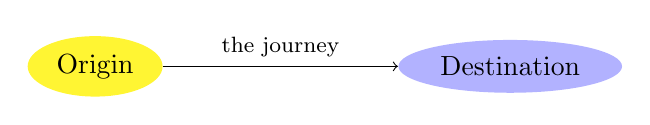
\begin{tikzpicture}
        \node[fill=yellow!80,ellipse] (origin) {Origin};
        \node[fill=blue!30,ellipse] (destination) at (15em,0) {Destination};
        \path (origin) edge[->] node[above,font=\footnotesize] {the journey}
        (destination);
    \end{tikzpicture}
    \caption{TikZ drawings will be output as SVG, which should be rendered by most modern browsers.}
\end{figure}

\begin{figure}[!ht]
    \centering
    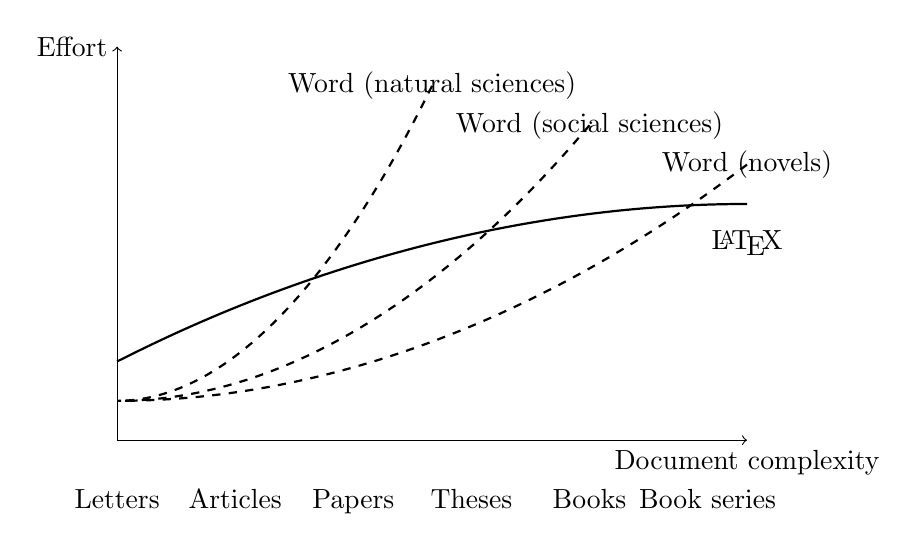
\begin{tikzpicture}

    % horizontal axis
    \draw[->] (0,0) -- (8,0) node[anchor=north] {Document complexity};
    \draw[->] (0,0) -- (0,5) node[anchor=east] {Effort};
    
    % labels
    \draw	(0,-0.5) node[anchor=north] {Letters}
    		(1.5,-0.5) node[anchor=north] {Articles}
    		(3,-0.5) node[anchor=north] {Papers}
    		(4.5,-0.5) node[anchor=north] {Theses}
    		(6,-0.5) node[anchor=north] {Books}
    		(7.5,-0.5) node[anchor=north] {Book series};
    
    \draw (8,3.5) node {Word (novels)};
    \draw (6,4) node {Word (social sciences)};
    \draw (4,4.5) node {Word (natural sciences)};
    \draw (8,2.5) node {\LaTeX{}};
    
    % Psis
    \draw[thick,dashed] (8,3.5) parabola[bend at end] (0,0.5);
    \draw[thick,dashed] (6,4) parabola[bend at end] (0,0.5);
    \draw[thick,dashed] (4,4.5) parabola[bend at end] (0,0.5);
    \draw[thick] (0,1) parabola[bend at end] (8,3);

\end{tikzpicture}
    \caption{Comparing complexity of \textit{Word} and \LaTeX{} depending on the application.}\label{fig:latexeffortcomplexity}
\end{figure}

\begin{figure}[!ht]
    \centering
    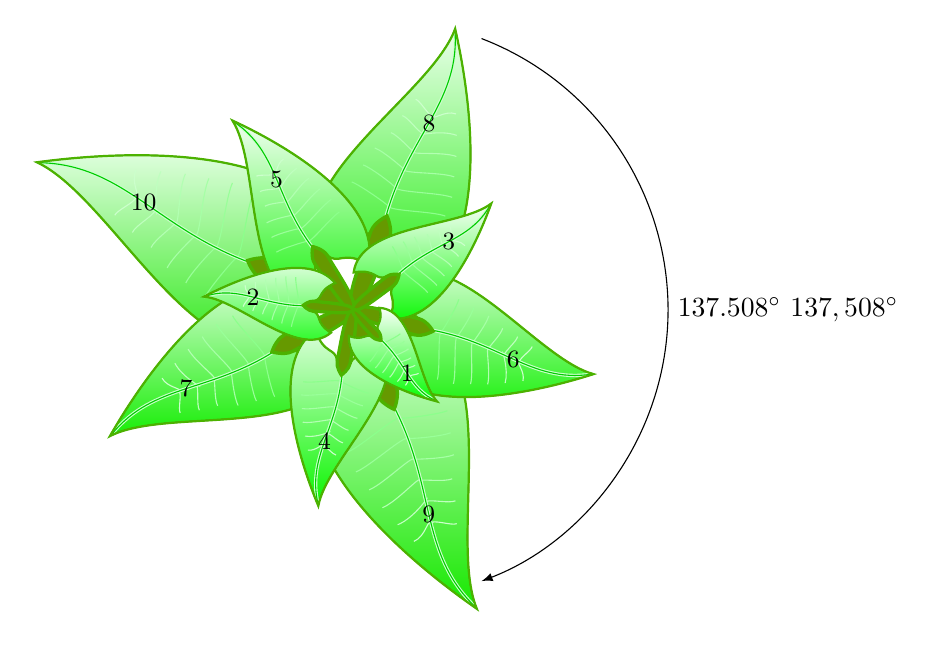
\begin{tikzpicture}
    \foreach \x in {10,...,1}
    {\draw[shade,bottom color=red!\x!green,top color=green!\x,x=0.3 pt,y=0.3 pt,scale={0.4+0.1*\x},rotate=222.5*\x] (0,0) .. 
    controls ( -11,  1) and ( -9, 50) .. (-10,80) ..
    controls ( -16, 60) and (-32, 75) .. (-50,40) .. 
    controls (-110,100) and (-0,230) ..  (  0,300)  node[below] (\x) {} ..
    controls (  45,230) and (110,100) .. ( 50,40) ..
    controls (  32, 75) and ( 16, 60) ..  ( 10,80) ..
    controls (   9, 50) and ( 11,  1) .. (  0,0) 
    -- cycle ;
    
    \draw[thin,green!45,x=0.3 pt,y=0.3 pt,scale={0.4+0.1*\x},rotate=222.5*\x] (-45,120) .. controls (-35,120) and (0,110) .. (-3,110) .. controls (0,105) and (40,120) .. (55,120);
    \draw[thin,green!40,x=0.3 pt,y=0.3 pt,scale={0.4+0.1*\x},rotate=222.5*\x] (-40,140) .. controls (-30,140) and (0,130) .. (-3,130) .. controls (0,125) and (40,140) .. (55,140);
    \draw[thin,green!35,x=0.3 pt,y=0.3 pt,scale={0.4+0.1*\x},rotate=222.5*\x] (-35,160) .. controls (-25,160) and (0,150) .. (0,150) .. controls (0,145) and (35,160) .. (50,160);
    \draw[thin,green!30,x=0.3 pt,y=0.3 pt,scale={0.4+0.1*\x},rotate=222.5*\x] (-25,180) .. controls (-17,180) and (0,170) .. (3,170) .. controls (0,165) and (30,180) .. (45,180);
    \draw[thin,green!25,x=0.3 pt,y=0.3 pt,scale={0.4+0.1*\x},rotate=222.5*\x] (-20,200) .. controls (-13,200) and (0,190) .. (6,190) .. controls (0,185) and (20,200) .. (38,200);
    \draw[thin,green!20,x=0.3 pt,y=0.3 pt,scale={0.4+0.1*\x},rotate=222.5*\x] (-13,220) .. controls (-8,220) and (3,210) .. (8,210) .. controls (10,205) and (18,220) .. (30,220);
    \draw[very thick,green!20,x=0.3 pt,y=0.3 pt,scale={0.4+0.1*\x},rotate=222.5*\x] (0,90) .. controls (-10,180) and (30,230) .. (1,297);
    \draw[thin,black!20!green,x=0.3 pt,y=0.3 pt,scale={0.4+0.1*\x},rotate=222.5*\x] (0,90)  .. controls (-10,180) and (30,230)  .. (1,297) node[midway,black] (num\x) {\small\x};
    \draw[very thick,red!30!green,fill=red!40!green,x=0.3 pt,y=0.3 pt,scale={0.4+0.1*\x},rotate=222.5*\x] 
    (0,0) .. 
    controls ( -11,  1) and ( -9, 50) ..
    (-10,80) .. 
    controls (-10,90) and (0,100) .. (0,100) ..
    controls (0,100) and (10,90) .. (10,80)..
    controls (   9, 50) and ( 11,  1) .. (  0,0) 
    -- cycle;
    \draw[thick,red!30!green,x=0.3 pt,y=0.3 pt,scale={0.4+0.1*\x},rotate=222.5*\x] (0,0) .. 
    controls ( -11,  1) and ( -9, 50) .. (-10,80) ..
    controls ( -16, 60) and (-32, 75) .. (-50,40) .. 
    controls (-110,100) and (-0,230) ..  (  0,300) ..
    controls (  45,230) and (110,100) .. ( 50,40) ..
    controls (  32, 75) and ( 16, 60) ..  ( 10,80) ..
    controls (   9, 50) and ( 11,  1) .. (  0,0) 
    -- cycle ;
    }
    \draw[->,>=latex,x=0.3 pt,y=0.3 pt,black] ([xshift=6pt] 8.east) arc (69:-69:350) node[midway,right] {$137.508^\circ$ $137,508^\circ$};
\end{tikzpicture}

    \caption{Example of a drawing made in TikZ.}\label{fig:leaves-golden-cut}
\end{figure}

\begin{figure}[!ht]
    \centering
    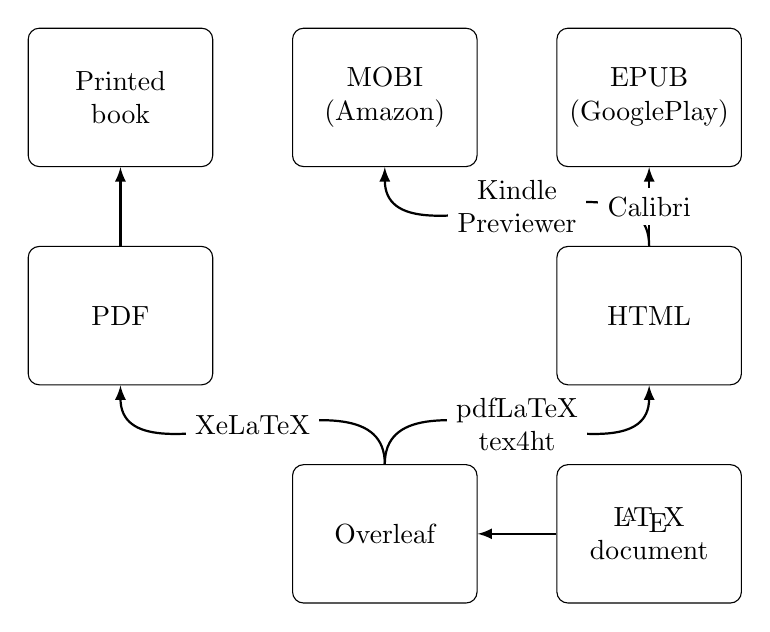
\begin{tikzpicture}
    % Define styles of various tikz elements.
    \tikzstyle{textbox} = [rounded corners, text width=60pt, minimum height=50pt,text centered,draw=black]
    \tikzstyle{arrow} = [thick,->,>=latex]
    \tikzstyle{block} = [rectangle,textbox]
    \tikzstyle{textarr} = [rectangle,align=center,fill=white]

    \node (latex) [block] {\LaTeX{}\\document};
    \node (overleaf) [block, left=of latex] {Overleaf};
    \node (pdf) [block, above left=of overleaf] {PDF}; % xelatex
    \node (html) [block, above right=of overleaf] {HTML}; % pdfLaTeX + tex4ht
    
    \node (print) [block, above= of pdf] {Printed\\book};
    \node (mobi) [block, above left=of html] {MOBI\\(Amazon)}; % Kindle Previewer
    \node (epub) [block, above= of html] {EPUB\\(GooglePlay)}; % Calibri
    
    \draw[out=90,in=270] [arrow] (overleaf) to node[textarr] {XeLaTeX} (pdf);
    \draw[out=90,in=270] [arrow] (overleaf) to node[textarr] {pdfLaTeX\\tex4ht} (html);
    
    \draw [arrow] (latex) -- (overleaf);
    \draw [arrow] (pdf) -- (print);
    
    \draw[out=90,in=270] [arrow] (html) to node[textarr] {Kindle\\Previewer} (mobi);
    \draw [arrow] (html) -- node[textarr] {Calibri} (epub);
\end{tikzpicture}
    \caption{Example 2 of a drawing made in TikZ.}\label{fig:buildchain}
\end{figure}
%test
\end{document}